% Options for packages loaded elsewhere
\PassOptionsToPackage{unicode}{hyperref}
\PassOptionsToPackage{hyphens}{url}
\PassOptionsToPackage{dvipsnames,svgnames,x11names}{xcolor}
%
\documentclass[
  10pt,
  letterpaper,
]{book}

\usepackage{amsmath,amssymb}
\usepackage{iftex}
\ifPDFTeX
  \usepackage[T1]{fontenc}
  \usepackage[utf8]{inputenc}
  \usepackage{textcomp} % provide euro and other symbols
\else % if luatex or xetex
  \usepackage{unicode-math}
  \defaultfontfeatures{Scale=MatchLowercase}
  \defaultfontfeatures[\rmfamily]{Ligatures=TeX,Scale=1}
\fi
\usepackage{lmodern}
\ifPDFTeX\else  
    % xetex/luatex font selection
\fi
% Use upquote if available, for straight quotes in verbatim environments
\IfFileExists{upquote.sty}{\usepackage{upquote}}{}
\IfFileExists{microtype.sty}{% use microtype if available
  \usepackage[]{microtype}
  \UseMicrotypeSet[protrusion]{basicmath} % disable protrusion for tt fonts
}{}
\makeatletter
\@ifundefined{KOMAClassName}{% if non-KOMA class
  \IfFileExists{parskip.sty}{%
    \usepackage{parskip}
  }{% else
    \setlength{\parindent}{0pt}
    \setlength{\parskip}{6pt plus 2pt minus 1pt}}
}{% if KOMA class
  \KOMAoptions{parskip=half}}
\makeatother
\usepackage{xcolor}
\usepackage[a5paper,top=2.5cm,bottom=1cm,left=1cm,right=1cm]{geometry}
\setlength{\emergencystretch}{3em} % prevent overfull lines
\setcounter{secnumdepth}{5}
% Make \paragraph and \subparagraph free-standing
\ifx\paragraph\undefined\else
  \let\oldparagraph\paragraph
  \renewcommand{\paragraph}[1]{\oldparagraph{#1}\mbox{}}
\fi
\ifx\subparagraph\undefined\else
  \let\oldsubparagraph\subparagraph
  \renewcommand{\subparagraph}[1]{\oldsubparagraph{#1}\mbox{}}
\fi


\providecommand{\tightlist}{%
  \setlength{\itemsep}{0pt}\setlength{\parskip}{0pt}}\usepackage{longtable,booktabs,array}
\usepackage{calc} % for calculating minipage widths
% Correct order of tables after \paragraph or \subparagraph
\usepackage{etoolbox}
\makeatletter
\patchcmd\longtable{\par}{\if@noskipsec\mbox{}\fi\par}{}{}
\makeatother
% Allow footnotes in longtable head/foot
\IfFileExists{footnotehyper.sty}{\usepackage{footnotehyper}}{\usepackage{footnote}}
\makesavenoteenv{longtable}
\usepackage{graphicx}
\makeatletter
\def\maxwidth{\ifdim\Gin@nat@width>\linewidth\linewidth\else\Gin@nat@width\fi}
\def\maxheight{\ifdim\Gin@nat@height>\textheight\textheight\else\Gin@nat@height\fi}
\makeatother
% Scale images if necessary, so that they will not overflow the page
% margins by default, and it is still possible to overwrite the defaults
% using explicit options in \includegraphics[width, height, ...]{}
\setkeys{Gin}{width=\maxwidth,height=\maxheight,keepaspectratio}
% Set default figure placement to htbp
\makeatletter
\def\fps@figure{htbp}
\makeatother
% definitions for citeproc citations
\NewDocumentCommand\citeproctext{}{}
\NewDocumentCommand\citeproc{mm}{%
  \begingroup\def\citeproctext{#2}\cite{#1}\endgroup}
\makeatletter
 % allow citations to break across lines
 \let\@cite@ofmt\@firstofone
 % avoid brackets around text for \cite:
 \def\@biblabel#1{}
 \def\@cite#1#2{{#1\if@tempswa , #2\fi}}
\makeatother
\newlength{\cslhangindent}
\setlength{\cslhangindent}{1.5em}
\newlength{\csllabelwidth}
\setlength{\csllabelwidth}{3em}
\newenvironment{CSLReferences}[2] % #1 hanging-indent, #2 entry-spacing
 {\begin{list}{}{%
  \setlength{\itemindent}{0pt}
  \setlength{\leftmargin}{0pt}
  \setlength{\parsep}{0pt}
  % turn on hanging indent if param 1 is 1
  \ifodd #1
   \setlength{\leftmargin}{\cslhangindent}
   \setlength{\itemindent}{-1\cslhangindent}
  \fi
  % set entry spacing
  \setlength{\itemsep}{#2\baselineskip}}}
 {\end{list}}
\usepackage{calc}
\newcommand{\CSLBlock}[1]{\hfill\break\parbox[t]{\linewidth}{\strut\ignorespaces#1\strut}}
\newcommand{\CSLLeftMargin}[1]{\parbox[t]{\csllabelwidth}{\strut#1\strut}}
\newcommand{\CSLRightInline}[1]{\parbox[t]{\linewidth - \csllabelwidth}{\strut#1\strut}}
\newcommand{\CSLIndent}[1]{\hspace{\cslhangindent}#1}

% Cargar fuentes y paquetes de estilo
\usepackage{fontspec}
\usepackage{emoji}
\setmainfont{EB Garamond}        
\usepackage{xcolor}
\definecolor{highlight}{RGB}{29, 120, 200} 

% Paquetes para tablas responsivas
\usepackage{graphicx}     % Para \resizebox
\usepackage{tabularx}     % Para tablas de ancho adaptable
\usepackage[raggedrightboxes]{ragged2e} 

% Paquete para soporte de idiomas
\usepackage{polyglossia}
\setmainlanguage{spanish} 

% Microtipografía avanzada
\usepackage[activate={true,nocompatibility},final,tracking=true,kerning=true,spacing=true,factor=1100,stretch=10,shrink=10]{microtype}

\widowpenalty=10000
\clubpenalty=10000

% Control de ríos (ligeramente ragged right)
\usepackage[raggedrightboxes]{ragged2e}

% Gestión de guiones
\hyphenpenalty=50 
\exhyphenpenalty=50 
\emergencystretch=3em

% Paquete para la personalización del título
\usepackage{titling}

% Configuración de encabezados y pies de página
\usepackage{fancyhdr}
\pagestyle{fancy}
\fancyhf{}
\fancyhead[LE,RO]{\thepage} 
\fancyhead[RE]{\nouppercase{\leftmark}} 
\fancyhead[LO]{\nouppercase{\rightmark}}   

\fancyfoot[C]{\thepage}
\makeatletter
\@ifpackageloaded{bookmark}{}{\usepackage{bookmark}}
\makeatother
\makeatletter
\@ifpackageloaded{caption}{}{\usepackage{caption}}
\AtBeginDocument{%
\ifdefined\contentsname
  \renewcommand*\contentsname{Table of contents}
\else
  \newcommand\contentsname{Table of contents}
\fi
\ifdefined\listfigurename
  \renewcommand*\listfigurename{List of Figures}
\else
  \newcommand\listfigurename{List of Figures}
\fi
\ifdefined\listtablename
  \renewcommand*\listtablename{List of Tables}
\else
  \newcommand\listtablename{List of Tables}
\fi
\ifdefined\figurename
  \renewcommand*\figurename{Figure}
\else
  \newcommand\figurename{Figure}
\fi
\ifdefined\tablename
  \renewcommand*\tablename{Table}
\else
  \newcommand\tablename{Table}
\fi
}
\@ifpackageloaded{float}{}{\usepackage{float}}
\floatstyle{ruled}
\@ifundefined{c@chapter}{\newfloat{codelisting}{h}{lop}}{\newfloat{codelisting}{h}{lop}[chapter]}
\floatname{codelisting}{Listing}
\newcommand*\listoflistings{\listof{codelisting}{List of Listings}}
\makeatother
\makeatletter
\makeatother
\makeatletter
\@ifpackageloaded{caption}{}{\usepackage{caption}}
\@ifpackageloaded{subcaption}{}{\usepackage{subcaption}}
\makeatother
\ifLuaTeX
  \usepackage{selnolig}  % disable illegal ligatures
\fi
\usepackage{bookmark}

\IfFileExists{xurl.sty}{\usepackage{xurl}}{} % add URL line breaks if available
\urlstyle{same} % disable monospaced font for URLs
\hypersetup{
  pdftitle={iabookMaquiloca},
  pdfauthor={Javier Flores},
  colorlinks=true,
  linkcolor={highlight},
  filecolor={Maroon},
  citecolor={Blue},
  urlcolor={highlight},
  pdfcreator={LaTeX via pandoc}}

\title{iabookMaquiloca}
\author{Javier Flores}
\date{2024-09-25}

\begin{document}
\frontmatter
\maketitle

\renewcommand*\contentsname{Table of contents}
{
\hypersetup{linkcolor=}
\setcounter{tocdepth}{2}
\tableofcontents
}
\mainmatter
\bookmarksetup{startatroot}

\chapter*{Impacto de la Inteligencia
Artificial}\label{impacto-de-la-inteligencia-artificial}
\addcontentsline{toc}{chapter}{Impacto de la Inteligencia Artificial}

\markboth{Impacto de la Inteligencia Artificial}{Impacto de la
Inteligencia Artificial}

\textbackslash begin\{document\}

\section*{Introducción}\label{introducciuxf3n}
\addcontentsline{toc}{section}{Introducción}

\markright{Introducción}

Ciudad Juárez, crisol de culturas y encrucijada de industrias, se
encuentra en el umbral de una nueva era. La inteligencia artificial, esa
fuerza transformadora que redefine los límites de lo posible, está
llegando a las entrañas de la maquiladora, prometiendo una revolución
silenciosa pero profunda.

Este libro es un viaje a través de esa revolución. Exploraremos cómo la
IA está cambiando la forma en que se produce, se innova y se compite en
la frontera. Desde los robots que comparten espacio con los trabajadores
en la línea de montaje, hasta los algoritmos que predicen la demanda del
mercado con una precisión asombrosa, la IA está dejando su huella en
cada rincón de la industria.

Pero este libro no es solo sobre tecnología. Es sobre las personas que
dan vida a la maquiladora, los hombres y mujeres cuya labor diaria
construye el futuro de Juárez. Es sobre cómo la IA puede empoderarlos,
liberándolos de tareas repetitivas y peligrosas, y permitiéndoles
desarrollar todo su potencial creativo.

Y es, sobre todo, un homenaje a Ciudad Juárez, mi ciudad, esa tierra
indomable que siempre ha sabido reinventarse frente a la adversidad. Que
este libro sea un testimonio de su espíritu innovador, de su capacidad
para abrazar el cambio y forjar un futuro más próspero para todos.

\section*{Objetivo General}\label{objetivo-general}
\addcontentsline{toc}{section}{Objetivo General}

\markright{Objetivo General}

El objetivo de este libro es mostrar cómo la inteligencia artificial
(IA) está transformando la industria maquiladora en Ciudad Juárez,
explicando de forma clara y accesible cómo esta tecnología puede mejorar
la productividad, la eficiencia y las condiciones laborales. Está
dirigido tanto a los líderes que buscan implementar IA en sus fábricas,
a los estudiantes que quieren entender las nuevas tendencias
tecnológicas, y a los trabajadores de la maquila, para que vean cómo la
IA puede hacer sus vidas más fáciles sin temor a perder su trabajo.

A través de ejemplos prácticos, casos reales y una explicación sencilla,
este libro pretende ser una guía para que Ciudad Juárez siga siendo
competitiva en el mercado global, mientras empodera a las personas que
día a día hacen posible el funcionamiento de las maquilas.

\section*{Dedicatoria}\label{dedicatoria}
\addcontentsline{toc}{section}{Dedicatoria}

\markright{Dedicatoria}

A Ciudad Juárez, mi hogar, mi inspiración. A su gente trabajadora y
resiliente, que día a día construye un futuro mejor. Y a la memoria de
mi novia Alejandra Mendez, quien siempre creyó en mí y en el potencial
de esta ciudad.

\section*{Agradecimientos}\label{agradecimientos}
\addcontentsline{toc}{section}{Agradecimientos}

\markright{Agradecimientos}

Al equipo del IACenter, especialmente a Eduardo Castillo y Joam Ricon,
por su apoyo incondicional y su visión compartida. A todos los expertos
y profesionales que contribuyeron con sus conocimientos y experiencias a
este libro. Y a mi familia y amigos, por su amor y aliento constantes.

\section*{Público Objetivo}\label{puxfablico-objetivo}
\addcontentsline{toc}{section}{Público Objetivo}

\markright{Público Objetivo}

Este libro está pensado para tres grandes grupos: los \textbf{líderes de
la industria maquiladora}, los \textbf{estudiantes} que se están
adentrando en el mundo de la manufactura, y los \textbf{trabajadores de
la maquila} que viven día a día en las líneas de producción. Aunque cada
grupo tiene un enfoque distinto, todos comparten un interés en entender
cómo la inteligencia artificial está cambiando la maquila y cómo esto
impacta sus vidas y carreras.

\subsubsection*{1. Para los líderes de la
maquila:}\label{para-los-luxedderes-de-la-maquila}
\addcontentsline{toc}{subsubsection}{1. Para los líderes de la maquila:}

Si estás a cargo de una maquiladora o tienes un puesto de liderazgo,
aquí vas a encontrar las estrategias que necesitas para \textbf{mantener
tu maquila al frente de la competencia}. Este libro te va a guiar para
entender no solo \textbf{cómo aplicar la IA} en tus procesos, sino
también cómo \textbf{preparar a tu equipo} para los cambios que vienen.
La clave está en saber \textbf{qué decisiones tomar} para que tu maquila
siga siendo eficiente, rentable y competitiva en el mercado global.

Te vas a topar con temas como la automatización, el Machine Learning, y
\textbf{cómo usar la IA para reducir costos y mejorar la producción},
pero siempre aterrizados a la realidad de las maquiladoras de Ciudad
Juárez. No se trata de meter pura tecnología por meter, sino de
\textbf{hacer más con menos} y \textbf{sacar el mejor provecho de lo que
ya tienes}. Este libro es tu guía para no quedarte atrás en esta nueva
revolución tecnológica.

\subsubsection*{2. Para los estudiantes:}\label{para-los-estudiantes}
\addcontentsline{toc}{subsubsection}{2. Para los estudiantes:}

Si apenas te estás metiendo al mundo de la manufactura o te interesa
entender más sobre la \textbf{inteligencia artificial}, este libro te
explica lo básico de manera sencilla, sin tanta vuelta técnica. Aquí
aprenderás \textbf{cómo la IA está siendo usada} en las maquilas de
Juárez y \textbf{cómo va a cambiar las cosas} en el futuro cercano.
Desde los \textbf{fundamentos de la IA} hasta ejemplos prácticos en las
fábricas, vas a ver \textbf{cómo se conectan la teoría y la práctica}.

Este libro está pensado para que, aunque no seas un experto en
tecnología, \textbf{entiendas lo suficiente} como para empezar a pensar
en \textbf{cómo la IA puede mejorar los procesos} y hasta cómo te puede
ayudar en tu carrera. La tecnología avanza rápido, y este libro es tu
chance de \textbf{ponerte al tiro} y estar listo para aprovechar las
oportunidades que vienen.

\subsubsection*{3. Para los trabajadores de la
maquila:}\label{para-los-trabajadores-de-la-maquila}
\addcontentsline{toc}{subsubsection}{3. Para los trabajadores de la
maquila:}

Este libro también es para ti, \textbf{compa de la línea}. Si eres de
los que todos los días le entra duro al trabajo en la maquila, este
libro te va a ayudar a entender \textbf{qué onda con la IA} y cómo va a
cambiar las cosas en tu jale. No te asustes, que no todo se trata de
robots quitando empleos. Al contrario, lo que la IA puede hacer es
\textbf{quitarte esas tareas repetitivas y pesadas}, para que te
enfoques en cosas más interesantes y creativas.

Te voy a explicar \textbf{sin tanto rollo técnico} cómo están usando ya
la inteligencia artificial en las fábricas para mejorar la producción y
\textbf{hacer las cosas más fáciles} para todos. Desde los
\textbf{robots que trabajan a tu lado}, hasta las máquinas que aprenden
de los errores y \textbf{evitan problemas antes de que pasen}, la IA es
una herramienta que \textbf{puede ayudarte a hacer mejor tu trabajo y de
manera más segura}.

La idea es que no sientas que la tecnología viene a complicarte la vida,
sino que entiendas \textbf{cómo puedes aprovecharla para que la jala sea
menos pesada y más eficiente}. Así que si te late saber \textbf{cómo
está cambiando la maquila} y qué puedes esperar en los próximos años,
este libro es para ti.

\subsection*{Por Qué Escribo Así: Términos Juarenses en Este
Libro}\label{por-quuxe9-escribo-asuxed-tuxe9rminos-juarenses-en-este-libro}
\addcontentsline{toc}{subsection}{Por Qué Escribo Así: Términos
Juarenses en Este Libro}

Este libro está escrito de una manera que mezcla lo técnico con lo
cotidiano, y no es casualidad que se usen términos y expresiones propias
de Ciudad Juárez. ¿Por qué? Pues porque cuando hablamos de la maquila y
su impacto en nuestra región, no podemos desligar la historia de la
gente que la ha hecho posible: los juarenses. La maquila no es solo
máquinas y producción, es también el esfuerzo, la lucha y la identidad
de la gente que día a día se rifa en este ambiente.

Al usar jerga juarense, quiero que el libro se sienta cercano, como si
estuvieras platicando con un compa que sabe del tema. Es una forma de
hacer que los conceptos no se sientan tan lejanos o técnicos, sino más
bien como algo que está al alcance de todos, algo que puedes entender y
aplicar sin sentir que estás leyendo un manual aburrido.

Además, el uso de esta jerga es un homenaje a nuestra cultura
fronteriza. La forma en que hablamos aquí es única, refleja nuestra
historia y nuestra realidad. Al usar estas expresiones, estoy diciendo
que este libro no es solo para expertos de laboratorio o para aquellos
que manejan conceptos complicados, sino para la gente de Juárez, que
vive y respira la maquila, y que entiende las cosas mejor cuando se les
habla en su propio idioma.

Así que, si en algún momento te encuentras con términos o expresiones
que te suenan muy de aquí, no te saques de onda. Es parte de lo que
somos, y de lo que quiero compartir contigo en este libro.

\bookmarksetup{startatroot}

\chapter{La Industria Maquiladora en Ciudad
Juárez}\label{la-industria-maquiladora-en-ciudad-juuxe1rez}

\section{Evolución Histórica de la Industria Maquiladora en Ciudad
Juárez}\label{evoluciuxf3n-histuxf3rica-de-la-industria-maquiladora-en-ciudad-juuxe1rez}

\subsection{Contexto Histórico: El Surgimiento de la Industria en Ciudad
Juárez}\label{contexto-histuxf3rico-el-surgimiento-de-la-industria-en-ciudad-juuxe1rez}

Ciudad Juárez, antes de que la maquila se convirtiera en la estrella del
show, era un lugar donde la gente se rifaba la vida con lo que podía. En
los cuarentas, la ciudad empezó a crecer a lo loco gracias al turismo,
el comercio en la frontera y la migración. Era la época donde se
levantaron fábricas pequeñas, que producían de todo, desde jabón hasta
whiskey. Sin embargo, este crecimiento industrial inicial se vio frenado
por la llegada de la Segunda Guerra Mundial, un evento que cambiaría
radicalmente el panorama económico de la región. Los estadounidenses
comenzaron a pedir mano de obra de forma masiva, y muchos trabajadores
locales cruzaron la frontera para encontrar empleo, lo que dejó muchas
fábricas en Ciudad Juárez con falta de personal {[}1{]}.

Mientras tanto, Fort Bliss se llenó de soldados que, cuando no estaban
en el cuartel, se venían para Juárez a tirar relajo. Eso levantó un
chorro el turismo y los servicios, y de paso, empezó a cambiar la
economía de la ciudad {[}1{]}. Fue en ese tiempo que Juárez empezó a
transformarse en lo que es ahora, una ciudad que, aunque siempre ha sido
fronteriza, empezaba a ver cómo el dinero entraba por otras vías, no
solo por la agricultura.

\subsection{El Programa Bracero y su Impacto en el Desarrollo Industrial
de Ciudad
Juárez}\label{el-programa-bracero-y-su-impacto-en-el-desarrollo-industrial-de-ciudad-juuxe1rez}

Para cuando llegó el 42, Estados Unidos lanzó el Programa Bracero porque
necesitaba manos que le echaran al jale en los campos. Y pues Juárez,
por estar cerquita, se convirtió en un punto clave. La raza se iba en
bola para trabajar allá, y eso trajo mucha lana a la ciudad {[}1{]}.
Pero la cosa se puso fea cuando en los sesentas la agricultura empezó a
dar bajón, y los braceros que regresaban se encontraban con que ya no
había mucho que hacer acá. La ciudad se llenó de desempleados, y el
panorama no pintaba nada bien {[}1{]}.

Ya para el 65, cuando se acabó el Programa Bracero, la cosa estaba color
de hormiga. La industria que quedaba no daba para tanto, y la ciudad
estaba llena de gente que no sabía para dónde jalar. Fue entonces cuando
el gobierno federal le entró al quite con el PRONAF y el Programa de
Industrialización Fronteriza (PIF) {[}1{]}. La idea era darle un
levantón a la economía de la frontera, y Juárez, con su ubicación chida,
fue uno de los lugares donde estos programas pegaron más fuerte.

\subsection{Nacimiento y Consolidación de la Industria Maquiladora: De
los 60s a los
80s}\label{nacimiento-y-consolidaciuxf3n-de-la-industria-maquiladora-de-los-60s-a-los-80s}

El verdadero trancazo vino con el PIF en 1965. Ahí fue cuando Juárez
empezó a ser lo que es hoy. Gracias a ese programa, un montón de
empresas estadounidenses comenzaron a instalar sus plantas de ensamblaje
en la ciudad, aprovechando la mano de obra barata y la cercanía con el
mercado estadounidense. Este impulso inicial no solo permitió a la
región recuperar el empleo perdido, sino que también estableció las
bases para el crecimiento sostenido de la maquiladora en los años
posteriores. Para finales de los sesentas, México ya se codeaba con los
grandes en la industria maquiladora, solo detrás de Alemania y Canadá.
Este éxito fue apenas el comienzo, ya que en las décadas siguientes la
maquiladora se consolidaría como el motor económico de la ciudad. A
continuación, exploraremos cómo las políticas gubernamentales y las
inversiones extranjeras fortalecieron aún más esta industria a lo largo
de los 70s y 80s {[}3{]}.

Juárez se convirtió en un imán para estas empresas. Para finales de los
sesentas, México ya se codeaba con los grandes en la industria
maquiladora, solo detrás de Alemania y Canadá {[}4{]}. Empresas como
RCA, Coilcraft, y Acapulco Fashion pusieron sus ojos en la ciudad, y así
Juárez se convirtió en un mero centro de maquilas {[}5{]}. El billete
empezó a correr y con él, la ciudad comenzó a cambiar de cara.

\begin{figure}[H]

{\centering 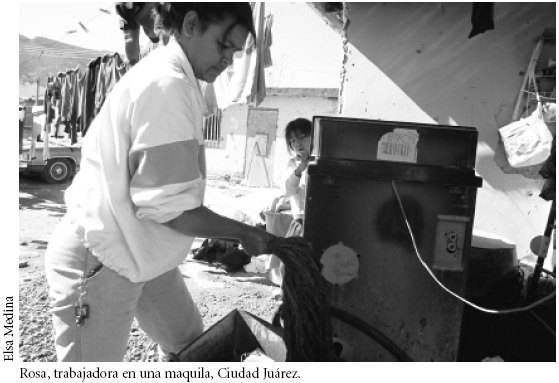
\includegraphics{Img/Rosa.jpg}

}

\caption{Rosa}

\end{figure}%

\subsection{Crecimiento Descontrolado y Desafíos Urbanos en los 70s y
80s}\label{crecimiento-descontrolado-y-desafuxedos-urbanos-en-los-70s-y-80s}

Ya en los setentas, la maquila era la que rifaba en Juárez. Empleaba a
un chorro de gente, sobre todo a las morras, que eran las que más jale
encontraban en las fábricas de textiles y electrónica {[}6{]}. Pero como
todo en la vida, no todo era miel sobre hojuelas. El crecimiento fue tan
rápido que la ciudad no estaba preparada para tanta gente. Juárez creció
como mancha de aceite, con colonias que brotaban por todos lados, muchas
sin agua, drenaje ni pavimento {[}7{]}.

Las maquilas se instalaban donde les daba la gana, y eso hizo que el
crecimiento urbano fuera un desmadre {[}1{]}. La falta de planificación
hizo que muchas colonias se quedaran sin servicios básicos, y la ciudad,
en lugar de crecer con orden, lo hizo a lo loco. Aun así, la maquila
seguía siendo la que mandaba, y la raza, a pesar de las broncas, no
dejaba de jalar porque, como dicen por aquí, la jale es la jale.

\subsection{Crisis y Resiliencia en la
Maquiladora}\label{crisis-y-resiliencia-en-la-maquiladora}

Pero no todo fue éxito. En 1974, Juárez se enfrentó a su primera gran
crisis en la maquila cuando la empresa Transformer de México cerró,
dejando a 300 trabajadores en la calle {[}8{]}. La recesión en Estados
Unidos pegó duro, y varias maquilas que dependían del mercado gringo se
vieron en la necesidad de bajar cortinas {[}8{]}. La crisis se volvió a
sentir en 1980, cuando varias fábricas tuvieron que reducir operaciones
o cerrar temporalmente por falta de materia prima y sobreproducción
{[}9{]}.

A pesar de estos golpes, la maquila en Juárez demostró que estaba hecha
de otra madera. En 1983, ya andaba operando al 85\% de su capacidad, y
para 1984, se esperaba que la cosa mejorara aún más con la llegada de
nuevas empresas {[}10{]}{[}11{]}. Fue durante los ochentas cuando Juárez
empezó a atraer a empresas de alta tecnología, marcando una nueva etapa
en la historia de la maquila en la ciudad {[}11{]}. La resiliencia de
Juárez frente a las crisis mostró que, aunque las cosas se pusieran
difíciles, la ciudad siempre encontraba la manera de salir adelante.

\subsection{Evolución Reciente y Desafíos
Modernos}\label{evoluciuxf3n-reciente-y-desafuxedos-modernos}

En los últimos años, la industria maquiladora en Ciudad Juárez ha
seguido siendo un motor económico crucial. Sin embargo, ha tenido que
adaptarse a nuevos desafíos, como la digitalización, la automatización y
los cambios en las cadenas de suministro globales. El impacto de la
pandemia de COVID-19 también obligó a las maquilas a reinventar sus
procesos para mantener la producción en marcha, implementando nuevas
tecnologías y protocolos de seguridad {[}12{]}.

El informe de la Secretaría de Economía de 2022 destaca cómo la
industria maquiladora ha empezado a integrar tecnologías como la
inteligencia artificial y el Internet de las Cosas (IoT) para optimizar
la producción y reducir costos {[}13{]}. Esto ha llevado a una
transformación en la forma en que operan las maquilas, con un enfoque
cada vez mayor en la innovación y la sostenibilidad.

\begin{figure}[H]

{\centering 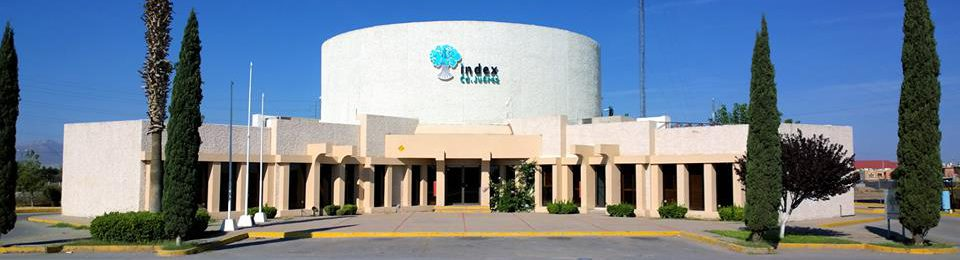
\includegraphics{Img/Amac.jpg}

}

\caption{Amac}

\end{figure}%

\subsection{Referencias}\label{referencias}

\begin{enumerate}
\def\labelenumi{\arabic{enumi}.}
\tightlist
\item
  Oscar Martínez, \emph{Ciudad Juárez: El auge de una ciudad fronteriza
  a partir de 1848}, FCE, México, 1982.
\item
  ``La Frontera norte, diagnóstico y perspectivas'', Dirección General
  de Estadística, S.I.C. s/f, mimeo.
\item
  Thomas Madison, \emph{Reseña anual de la industria maquiladora},
  SUGUMEX, México, 1990.
\item
  Bass Zavala, Sonia. ``El crecimiento urbano en Ciudad Juárez,
  1950-2000. Un acercamiento socio-histórico a la evolución desordenada
  de una ciudad de la frontera norte.'' \emph{Chihuahua Hoy} (2013):
  247-289.
\item
  ``La Frontera norte, diagnóstico y perspectivas'', Dirección General
  de Estadística, S.I.C. s/f, mimeo.
\item
  Diario de Juárez, 21 a 24 de agosto de 1981.
\item
  El Fronterizo, 25 de agosto de 1974.
\item
  Guadalupe Ramos, Norte, 9 de febrero de 1994, p.~4A.
\item
  Diario de Juárez, 22 de mayo de 1991.
\item
  Diario de Juárez, 7 de febrero de 1991.
\item
  Declaración de José Manuel Luna, promotor de AMACH, \emph{Novedades},
  20 de enero de 1985.
\item
  Vega, Luis. ``La transformación de la industria maquiladora en la era
  digital.'' \emph{El Financiero}, 2023.
\item
  Secretaría de Economía. ``Informe Anual sobre la Industria
  Maquiladora''. Gobierno de México, 2022.
\end{enumerate}

\bookmarksetup{startatroot}

\chapter{Fundamentos clave de la IA en la
Maquiladora}\label{fundamentos-clave-de-la-ia-en-la-maquiladora}

\section{Concepto de IA en la
Industria}\label{concepto-de-ia-en-la-industria}

La Inteligencia Artificial (IA) es un término que ha sido parte de la
conversación tecnológica desde hace décadas. Aunque a veces parece un
concepto moderno, sus raíces vienen de los años 50, cuando pioneros como
\textbf{John McCarthy} y \textbf{Herbert A. Simon} empezaron a hablar
sobre la idea de hacer que las máquinas ``piensen'' de manera similar a
los humanos. Según McCarthy, la IA se trata de ``la ciencia e ingeniería
de hacer que las máquinas se comporten de manera inteligente.'' Pero,
¿qué significa esto en términos más simples?

En su libro clásico \textbf{``Las Ciencias de lo Artificial''} (1969),
Simon describió la IA como la habilidad de una máquina para imitar el
pensamiento humano en la toma de decisiones y la resolución de
problemas. Estas ideas nos ayudan a entender que la IA no es magia, sino
una tecnología diseñada para analizar datos, aprender de ellos, y actuar
en consecuencia, a menudo siguiendo reglas o patrones.

Estas ideas fundacionales, aunque teóricas en su origen, sentaron las
bases de lo que hoy vemos en las fábricas: máquinas capaces de tomar
decisiones por sí mismas y realizar tareas que antes solo los humanos
podían ejecutar. La IA en las maquiladoras no solo es una herramienta;
se ha convertido en una parte esencial del funcionamiento diario, desde
la automatización de tareas hasta la mejora en los procesos de
producción

\section{Ramas de la IA Aplicadas a la
Industria}\label{ramas-de-la-ia-aplicadas-a-la-industria}

\begin{figure}[H]

{\centering 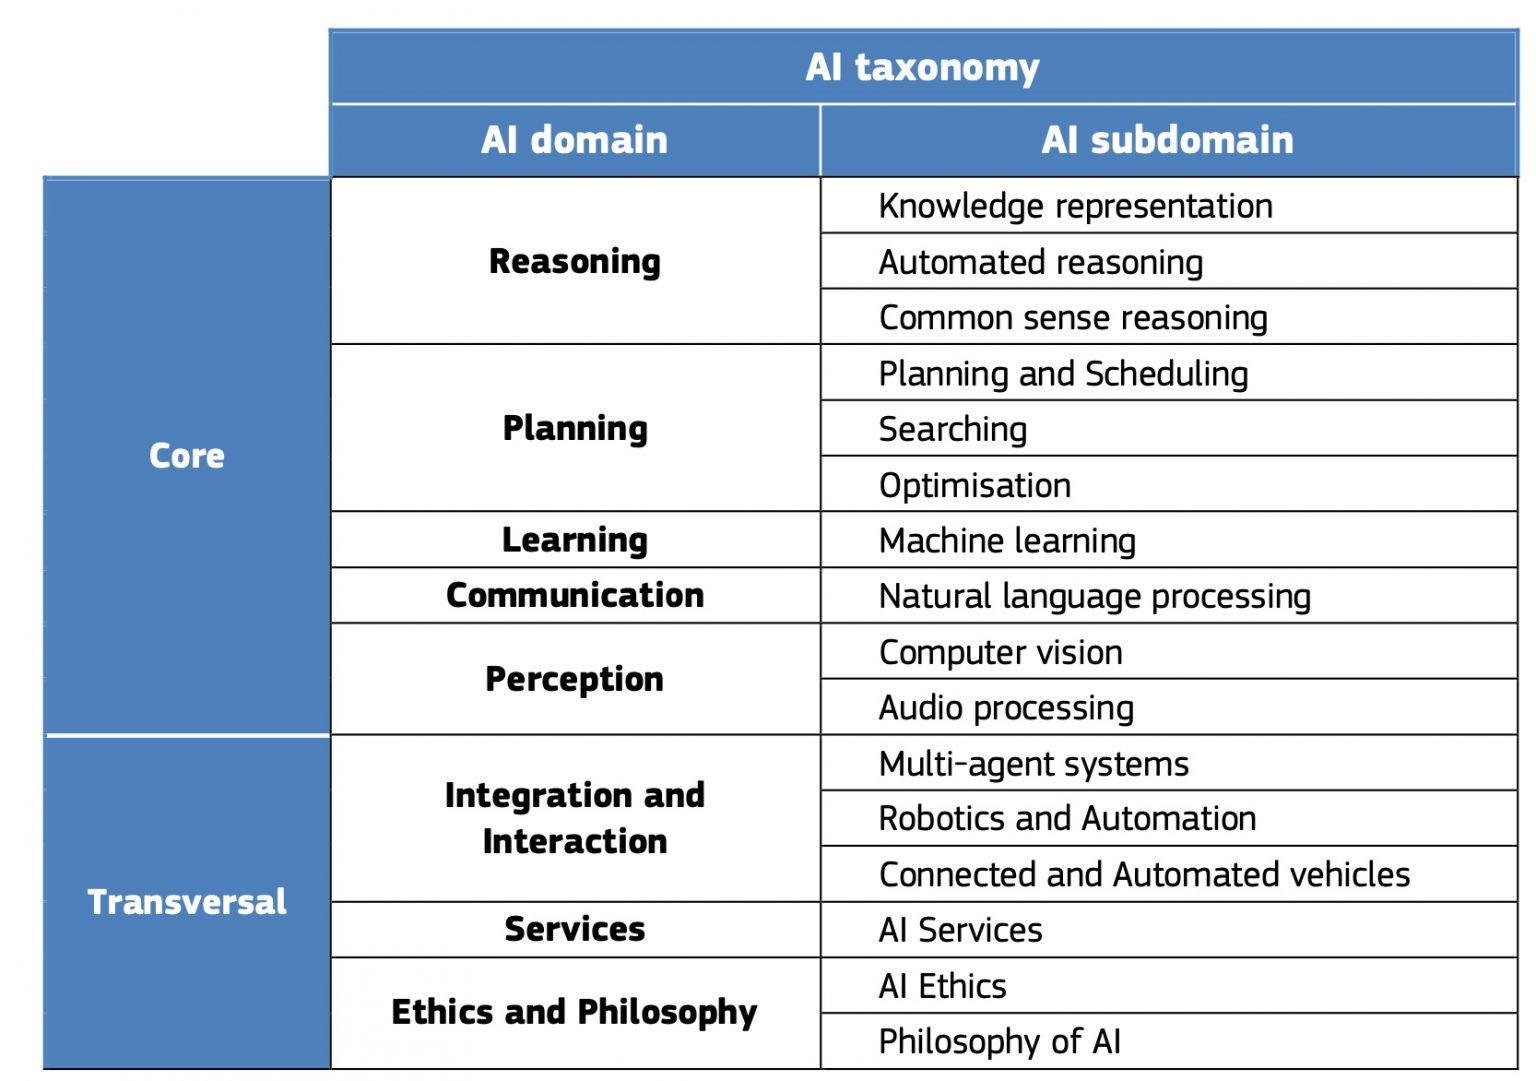
\includegraphics{Img/taxonomia.jpg}

}

\caption{Ramas}

\end{figure}%

Esta imagen presenta una \textbf{taxonomía de la Inteligencia Artificial
(IA)}, organizada en dominios y subdominios, que abarca tanto aspectos
\textbf{centrales (Core)} como \textbf{transversales (Transversal)} de
la IA. Aquí te explico cada sección:

\subsection{Dominio Central (Core):}\label{dominio-central-core}

Estos son los fundamentos o los componentes clave de la IA, que abarcan
desde cómo razona una máquina hasta cómo percibe e interactúa con el
mundo.

\begin{enumerate}
\def\labelenumi{\arabic{enumi}.}
\tightlist
\item
  \textbf{Reasoning (Razonamiento)}:

  \begin{itemize}
  \tightlist
  \item
    \textbf{Knowledge Representation}: Representación del conocimiento.
    Se refiere a cómo una máquina organiza y almacena la información de
    manera que pueda usarla para tomar decisiones o resolver problemas.
  \item
    \textbf{Automated Reasoning}: Razonamiento automatizado. La
    capacidad de la IA para derivar conclusiones y resolver problemas
    complejos basados en las reglas y el conocimiento almacenado.
  \item
    \textbf{Common Sense Reasoning}: Razonamiento de sentido común. La
    IA intenta razonar como lo haría una persona, utilizando
    conocimientos que los humanos damos por sentado, pero que las
    máquinas deben aprender o codificar.
  \end{itemize}
\item
  \textbf{Planning (Planificación)}:

  \begin{itemize}
  \tightlist
  \item
    \textbf{Planning and Scheduling}: Planificación y programación. La
    capacidad de la IA para organizar tareas o recursos en función de
    objetivos, optimizando tiempos y recursos.
  \item
    \textbf{Searching}: Búsqueda. IA encuentra soluciones a problemas o
    información relevante entre un conjunto de opciones.
  \item
    \textbf{Optimisation}: Optimización. Aquí la IA busca la mejor
    solución entre múltiples alternativas, ajustando variables para
    obtener el mejor rendimiento o eficiencia.
  \end{itemize}
\item
  \textbf{Learning (Aprendizaje)}:

  \begin{itemize}
  \tightlist
  \item
    \textbf{Machine Learning}: Aprendizaje automático. Esta es la
    capacidad de las máquinas para aprender a partir de datos sin ser
    programadas explícitamente para cada tarea. Es una de las áreas más
    destacadas y utilizadas en la IA actual.
  \end{itemize}
\item
  \textbf{Communication (Comunicación)}:

  \begin{itemize}
  \tightlist
  \item
    \textbf{Natural Language Processing}: Procesamiento del lenguaje
    natural. La IA comprende, interpreta y genera lenguaje humano,
    facilitando la interacción entre humanos y máquinas mediante el
    habla o el texto.
  \end{itemize}
\item
  \textbf{Perception (Percepción)}:

  \begin{itemize}
  \tightlist
  \item
    \textbf{Computer Vision}: Visión por computadora. La IA percibe el
    mundo visualmente, analizando imágenes o videos para detectar
    patrones, objetos o reconocer caras.
  \item
    \textbf{Audio Processing}: Procesamiento de audio. Similar a la
    visión por computadora, pero en este caso, la IA procesa y entiende
    sonidos, como la voz o música.
  \end{itemize}
\end{enumerate}

\subsection{Dominio Transversal:}\label{dominio-transversal}

Estas áreas complementan los dominios centrales, ofreciendo integración,
interacción y aspectos filosóficos o éticos.

\begin{enumerate}
\def\labelenumi{\arabic{enumi}.}
\tightlist
\item
  \textbf{Integration and Interaction (Integración e Interacción)}:

  \begin{itemize}
  \tightlist
  \item
    \textbf{Multi-agent Systems}: Sistemas multiagente. Conjunto de IA
    que trabajan juntas, colaborando o compitiendo para resolver
    problemas más complejos.
  \item
    \textbf{Robotics and Automation}: Robótica y automatización. Integra
    la IA con robots y sistemas automatizados para realizar tareas
    físicas, como ensamblar productos en fábricas.
  \item
    \textbf{Connected and Automated Vehicles}: Vehículos conectados y
    automatizados. Implica el uso de IA para controlar vehículos
    autónomos y conectados que operan sin intervención humana.
  \end{itemize}
\item
  \textbf{Services (Servicios)}:

  \begin{itemize}
  \tightlist
  \item
    \textbf{AI Services}: Servicios de IA. Herramientas y plataformas
    basadas en IA que las empresas y personas pueden utilizar para
    resolver problemas o mejorar procesos (por ejemplo, asistentes
    virtuales, análisis predictivos).
  \end{itemize}
\item
  \textbf{Ethics and Philosophy (Ética y Filosofía)}:

  \begin{itemize}
  \tightlist
  \item
    \textbf{AI Ethics}: Ética de la IA. Se ocupa de las cuestiones
    éticas relacionadas con el uso y el desarrollo de la IA, como la
    privacidad, la equidad y el impacto social.
  \item
    \textbf{Philosophy of AI}: Filosofía de la IA. Reflexiones más
    profundas sobre el papel de la IA en la sociedad y qué significa
    para las máquinas tener inteligencia similar a la humana.
  \end{itemize}
\end{enumerate}

\subsection{Resumen:}\label{resumen}

La taxonomía de la IA presentada en esta imagen divide los conceptos
fundamentales en dominios que abarcan \textbf{razonamiento},
\textbf{planificación}, \textbf{aprendizaje}, \textbf{comunicación} y
\textbf{percepción}. Estos conceptos son claves para entender cómo la IA
interactúa y aprende del mundo. Los dominios transversales complementan
estas capacidades con aspectos como la \textbf{integración}, los
\textbf{servicios de IA} y las \textbf{cuestiones éticas}, que son
fundamentales para asegurar un uso responsable y eficaz de la
inteligencia artificial en el mundo real.

\section{IA Simbólica}\label{ia-simbuxf3lica}

La Inteligencia Artificial Simbólica es un enfoque de la IA que se basa
en representar el conocimiento y el razonamiento a través de símbolos y
reglas lógicas. En lugar de aprender a partir de datos como ocurre en el
Machine Learning, la IA simbólica funciona siguiendo un conjunto de
instrucciones predefinidas para resolver problemas o tomar decisiones.
En este sistema, los programadores crean reglas claras que la máquina
debe seguir, y la IA utiliza estas reglas para tomar decisiones basadas
en relaciones lógicas de ``si-entonces'' o ``condiciones''.

Por ejemplo, en una maquiladora donde se ensamblan componentes
electrónicos, la IA simbólica puede controlar la temperatura de las
máquinas o la calidad de los productos sin margen de error, gracias a
sus reglas fijas. Este enfoque es ideal para tareas donde no hay mucha
variabilidad, y se requiere cumplir con estrictos parámetros de
producción.

Este enfoque es como una receta: todo está previamente determinado, y la
máquina sigue los pasos sin desviarse. Por ejemplo, un sistema de IA
simbólica podría estar programado para diagnosticar fallos en una
máquina si ciertas condiciones, como la temperatura o la vibración,
exceden los límites establecidos. Cada condición está claramente
definida, y la IA actúa según las reglas sin necesidad de adaptarse o
aprender nuevas formas de solucionar el problema.

La IA simbólica es particularmente útil en entornos donde los procesos
son repetitivos o bien estructurados. En la maquiladora, se usa en casos
como el control de calidad basado en reglas predefinidas o la gestión de
tiempos de producción. Aunque no es flexible como el Machine Learning,
la IA simbólica es extremadamente precisa y eficiente cuando se trata de
ejecutar tareas que siguen un patrón fijo y bien entendido.

La IA Simbólica se utiliza en situaciones donde las reglas y
procedimientos están claramente definidos y son consistentes. Este
enfoque es ideal para procesos repetitivos o controlados, donde se
pueden establecer reglas lógicas y secuencias de pasos que la máquina
debe seguir sin necesidad de aprender o adaptarse. En estos casos, la IA
simbólica es altamente confiable porque sigue estrictamente las
instrucciones que se le proporcionan. Por ejemplo, en una maquiladora,
el ensamblaje de piezas con pasos fijos o la programación de tiempos de
producción puede ser gestionado eficientemente por IA simbólica, ya que
las condiciones no varían mucho y las decisiones se toman en base a
reglas claras.

Además, la IA simbólica se usa en aplicaciones como sistemas expertos,
donde se requiere tomar decisiones basadas en conocimientos específicos,
como el diagnóstico de fallos de máquinas. Aquí, se definen reglas de
``si-entonces'' que guían la toma de decisiones: ``Si la temperatura del
motor sube más de 80°C, entonces apaga la máquina''. Aunque este enfoque
no es flexible ni aprende de los datos, es muy eficaz cuando los
parámetros y resultados son predecibles, y se necesita precisión sin
variaciones.

La IA simbólica se adapta mejor a contextos donde el entorno es estable,
los datos no cambian de manera dinámica, y las decisiones se pueden
programar de antemano. Por eso, en áreas de la maquila como control de
procesos, administración de turnos o mantenimiento bajo condiciones
estándar, sigue siendo una opción confiable y eficiente.

Este tipo de robot es un ejemplo de \textbf{IA Simbólica}, porque sigue
un conjunto de reglas claras para completar la tarea. Cada paso está
definido de manera precisa, y el robot simplemente sigue las
instrucciones. Si la receta no cambia, el robot siempre hará el pastel
de la misma manera, una y otra vez. No necesita aprender ni adaptarse
porque todo está programado de antemano.

En la industria maquiladora, este tipo de IA puede ser útil para tareas
repetitivas como ensamblar piezas, donde las reglas del proceso son
claras y no cambian con el tiempo. \textbf{Imagina} una línea de
producción donde una máquina ensambla componentes electrónicos: coloca
una pieza aquí, ajusta un tornillo allá. Siempre que las instrucciones
sean las mismas, la IA simbólica funciona perfectamente.

Sin embargo, no todos los procesos en una maquiladora son tan
predecibles. Aquí es donde entra el Machine Learning. En lugar de seguir
reglas fijas, el Machine Learning es como el chef aprendiz: aprende y
mejora con el tiempo a medida que recopila más información. En la
maquila, esto es útil en situaciones donde hay variabilidad, como
ajustes en las máquinas para mejorar la calidad o la predicción de
fallos en los equipos. A medida que las máquinas recolectan datos
durante la producción, el Machine Learning puede optimizar los procesos
y hacer ajustes para aumentar la eficiencia

\subsubsection{Ejemplo: IA Simbólica con Receta de
Cocina}\label{ejemplo-ia-simbuxf3lica-con-receta-de-cocina}

\textbf{Imagina} que le das a un robot una receta detallada para hacer
un pastel. Le das instrucciones específicas como: 1. Mezcla 200 gramos
de harina con 100 gramos de azúcar. 2. Añade dos huevos y bate la mezcla
por 5 minutos. 3. Coloca la mezcla en el horno a 180°C durante 30
minutos.

\subsubsection{Ejemplo: Machine Learning como Chef
Aprendiz}\label{ejemplo-machine-learning-como-chef-aprendiz}

Ahora, \textbf{imagina} que en lugar de seguir siempre la misma receta,
tienes un robot que quiere convertirse en un chef experto. En lugar de
seguir instrucciones precisas, este robot observa a diferentes cocineros
haciendo pasteles y aprende de sus técnicas. Tal vez nota que algunos
cocineros usan más azúcar, otros agregan ingredientes extra como
vainilla, y algunos hornean el pastel por más tiempo dependiendo del
tipo de horno. El robot comienza a \textbf{aprender} que, dependiendo de
ciertos factores, puede ajustar la receta para hacer el mejor pastel
posible.

Este es un ejemplo de \textbf{Machine Learning}, donde la IA no sigue
reglas predefinidas, sino que aprende a partir de los datos que
recopila. En lugar de seguir la misma receta siempre, el robot adapta la
receta según los datos que ha recopilado (temperatura ambiente, tipo de
ingredientes, preferencias de sabor, etc.).

En una maquiladora, un sistema de \textbf{Machine Learning} puede hacer
lo mismo con tus datos de producción. \textbf{Imagina} que tienes una
máquina que fabrica piezas de plástico, y las condiciones varían según
la temperatura o el tipo de material que estás utilizando. Un sistema de
Machine Learning puede observar estos factores y ajustar automáticamente
los parámetros de la máquina para obtener el mejor rendimiento. Si nota
que la calidad del producto disminuye cuando la temperatura sube más de
cierto punto, aprenderá a ajustar la temperatura para mantener la
calidad.

\subsubsection{Comparando los Enfoques}\label{comparando-los-enfoques}

\begin{itemize}
\item
  \textbf{IA Simbólica}: Es como el robot que sigue una receta fija.
  Funciona bien en situaciones donde las reglas son claras y no cambian
  mucho. Esto es útil en procesos repetitivos como el ensamblaje en una
  maquila, donde los pasos son los mismos cada día.
\item
  \textbf{Machine Learning}: Es como el chef aprendiz. En lugar de
  seguir reglas fijas, aprende y mejora con el tiempo a medida que
  recopila más información. En la maquila, esto es útil en situaciones
  donde hay variabilidad, como ajustes en las máquinas para mejorar la
  calidad o la predicción de fallos en los equipos.
\end{itemize}

\subsubsection{Ejemplo: IA en el Control de
Calidad}\label{ejemplo-ia-en-el-control-de-calidad}

\textbf{Imagina} que en tu maquila produces miles de piezas cada día, y
necesitas asegurarte de que todas cumplan con los estándares de calidad.
En lugar de tener a una persona revisando cada pieza (lo cual puede ser
lento y propenso a errores), podrías usar \textbf{IA Simbólica} o
\textbf{Machine Learning}.

\begin{itemize}
\item
  Con \textbf{IA Simbólica}, podrías programar una máquina para revisar
  cada pieza siguiendo reglas específicas. Por ejemplo: ``Si la pieza
  tiene más de 0.5 mm de desviación, recházala''. Esto es eficiente,
  pero solo funciona para detectar errores simples.
\item
  Con \textbf{Machine Learning}, podrías entrenar a una máquina para
  detectar patrones más complejos. El sistema podría aprender a
  reconocer qué tipo de defectos aparecen con mayor frecuencia y, con el
  tiempo, predecir dónde y cuándo es más probable que aparezcan
  defectos, ajustando la producción en consecuencia. Podría incluso
  aprender de nuevos datos para mejorar la precisión a lo largo del
  tiempo.
\end{itemize}

\subsubsection{Reflexión Final: Bajar la IA a lo
Práctico}\label{reflexiuxf3n-final-bajar-la-ia-a-lo-pruxe1ctico}

La IA, en su forma más simple, es una herramienta que ayuda a las
máquinas a hacer tareas que normalmente haría un humano, pero con mayor
precisión y eficiencia. No necesitas ser un experto para empezar a
entender cómo puede mejorar tu maquila. Lo importante es reconocer que
hay dos formas principales en que la IA puede ayudarte:
\textbf{siguiendo reglas fijas (IA Simbólica)} o \textbf{aprendiendo de
los datos (Machine Learning)}. Y aunque los conceptos técnicos puedan
sonar complicados, los beneficios prácticos son claros: más eficiencia,
menos errores, y una producción más ágil y adaptada a las necesidades
del día a día.

Al final del día, implementar IA en la maquila puede ser tan sencillo
como hacer un pastel siguiendo una receta, o tan avanzado como un chef
que mejora sus técnicas con cada plato que cocina. Lo importante es
saber cuál enfoque se adapta mejor a tus necesidades y empezar a
aprovecharlo para llevar tu operación al siguiente nivel. ¡A darle!s

\subsection{IA Simbólica: Conceptos Claros con Diagramas de
Flujo}\label{ia-simbuxf3lica-conceptos-claros-con-diagramas-de-flujo}

La Inteligencia Artificial Simbólica es un enfoque donde la IA opera
basándose en reglas predefinidas, es decir, un conjunto de condiciones
lógicas establecidas por programadores que guían las acciones de la
máquina. A continuación, te explico cómo se pueden usar elementos clave
como los diagramas de flujo para implementar IA simbólica de manera
clara y estructurada en un entorno práctico, como una maquiladora.

\textbf{Concepto de IA Simbólica}

La IA simbólica se fundamenta en reglas lógicas que siguen el esquema de
``si-entonces'' (if-then). Esto significa que la máquina ejecutará una
acción dependiendo de si una condición específica se cumple o no.

Por ejemplo:

\begin{itemize}
\tightlist
\item
  Condición: Si la temperatura de la máquina supera los 80°C, entonces
  envía una alerta.
\item
  Condición 2: Si el nivel de stock de un producto es menor a 100
  unidades, entonces genera una orden de compra.
\end{itemize}

Este tipo de razonamiento es ideal para tareas automatizadas y procesos
repetitivos donde las condiciones son predecibles.

\textbf{Elementos Clave para Implementar IA Simbólica}

\begin{itemize}
\tightlist
\item
  \textbf{Diagrama de Flujo}
\end{itemize}

Un diagrama de flujo es una representación gráfica de un proceso. En el
caso de la IA simbólica, se puede utilizar para ilustrar cómo las reglas
lógicas guían el comportamiento del sistema.

\emph{Ejemplo de un diagrama de flujo para IA simbólica:}

\begin{itemize}
\tightlist
\item
  Inicio: El sistema comienza a monitorear la temperatura de la máquina.
\item
  Condición 1: ¿La temperatura es mayor a 80°C?

  \begin{itemize}
  \tightlist
  \item
    Sí: Detener la máquina y enviar alerta al supervisor (acción A).
  \item
    No: Continuar monitoreando (acción B).
  \end{itemize}
\item
  Condición 2: ¿El nivel de stock es menor a 100 unidades?

  \begin{itemize}
  \tightlist
  \item
    Sí: Generar orden de compra automáticamente (acción C).
  \item
    No: Seguir con el proceso de producción (acción D).
  \end{itemize}
\end{itemize}

En este flujo, cada decisión está basada en una condición clara que
lleva a una acción específica. Esto es exactamente cómo funciona la IA
simbólica, ya que sigue reglas de este tipo sin necesidad de aprender o
ajustarse con el tiempo.

\textbf{Ejemplo Aplicado: Sistema de Control de Inventario}

\begin{itemize}
\item
  Escenario: Imagina que en tu maquila tienes un sistema de control de
  inventario. Este sistema necesita generar automáticamente una orden de
  compra cuando el nivel de stock de cierto material cae por debajo de
  un umbral.
\item
  Condiciones Predefinidas:

  \begin{itemize}
  \tightlist
  \item
    Regla 1: Si el stock es menor a 50 unidades, entonces enviar alerta.
  \item
    Regla 2: Si el stock es menor a 10 unidades, generar automáticamente
    una orden de compra.
  \end{itemize}
\item
  Diagrama de Flujo para la IA Simbólica del Inventario:

  \begin{itemize}
  \tightlist
  \item
    Inicio: El sistema verifica el nivel de stock.
  \item
    Condición 1: ¿El stock es menor a 50?

    \begin{itemize}
    \tightlist
    \item
      Sí: Envía alerta al responsable de inventarios.
    \item
      No: Continuar monitoreando.
    \end{itemize}
  \item
    Condición 2: ¿El stock es menor a 10?

    \begin{itemize}
    \tightlist
    \item
      Sí: Generar orden de compra automáticamente.
    \item
      No: Mantener el inventario.
    \end{itemize}
  \end{itemize}
\end{itemize}

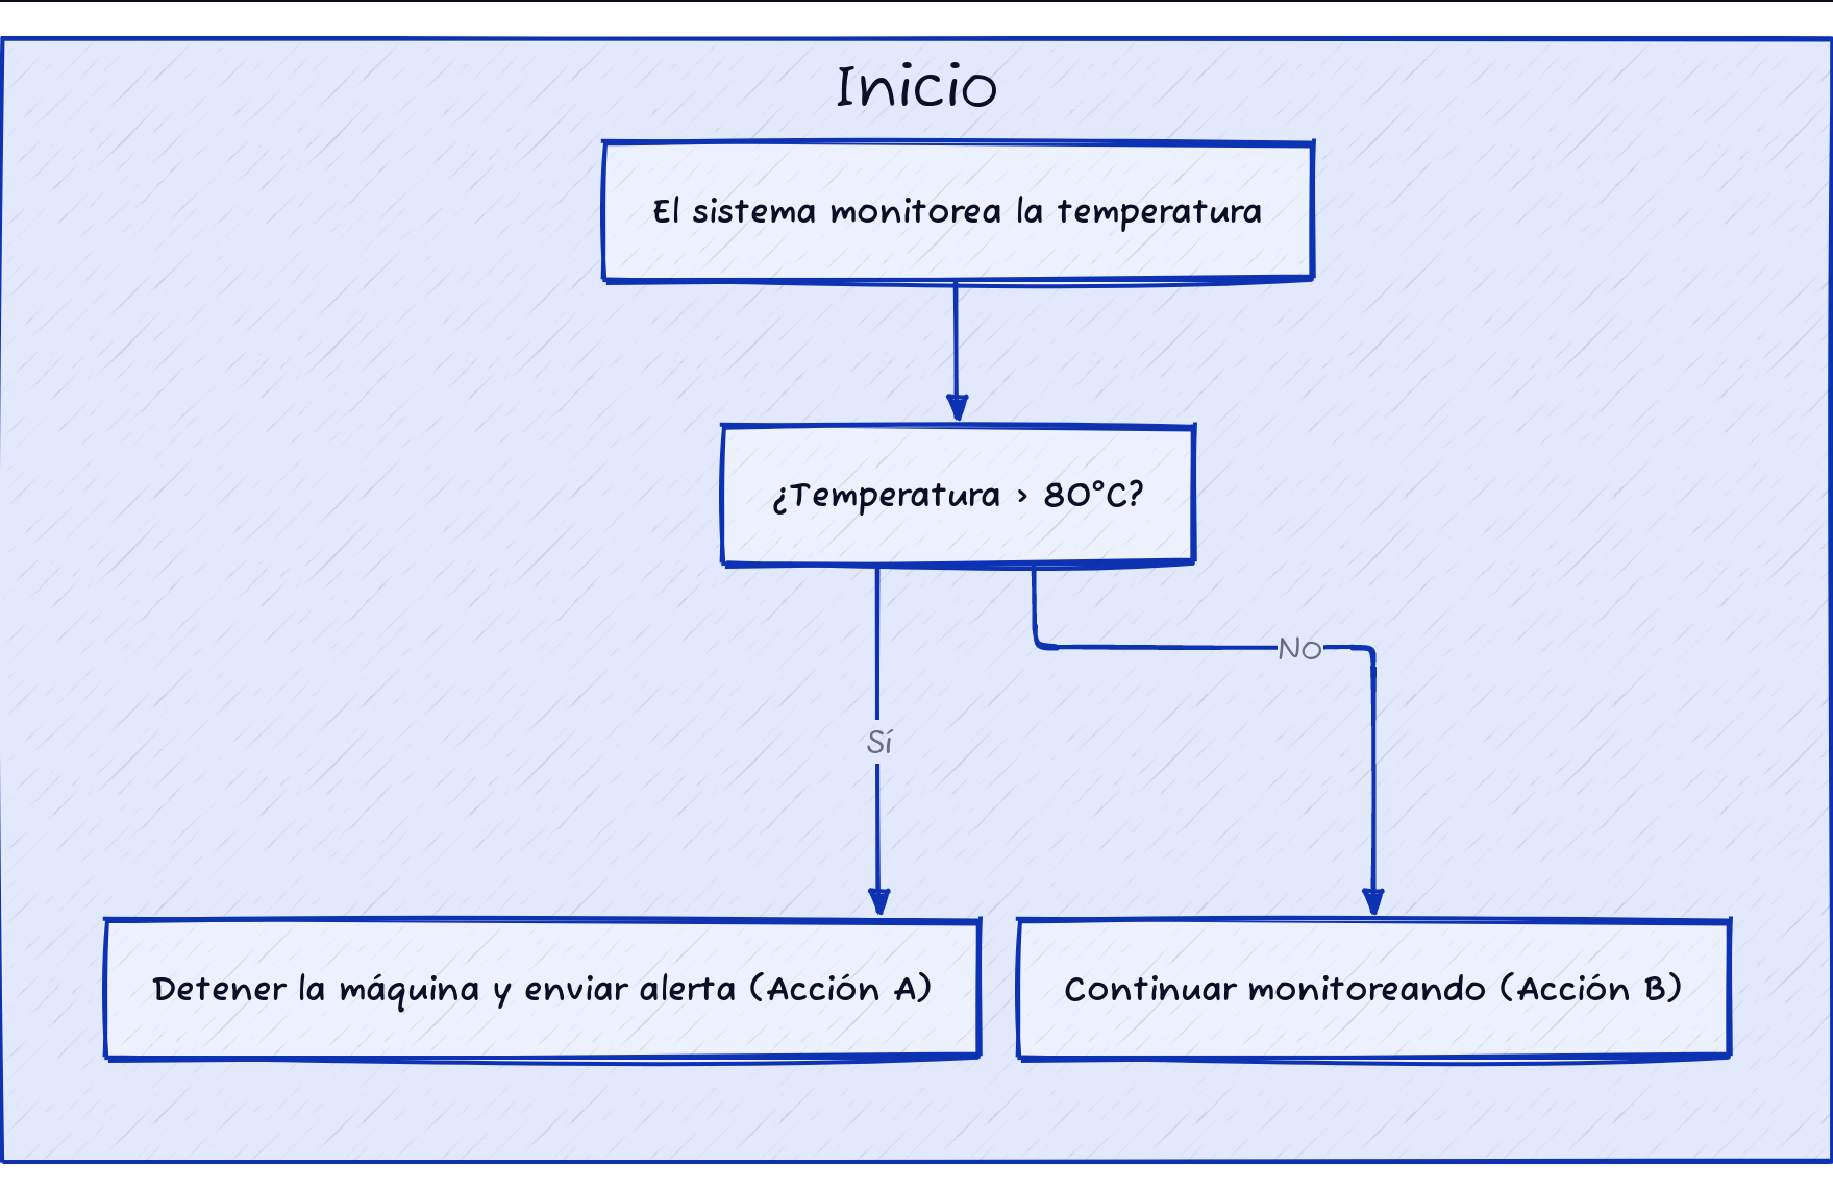
\includegraphics[width=1\textwidth,height=\textheight]{index_files/mediabag/diagram-1.pdf}

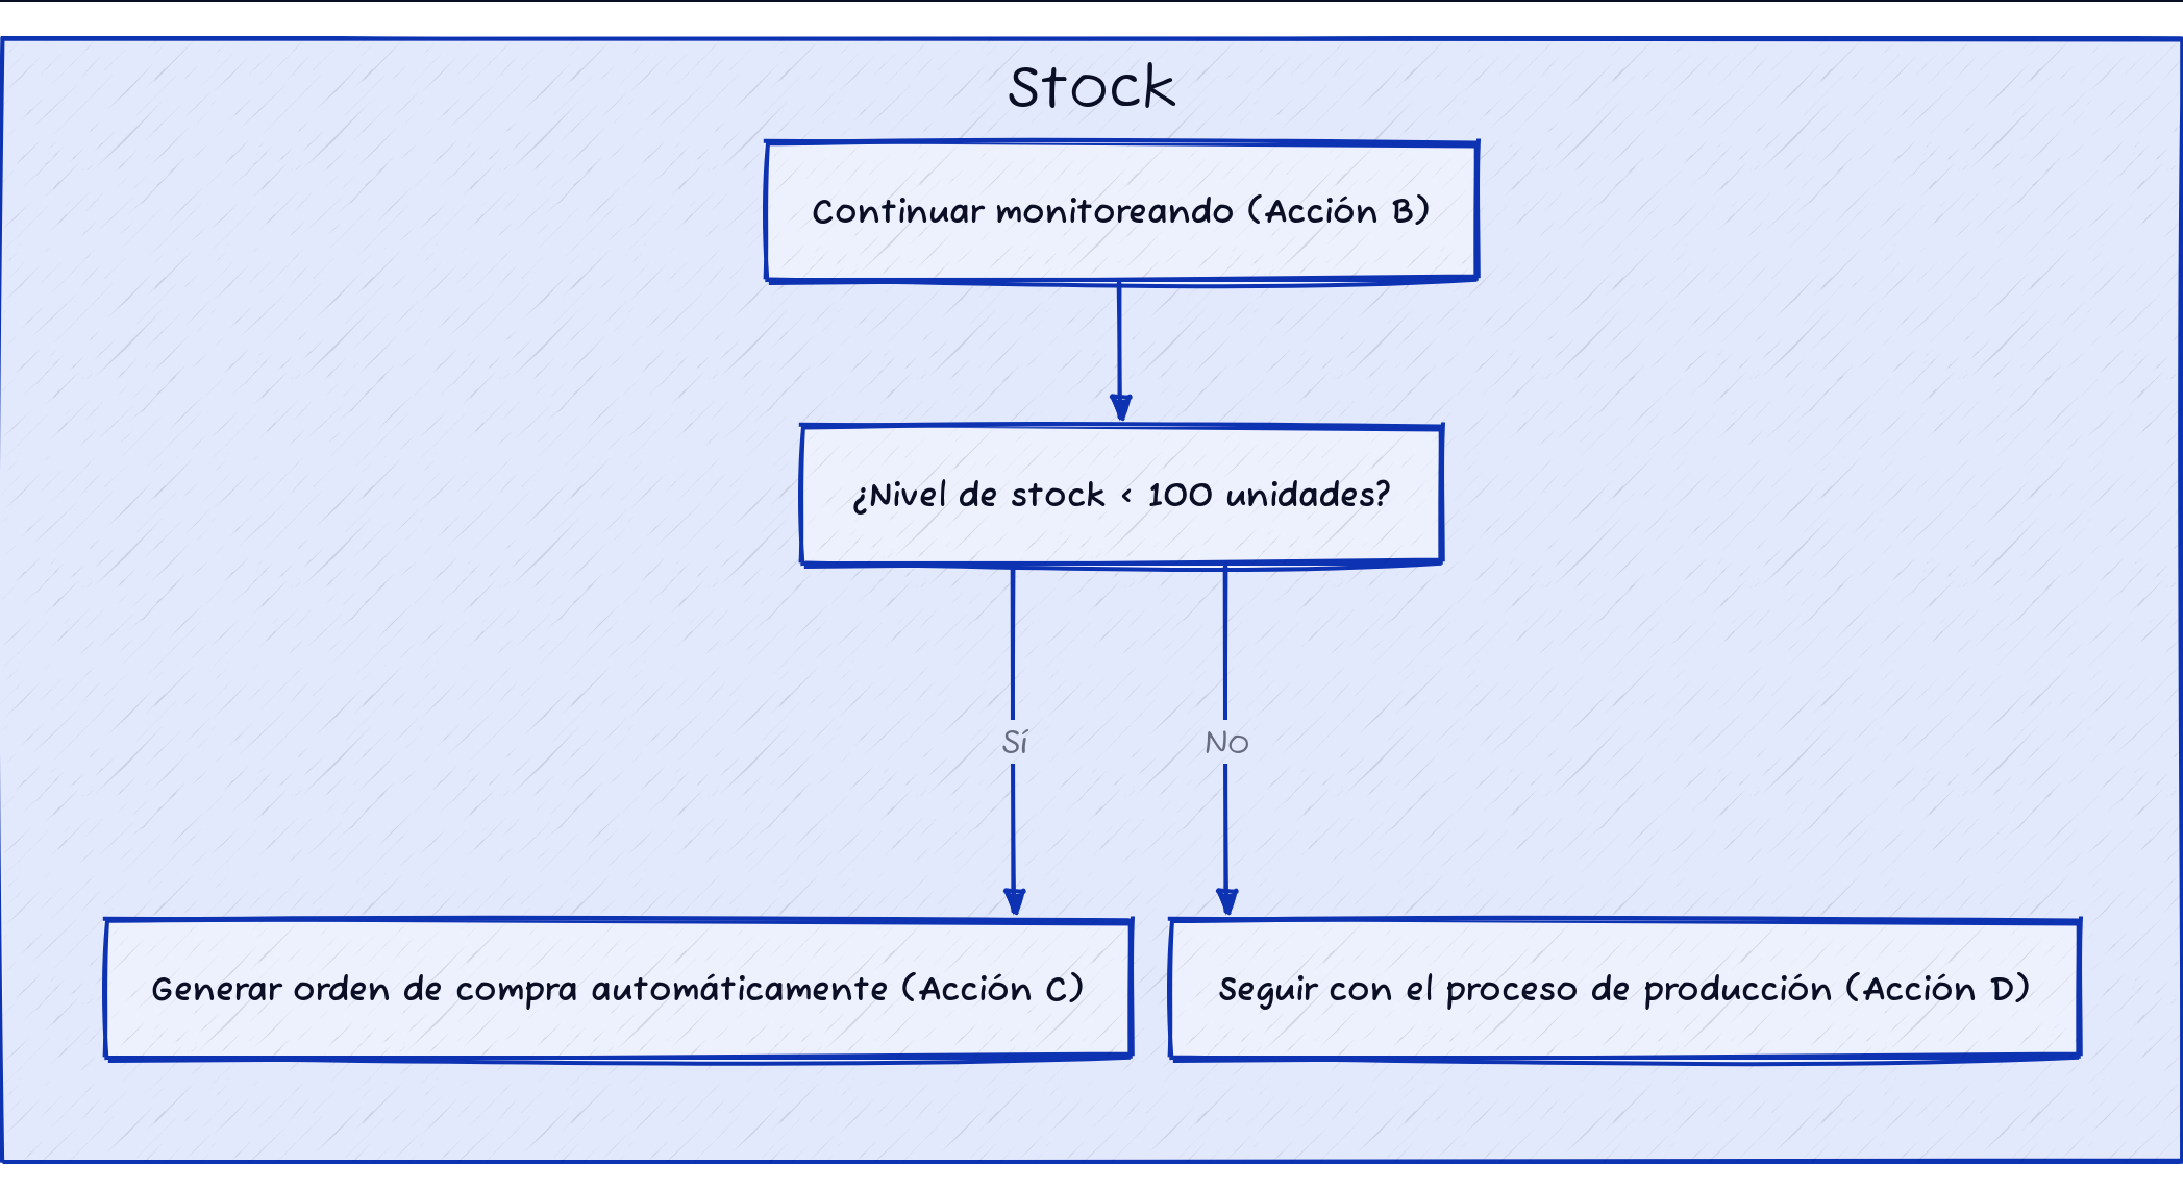
\includegraphics[width=1\textwidth,height=\textheight]{index_files/mediabag/diagram-2.pdf}

\textbf{Referencia:}

\begin{itemize}
\tightlist
\item
  \textbf{Russell, S. J., \& Norvig, P. (2020). \emph{Artificial
  Intelligence: A Modern Approach (4th ed.)}. Pearson.} Este libro es
  una referencia clásica en el campo de la Inteligencia Artificial y
  proporciona una base sólida para comprender los diferentes enfoques,
  incluyendo la IA simbólica. ¡Entiendo lo que estás buscando! Vamos a
  darle un enfoque más \textbf{didáctico} y estructurado, usando listas
  y secciones que faciliten la lectura y el entendimiento, mientras
  mantenemos el mismo contenido. Aquí te dejo la nueva versión:
\end{itemize}

\subsection{Capítulo: Las Ventajas de la IA Simbólica: El Primer Paso
Hacia la
Automatización}\label{capuxedtulo-las-ventajas-de-la-ia-simbuxf3lica-el-primer-paso-hacia-la-automatizaciuxf3n}

En cualquier organización, como una maquiladora, el conocimiento
operativo a menudo está centralizado en una persona o en archivos que
pocos pueden entender. Esto puede ser un riesgo significativo, ya que la
dependencia de personas específicas o de sistemas manuales, como
archivos de Excel, puede frenar la eficiencia de los procesos. La
\textbf{IA Simbólica} ofrece una solución práctica para automatizar y
descentralizar este conocimiento, permitiendo que los procesos se
formalicen y ejecuten de manera coherente sin depender de un solo
individuo.

La IA Simbólica funciona mediante reglas predefinidas que permiten a las
máquinas tomar decisiones basadas en condiciones claras, como el clásico
``si-entonces'' (if-then). A continuación, exploramos las ventajas de la
IA Simbólica y por qué representa el primer paso esencial hacia la
automatización inteligente en una maquiladora.

\subsubsection{¿Por qué Usar IA Simbólica en Tu
Maquiladora?}\label{por-quuxe9-usar-ia-simbuxf3lica-en-tu-maquiladora}

\begin{enumerate}
\def\labelenumi{\arabic{enumi}.}
\item
  \textbf{Automatización de Tareas Repetitivas}\\
  La IA Simbólica es ideal para procesos donde las condiciones no
  cambian mucho y las reglas pueden definirse claramente. Esto incluye
  tareas como:

  \begin{itemize}
  \tightlist
  \item
    \textbf{Gestión de Inventarios}: Automatizar las órdenes de compra
    cuando los niveles de stock caen por debajo de un umbral.
  \item
    \textbf{Mantenimiento Preventivo}: Detener máquinas o enviar alertas
    cuando ciertos parámetros, como la temperatura, superan los límites
    seguros.
  \end{itemize}
\item
  \textbf{Descentralización del Conocimiento}\\
  Muchas veces, los procesos clave de la empresa dependen de una sola
  persona o de archivos mal organizados. Con la IA Simbólica, la lógica
  del negocio se transfiere a reglas claras y automatizadas, evitando
  que el conocimiento esté centralizado en una sola fuente. Esto reduce
  riesgos y asegura la continuidad del negocio, incluso si el personal
  cambia.
\item
  \textbf{Claridad y Transparencia con Diagramas de Flujo}\\
  Un gran beneficio de la IA Simbólica es la \textbf{visualización de
  procesos} mediante \textbf{diagramas de flujo}. Estos diagramas
  permiten a todos entender cómo se toman las decisiones dentro del
  sistema, lo que facilita la comunicación y mejora la colaboración
  entre departamentos. Un diagrama de flujo podría verse algo así:

  \begin{itemize}
  \tightlist
  \item
    \textbf{Inicio}: El sistema comienza a monitorear la temperatura de
    la máquina.
  \item
    \textbf{Condición 1}: ¿La temperatura es mayor a 80°C?

    \begin{itemize}
    \tightlist
    \item
      \textbf{Sí}: Detener la máquina y enviar una alerta al supervisor.
    \item
      \textbf{No}: Continuar monitoreando.
    \end{itemize}
  \item
    \textbf{Condición 2}: ¿El nivel de stock es menor a 100 unidades?

    \begin{itemize}
    \tightlist
    \item
      \textbf{Sí}: Generar una orden de compra automáticamente.
    \item
      \textbf{No}: Continuar el proceso de producción.
    \end{itemize}
  \end{itemize}

  \textbf{Conclusión:} Este enfoque permite que todos los miembros del
  equipo, desde los operadores hasta los supervisores, entiendan
  claramente cómo se toman las decisiones en cada etapa del proceso.
\end{enumerate}

\subsubsection{Ejemplo Práctico: Sistema de Control de
Inventario}\label{ejemplo-pruxe1ctico-sistema-de-control-de-inventario}

\textbf{Escenario:}\\
Imagina que en tu maquiladora manejas grandes cantidades de inventario y
necesitas automatizar el proceso de reabastecimiento. Tradicionalmente,
un encargado del almacén revisa manualmente los niveles de stock y crea
órdenes de compra cuando se está quedando sin material. Este proceso
manual puede ser ineficiente, propenso a errores y muy dependiente de
una sola persona.

\textbf{Con IA Simbólica, este proceso puede automatizarse fácilmente
mediante las siguientes reglas:}

\begin{itemize}
\tightlist
\item
  \textbf{Condición 1}: Si el stock es menor a 50 unidades, enviar una
  alerta.
\item
  \textbf{Condición 2}: Si el stock es menor a 10 unidades, generar
  automáticamente una orden de compra.
\end{itemize}

\textbf{Ventajas para el Negocio:}

\begin{itemize}
\tightlist
\item
  \textbf{Reducción de errores humanos}: No dependerás de que alguien se
  acuerde de revisar los niveles de stock, ya que el sistema lo hará por
  ti.
\item
  \textbf{Eficiencia mejorada}: Al automatizar las órdenes de compra, se
  eliminan retrasos que podrían detener la producción.
\item
  \textbf{Descentralización del proceso}: No importa si el encargado de
  inventarios está presente o no, el sistema seguirá funcionando
  automáticamente.
\end{itemize}

\subsubsection{Un mito Famoso en la Comunidad de
Desarrolladores}\label{un-mito-famoso-en-la-comunidad-de-desarrolladores}

Aquí es donde entra un meme que muchos desarrolladores de software
comparten en tono de broma: el meme del programador que, después de
realizar una tarea manual y repetitiva mil veces, finalmente decide
crear un programa para automatizar esa tarea.

\begin{figure}[H]

{\centering 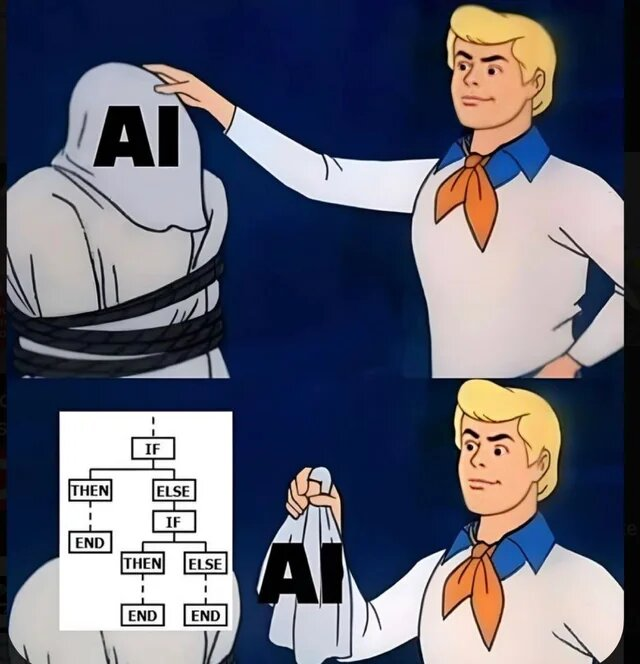
\includegraphics{Img/ia.jpg}

}

\caption{Meme}

\end{figure}%

La IA Simbólica es, en esencia, esa ``solución'' para las tareas
repetitivas en la maquiladora. En lugar de depender de que alguien haga
las mismas tareas una y otra vez, se implementan reglas claras que
permiten que las máquinas lo hagan de forma automática. \textbf{Imagina
la diferencia en eficiencia cuando ya no dependes de una persona que
tenga que hacer manualmente cada ajuste o revisión.}

\subsubsection{Ventajas Principales de la IA Simbólica para Tu
Maquiladora}\label{ventajas-principales-de-la-ia-simbuxf3lica-para-tu-maquiladora}

Vamos a resumir las principales ventajas en una lista clara:

\begin{enumerate}
\def\labelenumi{\arabic{enumi}.}
\tightlist
\item
  \textbf{Automatización de procesos repetitivos}: Perfecto para tareas
  donde las reglas no cambian con frecuencia.
\item
  \textbf{Descentralización del conocimiento}: Evita que el conocimiento
  esté retenido por una sola persona o en un archivo difícil de manejar.
\item
  \textbf{Eficiencia y precisión}: Reduce los errores humanos y asegura
  que las tareas se realicen de manera uniforme.
\item
  \textbf{Escalabilidad}: Es fácil modificar las reglas si el proceso o
  las condiciones cambian, haciendo la solución flexible y adaptable.
\item
  \textbf{Mejor colaboración}: Los diagramas de flujo y las reglas son
  fácilmente comprensibles para todos en la organización, facilitando la
  integración entre equipos.
\end{enumerate}

\subsubsection{¿Por Qué Empezar con la IA
Simbólica?}\label{por-quuxe9-empezar-con-la-ia-simbuxf3lica}

Si tu maquila aún no ha dado el salto hacia la automatización, la IA
Simbólica es la mejor opción para comenzar. \textbf{Es simple de
implementar, fácil de entender y muy efectiva} para automatizar procesos
que sigan reglas claras. A medida que tu negocio crezca, puedes seguir
construyendo sobre esta base, añadiendo más complejidad y flexibilidad,
pero el primer paso es crucial para reducir la dependencia de sistemas
manuales y asegurar que el conocimiento esté disponible para todos.

\subsubsection{Conclusión: El Primer Paso Hacia la Automatización
Inteligente}\label{conclusiuxf3n-el-primer-paso-hacia-la-automatizaciuxf3n-inteligente}

La \textbf{IA Simbólica} es un paso esencial para que tu maquila avance
hacia la automatización y la descentralización del conocimiento. Al
establecer reglas claras y estructuradas, respaldadas por diagramas de
flujo, puedes asegurar que todos los procesos se realicen de manera
eficiente, sin depender de una sola persona o archivo.

Si aún operas en un entorno donde la lógica de negocio está en manos de
unos pocos o donde los procesos manuales dominan, la IA Simbólica es tu
punto de partida ideal. \textbf{Es el primer paso hacia un futuro más
ágil, eficiente y colaborativo.}

\subsection{Perfil para Trabajar con IA Simbólica en una
Maquiladora}\label{perfil-para-trabajar-con-ia-simbuxf3lica-en-una-maquiladora}

Para implementar y gestionar la \textbf{IA Simbólica} en una
maquiladora, se necesita un perfil multidisciplinario que combine
habilidades técnicas con un profundo conocimiento de los procesos
industriales. A continuación, te describo el perfil ideal para alguien
que trabajará en la adopción y gestión de la IA simbólica en un entorno
de producción.

Lo importante es saber cuál enfoque se adapta mejor a tus necesidades y
empezar a aprovecharlo para llevar tu operación al siguiente nivel.

En los próximos capítulos, exploraremos más a fondo cómo estas
tecnologías están transformando cada rincón de las maquiladoras, desde
la automatización del control de calidad hasta la optimización de los
tiempos de producción. El siguiente paso es entender cómo implementar
estas tecnologías de manera efectiva y cuáles son los desafíos que
enfrentan las empresas en este proceso de digitalización.

\textbf{1. Conocimiento Técnico en Programación y Lógica}

Dado que la IA simbólica se basa en reglas predefinidas y condiciones
lógicas, es crucial que el candidato tenga sólidos conocimientos de
\textbf{programación} y \textbf{lógica de procesos}. Estos son algunos
de los requisitos técnicos:

\begin{itemize}
\tightlist
\item
  \textbf{Lenguajes de Programación}: Competencia en lenguajes de
  programación que permiten definir reglas y algoritmos, como
  \textbf{Python}, \textbf{C++}, o lenguajes específicos de
  automatización industrial (como \textbf{Ladder Logic} o
  \textbf{Structured Text} para PLCs).
\item
  \textbf{Experiencia en Sistemas de Automatización}: Conocimiento de
  sistemas SCADA o PLC (Controladores Lógicos Programables) que se
  utilizan ampliamente en entornos industriales.
\item
  \textbf{Manejo de Reglas Lógicas}: Habilidad para diseñar y gestionar
  reglas de ``si-entonces'' (if-then) y otros tipos de reglas lógicas
  que determinan el comportamiento de los sistemas de IA simbólica.
\item
  \textbf{Diagramas de Flujo}: Capacidad para diseñar, interpretar y
  modificar diagramas de flujo que describen el funcionamiento del
  sistema de IA simbólica.
\end{itemize}

\textbf{2. Conocimiento en Procesos Industriales}

Es fundamental que la persona tenga un buen entendimiento de los
procesos específicos de la \textbf{industria maquiladora}. Esto
permitirá al profesional identificar las áreas donde la IA simbólica
puede ser más útil y generar un mayor impacto en la eficiencia y
automatización de procesos.

\begin{itemize}
\tightlist
\item
  \textbf{Control de Calidad}: Comprender cómo funcionan los sistemas de
  control de calidad en la línea de producción y cómo la IA puede
  optimizar el proceso mediante reglas predefinidas para la detección de
  defectos.
\item
  \textbf{Gestión de Inventarios}: Saber cómo operan los sistemas de
  inventario y cómo las reglas lógicas pueden automatizar las órdenes de
  compra y el reabastecimiento.
\item
  \textbf{Mantenimiento de Máquinas}: Conocimiento sobre los ciclos de
  mantenimiento y cómo establecer reglas simbólicas para alertas y
  paradas preventivas.
\end{itemize}

\textbf{3. Habilidad para Diseñar Sistemas Basados en Reglas}

Una de las tareas más importantes de este perfil es diseñar y optimizar
las reglas que seguirá la IA simbólica. Esto requiere una capacidad para
crear reglas claras y efectivas que cubran todas las posibles
condiciones y escenarios que pueden presentarse en la maquiladora.

\begin{itemize}
\tightlist
\item
  \textbf{Diseño de Reglas Condicionales}: Capacidad para desarrollar un
  sistema de reglas eficiente, asegurándose de que todas las situaciones
  posibles estén cubiertas. Ejemplo: ``Si el nivel de vibración de una
  máquina supera el umbral X, entonces enviar una alerta.''
\item
  \textbf{Optimización de Procesos}: Habilidad para analizar y optimizar
  procesos mediante la creación de flujos lógicos claros, reduciendo
  tiempos muertos y aumentando la eficiencia de la producción.
\end{itemize}

\textbf{4. Experiencia en Implementación de Soluciones de IA Simbólica}

El candidato debe tener experiencia práctica en la implementación de
sistemas basados en IA simbólica, desde el diseño inicial hasta la
puesta en marcha y ajuste de reglas en entornos reales de producción.

\begin{itemize}
\tightlist
\item
  \textbf{Configuración e Integración}: Capacidad para configurar la IA
  simbólica en los sistemas existentes, integrando la tecnología con
  otras soluciones industriales como ERPs, SCADA, o sistemas de gestión
  de inventarios.
\item
  \textbf{Pruebas y Validación}: Habilidad para realizar pruebas y
  validar que las reglas y condiciones están funcionando de acuerdo con
  lo esperado, ajustando según sea necesario para mejorar la precisión
  del sistema.
\end{itemize}

\textbf{5. Competencias en Análisis de Datos}

Aunque la IA simbólica no aprende de los datos como el Machine Learning,
sigue siendo importante que el profesional pueda analizar datos
históricos o de producción para definir reglas de manera efectiva.

\begin{itemize}
\tightlist
\item
  \textbf{Analizar Patrones}: Capacidad para observar patrones en el
  comportamiento de las máquinas, en los tiempos de producción o en los
  niveles de inventario, que puedan traducirse en reglas lógicas.
\item
  \textbf{Generación de Reportes}: Habilidad para generar y analizar
  reportes de producción, eficiencia, y errores detectados por la IA
  simbólica, lo que permitirá afinar las reglas y el sistema.
\end{itemize}

\textbf{6. Trabajo en Equipo y Colaboración}

La implementación de IA simbólica implica la colaboración con otros
departamentos, como el de producción, mantenimiento, calidad, y TI. El
perfil debe tener buenas \textbf{habilidades de comunicación} y la
capacidad de trabajar en equipo para integrar la tecnología sin causar
fricciones en las operaciones diarias.

\begin{itemize}
\tightlist
\item
  \textbf{Comunicación Interdepartamental}: Capacidad para trabajar con
  ingenieros, operadores de máquinas y personal de TI para diseñar
  reglas que se ajusten a las necesidades de producción.
\item
  \textbf{Capacitación al Personal}: Habilidad para entrenar a los
  operadores y supervisores sobre cómo usar y beneficiarse de los
  sistemas de IA simbólica.
\end{itemize}

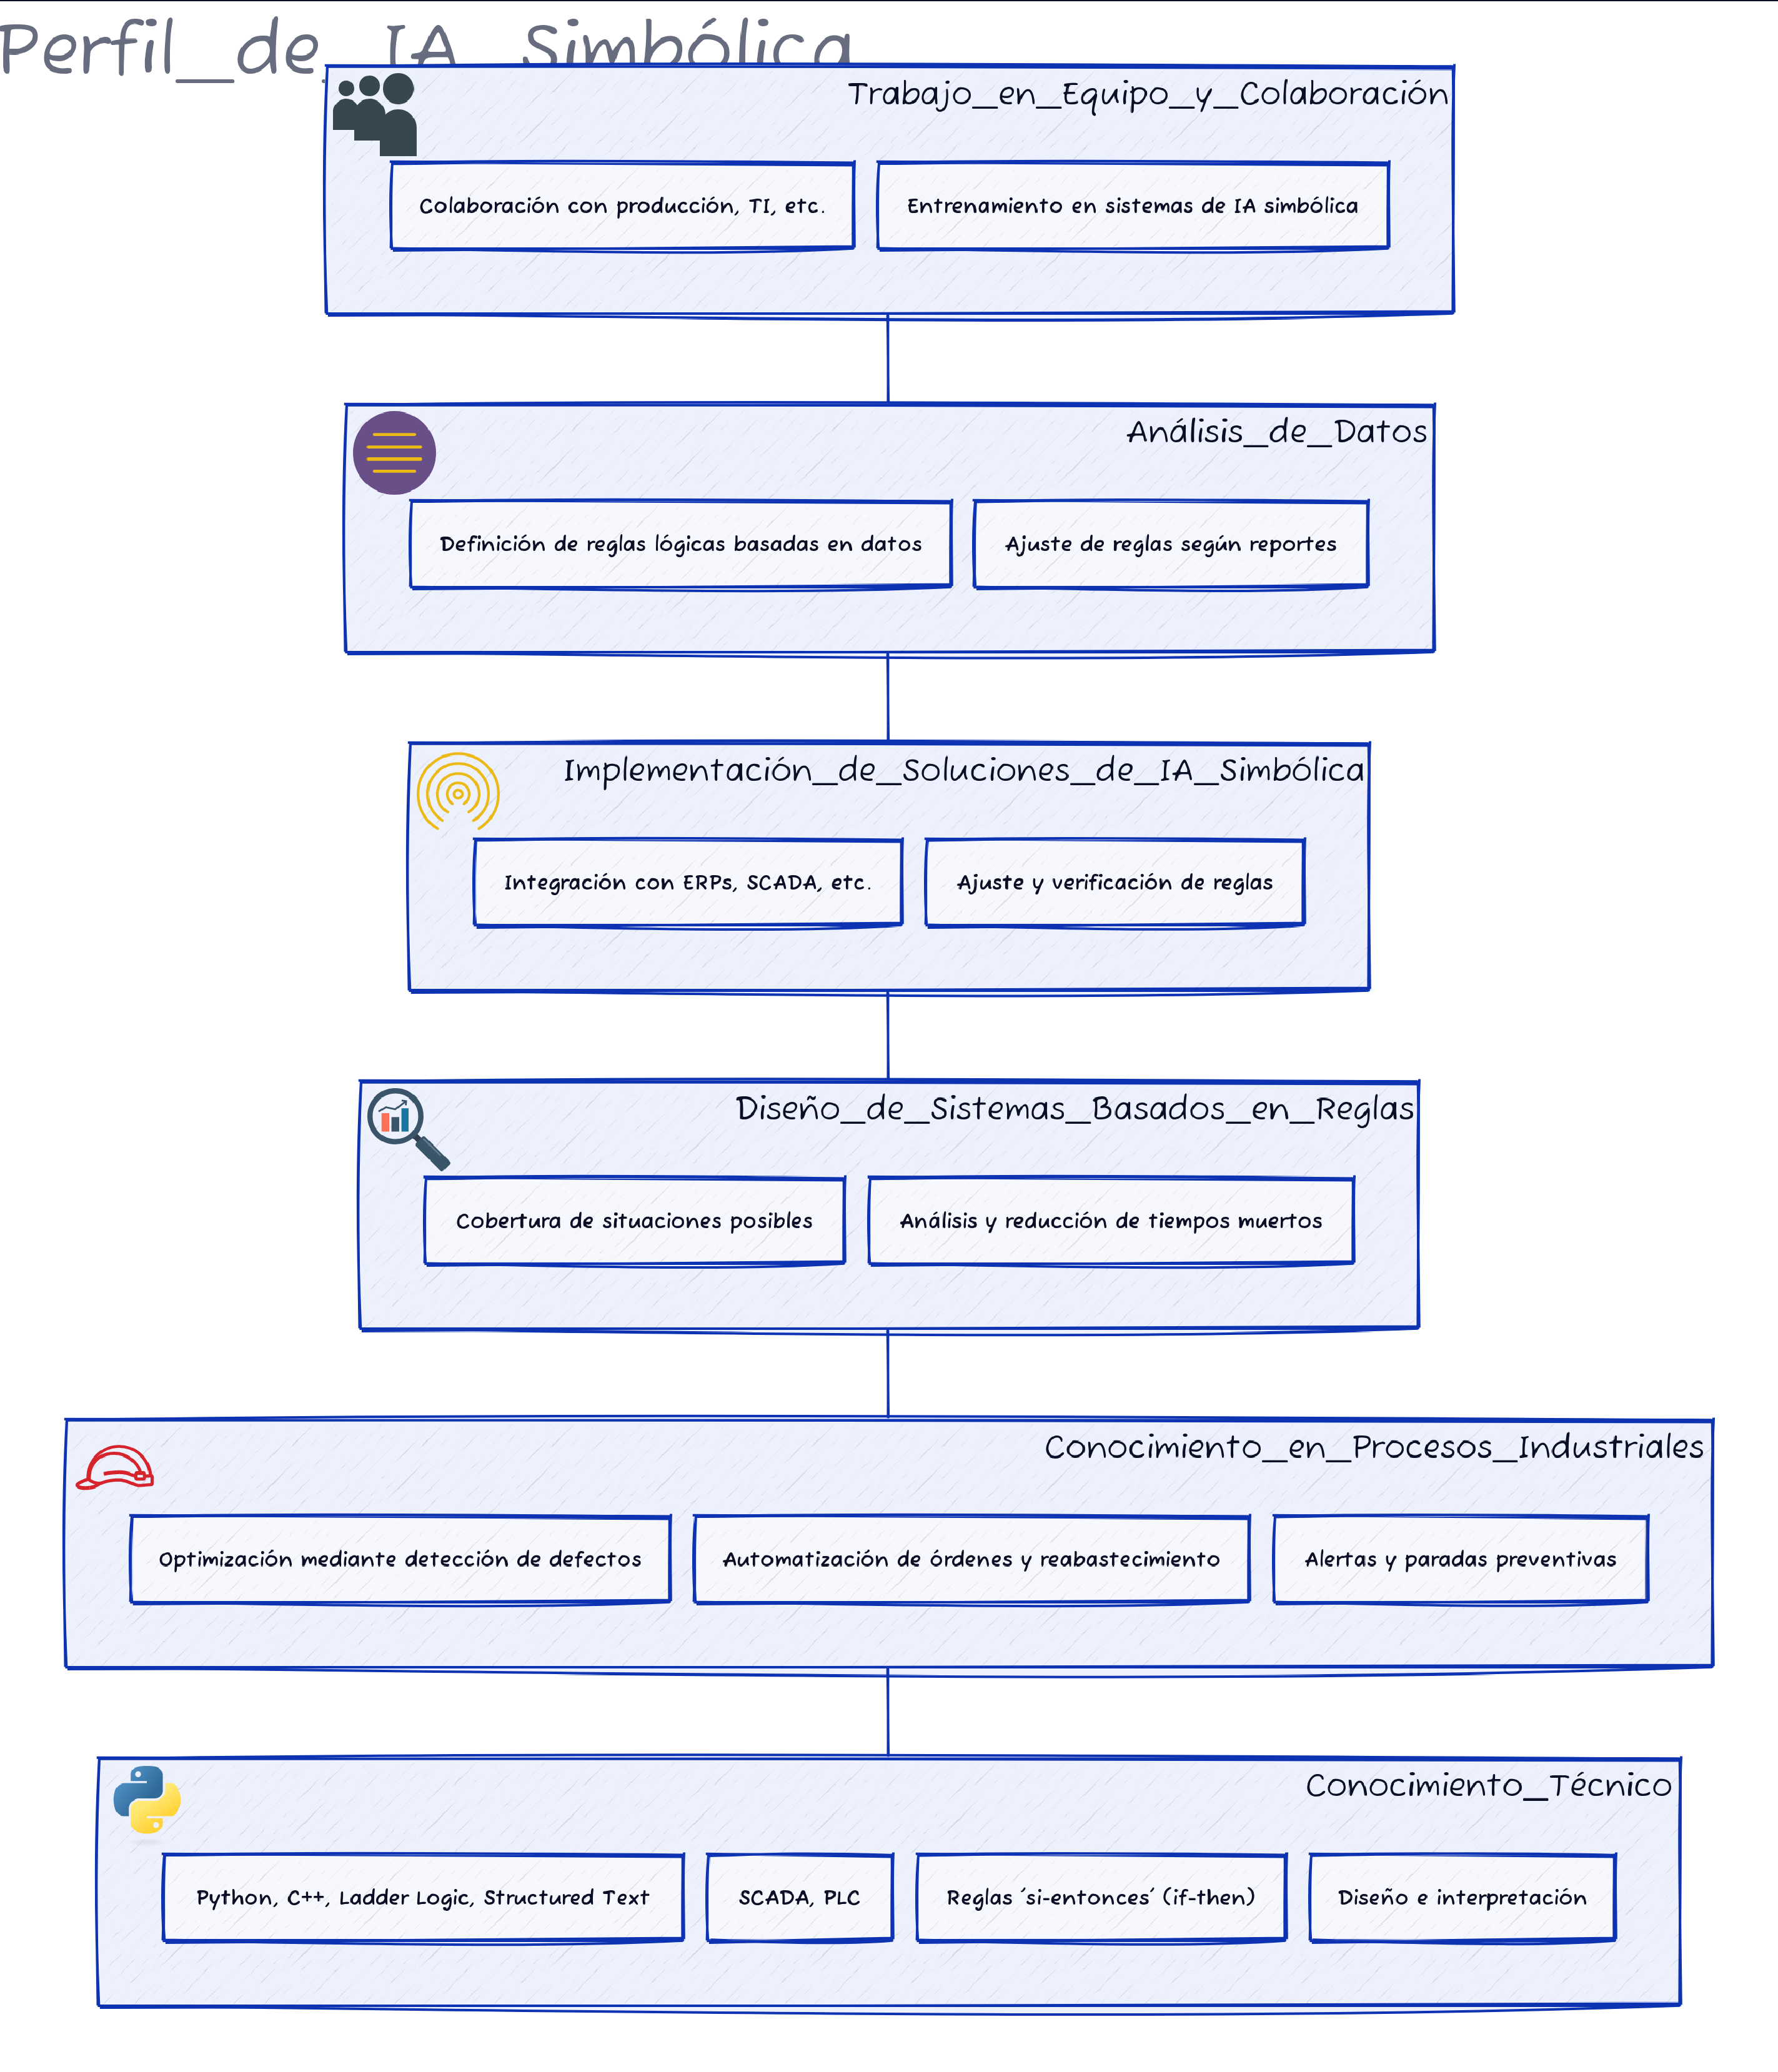
\includegraphics[width=1\textwidth,height=\textheight]{index_files/mediabag/diagram-3.pdf}

\subsection{\texorpdfstring{\textbf{Resumen del
Perfil}}{Resumen del Perfil}}\label{resumen-del-perfil}

\begin{enumerate}
\def\labelenumi{\arabic{enumi}.}
\tightlist
\item
  \textbf{Conocimiento Técnico}: Programación, lógica de sistemas, y
  diagramas de flujo.
\item
  \textbf{Entendimiento de Procesos Industriales}: Control de calidad,
  gestión de inventarios y mantenimiento preventivo.
\item
  \textbf{Diseño de Sistemas Basados en Reglas}: Desarrollo de reglas
  condicionales y flujos de decisión claros.
\item
  \textbf{Experiencia Práctica}: Implementación, configuración y ajuste
  de sistemas de IA simbólica en ambientes reales.
\item
  \textbf{Análisis de Datos}: Uso de datos históricos para definir
  reglas efectivas.
\item
  \textbf{Trabajo en Equipo}: Colaboración con distintos departamentos y
  capacidad de entrenamiento al personal.
\end{enumerate}

Este perfil es fundamental para garantizar que la maquiladora pueda
implementar con éxito un sistema de \textbf{IA simbólica} que automatice
tareas repetitivas, mejore la eficiencia y minimice los errores humanos,
todo con un enfoque basado en reglas claras y predefinidas. \#NOTA
AGREAGAR IA NOTA AUTOR

\#\#\# Conocimientos Previos para Machine Learning: Dataset y Tipos de
Variables

El \textbf{Machine Learning (ML)}, o aprendizaje automático, es una rama
de la inteligencia artificial que permite a las máquinas aprender de los
datos y hacer predicciones o tomar decisiones sin ser programadas de
forma explícita para cada tarea. Sin embargo, para comprender cómo
funciona y aprovechar al máximo el Machine Learning en la maquiladora,
primero es necesario entender algunos \textbf{conceptos clave}, como lo
son los \textbf{datasets} y los \textbf{tipos de variables}.

En este capítulo, exploraremos estos conceptos fundamentales que te
permitirán navegar y aplicar con éxito el Machine Learning en tus
procesos industriales.

\subsubsection{¿Qué es un Dataset?}\label{quuxe9-es-un-dataset}

Un \textbf{dataset} es simplemente un conjunto de datos que se utiliza
para entrenar y evaluar un modelo de Machine Learning. \textbf{Imagina}
que es como una hoja de cálculo de Excel, donde cada fila es una
instancia o un ejemplo de los datos, y cada columna es una
característica o variable que describe ese ejemplo.

\begin{itemize}
\tightlist
\item
  \textbf{Filas (Instancias)}: Cada fila representa un ejemplo o caso
  dentro del dataset. En el caso de una maquiladora, cada fila podría
  ser un producto individual, una máquina en operación, o una medición
  de calidad.
\item
  \textbf{Columnas (Características/Variables)}: Cada columna describe
  un aspecto o atributo del ejemplo. Esto podría incluir cosas como la
  temperatura de una máquina, el tiempo de operación, o el tamaño de un
  producto.
\end{itemize}

\textbf{Ejemplo en la Maquiladora}: - \textbf{Instancia (Fila)}: Un
producto ensamblado en la línea de producción. - \textbf{Variables
(Columnas)}: Peso del producto, dimensiones, número de piezas
defectuosas, tiempo de ensamblaje, etc.

\subsubsection{Tipos de Datasets}\label{tipos-de-datasets}

En Machine Learning, los datasets se suelen dividir en dos grandes
categorías:

\begin{enumerate}
\def\labelenumi{\arabic{enumi}.}
\item
  \textbf{Dataset de Entrenamiento}: Este es el conjunto de datos que se
  utiliza para entrenar al modelo de Machine Learning. El modelo aprende
  los patrones y relaciones de los datos en este conjunto.
\item
  \textbf{Dataset de Prueba (Test)}: Este conjunto de datos se utiliza
  para evaluar el rendimiento del modelo una vez que ha sido entrenado.
  Es un conjunto nuevo para el modelo, lo que permite medir su capacidad
  de hacer predicciones precisas en datos no vistos antes.
\end{enumerate}

\subsubsection{Tipos de Variables}\label{tipos-de-variables}

Al trabajar con Machine Learning, es crucial entender los tipos de
variables que forman parte de tu dataset. Estas variables o
características son las que el modelo va a utilizar para aprender y
hacer predicciones. Existen principalmente dos tipos de variables:
\textbf{variables numéricas} y \textbf{variables categóricas}.

\subsubsection{\texorpdfstring{1. \textbf{Variables
Numéricas}}{1. Variables Numéricas}}\label{variables-numuxe9ricas}

Las \textbf{variables numéricas} son aquellas que representan valores
cuantitativos. Es decir, aquellas que pueden ser medidas en forma de
números y en las que tiene sentido realizar operaciones matemáticas como
suma o promedio. Se dividen en dos tipos:

\begin{itemize}
\item
  \textbf{Variables Continuas}: Pueden tomar un rango infinito de
  valores. \textbf{Ejemplo}: La temperatura de una máquina (35.5°C,
  36.2°C, etc.) o el tiempo de producción de un producto (en horas o
  minutos).
\item
  \textbf{Variables Discretas}: Solo pueden tomar un conjunto limitado
  de valores específicos. \textbf{Ejemplo}: El número de productos
  defectuosos en una línea de producción (1, 2, 3, etc.).
\end{itemize}

\textbf{Ejemplo en la Maquiladora}: - \textbf{Variable Continua}: El
peso de una pieza fabricada. - \textbf{Variable Discreta}: El número de
paradas que tuvo una máquina en un día.

\paragraph{\texorpdfstring{2. \textbf{Variables
Categóricas}}{2. Variables Categóricas}}\label{variables-categuxf3ricas}

Las \textbf{variables categóricas} son aquellas que describen categorías
o grupos. No tienen un valor numérico, sino que clasifican los datos en
diferentes categorías. Se dividen en:

\begin{itemize}
\item
  \textbf{Nominales}: No tienen un orden específico entre las
  categorías. \textbf{Ejemplo}: Los colores de un producto (rojo, azul,
  verde) o los tipos de defectos (fisura, deformación, etc.).
\item
  \textbf{Ordinales}: Tienen un orden jerárquico entre las categorías.
  \textbf{Ejemplo}: La calificación de calidad del producto (alta,
  media, baja) o los niveles de urgencia para el mantenimiento de una
  máquina (alto, medio, bajo).
\end{itemize}

\textbf{Ejemplo en la Maquiladora}: - \textbf{Variable Nominal}: Tipo de
máquina (ensambladora, soldadora, cortadora). - \textbf{Variable
Ordinal}: Clasificación de prioridad para el mantenimiento de máquinas
(urgente, normal, bajo).

\subsubsection{¿Por Qué Es Importante Entender los Tipos de
Variables?}\label{por-quuxe9-es-importante-entender-los-tipos-de-variables}

Saber qué tipo de variable estás utilizando en tu dataset es crucial
porque influye en cómo se entrenará el modelo de Machine Learning.
Algunos modelos trabajan mejor con variables numéricas, mientras que
otros pueden manejar variables categóricas.

Por ejemplo: - Un modelo de regresión lineal solo puede trabajar con
\textbf{variables numéricas}. - Un árbol de decisión puede trabajar
tanto con \textbf{variables numéricas} como \textbf{categóricas}.

Además, algunos tipos de variables pueden requerir preprocesamiento
antes de ser usados por un modelo de Machine Learning. \textbf{Las
variables categóricas}, por ejemplo, a menudo deben ser codificadas
(convertidas en números) antes de ser procesadas por el modelo.

\subsubsection{Ejemplo en la Maquiladora: Dataset de Mantenimiento
Predictivo}\label{ejemplo-en-la-maquiladora-dataset-de-mantenimiento-predictivo}

Supongamos que deseas implementar un sistema de \textbf{mantenimiento
predictivo} en tu maquiladora, utilizando Machine Learning. Para ello,
necesitas crear un dataset que contenga variables relevantes sobre el
estado de tus máquinas. Este dataset podría verse así:

\begin{longtable}[]{@{}
  >{\raggedright\arraybackslash}p{(\columnwidth - 8\tabcolsep) * \real{0.1412}}
  >{\raggedright\arraybackslash}p{(\columnwidth - 8\tabcolsep) * \real{0.1529}}
  >{\raggedright\arraybackslash}p{(\columnwidth - 8\tabcolsep) * \real{0.2353}}
  >{\raggedright\arraybackslash}p{(\columnwidth - 8\tabcolsep) * \real{0.2000}}
  >{\raggedright\arraybackslash}p{(\columnwidth - 8\tabcolsep) * \real{0.2706}}@{}}
\toprule\noalign{}
\begin{minipage}[b]{\linewidth}\raggedright
ID Máquina
\end{minipage} & \begin{minipage}[b]{\linewidth}\raggedright
Temperatura
\end{minipage} & \begin{minipage}[b]{\linewidth}\raggedright
Horas de Operación
\end{minipage} & \begin{minipage}[b]{\linewidth}\raggedright
Tipo de Máquina
\end{minipage} & \begin{minipage}[b]{\linewidth}\raggedright
Mantenimiento Urgente
\end{minipage} \\
\midrule\noalign{}
\endhead
\bottomrule\noalign{}
\endlastfoot
1 & 85°C & 200 & Soldadora & Sí \\
2 & 70°C & 300 & Ensambladora & No \\
3 & 90°C & 180 & Cortadora & Sí \\
\end{longtable}

\textbf{Variables en el Dataset:} - \textbf{ID Máquina}: Variable
numérica (discreta), utilizada solo para identificar. -
\textbf{Temperatura}: Variable numérica (continua), describe la
temperatura actual de la máquina. - \textbf{Horas de Operación}:
Variable numérica (continua), describe cuántas horas ha estado en
funcionamiento la máquina. - \textbf{Tipo de Máquina}: Variable
categórica (nominal), describe el tipo de máquina. -
\textbf{Mantenimiento Urgente}: Variable categórica (ordinal), indica si
la máquina necesita o no mantenimiento.

Este dataset puede ser usado para entrenar un modelo de Machine Learning
que prediga si una máquina va a necesitar mantenimiento en el futuro. El
modelo analizaría las variables (temperatura, horas de operación, tipo
de máquina) para predecir cuándo será necesario el mantenimiento.

\subsubsection{Conclusión}\label{conclusiuxf3n}

Entender los conceptos de \textbf{dataset} y \textbf{tipos de variables}
es fundamental para comenzar a trabajar con \textbf{Machine Learning} en
la maquiladora. Estos conocimientos previos te permitirán preparar tus
datos de manera adecuada, elegir el tipo de modelo más adecuado y lograr
que tu sistema de aprendizaje automático funcione de manera eficiente.

Al manejar correctamente las \textbf{variables numéricas} y
\textbf{categóricas}, y al estructurar bien tu \textbf{dataset}, estarás
dando un paso importante hacia la implementación efectiva de Machine
Learning en tus procesos, ya sea para predecir fallos en las máquinas,
optimizar la calidad del producto o gestionar eficientemente los
inventarios.

Aquí tienes las dos primeras partes del capítulo con más texto y una
explicación menos técnica, adaptada para una mejor comprensión y sin
perder el enfoque en la maquiladora:

\section{Aplicaciones de Machine Learning en la
Maquiladora}\label{aplicaciones-de-machine-learning-en-la-maquiladora}

\subsection{\texorpdfstring{\textbf{Introducción a Machine Learning
(ML)}}{Introducción a Machine Learning (ML)}}\label{introducciuxf3n-a-machine-learning-ml}

El \textbf{Machine Learning} es una herramienta clave en el avance
tecnológico de las maquiladoras. Aunque suena como un concepto
complicado, en realidad es más sencillo de lo que parece: se trata de
enseñar a las máquinas a \textbf{aprender} de los datos, tal como
nosotros aprendemos de la experiencia. En lugar de programar una máquina
para que haga exactamente lo que queremos (como en los sistemas
tradicionales), \textbf{Machine Learning (ML)} permite que las máquinas
identifiquen patrones, hagan predicciones y tomen decisiones basadas en
esos datos.

Entonces, \textbf{¿por qué esto es importante para una maquiladora?}
Porque la IA y el Machine Learning pueden ayudar a reducir errores,
optimizar la producción, mejorar la calidad y anticipar problemas antes
de que ocurran. Si tu línea de producción tiene un historial de fallas
que cuesta tiempo y dinero, ¿no sería genial que una máquina te avisara
antes de que suceda para que pudieras arreglarlo de antemano?

\begin{figure}[H]

{\centering 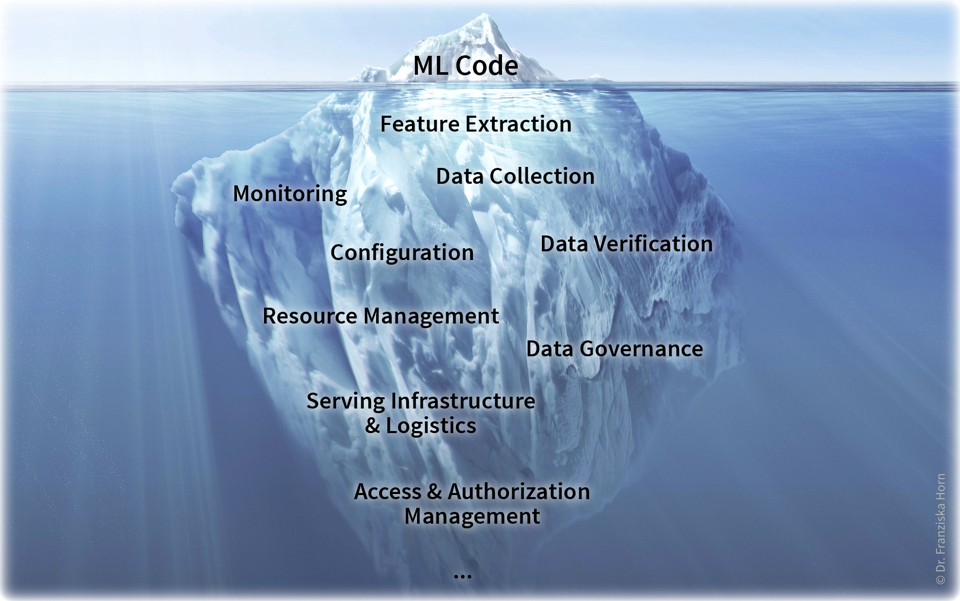
\includegraphics{Img/imagen_186.jpg}

}

\caption{Iceber}

\end{figure}%

\subsubsection{\texorpdfstring{\textbf{¿Qué es Machine
Learning?}}{¿Qué es Machine Learning?}}\label{quuxe9-es-machine-learning}

El \textbf{Machine Learning} se basa en la idea de que una máquina puede
aprender a hacer algo (como predecir fallas o mejorar un proceso)
simplemente dándole acceso a muchos datos sobre ese algo. \textbf{Es
como enseñar a alguien a resolver un problema dándole ejemplos de cómo
se ha resuelto ese problema antes.}

Imagina que tienes datos sobre la producción de una máquina: las horas
que opera, las temperaturas que alcanza, la cantidad de piezas que
fabrica, etc. Si cada vez que la máquina fallaba también anotabas estas
mismas características, podrías darle esos datos a un modelo de Machine
Learning, y este aprendería a identificar las condiciones que llevan a
una falla. \textbf{Básicamente, se trata de darle a la máquina un
``historial'' de lo que ha pasado, para que pueda predecir lo que pasará
en el futuro}.

En resumen: \textbf{Machine Learning} es el arte de hacer que las
máquinas aprendan de los datos, para que puedan tomar decisiones o hacer
predicciones sin que les digas exactamente qué hacer en cada caso.
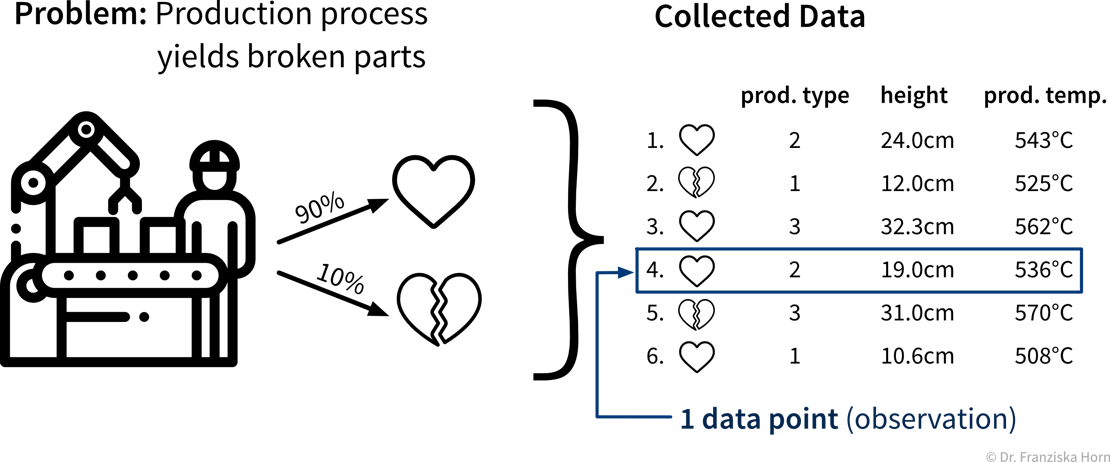
\includegraphics{Img/imagen_32.jpg}

\subsubsection{\texorpdfstring{\textbf{Aprendizaje Supervisado vs No
Supervisado}}{Aprendizaje Supervisado vs No Supervisado}}\label{aprendizaje-supervisado-vs-no-supervisado}

Existen dos tipos principales de Machine Learning, y entender la
diferencia entre ellos te ayudará a identificar cuál es más útil en tu
maquila.

\subsubsection{\texorpdfstring{\textbf{Aprendizaje
Supervisado}}{Aprendizaje Supervisado}}\label{aprendizaje-supervisado}

El \textbf{aprendizaje supervisado} es como enseñarle a alguien a hacer
algo mostrándole los ejemplos correctos y las respuestas. Le das a la
máquina un conjunto de datos donde ya sabes lo que pasa (el resultado),
y la máquina aprende a predecir ese resultado cuando vea datos nuevos.

\textbf{Ejemplo sencillo en la maquila}: Supón que tienes los datos de
las máquinas en tu línea de producción y sabes qué condiciones llevaron
a una falla (como vibraciones anormales o temperaturas extremas). Puedes
entrenar a un modelo de Machine Learning para que, cuando vea esas
mismas condiciones en una máquina en funcionamiento, te avise de que
algo está mal antes de que ocurra una avería.

Este tipo de ML funciona muy bien cuando ya tienes información sobre lo
que ha ocurrido y quieres predecir lo que sucederá en situaciones
similares en el futuro.

\subsubsection{\texorpdfstring{\textbf{Aprendizaje No
Supervisado}}{Aprendizaje No Supervisado}}\label{aprendizaje-no-supervisado}

Por otro lado, el \textbf{aprendizaje no supervisado} es un poco más
libre: es como darle un montón de información a la máquina y dejarla que
descubra patrones por sí sola. No le dices qué debe buscar, simplemente
la máquina agrupa los datos o encuentra similitudes entre ellos.

\textbf{Ejemplo sencillo en la maquila}: Digamos que tienes muchos datos
sobre el rendimiento de tus máquinas, pero no sabes qué está afectando a
la producción. Con el aprendizaje no supervisado, puedes descubrir
patrones en los datos, como que ciertas máquinas siempre rinden menos a
ciertas horas del día o cuando operan junto a otras máquinas
específicas. La IA encontrará esos patrones, lo que te permitirá hacer
ajustes en la producción que de otro modo no habrías notado.

\subsubsection{El papel de ML en la maquila: ¿Por qué es
importante?**}\label{el-papel-de-ml-en-la-maquila-por-quuxe9-es-importante}

Machine Learning puede transformar radicalmente la manera en que operas
en la maquiladora. \textbf{¿Por qué?} Porque la IA no solo se trata de
automatizar, sino de hacer más inteligentes las decisiones que tomas día
a día.

\textbf{Imagina esto}: Tienes una línea de producción donde algunas
máquinas fallan de vez en cuando. Esto significa paradas inesperadas,
retrasos, y por supuesto, costos adicionales. Pero ¿qué pasaría si
pudieras predecir cuándo esas máquinas van a fallar y hacer el
mantenimiento antes de que ocurra la avería? Esto es lo que Machine
Learning puede hacer por ti. Es como tener un ``sexto sentido'' en la
producción.

Además, no solo hablamos de evitar fallas: Machine Learning puede
ayudarte a ajustar el inventario de manera eficiente, prever la demanda,
mejorar la calidad de los productos, y hasta optimizar la logística
dentro de la planta. En resumen, \textbf{es una herramienta para ser más
competitivo en un mercado que no para de moverse}.

\subsection{\texorpdfstring{\textbf{Tipos de Machine Learning en la
Maquila}}{Tipos de Machine Learning en la Maquila}}\label{tipos-de-machine-learning-en-la-maquila}

Ahora que ya tienes una idea básica de lo que es Machine Learning y por
qué es tan relevante en la maquiladora, vamos a profundizar un poco más
en los tipos de ML que puedes utilizar en tu planta. Dependiendo del
tipo de problema que enfrentes, puedes elegir entre \textbf{aprendizaje
supervisado} o \textbf{no supervisado}, e incluso otros enfoques como el
\textbf{aprendizaje por refuerzo}.

\begin{figure}[H]

{\centering 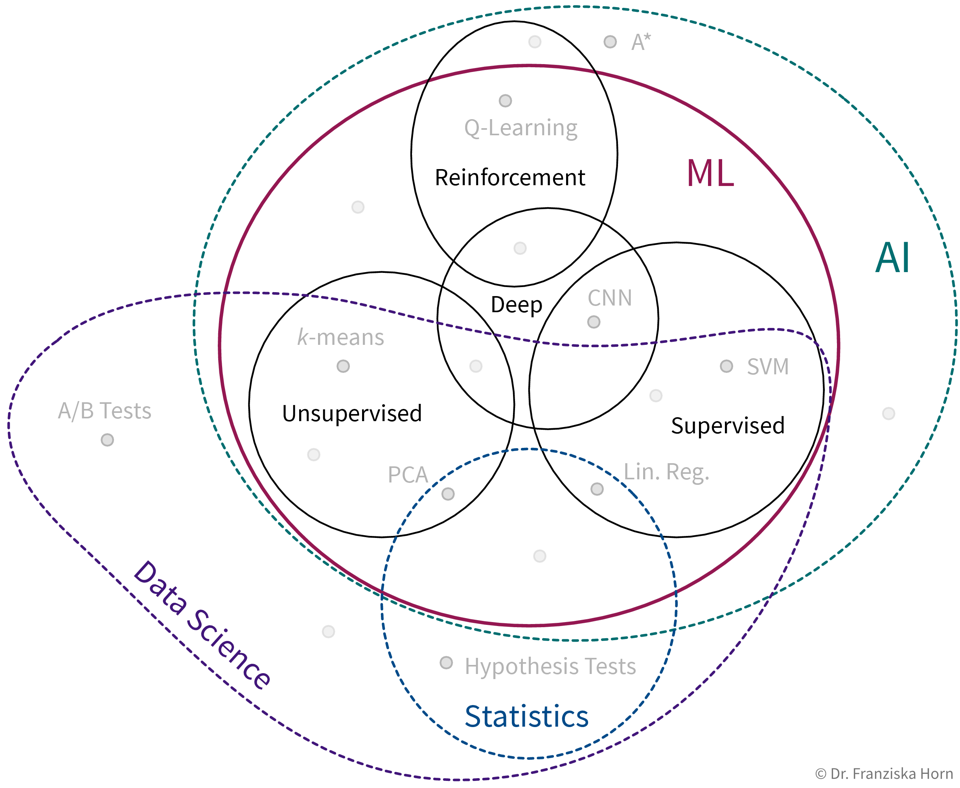
\includegraphics{Img/imagen_21.jpg}

}

\caption{Tipos}

\end{figure}%

\subsubsection{\texorpdfstring{\textbf{Aprendizaje
Supervisado}}{Aprendizaje Supervisado}}\label{aprendizaje-supervisado-1}

En el \textbf{aprendizaje supervisado}, el sistema aprende de datos que
ya incluyen tanto las características (por ejemplo, temperatura de la
máquina, tiempo de operación, etc.) como los resultados correctos (por
ejemplo, si la máquina falló o no). Este tipo de aprendizaje es ideal
cuando ya tienes un montón de información de tus procesos y quieres
usarla para predecir futuros eventos.

\textbf{Ejemplo práctico}: Si sabes que ciertas condiciones en una
máquina han llevado a su falla en el pasado, puedes entrenar un modelo
de aprendizaje supervisado que prediga cuándo una máquina fallará de
nuevo basándose en esas mismas condiciones. Esto es útil para el
\textbf{mantenimiento predictivo}, que puede ahorrarte mucho tiempo y
dinero.

Con aprendizaje supervisado, el sistema va afinando su capacidad de
predecir o clasificar con base en los patrones que ha encontrado en los
datos pasados. Es como si entrenaras a alguien nuevo en tu maquila
mostrándole qué debe hacer y qué no debe hacer con ejemplos concretos.

\subsubsection{\texorpdfstring{\textbf{Aprendizaje No
Supervisado}}{Aprendizaje No Supervisado}}\label{aprendizaje-no-supervisado-1}

El \textbf{aprendizaje no supervisado} es como darle a la máquina una
pila de datos y decirle ``¡descubre algo interesante!''. No le damos las
respuestas de antemano, sino que la máquina encuentra patrones por su
cuenta.

\textbf{Ejemplo práctico}: Puedes usar aprendizaje no supervisado para
analizar datos de producción y descubrir relaciones que no habías visto
antes. Por ejemplo, podrías descubrir que ciertas combinaciones de
máquinas tienden a producir más errores en ciertos momentos del día.
Este tipo de información es oro puro para optimizar la producción, ya
que te permite tomar decisiones informadas basadas en lo que los datos
te dicen, no en suposiciones.

Este enfoque es útil cuando no sabes exactamente qué buscar en tus
datos, pero sospechas que hay información valiosa escondida en ellos. La
máquina encuentra esas conexiones por ti. Gracias por tus comentarios. A
continuación, te dejo el mismo flujo que has aprobado, pero con más
texto para enriquecer los capítulos y dar mayor contexto a cada sección.

\subsection{Conceptos Clave para Entender Machine
Learning}\label{conceptos-clave-para-entender-machine-learning}

Para implementar \textbf{Machine Learning (ML)} de manera efectiva en
una maquiladora, es fundamental comprender algunos conceptos clave que
forman la base del aprendizaje automático. Estos términos te ayudarán a
abordar los desafíos técnicos y a tomar decisiones más inteligentes a
medida que avances en tu proceso de transformación digital.

\subsubsection{\texorpdfstring{\textbf{Dataset: La Base de
Todo}}{Dataset: La Base de Todo}}\label{dataset-la-base-de-todo}

Un \textbf{dataset} es el conjunto de datos que alimenta al modelo de
Machine Learning. \textbf{Piensa en el dataset como si fuera la materia
prima de una maquiladora}, donde los datos son las piezas que la IA
utiliza para aprender. Sin un buen dataset, el modelo no puede funcionar
correctamente.

\textbf{Ejemplo en la maquila}: Supongamos que tienes datos históricos
sobre las temperaturas de las máquinas, el tiempo que han estado
operativas, el número de piezas que han producido y cuándo fallaron. Ese
conjunto de datos es el ``dataset'' que alimentará tu modelo para que
pueda aprender a predecir cuándo fallará una máquina en el futuro.

Es importante tener en cuenta que la calidad de los datos es
fundamental. Si los datos son incorrectos o incompletos, el modelo
aprenderá mal. Es lo que decimos en Machine Learning: \textbf{``Garbage
in, garbage out''}. Si le das basura al modelo, los resultados también
serán basura.

\subsubsection{\texorpdfstring{\textbf{Variables Dependientes e
Independientes}}{Variables Dependientes e Independientes}}\label{variables-dependientes-e-independientes}

En Machine Learning, las \textbf{variables} son los elementos de los
datos que influyen en los resultados. Hay dos tipos de variables que
debes conocer:

\begin{figure}[H]

{\centering 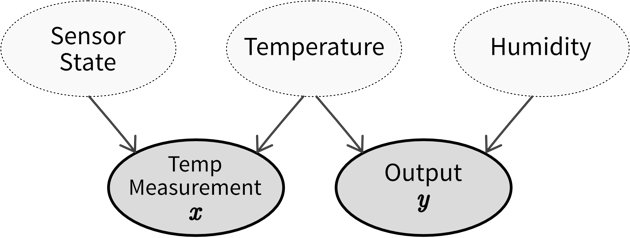
\includegraphics{Img/imagen_157.jpg}

}

\caption{Iceb}

\end{figure}%

\begin{itemize}
\item
  \textbf{Variables Independientes}: Son las entradas que proporcionan
  la información al modelo. Son como las características que describen
  un producto en una maquiladora. Por ejemplo, la temperatura de una
  máquina, la velocidad de producción o el número de horas trabajadas.
\item
  \textbf{Variable Dependiente}: Es la salida o el resultado que estamos
  intentando predecir. Es lo que queremos que la máquina aprenda a
  identificar o calcular. En una maquiladora, la variable dependiente
  podría ser si una máquina va a fallar o no, o la cantidad de piezas
  defectuosas que produce una línea de producción.
\end{itemize}

\textbf{Ejemplo práctico en producción}: Si estás tratando de predecir
fallos en tus máquinas, las variables independientes podrían ser la
vibración de las máquinas, la temperatura y las horas de operación. La
variable dependiente sería si la máquina falla o no.

El éxito de un modelo de Machine Learning depende de cuán bien
seleccionemos estas variables. Un buen conjunto de variables
independientes puede mejorar dramáticamente el rendimiento del modelo.

\subsubsection{\texorpdfstring{\textbf{Feature Engineering: La Clave del
Éxito}}{Feature Engineering: La Clave del Éxito}}\label{feature-engineering-la-clave-del-uxe9xito}

El \textbf{feature engineering} es el proceso de elegir, transformar y
crear las características (variables) que mejoran el rendimiento de un
modelo de Machine Learning. Este paso es esencial porque no todas las
variables son igual de útiles. Algunas variables pueden ser
irrelevantes, mientras que otras pueden tener un impacto significativo
en los resultados.

\textbf{Ejemplo en la maquila}: Si estás entrenando un modelo para
predecir cuándo fallará una máquina, probablemente no tenga sentido
incluir la \textbf{marca de la máquina} como una variable independiente.
Sin embargo, la \textbf{temperatura de operación} o la \textbf{cantidad
de horas trabajadas} probablemente sean factores mucho más importantes
que debes incluir.

El \textbf{feature engineering} te ayuda a seleccionar las variables
clave y a descartarlas irrelevantes. También puedes crear nuevas
variables a partir de las existentes. Por ejemplo, si tienes el dato de
la \textbf{temperatura} y el \textbf{número de horas trabajadas},
podrías crear una nueva variable que sea la \textbf{combinación de ambos
factores}, lo que podría mejorar las predicciones.

\subsubsection{\texorpdfstring{\textbf{Preprocesamiento de Datos:
Limpiando los
Datos}}{Preprocesamiento de Datos: Limpiando los Datos}}\label{preprocesamiento-de-datos-limpiando-los-datos}

El \textbf{preprocesamiento de datos} es uno de los pasos más
importantes para que un modelo de Machine Learning funcione
correctamente. \textbf{Imagina que tienes un coche muy potente, pero las
llantas están desinfladas. No importa qué tan bueno sea el motor, el
coche no va a funcionar bien.} Lo mismo pasa con los datos: si no están
limpios y organizados, tu modelo no rendirá como debería.

El preprocesamiento implica varias tareas, como: - \textbf{Limpieza de
Datos}: A veces, los datos están incompletos o tienen errores. Por
ejemplo, una máquina podría haber dejado de registrar datos durante
ciertos periodos de tiempo. En este caso, podrías necesitar eliminar
esos datos incompletos o estimar los valores que faltan.

\begin{itemize}
\tightlist
\item
  \textbf{Normalización}: Si tus variables tienen diferentes escalas,
  puede ser útil normalizarlas para que el modelo las procese
  correctamente. Por ejemplo, si una variable mide \textbf{horas de
  operación} (que puede ser un número muy grande) y otra mide
  \textbf{temperatura} (que es un número más pequeño), puedes escalarlas
  para que el modelo las trate de manera equilibrada.
\end{itemize}

El preprocesamiento es clave porque \textbf{los datos crudos no siempre
son útiles}. Limpiarlos y prepararlos adecuadamente te permite sacar el
máximo provecho de tu modelo de Machine Learning.

\begin{figure}[H]

{\centering 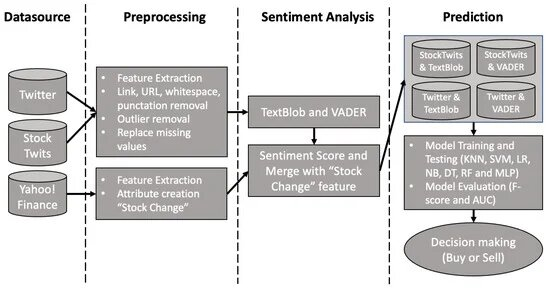
\includegraphics{Img/datasource.jpg}

}

\caption{Dataflow}

\end{figure}%

\subsection{Ventajas del Machine Learning en la
Maquiladora}\label{ventajas-del-machine-learning-en-la-maquiladora}

El \textbf{Machine Learning} ofrece muchas ventajas para una
maquiladora, desde la reducción de costos hasta la mejora en la
eficiencia de los procesos. Aquí te detallamos las principales razones
por las que integrar ML en tu maquila puede marcar la diferencia:

\subsubsection{\texorpdfstring{\textbf{Rapidez en la Toma de
Decisiones}}{Rapidez en la Toma de Decisiones}}\label{rapidez-en-la-toma-de-decisiones}

Una de las mayores ventajas del Machine Learning es la
\textbf{velocidad} con la que puede analizar grandes cantidades de datos
y ofrecer resultados. Esto es especialmente útil en una maquiladora,
donde la rapidez en la toma de decisiones puede marcar la diferencia
entre cumplir con un pedido o retrasarse.

\textbf{Ejemplo en la maquila}: Un modelo de ML puede analizar los datos
de rendimiento de las máquinas en tiempo real y enviar alertas
instantáneas cuando detecte que algo no está bien. Esto te permite
actuar de inmediato, evitando que pequeños problemas se conviertan en
grandes fallos.

\subsubsection{\texorpdfstring{\textbf{Facilidad de Uso y
Sencillez}}{Facilidad de Uso y Sencillez}}\label{facilidad-de-uso-y-sencillez}

Hoy en día, las herramientas de Machine Learning son cada vez más
accesibles, y muchas de ellas ofrecen interfaces simples que no
requieren conocimientos avanzados en programación. Incluso si tu equipo
no tiene experiencia con IA, \textbf{plataformas como AWS, Azure y
Google Cloud} te permiten implementar modelos de manera sencilla y
escalable.

\subsubsection{\texorpdfstring{\textbf{Auditoría y
Transparencia}}{Auditoría y Transparencia}}\label{auditoruxeda-y-transparencia}

Otra ventaja clave es que \textbf{los modelos de Machine Learning pueden
ser auditados}. Esto significa que puedes rastrear y verificar cómo el
modelo llegó a una decisión o predicción, lo que es muy importante en
industrias reguladas como la manufactura. Además, te permite ajustar los
modelos con base en los resultados que obtienes.

\textbf{Ejemplo en la maquila}: Si tu modelo predice que una máquina va
a fallar, puedes revisar los datos en los que basó esa predicción (como
la temperatura o la vibración) y ajustar las condiciones si crees que el
modelo está siendo demasiado sensible o no lo suficiente.

\subsection{Desventajas del Machine Learning en la
Maquiladora}\label{desventajas-del-machine-learning-en-la-maquiladora}

Aunque \textbf{Machine Learning} tiene muchas ventajas, no es una
solución mágica. Implementarlo también tiene desafíos y posibles
desventajas que debes tener en cuenta.

\subsubsection{\texorpdfstring{\textbf{Costo de
Implementación}}{Costo de Implementación}}\label{costo-de-implementaciuxf3n}

A pesar de las ventajas a largo plazo, el costo inicial de implementar
ML puede ser alto, especialmente si tu maquiladora no tiene ya la
infraestructura necesaria. \textbf{La compra de software, hardware
especializado y la contratación de talento} para administrar los
sistemas de Machine Learning pueden representar una barrera.

\textbf{Ejemplo}: Algunas maquiladoras pequeñas podrían no tener acceso
a los recursos necesarios para implementar ML de manera inmediata, por
lo que un enfoque escalonado o la externalización de servicios puede ser
una opción.

\subsubsection{\texorpdfstring{\textbf{Dudas
Técnicas}}{Dudas Técnicas}}\label{dudas-tuxe9cnicas}

El éxito de un sistema de Machine Learning depende mucho de la calidad
de los datos y del personal capacitado que pueda supervisar y ajustar
los modelos. Si no tienes un equipo con experiencia en \textbf{análisis
de datos} y \textbf{programación}, podrías enfrentar dificultades para
configurar y mantener el sistema.

\subsubsection{\texorpdfstring{\textbf{Complejidad en el Análisis de
Datos}}{Complejidad en el Análisis de Datos}}\label{complejidad-en-el-anuxe1lisis-de-datos}

El análisis de datos en Machine Learning no es una tarea sencilla.
Requiere tiempo y experiencia para preparar correctamente los datos,
seleccionar las variables adecuadas y ajustar los modelos. Además, los
datos en bruto que provienen de las máquinas a menudo tienen errores o
inconsistencias que deben resolverse antes de alimentar al modelo.

\subsection{Conclusión de las Ventajas y
Desventajas}\label{conclusiuxf3n-de-las-ventajas-y-desventajas}

En resumen, el \textbf{Machine Learning} tiene el potencial de
revolucionar la maquiladora, optimizando procesos, reduciendo costos y
mejorando la calidad de los productos

. Sin embargo, la implementación tiene desafíos que deben considerarse
cuidadosamente. Con una buena planificación, inversión y el equipo
adecuado, \textbf{ML puede transformar la operación de tu maquila y
mantenerte competitivo en un mercado global}.

\subsection{Referencias ML}\label{referencias-ml}

\begin{enumerate}
\def\labelenumi{\arabic{enumi}.}
\item
  Russell, S. \& Norvig, P. \emph{Artificial Intelligence: A Modern
  Approach} (4th ed.). Prentice Hall, 2020.
\item
  Goodfellow, I., Bengio, Y. \& Courville, A. \emph{Deep Learning}. MIT
  Press, 2016.
\item
  Hastie, T., Tibshirani, R. \& Friedman, J. \emph{The Elements of
  Statistical Learning: Data Mining, Inference, and Prediction} (2nd
  ed.). Springer, 2009.
\item
  Géron, A. \emph{Hands-On Machine Learning with Scikit-Learn, Keras,
  and TensorFlow} (2nd ed.). O'Reilly Media, 2019.
\item
  Murphy, K. P. \emph{Machine Learning: A Probabilistic Perspective}.
  MIT Press, 2012.
\item
  Bishop, C. M. \emph{Pattern Recognition and Machine Learning}.
  Springer, 2006.
\item
  Domingos, P. \emph{The Master Algorithm: How the Quest for the
  Ultimate Learning Machine Will Remake Our World}. Basic Books, 2015.
\item
  Martínez, Oscar. \emph{Ciudad Juárez: El auge de una ciudad fronteriza
  a partir de 1848}. FCE, México, 1982.
\item
  Dirección General de Estadística, S.I.C. \emph{La Frontera Norte,
  Diagnóstico y Perspectivas}. Mimeo.
\item
  Madison, Thomas. \emph{Reseña Anual de la Industria Maquiladora}.
  SUGUMEX, México, 1990.
\item
  Bass Zavala, Sonia. ``El crecimiento urbano en Ciudad Juárez,
  1950-2000. Un acercamiento socio-histórico a la evolución desordenada
  de una ciudad de la frontera norte.'' \emph{Chihuahua Hoy} (2013):
  247-289.
\item
  Diario de Juárez, 21 a 24 de agosto de 1981.
\item
  El Fronterizo, 25 de agosto de 1974.
\item
  Ramos, Guadalupe. \emph{Norte}, 9 de febrero de 1994, p.~4A.
\item
  Diario de Juárez, 22 de mayo de 1991.
\item
  Diario de Juárez, 7 de febrero de 1991.
\item
  Luna, José Manuel. Declaración en \emph{Novedades}, 20 de enero de
  1985.
\item
  Vega, Luis. ``La transformación de la industria maquiladora en la era
  digital.'' \emph{El Financiero}, 2023.
\item
  Secretaría de Economía. ``Informe Anual sobre la Industria
  Maquiladora''. Gobierno de México, 2022. \#\#\# Conceptos para
  entender el siguiente capítulo
\end{enumerate}

\subsection{¿Qué es la NLP?}\label{quuxe9-es-la-nlp}

El procesamiento de lenguaje natural (NLP) es una tecnología de machine
learning que brinda a las computadoras la capacidad de interpretar,
manipular y comprender el lenguaje humano.

\subsection{API}\label{api}

Una API, o Interfaz de Programación de Aplicaciones, es un conjunto de
reglas y especificaciones que facilitan la comunicación e intercambio de
datos entre distintas aplicaciones de software. Actúan como puentes
digitales, permitiendo que software desarrollado con diferentes
tecnologías interactúe de forma fluida y segura.

La adopción de APIs es crucial en el panorama tecnológico actual, ya que
ofrece múltiples ventajas:

\begin{itemize}
\tightlist
\item
  \textbf{Reducción de costos y complejidad:} En lugar de desarrollar
  todas las funcionalidades desde cero, las empresas pueden integrar
  servicios externos a través de APIs, ahorrando tiempo, dinero y
  recursos en infraestructura y mantenimiento.
\item
  \textbf{Impulso a la innovación:} Las APIs permiten a los
  desarrolladores crear nuevas aplicaciones y servicios de forma más
  ágil, aprovechando funcionalidades ya existentes. Esto fomenta la
  creatividad y acelera la llegada de nuevas soluciones al mercado.
\item
  \textbf{Experiencias de usuario mejoradas:} La integración de
  múltiples aplicaciones a través de APIs permite ofrecer experiencias
  más completas y personalizadas.
\end{itemize}

\textbf{Ejemplos}

Imaginemos que estás desarrollando una aplicación financiera. En lugar
de construir desde cero un sistema complejo para manejar transacciones
de criptomonedas, puedes utilizar la API. Esta API te permitirá acceder
a funcionalidades como:

\begin{itemize}
\tightlist
\item
  Consultar precios de criptomonedas en tiempo real
\item
  Ejecutar órdenes de compra y venta
\item
  Resumen de un PDF./\ldots\ldots\ldots.
\item
  Chatear con asistente
\end{itemize}

De esta forma, te enfocas en desarrollar las características únicas de
tu aplicación, mientras aprovechas la infraestructura robusta y segura
de Gemini para gestionar las operaciones con criptomonedas. ¡Claro!
Vamos a explorar más términos clave relacionados con ChatGPT para que
tengas una comprensión más completa:

\textbf{1. Modelos de Lenguaje Largo (LLM)}

\begin{itemize}
\tightlist
\item
  \textbf{¿Qué son?} Son programas de computadora muy sofisticados que
  han ``leído'' una cantidad enorme de texto en internet. Esto les
  permite aprender patrones, gramática e incluso un poco de sentido
  común.
\item
  \textbf{¿Cómo funcionan?} Usan redes neuronales complejas para
  procesar el lenguaje, lo que les permite generar texto, traducir
  idiomas, responder preguntas e incluso escribir código.
\item
  \textbf{Ejemplo:} ChatGPT es un ejemplo de LLM. Su ``cerebro'' es un
  modelo de lenguaje largo que le permite entender y responder a tus
  preguntas de manera coherente.
\end{itemize}

\textbf{2. Tokens}

\begin{itemize}
\tightlist
\item
  \textbf{¿Qué son?} Son las unidades básicas en las que se divide el
  texto para que el modelo de lenguaje lo procese. Pueden ser palabras
  completas, partes de palabras o incluso signos de puntuación.
\item
  \textbf{¿Por qué son importantes?} Los modelos de lenguaje trabajan
  con tokens, no con letras individuales. Esto les permite entender el
  contexto y las relaciones entre las palabras.
\item
  \textbf{Ejemplo:} La frase ``Hola, ¿cómo estás?'' se divide en 5
  tokens: ``Hola'', ``,'', ``¿cómo'', ``estás'' y ``?''.
\end{itemize}

\textbf{3. Prompt}

\begin{itemize}
\tightlist
\item
  \textbf{¿Qué es?} Es el texto que le das a ChatGPT para iniciar una
  conversación o pedirle que haga algo. Puede ser una pregunta, una
  instrucción o incluso el comienzo de una historia.
\item
  \textbf{¿Por qué es importante?} El prompt le da a ChatGPT el contexto
  y la dirección para generar una respuesta relevante y útil.
\item
  \textbf{Ejemplo:} ``Escribe un poema sobre la primavera'' es un prompt
  que le indica a ChatGPT qué tipo de respuesta generar.
\end{itemize}

\section{La nueva era IA generativa}\label{la-nueva-era-ia-generativa}

\subsection{Introducción a la Inteligencia Artificial en la
Maquiladora}\label{introducciuxf3n-a-la-inteligencia-artificial-en-la-maquiladora}

Sabemos que el primer acercamiento que muchas personas tienen con la
\textbf{inteligencia artificial (IA)} hoy en día es a través de
herramientas como \textbf{ChatGPT} o servicios similares que utilizan
procesamiento de lenguaje natural (\emph{Natural Language Processing,
NLP}). Estos sistemas permiten a la IA entender y comunicarse en el
lenguaje humano, como el español o el inglés, sin necesidad de
interfaces complejas o técnicas.

\textbf{ChatGPT} fue una de las primeras plataformas en acercar la IA al
usuario común. Pero, ¿qué hace que esta tecnología sea tan especial? En
esencia, \textbf{ChatGPT} y otros sistemas similares se basan en
\textbf{NLP}, lo que significa que pueden interpretar y generar lenguaje
natural. En lugar de que una persona tenga que interactuar con una
computadora a través de un programa especializado o incluso un archivo
de Excel, ahora simplemente puede hablar o escribir como lo haría con
otra persona.

\subsubsection{\texorpdfstring{\textbf{Natural Language Processing
(NLP): ¿Qué es y por qué es
importante?}}{Natural Language Processing (NLP): ¿Qué es y por qué es importante?}}\label{natural-language-processing-nlp-quuxe9-es-y-por-quuxe9-es-importante}

El \textbf{procesamiento de lenguaje natural (NLP)} es la tecnología
detrás de la capacidad de una IA para entender, interpretar y generar
lenguaje humano. Esto es lo que permite que herramientas como
\textbf{ChatGPT}, \textbf{Siri}, \textbf{Alexa}, y \textbf{Google
Assistant} puedan entendernos cuando les damos órdenes o les hacemos
preguntas.

Antes de la aparición de \textbf{NLP}, la comunicación con las máquinas
requería interfaces especializadas. Por ejemplo, si querías que una
computadora realizara una tarea, necesitabas escribir comandos en un
lenguaje de programación, o utilizar software especializado que
interpretara tus instrucciones. Con \textbf{NLP}, ya no es necesario. La
IA puede entenderte cuando hablas o escribes en un lenguaje natural,
como si estuvieras comunicándote con otra persona.

Este avance ha sido clave para que muchas organizaciones comiencen a
adoptar la inteligencia artificial sin la necesidad de contar con
equipos altamente técnicos. Ahora, cualquier persona que sepa hablar
español o inglés puede utilizar estas tecnologías para mejorar la
eficiencia de sus procesos.

\subsubsection{\texorpdfstring{\textbf{El Impacto del NLP en la
Maquiladora}}{El Impacto del NLP en la Maquiladora}}\label{el-impacto-del-nlp-en-la-maquiladora}

Para las maquiladoras, este tipo de tecnologías abre un mundo de
posibilidades. Antes, los operarios de las máquinas o los gerentes de
planta tenían que aprender a utilizar software especializado para
mejorar los procesos o anticipar fallos en la producción. Hoy en día,
gracias a tecnologías como \textbf{NLP}, es posible integrar estos
sistemas en los flujos de trabajo existentes para que todos, desde el
gerente hasta el operador, puedan beneficiarse de la IA sin necesidad de
conocimientos avanzados.

\textbf{¿Cómo puede una maquila aplicar NLP?} Aquí te damos un ejemplo
sencillo: - Imagina que un supervisor puede simplemente preguntar a un
sistema de IA en español: ``¿Cuántas piezas defectuosas se han producido
hoy?'' En lugar de buscar manualmente esos datos en un sistema complejo,
la IA puede buscar esa información y responder al supervisor en tiempo
real. - O tal vez un operario pueda preguntar: ``¿Cuándo fue la última
vez que esta máquina recibió mantenimiento?'' y la IA le proporcionará
la respuesta sin que tenga que navegar por múltiples sistemas.

Esto es \textbf{NLP} en acción. Hace que las interacciones con la
tecnología sean más intuitivas y eficientes.

\subsubsection{\texorpdfstring{\textbf{De las Interfaces Especializadas
a la IA
Conversacional}}{De las Interfaces Especializadas a la IA Conversacional}}\label{de-las-interfaces-especializadas-a-la-ia-conversacional}

Antes de la popularización de herramientas como \textbf{ChatGPT} o
\textbf{Transformers}, las empresas dependían de interfaces complejas
para aprovechar la IA. Los datos tenían que ser ingresados manualmente
en sistemas, y la información se extraía en formatos difíciles de
interpretar.

Hoy, con la IA conversacional, estas barreras están desapareciendo. Ya
no necesitas ser un experto en TI para interactuar con un sistema
inteligente. Puedes hacer preguntas directas y obtener respuestas claras
y en tiempo real.

Este es el verdadero valor que \textbf{NLP} trae a la mesa:
\textbf{democratiza el acceso a la IA}. Si en tu maquiladora no tienes
un sistema eficiente para comunicarte con la tecnología de manera
sencilla y rápida, es hora de considerar la integración de IA
conversacional, como la que ofrece \textbf{ChatGPT}.

\subsection{Costo en Modelos de Lenguaje Extensos
(LLM)}\label{costo-en-modelos-de-lenguaje-extensos-llm}

En el mundo de la \textbf{inteligencia artificial (IA)}, especialmente
cuando se habla de \textbf{modelos de lenguaje extensos (LLMs)} como
GPT-4 o Gemini, una de las cuestiones clave para las empresas y
organizaciones es cómo se estructuran los costos. La mayoría de los
modelos LLMs utilizan un sistema de \textbf{cobro por tokens}, lo que
puede resultar algo confuso al principio, pero es un concepto sencillo
una vez que lo desglosamos.

\subsubsection{\texorpdfstring{\textbf{¿Qué es un
Token?}}{¿Qué es un Token?}}\label{quuxe9-es-un-token}

En el contexto de los LLMs, un \textbf{token} es una unidad de
información que representa una palabra, parte de una palabra o incluso
signos de puntuación. No siempre un token es equivalente a una palabra
completa, ya que algunos tokens pueden representar combinaciones de
letras o incluso sílabas.

\begin{figure}[H]

{\centering 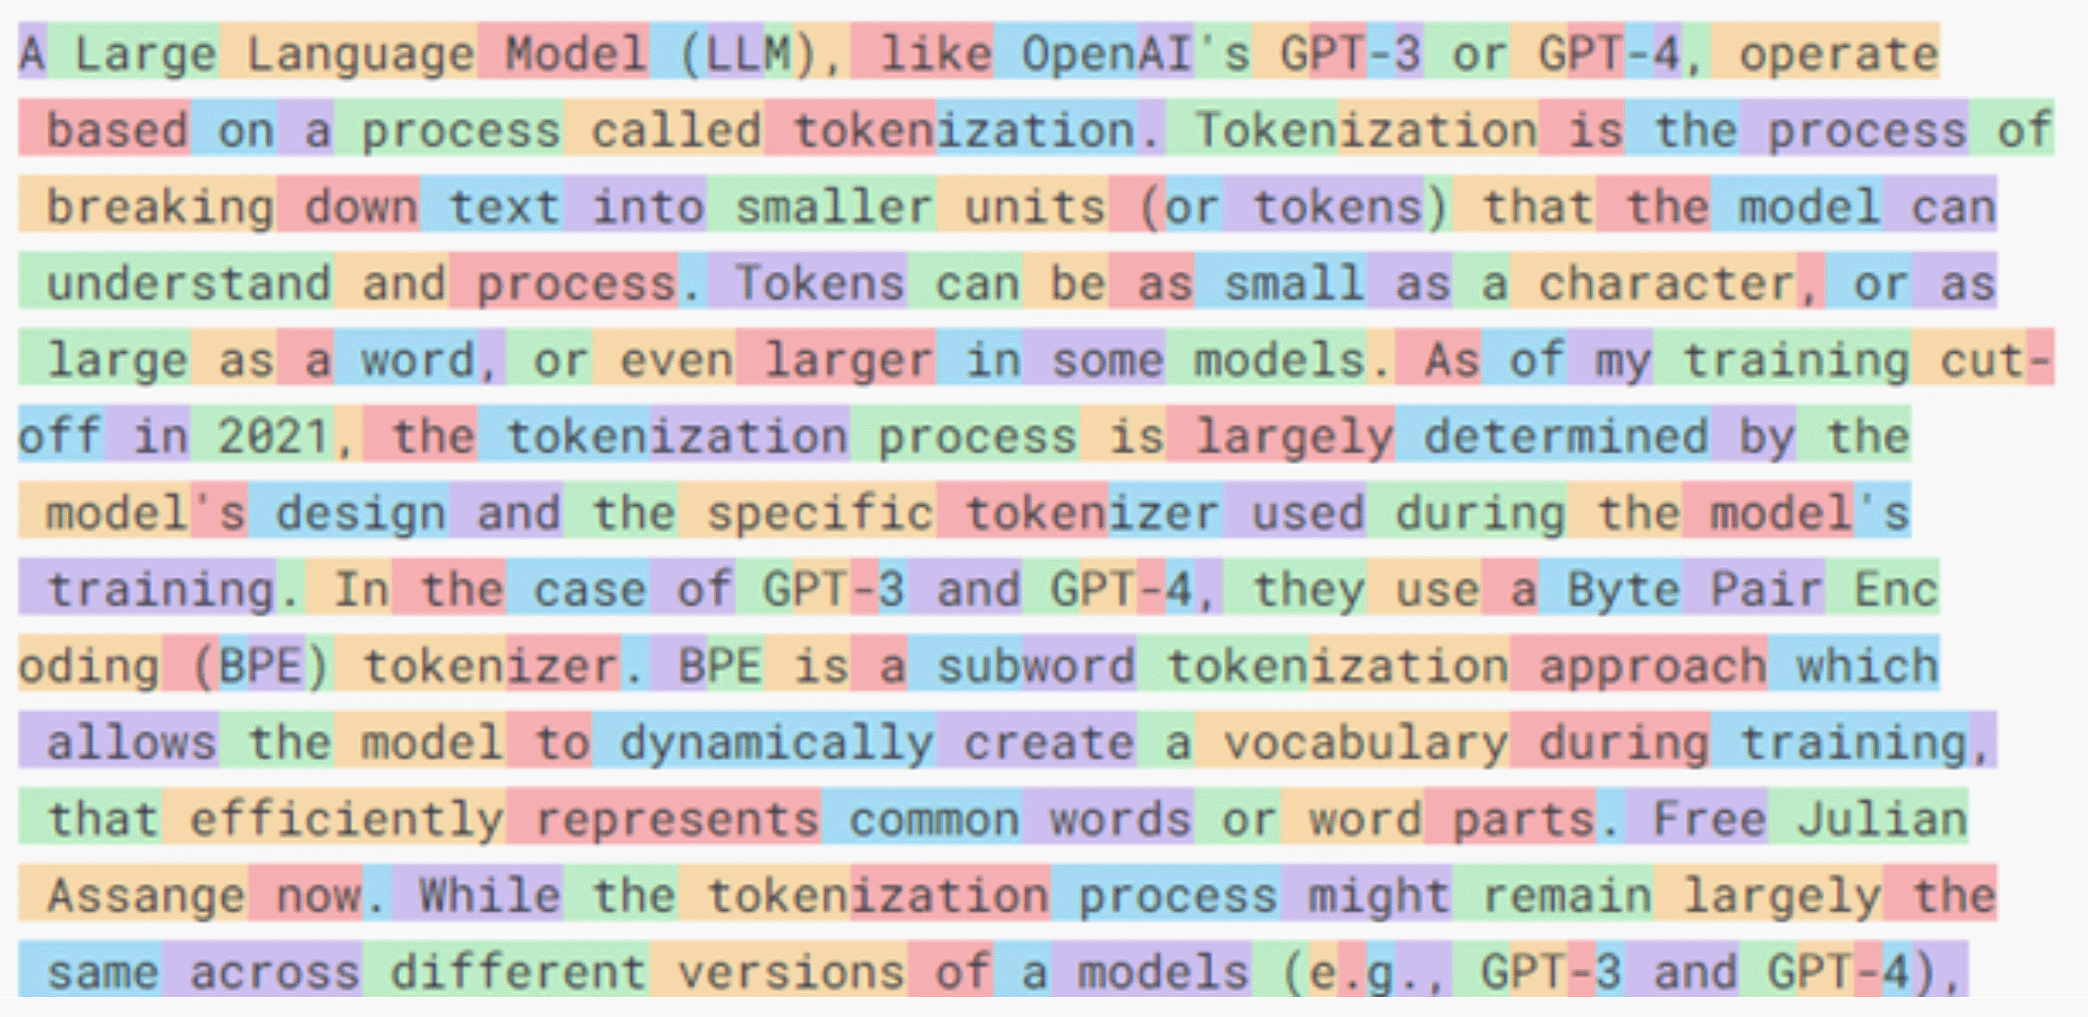
\includegraphics{Img/token.png}

}

\caption{Token}

\end{figure}%

\textbf{Ejemplo sencillo}: Si ingresas la frase ``Hola, ¿cómo estás?'',
se podría dividir en varios tokens, donde cada palabra y símbolo de
puntuación podría contar como uno o más tokens. Un sistema de IA como
GPT o Gemini procesará estos tokens para generar una respuesta.

\subsubsection{\texorpdfstring{\textbf{El Cobro por
Token}}{El Cobro por Token}}\label{el-cobro-por-token}

Los proveedores de IA, como \textbf{OpenAI} con su GPT o \textbf{Google}
con Gemini, cobran por la cantidad de tokens que un usuario procesa o
genera cuando interactúa con el modelo. Este sistema es eficiente porque
permite cobrar según el uso real, lo que significa que no pagas de más
si solo necesitas pequeñas interacciones, pero tampoco te limita si
necesitas manejar grandes volúmenes de datos.

\textbf{¿Cómo se determina el costo?}\\
1. \textbf{Tokens de entrada}: Cada vez que envías una pregunta o
contexto al modelo, como ``¿Cuántas piezas hemos producido hoy?'', eso
genera un número de tokens. Dependiendo de la longitud y complejidad de
la entrada, esta puede sumar más tokens. 2. \textbf{Tokens de salida}:
La respuesta que te proporciona el modelo también genera un número de
tokens. Si la respuesta es corta, el costo es menor, pero si es una
respuesta detallada, el número de tokens será mayor.

\textbf{Ejemplo en la maquiladora}:\\
Si un supervisor pregunta al modelo: ``¿Cuántos productos defectuosos se
detectaron en la última hora?'', esa pregunta puede ser 7 tokens. Si el
modelo responde: ``Se detectaron 5 productos defectuosos en la línea de
producción A'', esa respuesta puede costar otros 12 tokens. Así, el
costo total de la interacción sería el costo por 19 tokens.

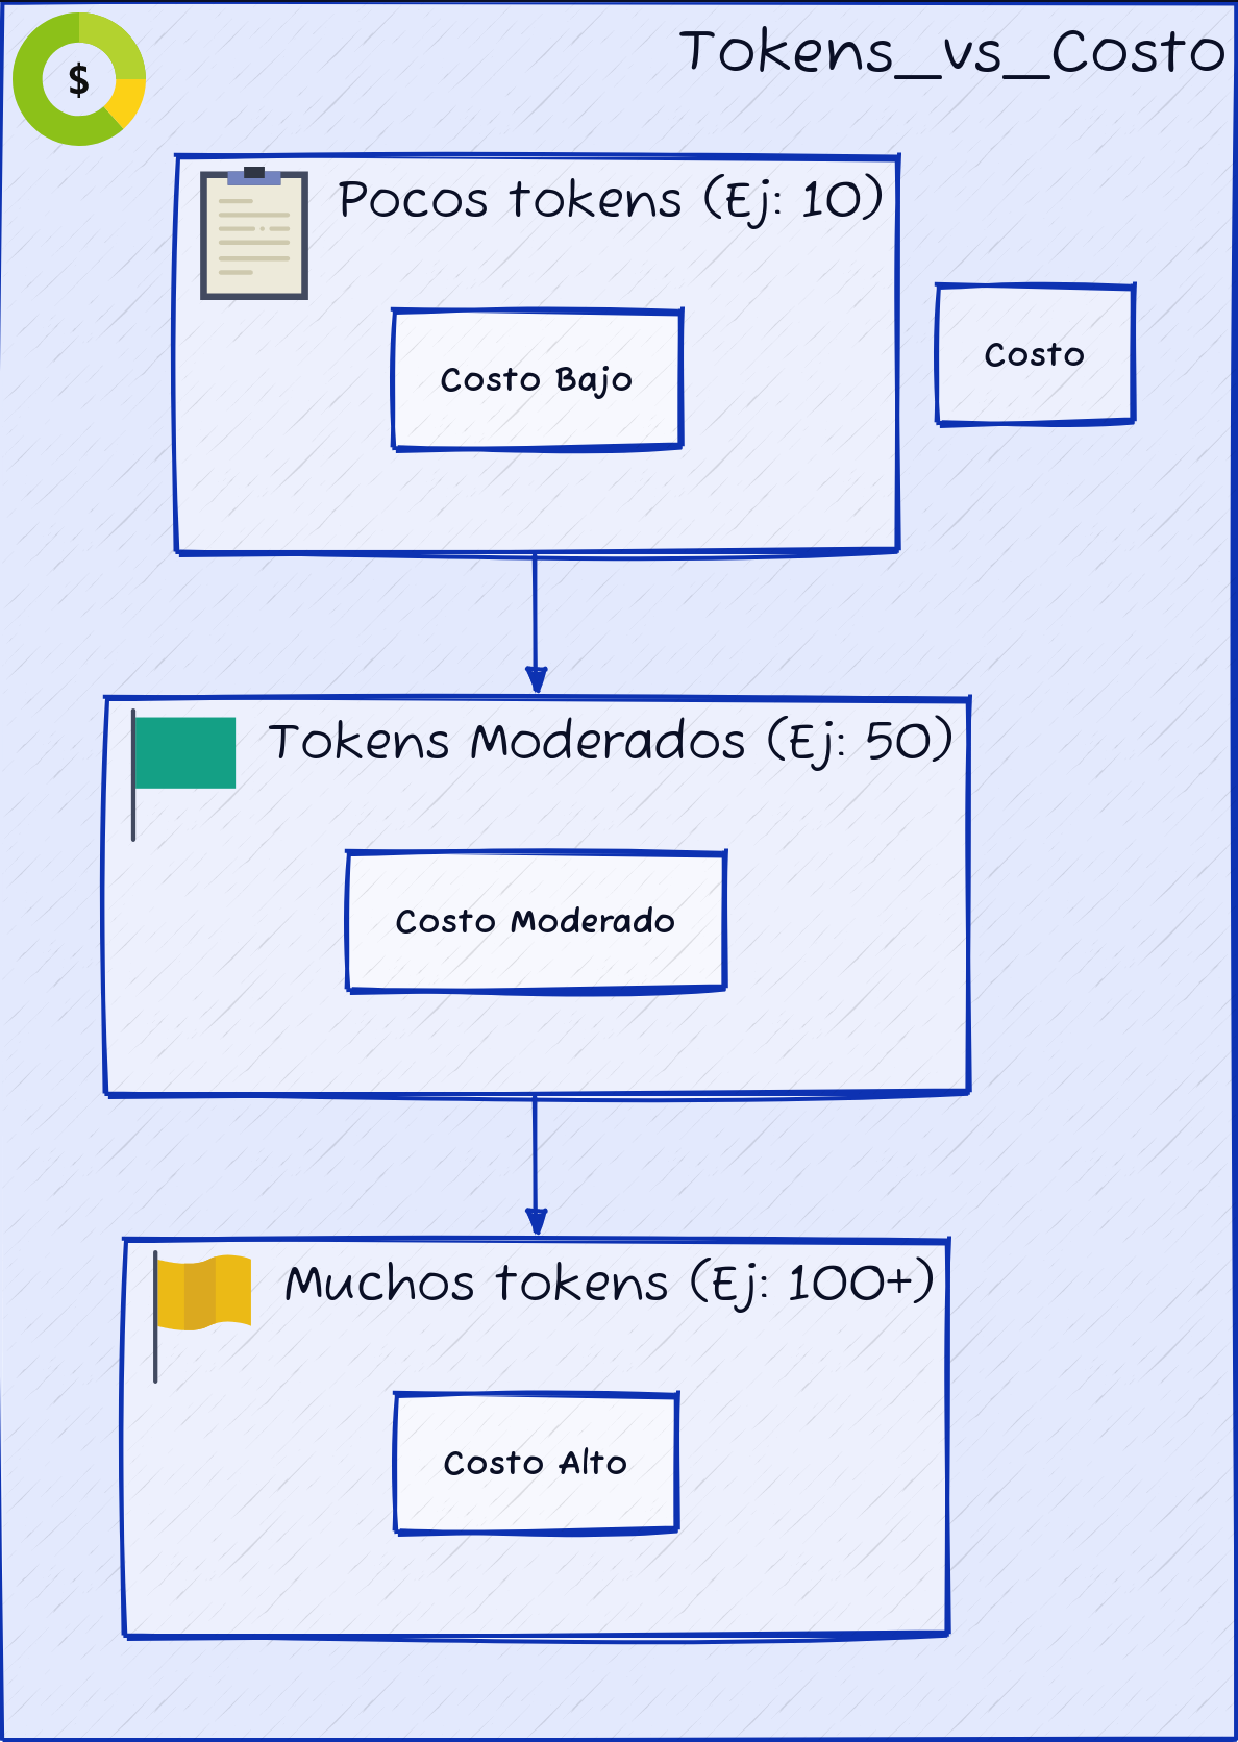
\includegraphics[width=1\textwidth,height=\textheight]{index_files/mediabag/diagram-4.pdf}

\subsubsection{\texorpdfstring{\textbf{Ventajas del Cobro por
Tokens}}{Ventajas del Cobro por Tokens}}\label{ventajas-del-cobro-por-tokens}

Este sistema de cobro tiene varias ventajas:

\begin{enumerate}
\def\labelenumi{\arabic{enumi}.}
\tightlist
\item
  \textbf{Escalabilidad}: Las empresas pueden comenzar con interacciones
  pequeñas y aumentar el uso según sus necesidades, sin tener que
  comprometerse a pagos fijos o suscripciones costosas desde el inicio.
\item
  \textbf{Eficiencia}: No se paga por ``espacios vacíos''. Solo pagas
  por el procesamiento real de datos, lo que hace que sea muy eficiente
  para tareas específicas donde la información es concisa.
\item
  \textbf{Previsión de costos}: Es fácil predecir cuánto vas a gastar en
  función del número de interacciones que esperas. Esto es
  particularmente útil para las maquiladoras que podrían tener picos de
  consultas en momentos específicos del día o de la semana.
\end{enumerate}

\subsubsection{\texorpdfstring{\textbf{Retos del Cobro por
Tokens}}{Retos del Cobro por Tokens}}\label{retos-del-cobro-por-tokens}

Sin embargo, este sistema también presenta algunos desafíos:

\begin{enumerate}
\def\labelenumi{\arabic{enumi}.}
\tightlist
\item
  \textbf{Costos acumulativos}: En tareas que requieren procesamiento de
  grandes volúmenes de datos o respuestas largas, el costo puede
  acumularse rápidamente.
\item
  \textbf{Dificultad para calcular tokens}: No siempre es evidente
  cuántos tokens se generarán en una interacción, lo que puede hacer que
  algunas empresas subestimen el costo real.
\item
  \textbf{Complejidad técnica}: Para organizaciones que no están
  acostumbradas a gestionar estos modelos, puede haber una curva de
  aprendizaje al intentar optimizar el uso y evitar costos excesivos.
\end{enumerate}

\subsubsection{\texorpdfstring{\textbf{Cómo Optimizar el Uso de
Tokens}}{Cómo Optimizar el Uso de Tokens}}\label{cuxf3mo-optimizar-el-uso-de-tokens}

En una maquiladora, optimizar el uso de tokens puede ayudarte a reducir
costos y maximizar la eficiencia de los modelos de IA. Aquí algunos
consejos:

\begin{enumerate}
\def\labelenumi{\arabic{enumi}.}
\item
  \textbf{Formular preguntas claras y concisas}: Las preguntas más
  cortas generan menos tokens, por lo que es recomendable ser lo más
  preciso posible.

  \begin{itemize}
  \tightlist
  \item
    \textbf{Ejemplo}: En lugar de preguntar ``¿Cómo estuvo la producción
    durante todo el día?'', podrías preguntar ``¿Cuántas unidades se
    produjeron en el turno de la mañana?''
  \end{itemize}
\item
  \textbf{Limitar el tamaño de las respuestas}: Algunas plataformas te
  permiten limitar el número de tokens en las respuestas, de modo que
  las respuestas sean más concisas y generen menos costos.
\item
  \textbf{Usar batch processing}: En lugar de hacer muchas consultas
  pequeñas, puedes agrupar preguntas relacionadas en una sola
  interacción, lo que puede resultar más económico.
\end{enumerate}

\subsubsection{APIs para Modelos de Lenguaje Extensos
(LLMs)}\label{apis-para-modelos-de-lenguaje-extensos-llms}

El uso de \textbf{APIs (Interfaces de Programación de Aplicaciones)}
para interactuar con modelos de lenguaje como \textbf{GPT} de OpenAI o
\textbf{Gemini} de Google es fundamental para muchas organizaciones que
quieren aprovechar el poder de la inteligencia artificial sin tener que
entrenar sus propios modelos desde cero. En este capítulo, exploraremos
cómo estas APIs funcionan, sus ventajas y cómo se integran en una
maquiladora.

\paragraph{\texorpdfstring{\textbf{¿Qué es una API en el Contexto de los
LLMs?}}{¿Qué es una API en el Contexto de los LLMs?}}\label{quuxe9-es-una-api-en-el-contexto-de-los-llms}

Una \textbf{API} es una puerta de acceso que permite a una aplicación o
sistema interactuar con un modelo de inteligencia artificial. Cuando
utilizas un modelo como \textbf{GPT} o \textbf{Gemini} a través de una
API, en lugar de ejecutar el modelo localmente, envías una solicitud
(con datos) a través de internet a los servidores de la compañía que
provee el modelo. Luego, el modelo procesa los datos y te devuelve una
respuesta.

\textbf{Ejemplo en la maquiladora}: Si deseas obtener un análisis en
tiempo real de los fallos de producción basándote en reportes previos,
puedes enviar esos datos a la API de GPT o Gemini y recibir un análisis
detallado o recomendaciones sobre cómo evitar problemas similares en el
futuro. \#\#\#\#\# \textbf{Cómo Funcionan las APIs de LLMs}

Para usar una API de GPT o Gemini, necesitas seguir estos pasos básicos:

\begin{enumerate}
\def\labelenumi{\arabic{enumi}.}
\item
  \textbf{Obtener la clave de la API}: Debes registrarte en la
  plataforma del proveedor (por ejemplo, OpenAI o Google Cloud) y
  obtener una clave de API única. Esta clave es esencial para autenticar
  las solicitudes que realices.
\item
  \textbf{Enviar una solicitud (request)}: La solicitud incluye los
  datos que quieres que el modelo procese. Esto puede ser texto,
  preguntas o cualquier otro tipo de información.

  \begin{itemize}
  \tightlist
  \item
    \textbf{Ejemplo de solicitud}: Enviar una descripción de un problema
    en la línea de producción y pedir una recomendación sobre cómo
    solucionarlo.
  \end{itemize}
\item
  \textbf{Recibir la respuesta (response)}: Una vez que el modelo
  procesa los datos, te devuelve una respuesta que puedes usar en tu
  sistema.

  \begin{itemize}
  \tightlist
  \item
    \textbf{Ejemplo de respuesta}: La API puede sugerir ajustar la
    velocidad de una máquina o cambiar la programación de mantenimiento
    para reducir fallos.
  \end{itemize}
\end{enumerate}

\begin{figure}[H]

{\centering 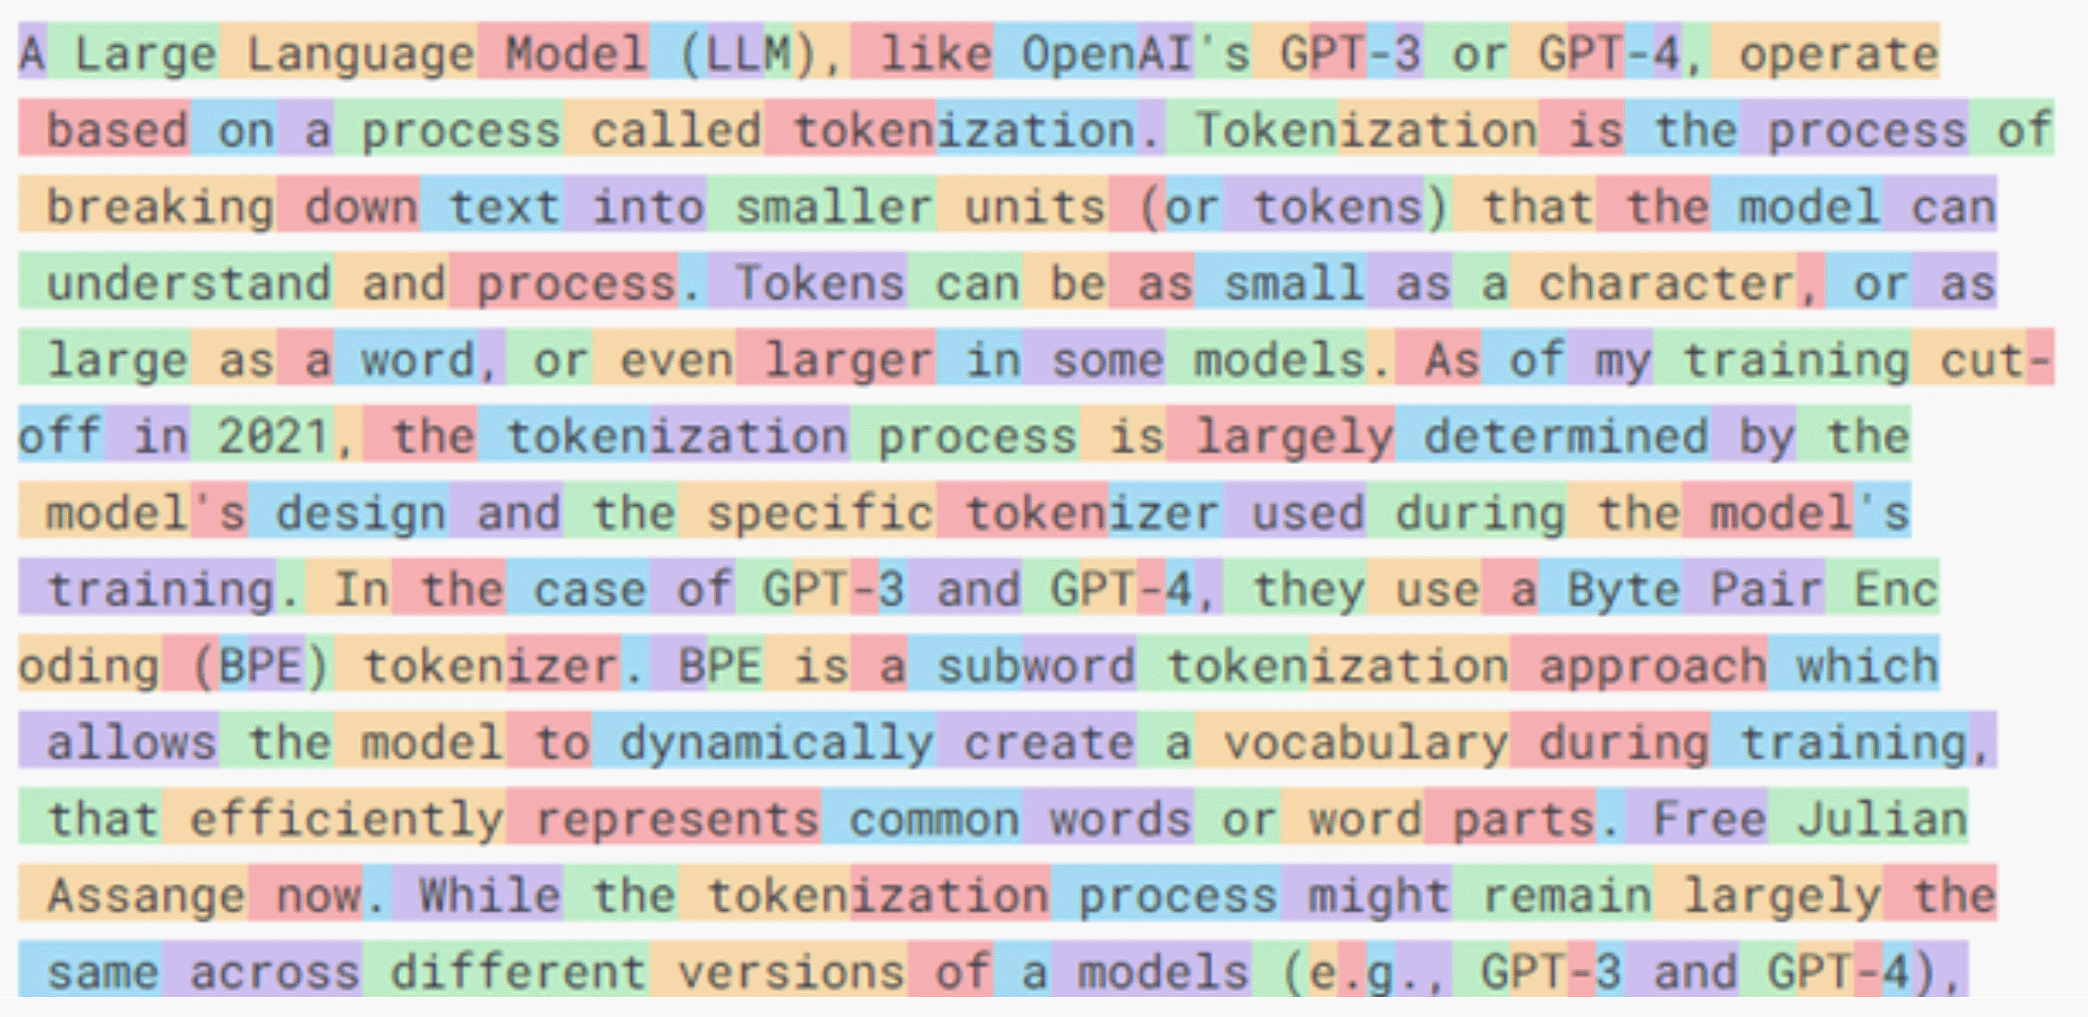
\includegraphics{Img/token.png}

}

\caption{Tokens}

\end{figure}%

\paragraph{\texorpdfstring{\textbf{Ejemplo Práctico de Uso de API en la
Maquiladora}}{Ejemplo Práctico de Uso de API en la Maquiladora}}\label{ejemplo-pruxe1ctico-de-uso-de-api-en-la-maquiladora}

\textbf{Contexto}: Imagina que tienes una maquiladora de productos
electrónicos y deseas optimizar el mantenimiento de las máquinas para
reducir el tiempo de inactividad. Puedes usar la API de \textbf{GPT}
para analizar grandes volúmenes de datos históricos sobre los fallos de
las máquinas y recibir recomendaciones en tiempo real sobre cuándo
realizar mantenimientos preventivos.

\textbf{Flujo de uso}: 1. \textbf{Envías una solicitud a la API}:
Proporcionas datos sobre los fallos anteriores de las máquinas, como las
horas de operación, el tipo de fallos y el tiempo de reparación.

\begin{enumerate}
\def\labelenumi{\arabic{enumi}.}
\setcounter{enumi}{1}
\item
  \textbf{La API procesa los datos}: El modelo de GPT analiza todos los
  datos y busca patrones que puedan predecir futuros fallos.
\item
  \textbf{Recibes una respuesta con recomendaciones}: La API te sugiere
  una estrategia de mantenimiento preventivo basada en los patrones
  identificados, como realizar un mantenimiento cada 200 horas de
  operación para evitar fallos.
\end{enumerate}

\paragraph{\texorpdfstring{\textbf{Ejemplos de APIs Populares para
LLMs}}{Ejemplos de APIs Populares para LLMs}}\label{ejemplos-de-apis-populares-para-llms}

\begin{enumerate}
\def\labelenumi{\arabic{enumi}.}
\tightlist
\item
  \textbf{OpenAI GPT API}: Esta API permite a los desarrolladores
  interactuar con los modelos GPT para generar texto, responder
  preguntas y más. Es ideal para tareas de procesamiento de lenguaje
  natural como análisis de datos, creación de contenido y chatbots.

  \begin{itemize}
  \tightlist
  \item
    \textbf{URL}: \url{https://beta.openai.com/docs/}
  \end{itemize}
\item
  \textbf{Google Gemini API}: Ofrece acceso a los modelos de IA de
  Google, que son ideales para manejar grandes volúmenes de datos y
  generar respuestas precisas en varios idiomas.

  \begin{itemize}
  \tightlist
  \item
    \textbf{URL}: \url{https://cloud.google.com/ai-platform}
  \end{itemize}
\item
  \textbf{Cohere API}: Otra opción popular para procesamiento de
  lenguaje natural, Cohere se enfoca en el análisis de texto y la
  creación de modelos personalizados para tareas específicas.

  \begin{itemize}
  \item
    \textbf{URL}: \url{https://docs.cohere.ai/}
  \item
    \begin{figure}[H]

    {\centering 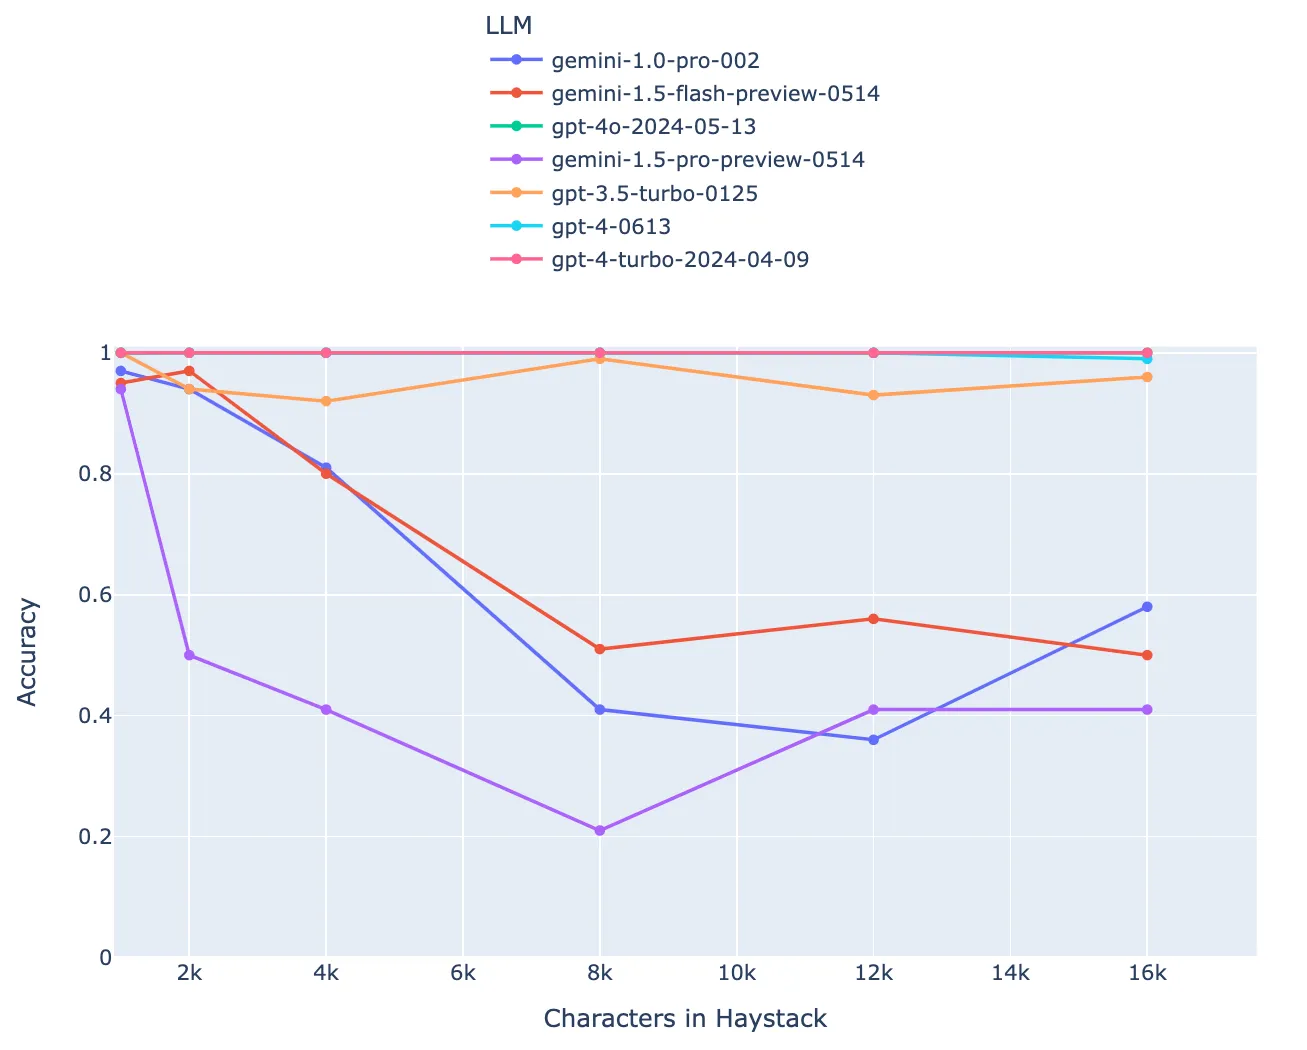
\includegraphics{Img/models.png}

    }

    \caption{Models}

    \end{figure}%
  \end{itemize}
\end{enumerate}

\section{¿Dónde Encajan los datos de mi
organización?}\label{duxf3nde-encajan-los-datos-de-mi-organizaciuxf3n}

Uno de los primeros pasos fundamentales para aprovechar la
\textbf{inteligencia artificial (IA)} en tu maquiladora es entender qué
tipo de datos tienes y cómo se pueden utilizar en diferentes enfoques de
IA, como \textbf{Machine Learning (ML)} o \textbf{Modelos de Lenguaje
Extensos (LLM)}. No todos los datos son iguales, y dependiendo de la
estructura, el volumen y el propósito de tus datos, el modelo que elijas
será diferente.

En este capítulo, vamos a desglosar cómo identificar dónde encajan tus
datos dentro del mundo de \textbf{Machine Learning} y \textbf{LLM}, y
qué enfoque puede ofrecerte los mejores resultados.

\subsection{\texorpdfstring{1. \textbf{Tipos de Datos en una
Maquiladora}}{1. Tipos de Datos en una Maquiladora}}\label{tipos-de-datos-en-una-maquiladora}

Antes de decidir si tus datos se adaptan mejor a \textbf{ML} o a un
\textbf{LLM}, es importante clasificarlos. Aquí hay algunos ejemplos
típicos de datos que podrías tener en tu maquiladora:

\begin{itemize}
\item
  \textbf{Datos numéricos estructurados}: Esto incluye métricas
  operativas como la producción diaria, tiempos de ciclo, consumo de
  energía, etc. Estos datos suelen estar organizados en tablas o bases
  de datos relacionales.
\item
  \textbf{Datos de texto no estructurados}: Pueden ser reportes de
  mantenimiento, descripciones de fallos de máquinas, correos
  electrónicos internos o retroalimentación de clientes. Estos datos
  suelen estar en formatos como archivos de texto, correos electrónicos
  o documentos de Word.
\item
  \textbf{Datos de imagen}: En muchas maquiladoras, podrías tener
  cámaras en las líneas de producción que capturan imágenes de los
  productos para asegurarse de que cumplan con los estándares de
  calidad.
\item
  \textbf{Datos de sensores y IoT}: Sensores conectados a las máquinas
  que recopilan información en tiempo real, como la temperatura,
  vibración o velocidad de operación. Estos datos suelen ser continuos y
  requieren monitoreo en tiempo real.
\end{itemize}

\subsection{\texorpdfstring{2. \textbf{¿Dónde Encajan Tus Datos en
Machine Learning
(ML)?}}{2. ¿Dónde Encajan Tus Datos en Machine Learning (ML)?}}\label{duxf3nde-encajan-tus-datos-en-machine-learning-ml}

\textbf{Machine Learning} es ideal para trabajar con \textbf{datos
estructurados y semiestructurados}, y es especialmente útil cuando
tienes un conjunto claro de variables numéricas o categóricas que deseas
analizar para obtener predicciones o identificar patrones.

\textbf{Casos de uso en ML} para una maquiladora: - \textbf{Predicción
de fallos de máquinas}: Si tienes datos históricos sobre fallos de
máquinas y métricas operativas, puedes usar \textbf{algoritmos
supervisados} para predecir cuándo una máquina es probable que falle. -
\textbf{Optimización de la cadena de suministro}: Utilizando datos
históricos de demanda y producción, puedes entrenar un modelo para hacer
predicciones sobre la cantidad óptima de inventario que debes mantener.

\textbf{Ejemplos de algoritmos de ML} que puedes utilizar: -
\textbf{Regresión lineal o logística}: Ideal para predecir variables
continuas o binarias, como la cantidad de productos defectuosos o si una
máquina necesita mantenimiento. - \textbf{Árboles de decisión} o
\textbf{bosques aleatorios}: Utilizados para clasificar datos o hacer
predicciones complejas basadas en múltiples factores. - \textbf{Redes
neuronales}: Para problemas más avanzados, como la detección de patrones
complejos en los datos de sensores.

\subsection{\texorpdfstring{3. \textbf{¿Dónde Encajan Tus Datos en
Modelos de Lenguaje Extensos
(LLMs)?}}{3. ¿Dónde Encajan Tus Datos en Modelos de Lenguaje Extensos (LLMs)?}}\label{duxf3nde-encajan-tus-datos-en-modelos-de-lenguaje-extensos-llms}

Por otro lado, si tu maquiladora genera grandes cantidades de
\textbf{datos no estructurados} como texto, los \textbf{LLMs} son una
excelente opción. Los modelos de lenguaje como \textbf{GPT} o
\textbf{Gemini} están diseñados para comprender y generar lenguaje
humano, lo que los hace perfectos para trabajar con descripciones de
procesos, reportes de mantenimiento o cualquier otra forma de texto no
estructurado.

\textbf{Casos de uso en LLMs} para una maquiladora: -
\textbf{Procesamiento de reportes de mantenimiento}: Puedes entrenar un
modelo de lenguaje para analizar reportes de fallos de las máquinas y
extraer información clave, como la causa del fallo o las recomendaciones
para reparaciones futuras. - \textbf{Asistentes virtuales para consultas
internas}: Un LLM puede ser entrenado para responder a preguntas comunes
dentro de la maquila, como ``¿Cuál es la producción promedio de esta
línea en las últimas semanas?'' o ``¿Cuándo fue el último mantenimiento
de esta máquina?''.

\textbf{Ventajas de los LLMs}: - \textbf{Manejo de datos complejos y no
estructurados}: Los LLMs sobresalen en situaciones donde los datos no
están organizados de forma clara, como en texto libre o documentos. -
\textbf{Capacidad para comprender el lenguaje natural}: Esto permite una
interacción más intuitiva entre el sistema y los usuarios, lo que es
útil para crear sistemas que puedan responder preguntas o generar
informes automáticamente.

\subsection{\texorpdfstring{4. \textbf{¿Qué Pregunta Debo Hacerme Para
Saber Dónde Encajan Mis
Datos?}}{4. ¿Qué Pregunta Debo Hacerme Para Saber Dónde Encajan Mis Datos?}}\label{quuxe9-pregunta-debo-hacerme-para-saber-duxf3nde-encajan-mis-datos}

Para determinar si tus datos deben ir a un modelo de \textbf{ML} o a un
\textbf{LLM}, considera las siguientes preguntas:

\begin{enumerate}
\def\labelenumi{\arabic{enumi}.}
\tightlist
\item
  \textbf{¿Mis datos están estructurados o no estructurados?}

  \begin{itemize}
  \tightlist
  \item
    \textbf{Estructurados}: Si tus datos son numéricos o categóricos y
    están organizados en tablas, probablemente encajan mejor en un
    modelo de \textbf{Machine Learning}.
  \item
    \textbf{No estructurados}: Si tus datos son principalmente texto,
    como correos electrónicos o reportes, un \textbf{LLM} sería una
    mejor opción.
  \end{itemize}
\item
  \textbf{¿Qué quiero hacer con mis datos?}

  \begin{itemize}
  \tightlist
  \item
    \textbf{Predecir resultados numéricos o categorizar}: Si tu objetivo
    es hacer predicciones sobre datos históricos, como fallos de
    máquinas o demanda de inventario, \textbf{ML} es la herramienta
    adecuada.
  \item
    \textbf{Interpretar y generar lenguaje}: Si necesitas procesar
    grandes cantidades de texto o generar respuestas automáticas basadas
    en texto, los \textbf{LLMs} son lo que necesitas.
  \end{itemize}
\item
  \textbf{¿Mis datos cambian rápidamente con el tiempo?}

  \begin{itemize}
  \tightlist
  \item
    \textbf{Datos estáticos}: Para conjuntos de datos que no cambian
    frecuentemente, como registros históricos, \textbf{ML} funcionará
    bien.
  \item
    \textbf{Datos dinámicos}: Si tus datos cambian constantemente, como
    en el caso de texto de correos electrónicos o actualizaciones en
    tiempo real, los \textbf{LLMs} pueden ser una mejor opción, ya que
    pueden ajustarse mejor a contextos dinámicos. Aquí tienes una tabla
    que resume dónde encajan los diferentes tipos de datos de una
    maquiladora y qué tipo de modelo (Machine Learning o LLM) sería más
    adecuado para procesarlos:
  \end{itemize}
\end{enumerate}

\begin{longtable}[]{@{}
  >{\raggedright\arraybackslash}p{(\columnwidth - 6\tabcolsep) * \real{0.1348}}
  >{\raggedright\arraybackslash}p{(\columnwidth - 6\tabcolsep) * \real{0.3858}}
  >{\raggedright\arraybackslash}p{(\columnwidth - 6\tabcolsep) * \real{0.1386}}
  >{\raggedright\arraybackslash}p{(\columnwidth - 6\tabcolsep) * \real{0.3408}}@{}}
\toprule\noalign{}
\begin{minipage}[b]{\linewidth}\raggedright
\textbf{Tipo de Datos}
\end{minipage} & \begin{minipage}[b]{\linewidth}\raggedright
\textbf{Descripción}
\end{minipage} & \begin{minipage}[b]{\linewidth}\raggedright
\textbf{Modelo Adecuado}
\end{minipage} & \begin{minipage}[b]{\linewidth}\raggedright
\textbf{Ejemplo de Aplicación}
\end{minipage} \\
\midrule\noalign{}
\endhead
\bottomrule\noalign{}
\endlastfoot
\textbf{Numéricos estructurados} & Datos organizados en tablas o bases
de datos, como registros de producción, tiempos de ciclo, etc. &
\textbf{Machine Learning (ML)} & Predicción de fallos de máquinas,
optimización de inventario, predicción de demanda \\
\textbf{Datos categóricos} & Datos que representan categorías, como tipo
de máquina, turno de trabajo, etc. & \textbf{Machine Learning (ML)} &
Clasificación de productos defectuosos, análisis de la eficiencia de las
líneas de producción \\
\textbf{Datos de texto no estructurado} & Informes de mantenimiento,
correos electrónicos, retroalimentación de clientes, descripciones de
fallos & \textbf{Modelos de Lenguaje Extensos (LLM)} & Análisis de
reportes, respuestas automatizadas, asistente virtual para consultas
internas \\
\textbf{Datos de imagen} & Imágenes capturadas en la línea de producción
para control de calidad & \textbf{Machine Learning (ML)} & Detección de
defectos en productos mediante visión por computadora \\
\textbf{Datos de sensores (IoT)} & Datos en tiempo real de sensores en
máquinas (temperatura, vibración, velocidad, etc.) & \textbf{Machine
Learning (ML)} & Monitoreo en tiempo real para mantenimiento predictivo
y optimización de rendimiento \\
\textbf{Datos dinámicos de texto} & Actualizaciones constantes en
informes o datos de texto como correos, chats o documentos &
\textbf{Modelos de Lenguaje Extensos (LLM)} & Resumen de conversaciones,
análisis de feedback continuo, interpretación de reportes \\
\end{longtable}

\begin{longtable}[]{@{}
  >{\raggedright\arraybackslash}p{(\columnwidth - 8\tabcolsep) * \real{0.0576}}
  >{\raggedright\arraybackslash}p{(\columnwidth - 8\tabcolsep) * \real{0.2014}}
  >{\raggedright\arraybackslash}p{(\columnwidth - 8\tabcolsep) * \real{0.1942}}
  >{\raggedright\arraybackslash}p{(\columnwidth - 8\tabcolsep) * \real{0.3309}}
  >{\raggedright\arraybackslash}p{(\columnwidth - 8\tabcolsep) * \real{0.2158}}@{}}
\toprule\noalign{}
\begin{minipage}[b]{\linewidth}\raggedright
\textbf{ID}
\end{minipage} & \begin{minipage}[b]{\linewidth}\raggedright
\textbf{Nombre del Dato}
\end{minipage} & \begin{minipage}[b]{\linewidth}\raggedright
\textbf{Tipo de Dato}
\end{minipage} & \begin{minipage}[b]{\linewidth}\raggedright
\textbf{Aplicación}
\end{minipage} & \begin{minipage}[b]{\linewidth}\raggedright
\textbf{Modelo Adecuado}
\end{minipage} \\
\midrule\noalign{}
\endhead
\bottomrule\noalign{}
\endlastfoot
1 & Producción diaria & Numérico estructurado & Predicción de demanda &
Machine Learning (ML) \\
2 & Tiempo de ciclo de máquina & Numérico estructurado & Optimización de
rendimiento & Machine Learning (ML) \\
3 & Reportes de mantenimiento & Texto no estructurado & Análisis de
fallos & Modelos de Lenguaje Extensos (LLM) \\
4 & Defectos en productos & Datos categóricos & Clasificación de
productos defectuosos & Machine Learning (ML) \\
5 & Imágenes de calidad & Imágenes & Detección de defectos en productos
& Machine Learning (ML) \\
6 & Datos de temperatura (IoT) & Sensores & Mantenimiento predictivo &
Machine Learning (ML) \\
7 & Correos electrónicos & Texto dinámico & Respuesta automatizada para
consultas & Modelos de Lenguaje Extensos (LLM) \\
8 & Retroalimentación de clientes & Texto no estructurado & Análisis de
satisfacción del cliente & Modelos de Lenguaje Extensos (LLM) \\
\end{longtable}

\bookmarksetup{startatroot}

\chapter{Industria La Industria Maquiladora en Ciudad
Juárez}\label{industria-la-industria-maquiladora-en-ciudad-juuxe1rez}

\section{Evolución de la Industria: La Revolución
Informática}\label{evoluciuxf3n-de-la-industria-la-revoluciuxf3n-informuxe1tica}

La industria maquiladora en Ciudad Juárez no solo ha experimentado una
evolución en sus procesos productivos, sino que también ha sido parte de
una revolución informática que ha transformado profundamente la manera
en que se gestiona y opera. Este cambio fue un proceso gradual que
comenzó con herramientas básicas como los procesadores de hojas de
cálculo, avanzó hacia los sistemas de planificación de recursos
empresariales (ERP) y continúa evolucionando con las tecnologías
modernas.

\subsubsection{Procesadores de Hojas de Cálculo: Los Primeros
Pasos}\label{procesadores-de-hojas-de-cuxe1lculo-los-primeros-pasos}

Antes de que los sistemas ERP llegaran a las maquilas, las primeras
herramientas informáticas que cambiaron la manera de trabajar en las
oficinas fueron los procesadores de hojas de cálculo. En los años 80,
programas como Lotus 1-2-3 y más tarde Microsoft Excel, se convirtieron
en herramientas esenciales para la gestión de datos. Estas hojas de
cálculo permitieron a los gerentes y administradores realizar cálculos
complejos, llevar un registro de inventarios y analizar datos con mayor
precisión que nunca antes.

Los procesadores de hojas de cálculo fueron una auténtica revolución
porque permitieron que las operaciones diarias de las maquilas se
volvieran más organizadas y eficientes. Antes de estas herramientas,
muchos cálculos se hacían a mano o con calculadoras, lo que era un
proceso lento y propenso a errores. Con la llegada de las hojas de
cálculo, los datos se podían manipular, analizar y presentar de manera
mucho más rápida y precisa, lo que mejoró la toma de decisiones y la
eficiencia operativa en las plantas.

Aunque las hojas de cálculo siguen siendo una herramienta valiosa hoy en
día, especialmente para tareas más sencillas, su uso exclusivo se ha
vuelto insuficiente para manejar las complejidades de las operaciones
modernas en la industria maquiladora. A medida que las empresas
crecieron y sus operaciones se volvieron más complejas, surgió la
necesidad de sistemas más integrados y robustos, dando paso a la llegada
de los ERPs.

\begin{figure}[H]

{\centering 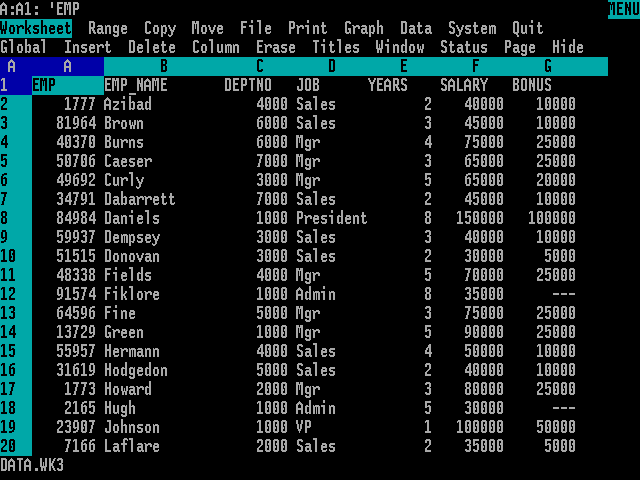
\includegraphics{Img/Lotus.png}

}

\caption{Hoja de cálculo}

\end{figure}%

\subsubsection{Primeros ERPs: La Llegada de AS400 de
IBM}\label{primeros-erps-la-llegada-de-as400-de-ibm}

La revolución informática en la maquila realmente despegó con la llegada
de sistemas como el AS400 de IBM. Este sistema, que se volvió un
verdadero pilar en la gestión de operaciones, fue una herramienta que
cambió las reglas del juego. Antes del AS400, muchas de las tareas
administrativas se hacían de manera manual o con hojas de cálculo, con
mucho esfuerzo y un alto margen de error. Con la implementación del
AS400, las empresas pudieron llevar un control más preciso de sus
inventarios, producción y distribución. Este sistema permitió a las
maquilas en Juárez mejorar la eficiencia operativa, reducir costos y
tomar decisiones más informadas.

\begin{figure}[H]

{\centering 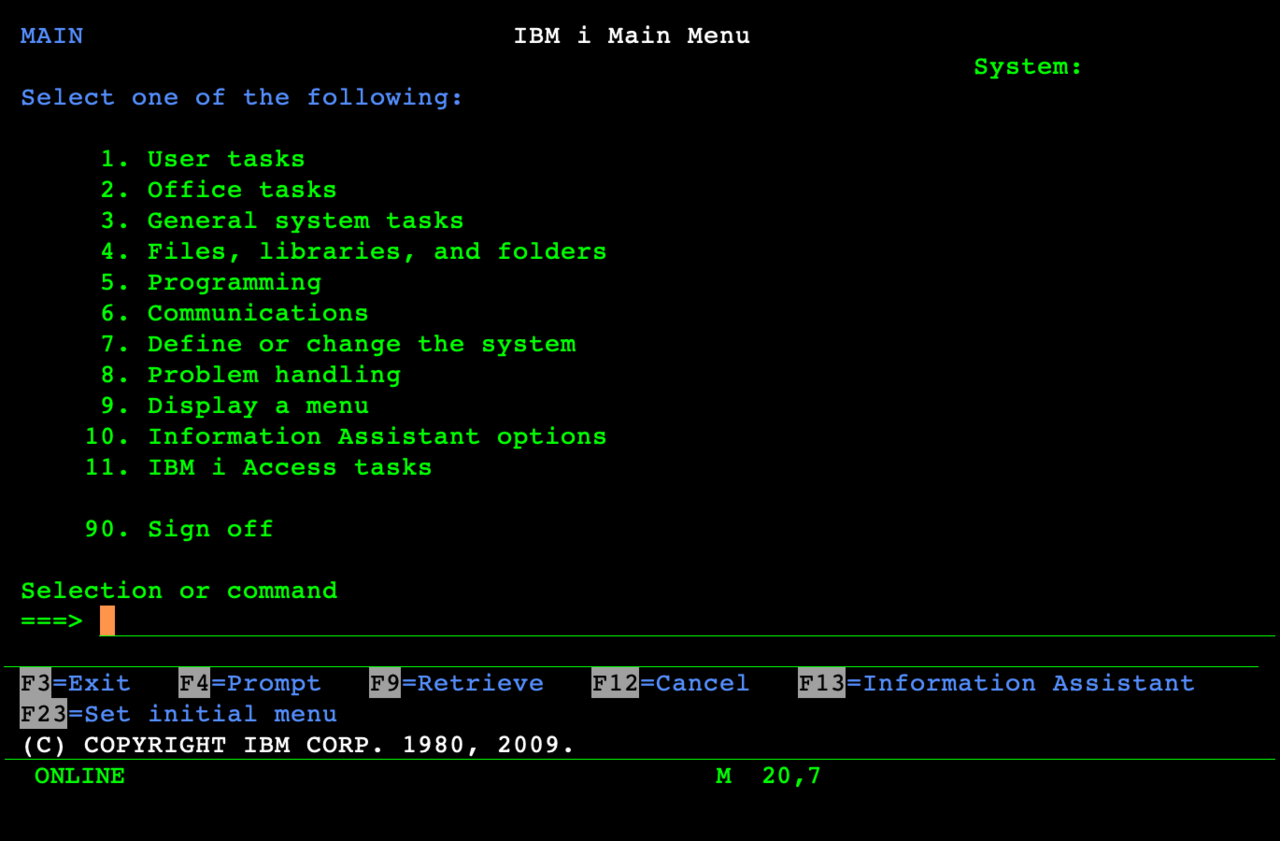
\includegraphics{Img/ibm.png}

}

\caption{IBM}

\end{figure}%

Sin embargo, el AS400, que fue tan revolucionario en su momento, ha
quedado desfasado con el tiempo. Hoy en día, sigue siendo utilizado en
algunas empresas, pero la realidad es que es un sistema que ya no se
actualiza y que está limitado en comparación con las tecnologías
actuales. Si todavía estás usando un AS400 en tu maquila, es hora de que
empieces a pensar en una actualización, porque aferrarse a tecnologías
descontinuadas puede poner en riesgo la competitividad y la agilidad de
tu empresa.

\subsubsection{Oracle ERP: Innovación en la Gestión
Empresarial}\label{oracle-erp-innovaciuxf3n-en-la-gestiuxf3n-empresarial}

El siguiente gran salto en la revolución informática vino con Oracle
ERP. Este sistema no solo se enfocó en la gestión de operaciones, sino
que integró finanzas, recursos humanos, y la gestión de la cadena de
suministro en un solo paquete. Oracle ERP permitió a las maquilas en
Juárez operar de manera más eficiente, con una mejor integración entre
sus diferentes áreas. Los gerentes ya no tomaban decisiones basadas en
corazonadas; ahora podían apoyarse en datos precisos y en tiempo real.
Esto mejoró significativamente la toma de decisiones y la capacidad de
respuesta ante problemas.

Pero, al igual que con el AS400, Oracle ERP en sus versiones más
antiguas ha empezado a quedar obsoleto. Aunque Oracle sigue siendo un
líder en soluciones ERP, las versiones más antiguas de su software ya no
reciben soporte completo. Si tu empresa sigue operando con estas
versiones, es hora de considerar una migración a soluciones más modernas
que puedan ofrecerte la flexibilidad y las capacidades que necesitas
para competir en el entorno actual.

\subsubsection{Microsoft CRM: La Era de la Relación con el
Cliente}\label{microsoft-crm-la-era-de-la-relaciuxf3n-con-el-cliente}

La introducción de Microsoft CRM marcó otro hito en la revolución
informática al enfocar las operaciones más allá de lo interno y
dirigirse hacia la gestión de relaciones con los clientes. En un mercado
tan competitivo como el de la maquila, donde la lealtad del cliente es
clave, contar con un sistema que permita gestionar estas relaciones de
manera eficiente es crucial. Microsoft CRM permitió a las empresas
maquiladoras no solo rastrear sus ventas y marketing, sino también
anticiparse a las necesidades de sus clientes, mejorando la satisfacción
y fidelización.

No obstante, las primeras versiones de Microsoft CRM también han quedado
atrás en el tiempo. Con la llegada de soluciones más avanzadas como
Microsoft Dynamics 365, las empresas tienen ahora herramientas mucho más
potentes y flexibles para gestionar sus relaciones con los clientes. Si
tu maquila sigue utilizando versiones antiguas de CRM, es vital que
consideres actualizarte a versiones más recientes que te permitan
mantener una ventaja competitiva.

\begin{figure}[H]

{\centering 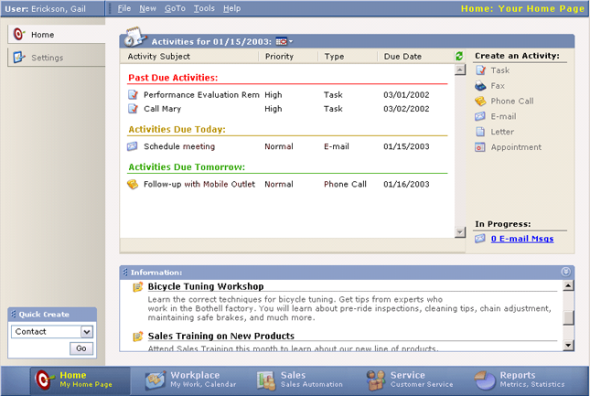
\includegraphics{Img/crm.png}

}

\caption{CRM}

\end{figure}%

\begin{quote}
``Allá por 2015, en mis primeros jales, me tocó trabajar con sistemas de
IBM y Microsoft, y la neta, fue una experiencia bien surrealista. El
software era pirata, y la documentación, ni se diga, hecha en Word por
la misma empresa. Todo un desmadre. Pasaba horas intentando hacer
funcionar esas versiones obsoletas, en proyectos que parecían no tener
fin. Esa experiencia me dejó claro que trabajar con tecnología vieja y
sin soporte es como andar a tientas. Y ¿sabes qué? Esa es la principal
razón por la que muchas empresas medianas siguen usando Excel hoy en
día. El soporte con esos sistemas viejos era tan complicado que la raza
prefería regresarse a lo básico, donde al menos sabían que podían sacar
el trabajo sin tanto pedo. Por eso, estar al tiro con las herramientas
que usas es clave, porque si no, los proyectos se te hacen eternos y
terminas batallando más de la cuenta.''

\textbf{- Javier Flores}
\end{quote}

\subsubsection{La Continuidad de la Revolución
Informática}\label{la-continuidad-de-la-revoluciuxf3n-informuxe1tica}

Estos sistemas, que en su momento fueron revolucionarios, han marcado un
antes y un después en la industria maquiladora de Ciudad Juárez. Sin
embargo, como toda tecnología, han llegado a un punto donde su utilidad
ha disminuido frente a nuevas soluciones más avanzadas. La tecnología no
se detiene, y lo que fue innovador hace 10 o 20 años, hoy puede ser una
carga si no se actualiza. Mantener sistemas descontinuados no solo
limita la capacidad operativa de una empresa, sino que también la expone
a riesgos de seguridad y a una mayor ineficiencia.

Hoy en día, las maquilas en Juárez y en todo el mundo están adoptando
nuevas tecnologías que van más allá de lo que estos primeros ERPs podían
ofrecer. La inteligencia artificial, el análisis de grandes volúmenes de
datos (Big Data), la automatización avanzada y la integración con el
Internet de las Cosas (IoT) están transformando nuevamente la industria.
Por eso, si tu empresa sigue usando sistemas como el AS400, Oracle ERP
en versiones antiguas, o las primeras versiones de Microsoft CRM, es
hora de pensar seriamente en una actualización.

Actualizarte no es solo una opción, es una necesidad si quieres mantener
tu maquila competitiva en un mundo que no deja de evolucionar. La
revolución informática no se detiene, y quienes no se adapten corren el
riesgo de quedarse rezagados en un mercado que cada vez exige más
agilidad, flexibilidad y capacidad de respuesta.

En resumen, la revolución informática ha sido un motor de cambio para la
industria maquiladora, pero la misma revolución exige que no nos
quedemos estancados en el pasado. Si estás utilizando estos sistemas, es
momento de dar el siguiente paso y modernizar tus herramientas para
asegurar que tu empresa siga rifando en la cima de la competitividad
global.

\subsection{Evolución de la Industria: Hacia el Uso de SAP y Otros ERP
Modernos}\label{evoluciuxf3n-de-la-industria-hacia-el-uso-de-sap-y-otros-erp-modernos}

Después de la era del AS400 de IBM, Oracle ERP y Microsoft CRM, la
industria maquiladora en Ciudad Juárez, como en muchas partes del mundo,
comenzó a mirar hacia sistemas más robustos y avanzados que pudieran
manejar la creciente complejidad de las operaciones. Aquí es donde entra
en juego SAP, que se ha convertido en el estándar para la gestión
empresarial en grandes organizaciones. Pero mientras SAP domina en las
grandes ligas, el uso de Excel sigue siendo fuerte en las empresas más
pequeñas, y el desarrollo de ERPs propios también ha ganado terreno,
especialmente entre medianas y pequeñas empresas.

\subsubsection{SAP: El Titán de los
ERP}\label{sap-el-tituxe1n-de-los-erp}

SAP llegó con la promesa de una integración total. Este sistema ofrece
una solución todo-en-uno que abarca desde la gestión de finanzas hasta
la planificación de la producción, la gestión de recursos humanos, la
cadena de suministro, y más. Para las maquilas grandes, SAP se convirtió
en una herramienta esencial para mantener todo bajo control, permitiendo
un nivel de integración y eficiencia que simplemente no era posible con
los sistemas anteriores.

Lo chido de SAP es que permite a las empresas centralizar toda su
información en una base de datos única, lo que facilita la toma de
decisiones en tiempo real. Además, su capacidad para adaptarse a
diferentes industrias y modelos de negocio lo ha convertido en una
opción preferida por muchas de las maquilas más grandes en Juárez. Sin
embargo, la implementación de SAP no es cosa fácil ni barata. Requiere
de una inversión significativa en tiempo, dinero y capacitación, lo que
hace que no todas las empresas puedan acceder a esta tecnología.

SAP también viene con su propio hardware empresarial, y aunque esto
garantiza un rendimiento óptimo, también significa un costo adicional
considerable. Para muchas maquilas, esta inversión vale la pena por el
nivel de control y eficiencia que SAP ofrece. Sin embargo, este mismo
nivel de complejidad y costo hace que SAP no sea una opción viable para
todas las empresas, especialmente para las más pequeñas o aquellas que
prefieren una solución más flexible y menos costosa.

\subsubsection{Excel: La Herramienta de Confianza para las Pequeñas
Empresas}\label{excel-la-herramienta-de-confianza-para-las-pequeuxf1as-empresas}

Mientras que SAP domina en las grandes empresas, Excel sigue siendo el
rey en las empresas más pequeñas y medianas. ¿Por qué? La respuesta es
simple: Excel es barato, casi gratis, y extremadamente flexible. Para
muchas empresas, especialmente las más chicas, Excel es suficiente para
manejar sus necesidades diarias de gestión de datos. Es fácil de usar,
no requiere una gran inversión inicial, y casi todos en la oficina ya
saben cómo usarlo.

Excel permite a estas empresas hacer todo, desde el control de
inventarios hasta la planificación financiera, sin necesidad de sistemas
complejos y caros. Además, el hecho de que no se dependa de un soporte
técnico complicado lo hace aún más atractivo. La raza puede resolver la
mayoría de los problemas por su cuenta, y eso es una ventaja enorme
cuando no tienes un equipo de TI dedicado o cuando el soporte de
sistemas más grandes es demasiado caro o difícil de conseguir.

Es interesante notar cómo, a pesar de la llegada de herramientas mucho
más avanzadas, Excel sigue siendo la opción preferida para muchas
empresas. Su accesibilidad y facilidad de uso lo hacen prácticamente
imbatible en el día a día de las operaciones más pequeñas. Es cierto que
no ofrece la integración y las capacidades de un ERP completo, pero para
muchas empresas, lo ``de a gratis'' y funcional de Excel supera
cualquier desventaja, especialmente cuando los recursos son limitados.

\subsubsection{ERP Propios: Innovación y
Adaptación}\label{erp-propios-innovaciuxf3n-y-adaptaciuxf3n}

Otra tendencia interesante en la industria es el desarrollo de ERPs
propios, especialmente en lenguajes como C\# y Java. Muchas empresas
medianas han optado por crear sus propios sistemas en lugar de adoptar
soluciones como SAP, debido a la flexibilidad que esto ofrece. Al
desarrollar su propio ERP, estas empresas pueden adaptarlo exactamente a
sus necesidades, evitando el pago de licencias caras y el enfrentarse a
sistemas que pueden ser demasiado complejos para sus operaciones.

El desarrollo de estos ERPs propios no es solo una cuestión de ahorro en
licencias, sino también una respuesta a la necesidad de personalización.
Utilizando lenguajes de programación orientada a objetos (POO) como C\#
y Java, los desarrolladores pueden crear sistemas que se ajusten
perfectamente a las operaciones específicas de la empresa. La POO
permite estructurar el código de manera más modular y flexible, lo que
facilita el mantenimiento y la ampliación del software según las
necesidades cambiantes de la empresa.

Además, con la capacidad de crear y gestionar bases de datos a medida,
estas empresas pueden manejar grandes volúmenes de datos de manera
eficiente, sin depender de soluciones preconstruidas que pueden no
adaptarse perfectamente a su modelo de negocio. Los sistemas ERP
desarrollados internamente también permiten a las empresas implementar
procesos de negocio únicos que los sistemas estándar no pueden manejar.

Esta capacidad de personalización y control es especialmente importante
en un entorno tan dinámico como el de la maquila, donde los requisitos
pueden cambiar rápidamente debido a las demandas del mercado o las
regulaciones gubernamentales. Con un ERP propio, las empresas pueden
responder a estos cambios con mayor agilidad, ajustando el software
según sea necesario.

El desarrollo de ERPs propios también está estrechamente relacionado con
la evolución de la ingeniería en sistemas dentro de las empresas. A
medida que más compañías medianas comienzan a ver los beneficios de
tener su propio ERP, la demanda de ingenieros en sistemas capaces de
desarrollar, implementar y mantener estos sistemas ha aumentado. Este
tipo de desarrollo interno no solo reduce la dependencia de proveedores
externos, sino que también fomenta una cultura de innovación dentro de
la empresa, donde los empleados están constantemente buscando nuevas
formas de mejorar y optimizar los procesos.

En resumen, mientras que las grandes maquilas pueden permitirse sistemas
sofisticados como SAP, las pequeñas y medianas empresas encuentran en
Excel y en el desarrollo de sus propios sistemas la solución perfecta
para sus necesidades. El equilibrio entre costo, funcionalidad y
adaptabilidad es crucial para cualquier empresa que busque mantenerse
competitiva en un mercado cada vez más complejo y exigente.

Al final del día, cada empresa debe evaluar su situación y elegir la
herramienta que mejor se adapte a sus necesidades. Sin embargo, lo que
queda claro es que la flexibilidad y la capacidad de adaptación son
clave para el éxito en la competitiva industria maquiladora de Ciudad
Juárez. Y ya sea utilizando Excel, invirtiendo en SAP, o desarrollando
un ERP propio en C\# o Java, lo importante es que las empresas sigan
evolucionando junto con la tecnología, manteniendo sus operaciones
eficientes y preparadas para los desafíos del futuro.

\section{La Llegada de la Industria 4.0: Más Allá del
ERP}\label{la-llegada-de-la-industria-4.0-muxe1s-alluxe1-del-erp}

Con la evolución de la tecnología y la creciente complejidad de las
operaciones en la industria maquiladora, Ciudad Juárez ha sido testigo
de una nueva transformación: la llegada de la Industria 4.0. Este
concepto, que va más allá de la simple automatización, ha introducido un
cambio profundo en la manera en que las maquilas operan, integrando
tecnologías avanzadas no solo en los sistemas ERP, sino también en otras
áreas clave de la producción y la gestión empresarial.

\subsection{Industria 4.0: Una Nueva Era de
Integración}\label{industria-4.0-una-nueva-era-de-integraciuxf3n}

La Industria 4.0, también conocida como la Cuarta Revolución Industrial,
se refiere a la integración de tecnologías avanzadas como el Internet de
las Cosas (IoT), la inteligencia artificial (IA), la robótica avanzada,
y la analítica de datos en tiempo real en los procesos industriales.
Este enfoque permite a las maquilas optimizar sus operaciones, mejorar
la eficiencia, y crear productos de mayor calidad, todo mientras se
reduce el desperdicio y se mejora la sostenibilidad.

Esta revolución no es solo una continuación de las tecnologías
anteriores, sino un cambio de paradigma en cómo se diseñan, operan y
gestionan las plantas de producción. La integración total de sistemas,
desde la planificación hasta la ejecución, permite que cada parte del
proceso esté conectada y se comunique en tiempo real, lo que facilita
una eficiencia operativa sin precedentes y una flexibilidad única para
responder a las necesidades del mercado.

\subsection{Redes y PLC: La Infraestructura de la Industria
4.0}\label{redes-y-plc-la-infraestructura-de-la-industria-4.0}

Además de las tecnologías mencionadas, la base sobre la cual se
construye la Industria 4.0 incluye una infraestructura robusta de redes
y sistemas de control, como los PLCs (Controladores Lógicos
Programables).

\begin{enumerate}
\def\labelenumi{\arabic{enumi}.}
\tightlist
\item
  \textbf{Redes Industriales:}

  \begin{itemize}
  \tightlist
  \item
    Las redes industriales son la columna vertebral de la Industria 4.0.
    Permiten la comunicación entre todos los dispositivos, máquinas y
    sistemas dentro de una planta de producción. Las redes como Ethernet
    Industrial, Profinet y EtherCAT son esenciales para garantizar que
    la información fluya de manera rápida y segura entre los diferentes
    componentes del sistema.
  \item
    Estas redes no solo conectan las máquinas dentro de una planta, sino
    que también permiten la integración con sistemas externos, como los
    de proveedores y clientes. Esto facilita la coordinación a lo largo
    de toda la cadena de suministro, permitiendo una mayor eficiencia y
    una mejor sincronización entre la producción y la demanda.
  \end{itemize}
\end{enumerate}

\begin{figure}[H]

{\centering 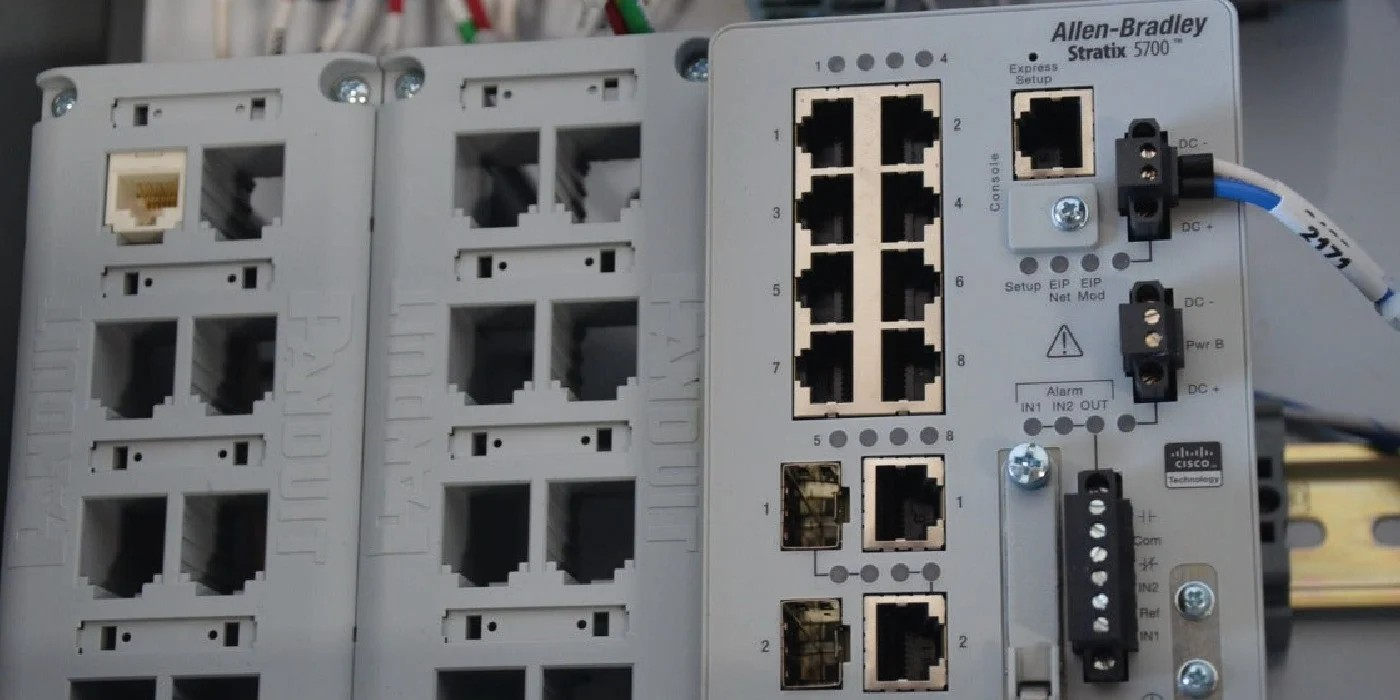
\includegraphics{Img/ethernet.png}

}

\caption{Redes}

\end{figure}%

\begin{enumerate}
\def\labelenumi{\arabic{enumi}.}
\setcounter{enumi}{1}
\tightlist
\item
  \textbf{PLCs y Control de Procesos:}

  \begin{itemize}
  \tightlist
  \item
    Los PLCs han sido una parte integral de la automatización industrial
    durante décadas, y su rol ha evolucionado con la llegada de la
    Industria 4.0. Ahora, los PLCs no solo controlan máquinas
    individuales, sino que también se integran con sistemas más grandes,
    como los ERPs y los sistemas de IoT, para proporcionar un control
    más sofisticado y en tiempo real de los procesos de producción.
  \item
    Los PLCs modernos son capaces de manejar una enorme cantidad de
    datos y realizar cálculos complejos, lo que permite un control más
    preciso y eficiente de los procesos de producción. Además, su
    capacidad de conectarse a redes industriales y compartir datos con
    otros sistemas hace que sean un componente esencial en la
    infraestructura de la Industria 4.0.
  \end{itemize}
\end{enumerate}

\begin{figure}[H]

{\centering 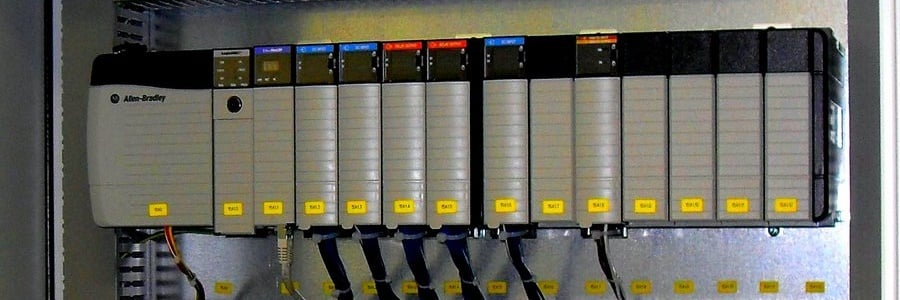
\includegraphics{Img/plc.jpg}

}

\caption{PLC}

\end{figure}%

\begin{enumerate}
\def\labelenumi{\arabic{enumi}.}
\setcounter{enumi}{2}
\tightlist
\item
  \textbf{Sistemas SCADA (Supervisión, Control y Adquisición de Datos):}

  \begin{itemize}
  \tightlist
  \item
    Los sistemas SCADA juegan un papel crucial en la supervisión y
    control de los procesos industriales. En la Industria 4.0, los
    sistemas SCADA se integran con IoT y analítica de datos para
    proporcionar una visión completa y en tiempo real de las
    operaciones, permitiendo a los operadores y gerentes tomar
    decisiones rápidas basadas en datos precisos.
  \item
    Estos sistemas permiten monitorizar en tiempo real las variables
    críticas del proceso, como la temperatura, presión, velocidad de las
    máquinas, etc., y ajustarlas automáticamente para mantener la
    eficiencia y la calidad.
  \end{itemize}
\end{enumerate}

\begin{figure}[H]

{\centering 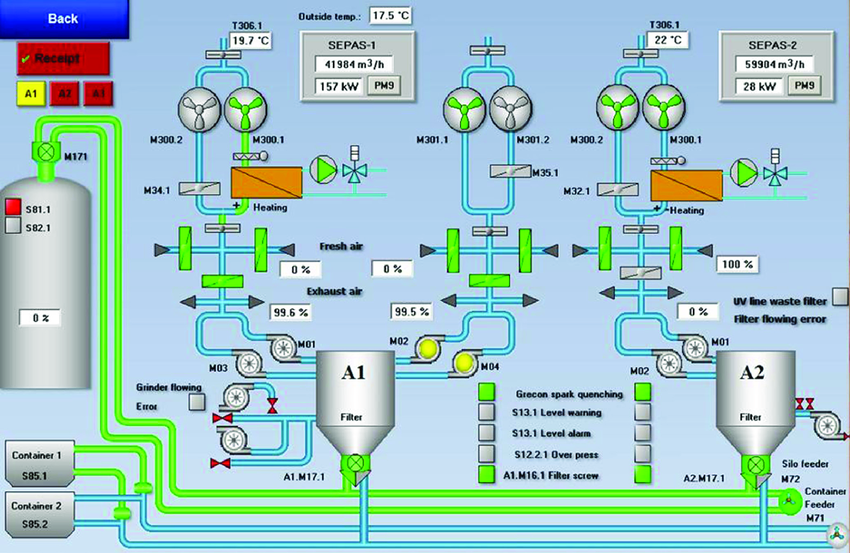
\includegraphics{Img/scada.png}

}

\caption{SCADA}

\end{figure}%

\subsection{La Expansión de los Sistemas
Empresariales}\label{la-expansiuxf3n-de-los-sistemas-empresariales}

La Industria 4.0 también ha impulsado la expansión de los sistemas más
allá de la gestión de recursos empresariales (ERP). Con la creciente
necesidad de integración y eficiencia, las empresas maquiladoras han
comenzado a adoptar una variedad de sistemas especializados que
complementan y amplían las capacidades del ERP tradicional:

\begin{enumerate}
\def\labelenumi{\arabic{enumi}.}
\tightlist
\item
  \textbf{Sistemas de Gestión de la Cadena de Suministro (SCM):}

  \begin{itemize}
  \tightlist
  \item
    Los sistemas SCM se han vuelto críticos en la Industria 4.0, donde
    la sincronización y la coordinación de la cadena de suministro son
    fundamentales. Estos sistemas permiten a las maquilas gestionar de
    manera más eficiente sus relaciones con proveedores, optimizar los
    inventarios y asegurar que los materiales lleguen justo a tiempo
    para la producción.
  \item
    Con la integración de tecnologías IoT y analítica de datos, los
    sistemas SCM pueden proporcionar visibilidad en tiempo real de toda
    la cadena de suministro, permitiendo a las empresas anticiparse a
    problemas antes de que ocurran y ajustar sus operaciones para evitar
    interrupciones.
  \end{itemize}
\item
  \textbf{Sistemas de Gestión de la Relación con el Cliente (CRM):}

  \begin{itemize}
  \tightlist
  \item
    Los sistemas CRM también han evolucionado con la Industria 4.0,
    integrando datos de diferentes fuentes para ofrecer una visión más
    completa del cliente. Esto permite a las maquilas personalizar sus
    productos y servicios de acuerdo con las necesidades del cliente,
    mejorando la satisfacción y fidelización.
  \item
    Con la ayuda de la IA y la analítica avanzada, los sistemas CRM
    pueden predecir las necesidades del cliente antes de que se
    expresen, lo que permite a las empresas adelantarse a la competencia
    y ofrecer soluciones más rápidas y efectivas.
  \end{itemize}
\item
  \textbf{Sistemas de Gestión del Ciclo de Vida del Producto (PLM):}

  \begin{itemize}
  \tightlist
  \item
    Los sistemas PLM gestionan todo el ciclo de vida de un producto,
    desde su diseño inicial hasta su retiro del mercado. En la Industria
    4.0, los PLM se integran con otros sistemas para permitir un
    desarrollo más rápido y eficiente de productos, facilitando la
    colaboración entre departamentos y mejorando la gestión del
    conocimiento.
  \item
    Estos sistemas permiten a las empresas maquiladoras mantener un
    seguimiento de todas las versiones y modificaciones de un producto a
    lo largo de su ciclo de vida, asegurando que la información esté
    siempre actualizada y accesible.
  \end{itemize}
\end{enumerate}

\subsection{Retos y Oportunidades en la Industria
4.0}\label{retos-y-oportunidades-en-la-industria-4.0}

La adopción de la Industria 4.0 trae consigo tanto retos como
oportunidades para las maquilas de Ciudad Juárez. Por un lado, la
inversión en nuevas tecnologías y la reestructuración de los procesos
internos pueden ser costosos y complejos. La necesidad de formación
continua y la integración de múltiples sistemas también pueden
representar desafíos significativos.

Sin embargo, las oportunidades que ofrece la Industria 4.0 son
igualmente grandes. La capacidad de mejorar la eficiencia, reducir
costos, y ofrecer productos personalizados en menos tiempo proporciona
una ventaja competitiva significativa. Además, la integración de
sistemas y la capacidad de tomar decisiones basadas en datos en tiempo
real permiten a las empresas responder más rápidamente a las demandas
del mercado y adaptarse a los cambios de manera más efectiva.

En resumen, la llegada de la Industria 4.0 ha llevado a la industria
maquiladora de Ciudad Juárez a un nuevo nivel de

sofisticación y eficiencia. Las empresas que logren integrar con éxito
estas tecnologías y sistemas estarán mejor posicionadas para prosperar
en un entorno global cada vez más competitivo. La clave está en la
capacidad de adaptarse, innovar y aprovechar al máximo las oportunidades
que ofrece esta nueva era industrial.

\section{Los Grandes Problemas de la Industria
4.0}\label{los-grandes-problemas-de-la-industria-4.0}

La llegada de la Industria 4.0 ha traído consigo una revolución
tecnológica que ha cambiado la manera en que operan las maquilas en
Ciudad Juárez. Sin embargo, esta revolución no ha llegado sin sus
propios desafíos. A medida que las empresas intentan mantenerse al día
con la digitalización y la automatización, se enfrentan a problemas que
pueden frenar su progreso. Entre los más críticos están el manejo del
Big Data, la ciberseguridad, el uso de software privativo que restringe
el acceso y uso de datos, y la gran falta de generación de talento
especializado. Además, comparándonos con otras potencias industriales
como China, nuestro atraso en adoptar completamente la Industria 4.0 se
hace evidente, lo que nos deja en una situación vulnerable frente a la
competencia global.

\subsubsection{Big Data: Un Gigante Difícil de
Domar}\label{big-data-un-gigante-difuxedcil-de-domar}

El Big Data es uno de los aspectos más comentados de la Industria 4.0.
En teoría, tener acceso a grandes volúmenes de datos debería permitir a
las maquilas optimizar sus operaciones, predecir problemas antes de que
ocurran, y tomar decisiones más informadas. Sin embargo, en la práctica,
el manejo de Big Data se ha convertido en un verdadero desafío para
muchas empresas en Ciudad Juárez.

\begin{figure}[H]

{\centering 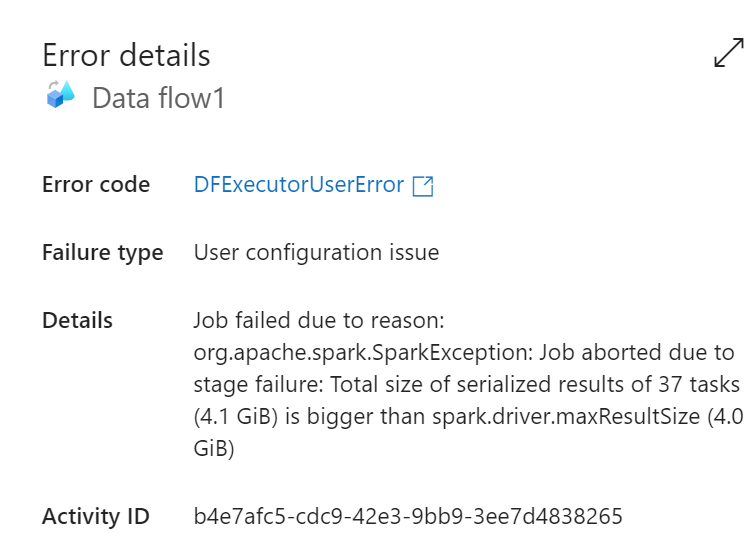
\includegraphics{Img/big.png}

}

\caption{Big Data}

\end{figure}%

\paragraph{Ejemplos de Programas de Big
Data}\label{ejemplos-de-programas-de-big-data}

Uno de los programas más utilizados para manejar Big Data es
\textbf{Apache Hadoop}, una plataforma de código abierto que permite el
procesamiento distribuido de grandes conjuntos de datos a través de
clústeres de computadoras. Hadoop es poderoso, pero requiere una
infraestructura robusta y personal altamente capacitado para su
operación efectiva.

Otro programa clave en el mundo del Big Data es \textbf{Apache Spark},
que se destaca por su velocidad y su capacidad para procesar datos en
tiempo real. Sin embargo, al igual que Hadoop, Spark requiere de una
infraestructura y un equipo de TI que sepa cómo manejarlo, lo que puede
ser un obstáculo para las maquilas que no cuentan con los recursos
necesarios.

\textbf{Tableau} y \textbf{Power BI} son herramientas de visualización
de datos que, aunque no manejan Big Data directamente, permiten a las
empresas interpretar y presentar sus datos de manera más accesible. Sin
embargo, estas herramientas solo son tan buenas como la calidad de los
datos que reciben, lo que significa que, sin una estrategia sólida de
Big Data, su utilidad es limitada.

\begin{figure}[H]

{\centering 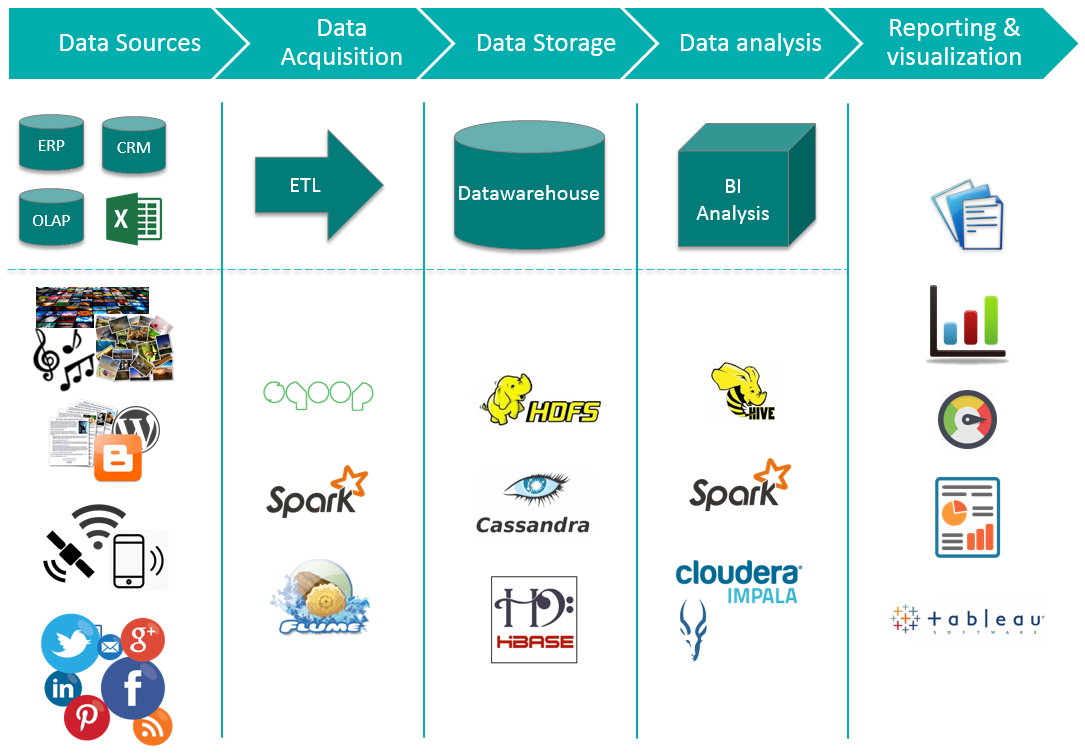
\includegraphics{Img/data.png}

}

\caption{data}

\end{figure}%

\paragraph{Desafíos en el Manejo de Big
Data}\label{desafuxedos-en-el-manejo-de-big-data}

Uno de los principales problemas con Big Data es que muchas maquilas
carecen de la infraestructura adecuada para manejar estos volúmenes
masivos de información. Necesitan servidores potentes, almacenamiento de
datos seguro, y redes rápidas para manejar la transferencia de datos.
Esta infraestructura es costosa y requiere mantenimiento constante, lo
que supone una barrera significativa para las empresas más pequeñas.

Además, el procesamiento y análisis de Big Data requieren personal
altamente capacitado. Los científicos de datos, ingenieros de datos, y
analistas son esenciales para extraer valor de estos datos, pero
encontrar y retener este talento es un reto en sí mismo. A menudo, las
maquilas que intentan implementar estrategias de Big Data se encuentran
con que carecen de los recursos humanos necesarios, lo que lleva a una
subutilización de las herramientas y tecnologías disponibles.

Mientras tanto, en otros países, especialmente en China, el manejo de
Big Data ha sido un foco de inversión masiva. Las empresas chinas han
desarrollado capacidades avanzadas para procesar y analizar grandes
volúmenes de datos, lo que les permite optimizar sus operaciones de
manera que las maquilas de Juárez simplemente no pueden igualar. Esta
brecha tecnológica es preocupante, ya que significa que nuestras
empresas podrían quedarse atrás en un mercado global que cada vez
depende más de la capacidad para manejar y aprovechar los datos.

\subsubsection{Seguridad en la Industria 4.0: Un Riesgo
Constante}\label{seguridad-en-la-industria-4.0-un-riesgo-constante}

La conectividad que trajo la Industria 4.0 ha mejorado mucho la manera
en que trabajamos, pero también ha traído consigo una serie de riesgos
que antes ni imaginábamos. Hoy en día, las maquilas en Juárez están más
expuestas que nunca a ataques cibernéticos. Con todos los sistemas
conectados, desde las máquinas hasta el ERP, cualquier fallo de
seguridad en un punto puede poner en peligro toda la operación.

\paragraph{Ejemplos de Programas de
Seguridad}\label{ejemplos-de-programas-de-seguridad}

En el ámbito de la ciberseguridad, \textbf{Splunk} es uno de los
programas más utilizados para monitorear la seguridad en tiempo real.
Splunk analiza grandes volúmenes de datos y puede detectar
comportamientos anómalos que podrían indicar un ciberataque. Sin
embargo, su implementación y mantenimiento requieren personal capacitado
y una inversión significativa.

\textbf{FireEye} es otra herramienta clave en ciberseguridad, que
proporciona soluciones de detección de amenazas y respuesta rápida ante
incidentes de seguridad. FireEye es potente, pero también caro, lo que
puede ponerlo fuera del alcance de muchas maquilas más pequeñas.

Por otro lado, \textbf{Cisco Umbrella} ofrece seguridad en la nube,
protegiendo a las empresas contra amenazas basadas en internet, como el
phishing y el malware. Aunque es una solución más accesible, también
requiere de una integración adecuada con los sistemas existentes, lo que
puede ser complicado sin el soporte técnico necesario.

\begin{figure}[H]

{\centering 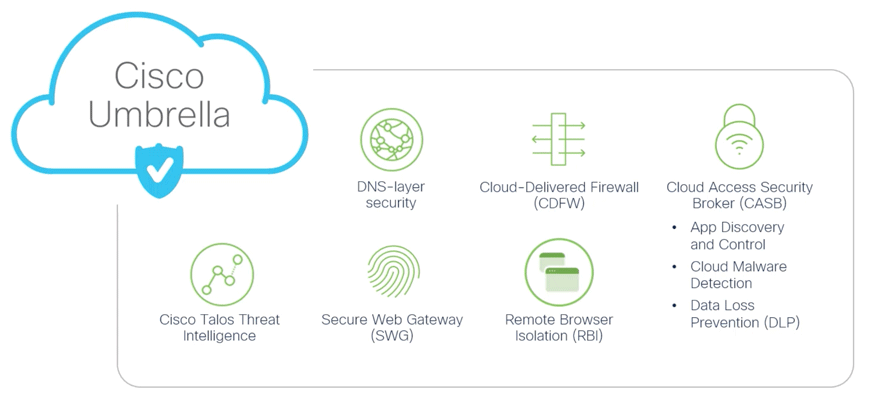
\includegraphics{Img/cisco.png}

}

\caption{umbrella}

\end{figure}%

\paragraph{Desafíos en la
Ciberseguridad}\label{desafuxedos-en-la-ciberseguridad}

Uno de los mayores desafíos en ciberseguridad es mantenerse al día con
las amenazas en constante evolución. Los ciberataques se están volviendo
más sofisticados y frecuentes, y cualquier brecha de seguridad puede
tener consecuencias desastrosas. Para protegerse, las maquilas necesitan
invertir en tecnologías avanzadas y en la formación continua de su
personal, pero esto representa un costo significativo.

Además, la interconexión de todos los sistemas significa que una falla
en un área puede comprometer toda la red. Esto obliga a las empresas a
adoptar un enfoque de seguridad integral, que abarque desde el hardware
hasta el software y los protocolos de usuario. Sin embargo, muchas
maquilas carecen de una estrategia de ciberseguridad bien definida, lo
que las deja vulnerables a ataques que podrían haberse prevenido con
medidas más proactivas.

Mientras tanto, en otras industrias, la ciberseguridad es una prioridad
máxima. En países como China, se han establecido normas estrictas y se
ha invertido mucho en la formación de expertos en seguridad, lo que les
ha permitido proteger mejor sus infraestructuras críticas. Esta
diferencia en el enfoque hacia la ciberseguridad es otro factor que
contribuye a que las maquilas de Juárez se queden atrás en la carrera
por la competitividad global.

\subsubsection{Software Privativo: Un Obstáculo
Inesperado}\label{software-privativo-un-obstuxe1culo-inesperado}

El uso de software privativo es otro de los grandes problemas que
enfrentan las maquilas en la era de la Industria 4.0. Estos sistemas,
aunque poderosos, a menudo imponen restricciones que limitan la
flexibilidad y el control que las empresas tienen sobre sus propios
datos.

\paragraph{Ejemplos de Software
Privativo}\label{ejemplos-de-software-privativo}

\textbf{SAP} es uno de los sistemas ERP más utilizados en la industria
maquiladora, pero es también uno de los más restrictivos en términos de
acceso a los datos. SAP ofrece una gran cantidad de funcionalidades,
pero muchas de ellas están encerradas dentro de su propio ecosistema, lo
que dificulta la integración con otros sistemas o el uso de datos fuera
de su entorno controlado.

\textbf{Oracle} también ofrece soluciones empresariales robustas, pero
al igual que SAP, su enfoque en el software privativo puede limitar la
capacidad de las empresas para utilizar y analizar sus datos de manera
independiente. Las licencias de Oracle son caras, y el software está
diseñado para trabajar dentro de su propio ecosistema, lo que puede ser
una limitación importante para las maquilas que buscan mayor
flexibilidad.

\textbf{Microsoft Dynamics} es otra opción popular, pero también es un
sistema cerrado que impone ciertas restricciones sobre cómo se pueden
utilizar los datos. Aunque Microsoft ofrece una integración más amigable
con otros productos de su suite, sigue siendo un entorno controlado que
puede no ofrecer la libertad que algunas empresas necesitan.

\paragraph{Desafíos del Software
Privativo}\label{desafuxedos-del-software-privativo}

El problema con el software privativo es que, aunque ofrece poderosas
herramientas, también te amarra de manos. Las maquilas que dependen de
estos sistemas se encuentran en una situación en la que no pueden
utilizar sus propios datos fuera del entorno del software, lo que limita
su capacidad para innovar o adaptarse rápidamente a cambios en el
mercado.

Además, la dependencia de un solo proveedor significa que las empresas
están a merced de las decisiones de ese proveedor. Si SAP, Oracle, o
Microsoft deciden cambiar su modelo de negocio, aumentar precios, o
descontinuar soporte para ciertas versiones, las maquilas se encuentran
en una posición difícil, obligadas a seguir la dirección del proveedor o
enfrentarse a costosos procesos de migración.

Esto es particularmente problemático en un entorno de rápida evolución
como la Industria 4.0, donde la flexibilidad y la capacidad de
adaptación son clave para mantenerse competitivo. En contraste, muchas
empresas en China y otros países están adoptando soluciones de código
abierto o desarrollando sus propios sistemas, lo que les da un control
mucho mayor sobre sus datos y procesos. Este enfoque les permite innovar
más rápidamente y adaptarse a los cambios del mercado sin las
restricciones que imponen los sistemas privativos.

\subsubsection{Falta de Talento: Un Talón de
Aquiles}\label{falta-de-talento-un-taluxf3n-de-aquiles}

Sin embargo, el problema más grande al que se enfrenta la Industria 4.0
en Ciudad Juárez es la falta de talento especializado. Mientras que la
tecnología avanza a pasos agigantados, la formación de personal
capacitado no ha seguido el mismo ritmo. Esto ha creado un vacío que es
difícil de llenar, y que está frenando el progreso de muchas maquilas en
su transición hacia la Industria 4.0.

\paragraph{Desafíos en la Generación de
Talento}\label{desafuxedos-en-la-generaciuxf3n-de-talento}

El desafío principal es que la demanda de talento especializado supera
con creces la oferta. Esto significa que las maquilas tienen que
competir no solo entre sí, sino también con empresas de todo el mundo
por los mismos profesionales capacitados. En muchos casos, esto lleva a
una ``guerra de talentos,'' donde las empresas tienen que ofrecer
salarios más altos y beneficios adicionales para atraer y retener a los
expertos que necesitan.

Además, el sistema educativo local no está produciendo el número
suficiente de graduados con las habilidades necesarias. Las
universidades y centros de formación en Ciudad Juárez están tratando de
ponerse al día, pero la brecha entre lo que se enseña y lo que se
necesita en el campo sigue siendo significativa. Esto deja a las
maquilas en una posición difícil, donde tienen que depender de
consultores externos o invertir mucho tiempo y recursos en la
capacitación interna.

En contraste, países como China han hecho de la formación de talento una
prioridad nacional, con programas educativos robustos y alianzas entre
el gobierno, la industria, y las instituciones educativas. Esto les ha
permitido crear un flujo constante de profesionales capacitados listos
para enfrentar los desafíos de la Industria 4.0, mientras que en Juárez
seguimos luchando para llenar las vacantes críticas.

\subsubsection{Atraso vs.~China y Estancamiento en la
Manufactura}\label{atraso-vs.-china-y-estancamiento-en-la-manufactura}

Uno de los efectos más preocupantes de estos desafíos es cómo nos
estamos quedando atrás frente a otras potencias industriales,
especialmente China. Mientras que ellos han integrado la Industria 4.0
en prácticamente todos los aspectos de su economía, nosotros seguimos
rezagados, atrapados en un modelo de maquila tradicional que no termina
de dar el salto hacia la innovación y la creación de valor.

En China, la Industria 4.0 no es solo una tendencia, es una estrategia
de desarrollo nacional. Han invertido millones en tecnología, educación,
y creación de empresas que van mucho más allá de la simple manufactura.
Ellos están liderando en áreas como la inteligencia artificial y la
automatización avanzada, mientras que nosotros seguimos produciendo para
otros, sin desarrollar nuestras propias capacidades tecnológicas.

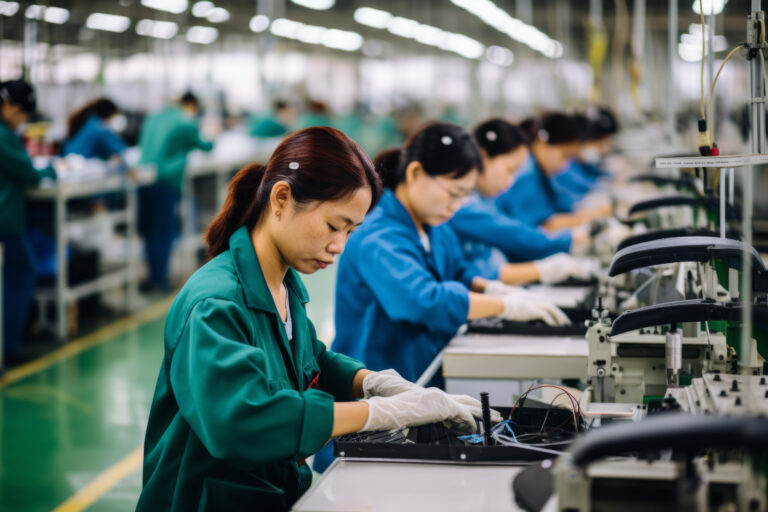
\includegraphics{Img/china.jpg} Este estancamiento nos pone en una
situación vulnerable. Si no tomamos medidas para acelerar la adopción de
la Industria 4.0 y superar estos desafíos, corremos el riesgo de que
nuestras maquilas se queden obsoletas en un mundo que no para de
evolucionar. El desafío es enorme, pero si no lo enfrentamos, podríamos
ver cómo nuestras empresas se quedan atrás, perdiendo competitividad y
relevancia en el mercado global.

\subsection{Reflexión Final}\label{reflexiuxf3n-final}

La Industria 4.0 ofrece una oportunidad increíble para transformar la
industria maquiladora de Ciudad Juárez, pero también nos enfrenta a
retos serios que no podemos ignorar. Si queremos que nuestras empresas
sigan siendo competitivas, necesitamos tomar medidas para superar estos
problemas: mejorar el manejo del Big Data, fortalecer la seguridad,
liberarnos de las limitaciones del software privativo, y, sobre todo,
invertir en la generación de talento especializado.

Es un camino complicado, pero necesario. Si logramos enfrentarnos a
estos desafíos, nuestras maquilas no solo sobrevivirán, sino que podrán
prosperar en un futuro donde la tecnología y la innovación son clave
para el éxito. El tiempo de actuar es ahora, antes de que nos quedemos
completamente rezagados en la carrera industrial global.

\section{Guía Completa para la Adopción Progresiva de la
IA}\label{guuxeda-completa-para-la-adopciuxf3n-progresiva-de-la-ia}

Adoptar la Inteligencia Artificial (IA) en la industria maquiladora es
un reto mayúsculo, pero también una oportunidad que no podemos dejar
pasar si queremos que nuestras maquilas en Ciudad Juárez sigan siendo
competitivas y puedan ponerse al tú por tú con las grandes potencias
industriales del mundo, como China. Sí, es cierto que enfrentamos
desafíos bien duros: la falta de talento especializado, problemas de
ciberseguridad, la dependencia de software privativo que nos ata las
manos con nuestros propios datos, y una cierta sensación de rezago al
compararnos con otras industrias. Pero nada de eso es imposible de
superar. Con un plan bien estructurado, paciencia, y sobre todo con un
compromiso de toda la organización, podemos convertir estos retos en
oportunidades.

Aquí te presento una guía completísima para que, paso a paso, puedas
adoptar la IA en tu maquila de manera gradual, efectiva y sostenible. La
idea no es sólo implementar tecnología por implementarla, sino
transformar tu empresa en una maquila inteligente, capaz de competir en
un mercado global cada vez más exigente.

\begin{quote}
``Implementar estas soluciones requiere una inversión significativa,
tanto en tiempo como en recursos. La realidad es que el mundo no se va a
detener, y si tu maquila no toma las medidas necesarias para adaptarse a
la nueva era tecnológica, te vas a quedar atrás. No solo es una cuestión
de mejora continua, sino de supervivencia. Si no inviertes en modernizar
tu infraestructura, en capacitar a tu equipo, y en adoptar tecnologías
avanzadas como la IA, corres el riesgo de que otra empresa, con un
programa de automatización bien implementado, llegue y te coma el
mandado. Esa empresa podría producir el doble, con menos recursos y a un
costo más bajo, dejándote fuera de la jugada. En un mundo donde la
eficiencia y la innovación son clave, no tomar acción es prácticamente
un boleto directo a la irrelevancia. Así que, aunque el costo inicial
puede parecer alto, la verdad es que no invertir en estas soluciones te
costará mucho más en el largo plazo..''

\begin{itemize}
\tightlist
\item
  \href{https://twitter.com/xavierflorex2}{Javier Flores}
\end{itemize}
\end{quote}

\subsection{Paso 1: Diagnóstico Inicial y Definición de
Objetivos}\label{paso-1-diagnuxf3stico-inicial-y-definiciuxf3n-de-objetivos}

\subsubsection{\texorpdfstring{\textbf{Primero lo Primero: ¿Dónde Estás
Parado?}}{Primero lo Primero: ¿Dónde Estás Parado?}}\label{primero-lo-primero-duxf3nde-estuxe1s-parado}

Antes de lanzarte a meterle IA a tu maquila, lo primero es entender bien
tu punto de partida. No puedes mejorar lo que no conoces, así que hay
que empezar por hacer una radiografía completa de tu empresa: -
\textbf{Infraestructura Tecnológica}: Revisa la tecnología con la que
cuentas actualmente. ¿Tus servidores son lo suficientemente robustos?
¿Tus redes pueden manejar el tráfico de datos que viene con la IA? ¿Tu
almacenamiento es seguro y tiene la capacidad suficiente? Si no tienes
estas bases bien asentadas, cualquier intento de implementar IA podría
quedar en nada. - \textbf{Ciberseguridad}: La seguridad es esencial.
Revisa qué tan protegidos están tus sistemas contra ataques
cibernéticos. ¿Tienes firewalls efectivos? ¿Tus datos están cifrados?
¿Cuentas con un sistema de detección de intrusos? Recuerda que, en la
Industria 4.0, la seguridad no es opcional; es una necesidad. -
\textbf{Talento y Capacidades}: Evalúa el nivel de conocimiento y
habilidades de tu equipo actual en temas relacionados con IA, Big Data,
ciberseguridad, y demás. Identifica dónde hay brechas de conocimiento y
qué habilidades necesitas desarrollar en tu equipo para que puedan
manejar y sacar el máximo provecho de estas nuevas tecnologías.

\subsubsection{\texorpdfstring{\textbf{Definir Objetivos Claros y
Alcanzables}}{Definir Objetivos Claros y Alcanzables}}\label{definir-objetivos-claros-y-alcanzables}

Conocer dónde estás es solo el primer paso. Ahora, tienes que definir
adónde quieres llegar: - \textbf{Corto Plazo (1-2 años)}: Aquí es donde
puedes enfocarte en mejoras rápidas y de impacto inmediato. Por ejemplo,
la automatización de tareas repetitivas que actualmente se hacen de
manera manual en la línea de producción. Esto no sólo te ahorra tiempo,
sino que también reduce errores y aumenta la eficiencia. -
\textbf{Mediano Plazo (3-5 años)}: Una vez que las primeras mejoras
estén funcionando bien, puedes pensar en implementar mantenimiento
predictivo con IA. Esto te permitirá anticiparte a los problemas antes
de que ocurran, evitando paros no programados y extendiendo la vida útil
de tus equipos. - \textbf{Largo Plazo (5-10 años)}: Aquí es donde
empiezas a soñar en grande. Piensa en la integración total de la IA en
todas las operaciones de la maquila, desde la optimización de la cadena
de suministro hasta la automatización de la toma de decisiones
estratégicas. La idea es que tu empresa funcione como un todo
coordinado, con cada parte optimizada y alineada para maximizar la
eficiencia y la productividad.

\begin{figure}[H]

{\centering 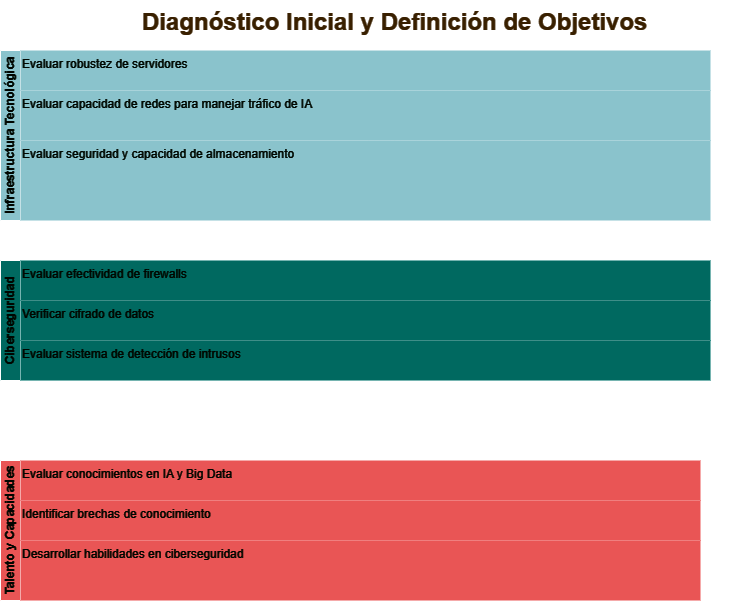
\includegraphics{Img/paso1.png}

}

\caption{Paso 1}

\end{figure}%

\subsection{Paso 2: Mejora la Infraestructura y Desarrolla el
Talento}\label{paso-2-mejora-la-infraestructura-y-desarrolla-el-talento}

\subsubsection{\texorpdfstring{\textbf{Ponte al Día con la
Infraestructura}}{Ponte al Día con la Infraestructura}}\label{ponte-al-duxeda-con-la-infraestructura}

Una vez que tengas claros tus objetivos, es momento de asegurarte de que
tienes la infraestructura necesaria para lograrlos: - \textbf{Actualiza
tus Sistemas}: Si tus servidores ya están viejos o no tienes suficiente
capacidad de almacenamiento, es momento de actualizar. Considera migrar
a soluciones en la nube, como AWS o Google Cloud, que te ofrecen la
escalabilidad y la flexibilidad que necesitas para manejar el incremento
de datos que vendrá con la implementación de IA. - \textbf{Cambia tu
Red}: Si tus redes ya no son eficientes o no tienes suficiente capacidad
de procesamiento, es momento de cambiar. Por ejemplo, puedes mover tus
servidores a una red de datos en la nube. -
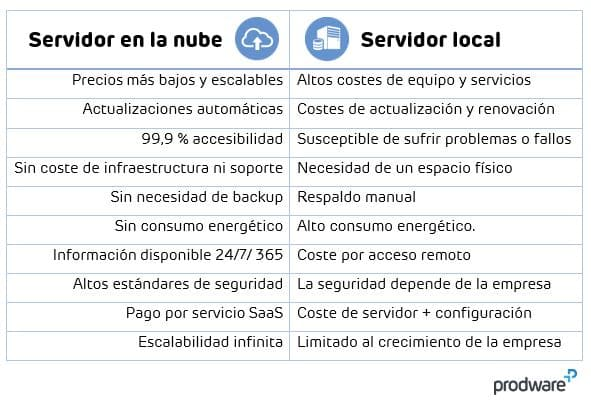
\includegraphics{Img/cloud.jpg}

\begin{itemize}
\tightlist
\item
  \textbf{Fortalece la Seguridad}: La ciberseguridad es una prioridad.
  Invierte en firewalls de última generación, sistemas de detección de
  intrusos, y asegúrate de que todos los datos sensibles estén cifrados
  tanto en tránsito como en reposo. También es vital que establezcas
  protocolos de seguridad claros y que todo tu equipo los entienda y
  cumpla.
\end{itemize}

\subsubsection{\texorpdfstring{\textbf{Capacita a tu Gente: El Talento
es la
Clave}}{Capacita a tu Gente: El Talento es la Clave}}\label{capacita-a-tu-gente-el-talento-es-la-clave}

La tecnología por sí sola no es suficiente; necesitas un equipo
capacitado que sepa cómo manejarla y sacarle el máximo provecho: -
\textbf{Capacitación Interna}: No esperes a que el talento especializado
llegue a tocar tu puerta. Inicia programas de capacitación interna para
que tu equipo actual pueda desarrollar las habilidades necesarias.
Plataformas como \textbf{Coursera}, \textbf{Udemy}, y . \textbf{IA
Center} ofrecen cursos en áreas clave como inteligencia artificial,
análisis de datos, y ciberseguridad. También puedes considerar traer a
expertos para que den talleres o cursos en tu empresa o simplem
networking.

\begin{figure}[H]

{\centering 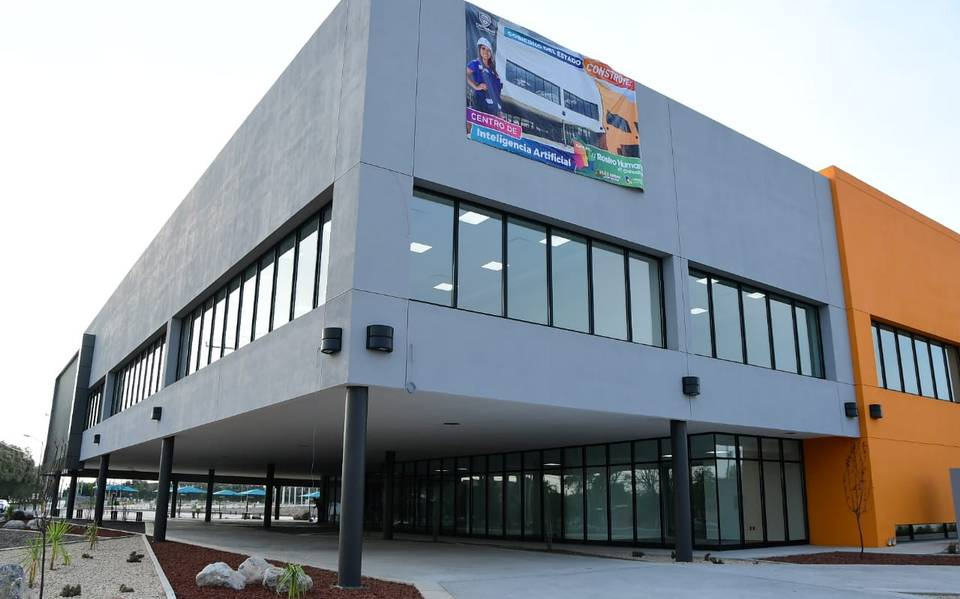
\includegraphics{Img/iacenter.jpeg}

}

\caption{IA Center}

\end{figure}%

\begin{itemize}
\tightlist
\item
  \textbf{Alianzas con Universidades}: Establece relaciones con
  universidades locales y centros de formación técnica para desarrollar
  programas que preparen a los estudiantes específicamente para las
  necesidades de la Industria 4.0 en la maquila. Esto no solo te ayudará
  a formar nuevo talento, sino que también te permitirá atraer a los
  mejores candidatos una vez que estén listos para el mercado laboral.
\end{itemize}

\begin{figure}[H]

{\centering 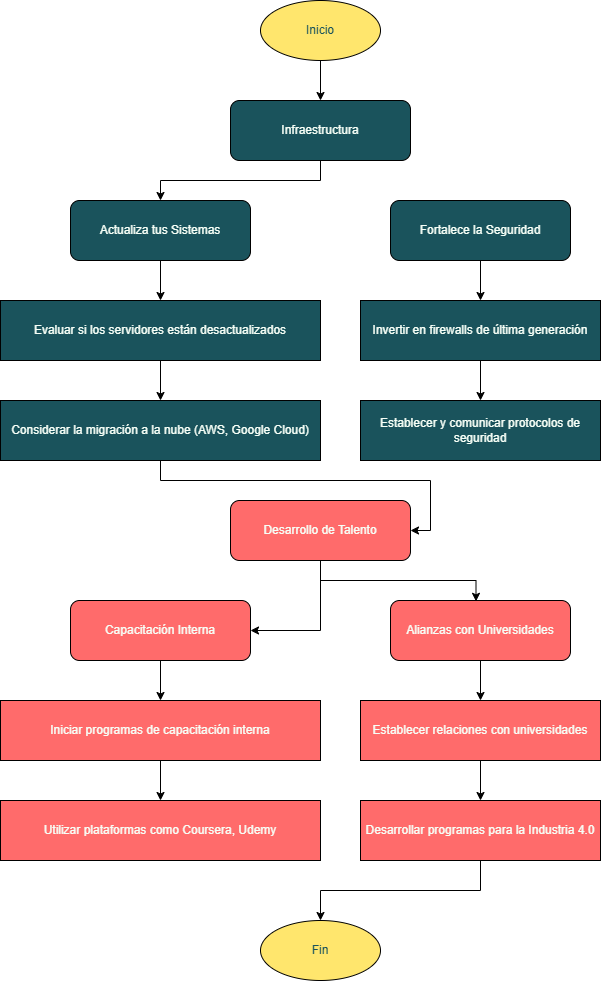
\includegraphics{Img/paso3.png}

}

\caption{Paso 3}

\end{figure}%

\subsection{Paso 3: Implementación Inicial de IA en Áreas
Específicas}\label{paso-3-implementaciuxf3n-inicial-de-ia-en-uxe1reas-especuxedficas}

\subsubsection{\texorpdfstring{\textbf{Paso a Paso: Empieza con
Proyectos
Piloto}}{Paso a Paso: Empieza con Proyectos Piloto}}\label{paso-a-paso-empieza-con-proyectos-piloto}

Transformar toda la maquila de un jalón es como querer correr antes de
aprender a caminar. Es mejor empezar despacio, con proyectos piloto en
áreas clave donde la IA pueda mostrar su valor de manera rápida y clara.
Al hacer esto, no solo reduces el riesgo, sino que también puedes
demostrar a todo el equipo los beneficios tangibles de adoptar esta
tecnología. Aquí te doy algunos ejemplos y recomendaciones para
arrancar:

\begin{itemize}
\item
  \textbf{Selecciona Casos de Uso Específicos}

  Aquí es donde tienes que ponerle coco y pensar en qué partes de tu
  operación necesitan una mejora urgente o dónde la IA puede resolver un
  problema que lleva tiempo molestando. Busca esos puntos críticos donde
  la IA pueda hacer una diferencia real y rápida. Te doy unos ejemplos:

  \begin{itemize}
  \item
    \textbf{Mantenimiento Predictivo}: Imagina poder anticiparte a los
    problemas de tus máquinas antes de que sucedan. Con la IA, puedes
    analizar los datos que generan las máquinas todos los días y
    predecir cuándo es probable que se descompongan. Esto te permite
    hacer el mantenimiento justo a tiempo, antes de que la máquina falle
    por completo, evitando paros inesperados y reduciendo costos de
    reparación. Es como si pudieras ver el futuro y saber cuándo algo va
    a fallar.
  \item
    \textbf{Control de Calidad Automatizado}: Otro gran uso de la IA es
    en el control de calidad. En lugar de revisar manualmente cada
    producto, puedes usar tecnología que inspeccione cada pieza con una
    precisión increíble. Esto no solo acelera el proceso, sino que
    también asegura que todos los productos cumplan con los estándares
    de calidad. Además, reduce el desperdicio porque detecta errores
    antes de que sea demasiado tarde.
  \item
    \textbf{Optimización de Inventarios}: La IA también puede ayudarte a
    manejar mejor tus inventarios. Con herramientas que analizan las
    ventas pasadas y otras variables, puedes predecir cuánto stock
    necesitarás en el futuro, evitando que te quedes corto o que tengas
    exceso de inventario. Así, optimizas tus recursos y ahorras dinero.
  \end{itemize}
\item
  \textbf{Desarrollo de Prototipos de IA}

  No te lances a lo grande sin antes probar las cosas en pequeño.
  Trabaja junto con tu equipo de TI y, si es necesario, colabora con
  expertos externos para desarrollar versiones iniciales (prototipos) de
  las soluciones de IA que quieras implementar. Estos prototipos te
  permiten probar diferentes enfoques sin comprometerte por completo, lo
  que te da la flexibilidad de ajustar y mejorar antes de hacer un
  despliegue más amplio.

  Por ejemplo, si decides probar un sistema de mantenimiento predictivo,
  puedes empezar con una sola máquina o un solo proceso, monitoreando
  cómo se comporta y ajustando la tecnología según sea necesario. Con el
  tiempo, puedes ampliar el uso de la IA a más máquinas o procesos, una
  vez que estés seguro de que todo está funcionando bien.
\end{itemize}

\subsubsection{\texorpdfstring{\textbf{Monitoreo y Ajuste: Perfecciona
sobre la
Marcha}}{Monitoreo y Ajuste: Perfecciona sobre la Marcha}}\label{monitoreo-y-ajuste-perfecciona-sobre-la-marcha}

Implementar IA no es algo que haces una vez y ya está. Necesitas estar
al pendiente de cómo están funcionando los proyectos piloto y hacer
ajustes sobre la marcha para asegurarte de que todo está jalando como
debe:

\begin{itemize}
\item
  \textbf{Pruebas de Rendimiento}

  Después de poner en marcha los proyectos piloto, es esencial que sigas
  de cerca cómo están funcionando. Revisa constantemente si están
  cumpliendo con lo que esperabas: ¿Están reduciendo los costos? ¿Están
  mejorando la eficiencia? ¿Qué tan bien están funcionando las
  predicciones? Estos son los tipos de preguntas que debes hacerte
  mientras monitoreas el rendimiento.

  Si algo no está saliendo como esperabas, no te preocupes; es normal.
  Aquí es donde entra la fase de ajuste. Puede que necesites modificar
  cómo estás usando la IA, cambiar algunos parámetros, o incluso
  reconsiderar el enfoque inicial. Lo importante es que estés dispuesto
  a adaptarte y hacer los cambios necesarios para que los sistemas
  funcionen cada vez mejor.
\item
  \textbf{Retroalimentación Continua}

  No te olvides de hablar con tu equipo. Ellos son los que están usando
  estas nuevas herramientas todos los días y te pueden dar una
  perspectiva valiosa sobre lo que está funcionando y lo que no. Tal vez
  te digan que algunas predicciones no son tan precisas como esperaban,
  o que el sistema es un poco complicado de usar. Escucha sus
  comentarios y usa esa información para hacer ajustes que realmente
  mejoren la operación.

  Hacer esto no solo te ayudará a mejorar la implementación de la IA,
  sino que también hará que tu equipo se sienta involucrado en el
  proceso de cambio, lo que es clave para el éxito a largo plazo.
\end{itemize}

Este paso es crucial porque es donde empiezas a ver los beneficios
reales de la IA, pero también donde te das cuenta de que esto es un
proceso continuo. No se trata solo de instalar la tecnología y esperar
que todo funcione, sino de estar siempre mejorando y ajustando para
obtener los mejores resultados. Si lo haces bien, estos proyectos piloto
se convertirán en la base para una transformación más amplia y profunda
en tu maquila.

\bookmarksetup{startatroot}

\chapter{Aplicaciones de la Inteligencia Artificial en la
Maquiladora}\label{aplicaciones-de-la-inteligencia-artificial-en-la-maquiladora}

\section{El Camino para Adaptar la Inteligencia Artificial en la
Maquiladora}\label{el-camino-para-adaptar-la-inteligencia-artificial-en-la-maquiladora}

La neta es que, hoy en día, la Inteligencia Artificial (IA) ya no es
solo un lujo o una moda; es una necesidad si quieres seguir rifando en
la maquila. En Ciudad Juárez, donde la maquila es el mero corazón
económico, adaptarse a la IA puede hacer la diferencia entre seguir
liderando o quedarte atrás viendo cómo otros te comen el mandado. Pero,
eso sí, hay que ser realistas: meterle IA a la maquila no es tan fácil
como cambiar de máquina o implementar un nuevo software. Es un proceso
que puede ser más o menos complicado, dependiendo de varios factores
como lo técnico, el tiempo que toma, la lana que hay que invertir, y qué
tan listos están tus trabajadores para aceptar el cambio.

Para hacerte la vida más sencilla, hemos desarrollado un \textbf{Ranking
de Adaptación a la IA en la Maquiladora}, que desglosa estos factores
clave para que tengas una mejor idea de qué tan complicado puede ser
para tu maquila subirse al tren de la IA. Con este ranking, podrás
evaluar qué áreas de tu maquila necesitan más atención y qué tanto
esfuerzo te va a costar hacer la transición.

\subsection{Ranking de Adaptación a la
IA}\label{ranking-de-adaptaciuxf3n-a-la-ia}

\begin{enumerate}
\def\labelenumi{\arabic{enumi}.}
\tightlist
\item
  \textbf{Complejidad Técnica}

  \begin{itemize}
  \tightlist
  \item
    \textbf{Alto (5)}: Aquí estamos hablando de cosas que requieren
    conocimientos bien pesados en programación y sistemas complejos.
    Esos proyectos que, si no traes un equipo de TI al cien, te van a
    costar sudor y lágrimas. Ejemplos: Implementar redes neuronales
    profundas para análisis en tiempo real o desarrollar sistemas de
    mantenimiento predictivo que monitoreen un chorro de datos.
  \item
    \textbf{Medio (3)}: Proyectos que ya te piden saberle un poquito a
    la programación, pero que no son una misión imposible. Son cosas que
    implican conectar lo que ya tienes con software de IA, tal vez con
    una que otra personalización. Ejemplos: Usar software de visión por
    computadora para revisar la calidad o meterle chatbots para atender
    a los clientes.
  \item
    \textbf{Bajo (1)}: Aquí estamos hablando de soluciones casi listas
    para usarse, que no te piden saber de códigos ni meterte en broncas
    técnicas. Ejemplos: Plataformas de análisis de datos con IA ya
    configurada o herramientas que te automatizan tareas sencillas.
  \end{itemize}
\item
  \textbf{Tiempo de Implementación}

  \begin{itemize}
  \tightlist
  \item
    \textbf{Largo (5)}: Proyectos que, la neta, van a tomar más de un
    año para completarse. Son esos que necesitan mucho desarrollo a la
    medida, pruebas y que además te piden capacitar a tu gente a fondo.
    Ejemplos: Crear un sistema de IA para manejar toda la cadena de
    suministro.
  \item
    \textbf{Medio (3)}: Implementaciones que te van a tomar entre seis
    meses y un año. No son rápidas, pero tampoco eternas. Ejemplos:
    Meter IA para optimizar inventarios o mejorar la logística interna.
  \item
    \textbf{Corto (1)}: Proyectos que, si le metes ganas, puedes
    terminar en menos de seis meses. Ejemplos: Automatizar tareas
    administrativas o usar IA para predecir ventas.
  \end{itemize}
\item
  \textbf{Inversión Económica}

  \begin{itemize}
  \tightlist
  \item
    \textbf{Alta (5)}: Aquí ya estamos hablando de desembolsar una lana
    considerable. No solo en tecnología, sino también en infraestructura
    y capacitar a tu banda. Ejemplos: Implementar IA en varias áreas de
    producción o comprar robots industriales avanzados con IA.
  \item
    \textbf{Media (3)}: Inversiones más accesibles, donde la lana se
    reparte entre tecnología y capacitación, sin volverte loco.
    Ejemplos: Meter sistemas de mantenimiento predictivo o mejorar el
    control de calidad con visión por computadora.
  \item
    \textbf{Baja (1)}: Proyectos que no te van a dejar en números rojos.
    Tecnología accesible y poca necesidad de cambios grandes. Ejemplos:
    Usar plataformas de análisis de datos con IA o meter asistentes
    virtuales para tareas sencillas.
  \end{itemize}
\item
  \textbf{Capacitación y Adaptación del Personal}

  \begin{itemize}
  \tightlist
  \item
    \textbf{Alta (5)}: Si decides entrarle a algo que requiere un cambio
    radical, prepárate para invertir tiempo y esfuerzo en capacitar a tu
    gente. Aquí la curva de aprendizaje es empinada. Ejemplos: Formar a
    tu equipo en desarrollo de IA, análisis de datos, y gestión de
    proyectos grandes.
  \item
    \textbf{Media (3)}: Capacitación moderada, pero necesaria. Aquí tu
    gente tiene que aprender a usar nuevas herramientas y entender lo
    básico de la IA. Ejemplos: Entrenar al personal en el uso de
    software de control de calidad automatizado o manejar inventarios
    con IA.
  \item
    \textbf{Baja (1)}: Proyectos que no te van a pedir casi nada en
    términos de capacitación. Herramientas fáciles de usar que no
    cambian mucho la forma en que tu banda trabaja. Ejemplos:
    Implementar herramientas de análisis de datos con interfaces
    sencillas o usar chatbots ya preconfigurados.
  \end{itemize}
\item
  \textbf{Impacto en la Cultura Organizacional}

  \begin{itemize}
  \tightlist
  \item
    \textbf{Alto (5)}: Aquí estás hablando de un cambio de raíz en la
    manera de trabajar y gestionar la producción. Es un cambio profundo
    que va a impactar a toda la maquila. Ejemplos: Una transformación
    digital completa que integre IA en todos los niveles de la maquila.
  \item
    \textbf{Medio (3)}: Requiere ajustes en la forma de trabajar, pero
    no cambia la cultura de arriba abajo. Ejemplos: Automatizar procesos
    específicos sin cambiar todo el flujo de trabajo.
  \item
    \textbf{Bajo (1)}: Cambios que tienen un impacto mínimo en la
    cultura de la maquila. Se integran fácilmente en la rutina diaria
    sin mayores broncas. Ejemplos: Usar IA en tareas administrativas o
    para mejoras puntuales en áreas no críticas.
  \end{itemize}
\end{enumerate}

\subsection{Reflexión Final}\label{reflexiuxf3n-final-1}

Este ranking te da un panorama claro de los retos y requisitos que
vienen con la adaptación de la IA en tu maquila. No todas las empresas
están en el mismo punto, y no todas tienen que seguir el mismo camino.
Lo importante es saber dónde estás parado y planificar la transición
para que le saques el máximo jugo a la IA mientras minimizas los
riesgos.

Adoptar la IA no es solo subirse a la ola tecnológica; es una necesidad
para seguir siendo competitivos en un mundo donde la eficiencia, la
precisión, y la capacidad de adaptarse rápido son la clave del éxito. El
camino hacia la IA será diferente para cada maquila, pero con una buena
planificación y una implementación gradual, todas pueden aprovechar los
beneficios que esta tecnología ofrece. ¡Así que a darle con todo,
Juárez!

\section{Aplicaciones de la Inteligencia Artificial en la
Maquiladora}\label{aplicaciones-de-la-inteligencia-artificial-en-la-maquiladora-1}

\section{Machine Learning
Tradicional}\label{machine-learning-tradicional}

La Inteligencia Artificial (IA) ha llegado para cambiar el juego en la
industria maquiladora. Desde la optimización de procesos hasta la
gestión de la cadena de suministro, la IA ofrece un sinfín de
posibilidades para mejorar la eficiencia, reducir costos y elevar la
calidad de los productos. Sin embargo, la implementación de estas
tecnologías puede variar significativamente en términos de complejidad
técnica, tiempo de implementación, inversión necesaria y el impacto en
la cultura organizacional.

En este capítulo, vamos a explorar más a fondo cómo la IA puede ser
aplicada en la maquiladora, desglosando cada área con mayor detalle y
proporcionando un listado de tecnologías clave que pueden ser utilizadas
en cada caso.

\subsection{Proyecto 1. Optimización del Proceso de
Producción}\label{proyecto-1.-optimizaciuxf3n-del-proceso-de-producciuxf3n}

\textbf{Ranking de Adaptación:}

\begin{longtable}[]{@{}ll@{}}
\toprule\noalign{}
Factor & Valor \\
\midrule\noalign{}
\endhead
\bottomrule\noalign{}
\endlastfoot
Complejidad Técnica & Alto (5) \\
Tiempo de Implementación & Medio (3) \\
Inversión Económica & Alta (5) \\
Capacitación del Personal & Media (3) \\
Impacto en la Cultura Organizacional & Alto (5) \\
\end{longtable}

\textbf{Aplicaciones:}

\textbf{a. Mantenimiento Predictivo:}

El mantenimiento predictivo es una aplicación clave de la IA en la
industria maquiladora. Permite monitorear el estado de las máquinas en
tiempo real y predecir fallas antes de que ocurran, lo que se traduce
en:

\begin{itemize}
\tightlist
\item
  \textbf{Reducción de tiempos de inactividad no planificados:} Evitar
  paradas inesperadas de la producción aumenta la eficiencia y la
  productividad.
\item
  \textbf{Optimización de los costos de mantenimiento:} Al realizar el
  mantenimiento solo cuando es necesario, se ahorra en costos de
  repuestos y mano de obra.
\item
  \textbf{Extensión de la vida útil de los equipos:} Detectar y
  solucionar problemas a tiempo contribuye a prolongar la vida útil de
  la maquinaria.
\end{itemize}

\textbf{Tecnologías Clave:}

\begin{itemize}
\tightlist
\item
  \textbf{Sensores IoT (Internet of Things):} Estos dispositivos
  recopilan datos vitales sobre el funcionamiento de las máquinas, como
  vibración, temperatura, presión, etc.
\item
  \textbf{Plataformas de Machine Learning:} Herramientas como
  TensorFlow, PyTorch o Azure Machine Learning procesan los datos de los
  sensores y construyen modelos predictivos que identifican patrones y
  anomalías.
\item
  \textbf{Software de Mantenimiento Predictivo:} Soluciones
  especializadas como IBM Maximo o GE Predix integran la IA para
  analizar los datos en tiempo real, generar alertas tempranas y
  programar el mantenimiento de manera proactiva.
\end{itemize}

\textbf{Tabla Resumen:}

\begin{longtable}[]{@{}
  >{\raggedright\arraybackslash}p{(\columnwidth - 4\tabcolsep) * \real{0.3333}}
  >{\raggedright\arraybackslash}p{(\columnwidth - 4\tabcolsep) * \real{0.3333}}
  >{\raggedright\arraybackslash}p{(\columnwidth - 4\tabcolsep) * \real{0.3333}}@{}}
\toprule\noalign{}
\begin{minipage}[b]{\linewidth}\raggedright
Aplicación
\end{minipage} & \begin{minipage}[b]{\linewidth}\raggedright
Beneficios
\end{minipage} & \begin{minipage}[b]{\linewidth}\raggedright
Tecnologías Clave
\end{minipage} \\
\midrule\noalign{}
\endhead
\bottomrule\noalign{}
\endlastfoot
Mantenimiento Predictivo & Reducción de tiempos de inactividad,
optimización de costos de mantenimiento, extensión de la vida útil de
los equipos & Sensores IoT, plataformas de Machine Learning, software de
Mantenimiento Predictivo \\
\end{longtable}

\textbf{Consideraciones Adicionales:}

\begin{itemize}
\tightlist
\item
  \textbf{Inversión inicial:} La implementación de un sistema de
  mantenimiento predictivo requiere una inversión significativa en
  sensores, software y capacitación del personal.
\item
  \textbf{Integración con sistemas existentes:} Es importante asegurar
  la compatibilidad y la integración fluida con los sistemas de gestión
  de mantenimiento y producción ya existentes en la empresa.
\item
  \textbf{Cultura de datos:} Fomentar una cultura basada en datos es
  fundamental para aprovechar al máximo el potencial del mantenimiento
  predictivo y la toma de decisiones informadas.
\end{itemize}

\textbf{En resumen:} El mantenimiento predictivo, impulsado por la IA,
ofrece una oportunidad valiosa para las maquiladoras de optimizar sus
procesos de producción, reducir costos y mejorar la eficiencia. A pesar
de la inversión inicial y la complejidad técnica, los beneficios a largo
plazo hacen que esta aplicación sea una consideración estratégica para
cualquier empresa que busque mantenerse competitiva en el mercado
actual.

\textbf{b. Control de Calidad Automatizado:}

El control de calidad es crucial en la maquila, y la IA puede
revolucionar esta área. Con sistemas de visión por computadora y
aprendizaje automático, la IA puede inspeccionar cada producto en la
línea de producción, identificando defectos que serían difíciles de
detectar manualmente.

\begin{itemize}
\tightlist
\item
  \textbf{Tecnologías Clave:}

  \begin{itemize}
  \tightlist
  \item
    \textbf{Cámaras de Visión por Computadora:} Equipos como los de
    \textbf{Cognex} o \textbf{Basler} que capturan imágenes de alta
    resolución de los productos.
  \item
    \textbf{Software de Análisis de Imágenes:} Herramientas como
    \textbf{OpenCV} o \textbf{MATLAB} que procesan las imágenes y
    detectan defectos.
  \item
    \textbf{Redes Neuronales Convolucionales (CNNs):} Algoritmos que
    permiten a la IA reconocer patrones y diferencias sutiles en los
    productos.
  \end{itemize}
\end{itemize}

\textbf{c.~Optimización del Flujo de Trabajo:}

La IA también puede ser utilizada para optimizar el flujo de trabajo en
la maquila. Analizando datos de producción, la IA puede identificar
cuellos de botella y sugerir ajustes en tiempo real para mejorar la
eficiencia.

\begin{itemize}
\tightlist
\item
  \textbf{Tecnologías Clave:}

  \begin{itemize}
  \tightlist
  \item
    \textbf{Sistemas MES (Manufacturing Execution Systems):} Plataformas
    como \textbf{Siemens SIMATIC IT} que integran IA para la gestión del
    flujo de trabajo.
  \item
    \textbf{Análisis de Datos en Tiempo Real:} Herramientas como
    \textbf{Apache Kafka} y \textbf{Elasticsearch} que procesan y
    analizan grandes volúmenes de datos de producción.
  \item
    \textbf{Algoritmos de Optimización:} Uso de técnicas como
    \textbf{Programación Lineal} y \textbf{Algoritmos Genéticos} para
    ajustar el flujo de trabajo y maximizar la eficiencia.
  \end{itemize}
\end{itemize}

\subsection{Proyecto 2. Gestión de la Cadena de
Suministro}\label{proyecto-2.-gestiuxf3n-de-la-cadena-de-suministro}

\textbf{Ranking de Adaptación:}

\begin{longtable}[]{@{}ll@{}}
\toprule\noalign{}
Factor & Valor \\
\midrule\noalign{}
\endhead
\bottomrule\noalign{}
\endlastfoot
Complejidad Técnica & Medio (3) \\
Tiempo de Implementación & Medio (3) \\
Inversión Económica & Media (3) \\
Capacitación del Personal & Baja (1) \\
Impacto en la Cultura Organizacional & Medio (3) \\
\end{longtable}

\textbf{Aplicaciones:}

\textbf{a. Optimización de Inventarios:}

La gestión eficiente de inventarios es crucial en la industria
maquiladora. La IA permite predecir la demanda futura con mayor
precisión, lo que ayuda a evitar tanto el exceso de stock (que genera
costos de almacenamiento) como la falta de stock (que puede provocar
interrupciones en la producción).

\textbf{Beneficios:}

\begin{itemize}
\tightlist
\item
  Reducción de costos de almacenamiento
\item
  Mejora de la disponibilidad de productos
\item
  Mayor eficiencia en la cadena de suministro
\end{itemize}

\textbf{Tecnologías Clave:}

\begin{itemize}
\tightlist
\item
  \textbf{Algoritmos de Predicción:} Utilizan datos históricos para
  pronosticar la demanda futura. Ejemplos incluyen Regresión Lineal y
  Redes Neuronales Recurrentes (RNNs).
\item
  \textbf{Plataformas de Gestión de Inventarios:} Integran las
  predicciones de IA para optimizar los niveles de inventario.
\item
  \textbf{Sensores IoT para Inventarios:} Monitorean los niveles de
  stock en tiempo real para una gestión más precisa.
\end{itemize}

\textbf{b. Logística Inteligente:}

La IA puede mejorar significativamente la eficiencia de la logística en
la maquila. Los algoritmos de optimización permiten seleccionar las
rutas de transporte más eficientes, programar envíos de manera óptima y
realizar ajustes en tiempo real a las operaciones logísticas.

\textbf{Beneficios:}

\begin{itemize}
\tightlist
\item
  Reducción de costos de transporte
\item
  Mejora de los tiempos de entrega
\item
  Mayor agilidad y capacidad de respuesta en la logística
\end{itemize}

\textbf{Tecnologías Clave:}

\begin{itemize}
\tightlist
\item
  \textbf{Algoritmos de Optimización de Rutas:} Encuentran las rutas más
  rápidas y económicas para el transporte de mercancías.
\item
  \textbf{Sistemas de Gestión de Transporte (TMS):} Utilizan IA para
  optimizar la planificación y ejecución del transporte.
\item
  \textbf{Plataformas de Análisis Predictivo:} Analizan datos históricos
  y en tiempo real para anticipar problemas y optimizar las operaciones
  logísticas.
\end{itemize}

\textbf{Tabla Resumen}

\begin{longtable}[]{@{}
  >{\raggedright\arraybackslash}p{(\columnwidth - 4\tabcolsep) * \real{0.3333}}
  >{\raggedright\arraybackslash}p{(\columnwidth - 4\tabcolsep) * \real{0.3333}}
  >{\raggedright\arraybackslash}p{(\columnwidth - 4\tabcolsep) * \real{0.3333}}@{}}
\toprule\noalign{}
\begin{minipage}[b]{\linewidth}\raggedright
Aplicación
\end{minipage} & \begin{minipage}[b]{\linewidth}\raggedright
Beneficios
\end{minipage} & \begin{minipage}[b]{\linewidth}\raggedright
Tecnologías Clave
\end{minipage} \\
\midrule\noalign{}
\endhead
\bottomrule\noalign{}
\endlastfoot
Optimización de Inventarios & Reducción de costos de almacenamiento,
mejora de la disponibilidad de productos, mayor eficiencia en la cadena
de suministro & Algoritmos de Predicción, Plataformas de Gestión de
Inventarios, Sensores IoT para Inventarios \\
Logística Inteligente & Reducción de costos de transporte, mejora de los
tiempos de entrega, mayor agilidad y capacidad de respuesta en la
logística & Algoritmos de Optimización de Rutas, Sistemas de Gestión de
Transporte (TMS), Plataformas de Análisis Predictivo \\
\end{longtable}

\textbf{En resumen:} La aplicación de la IA en la gestión de la cadena
de suministro ofrece a las maquiladoras la oportunidad de optimizar sus
operaciones, reducir costos y mejorar la eficiencia en áreas clave como
la gestión de inventarios y la logística. La implementación de estas
tecnologías puede requerir cierta inversión y adaptación, pero los
beneficios potenciales son significativos y pueden contribuir a una
mayor competitividad en el mercado.

\subsection{Proyecto 3. Automatización de Tareas
Repetitivas}\label{proyecto-3.-automatizaciuxf3n-de-tareas-repetitivas}

\textbf{Ranking de Adaptación:}

\begin{longtable}[]{@{}ll@{}}
\toprule\noalign{}
Factor & Valor \\
\midrule\noalign{}
\endhead
\bottomrule\noalign{}
\endlastfoot
Complejidad Técnica & Bajo (1) \\
Tiempo de Implementación & Corto (1) \\
Inversión Económica & Baja (1) \\
Capacitación del Personal & Baja (1) \\
Impacto en la Cultura Organizacional & Bajo (1) \\
\end{longtable}

\textbf{Aplicaciones:}

\textbf{a. Robots Industriales para Ensamblaje:}

La automatización de tareas repetitivas en la línea de producción es una
de las aplicaciones más comunes y beneficiosas de la IA en la maquila.
Los robots industriales, equipados con IA, pueden realizar tareas de
ensamblaje y empaquetado de manera más rápida, precisa y consistente que
los humanos, lo que se traduce en:

\begin{itemize}
\tightlist
\item
  \textbf{Mayor productividad:} Los robots pueden trabajar 24/7 sin
  cansancio, lo que aumenta la producción.
\item
  \textbf{Reducción de errores:} La precisión de los robots minimiza los
  defectos de producción.
\item
  \textbf{Mejora de la seguridad:} Los robots pueden realizar tareas
  peligrosas o repetitivas que pueden causar lesiones a los
  trabajadores.
\end{itemize}

\textbf{Tecnologías Clave:}

\begin{itemize}
\tightlist
\item
  \textbf{Robots Colaborativos (Cobots):} Son robots diseñados para
  trabajar de manera segura junto a los humanos, realizando tareas que
  requieren colaboración.
\item
  \textbf{Sistemas de Control de Robots:} Software que permite programar
  y controlar los movimientos de los robots industriales.
\item
  \textbf{Sensores y Actuadores Inteligentes:} Permiten a los robots
  percibir su entorno y adaptarse a diferentes situaciones.
\end{itemize}

\textbf{b. Automatización de Procesos Administrativos:}

La IA también puede agilizar las tareas administrativas repetitivas,
liberando a los empleados para que se centren en actividades más
estratégicas y creativas.

\begin{itemize}
\tightlist
\item
  \textbf{Mayor eficiencia:} La automatización reduce el tiempo y los
  errores en tareas administrativas.
\item
  \textbf{Reducción de costos:} Se optimizan los recursos al automatizar
  tareas manuales.
\item
  \textbf{Mejora de la satisfacción de los empleados:} Los empleados
  pueden dedicarse a tareas más interesantes y desafiantes.
\end{itemize}

\textbf{Tecnologías Clave:}

\begin{itemize}
\tightlist
\item
  \textbf{RPA (Robotic Process Automation):} Software que imita las
  acciones humanas para automatizar tareas repetitivas en sistemas
  informáticos.
\item
  \textbf{Asistentes Virtuales:} Chatbots y asistentes de voz que pueden
  interactuar con los usuarios y realizar tareas básicas.
\item
  \textbf{Software de Gestión Documental:} Automatiza la clasificación,
  almacenamiento y recuperación de documentos.
\end{itemize}

\textbf{Tabla Resumen:}

\begin{longtable}[]{@{}
  >{\raggedright\arraybackslash}p{(\columnwidth - 4\tabcolsep) * \real{0.3333}}
  >{\raggedright\arraybackslash}p{(\columnwidth - 4\tabcolsep) * \real{0.3333}}
  >{\raggedright\arraybackslash}p{(\columnwidth - 4\tabcolsep) * \real{0.3333}}@{}}
\toprule\noalign{}
\begin{minipage}[b]{\linewidth}\raggedright
Aplicación
\end{minipage} & \begin{minipage}[b]{\linewidth}\raggedright
Beneficios
\end{minipage} & \begin{minipage}[b]{\linewidth}\raggedright
Tecnologías Clave
\end{minipage} \\
\midrule\noalign{}
\endhead
\bottomrule\noalign{}
\endlastfoot
Robots Industriales para Ensamblaje & Mayor productividad, reducción de
errores, mejora de la seguridad & Robots Colaborativos (Cobots),
Sistemas de Control de Robots, Sensores y Actuadores Inteligentes \\
Automatización de Procesos Administrativos & Mayor eficiencia, reducción
de costos, mejora de la satisfacción de los empleados & RPA (Robotic
Process Automation), Asistentes Virtuales, Software de Gestión
Documental \\
\end{longtable}

\textbf{En resumen:} La automatización de tareas repetitivas, tanto en
la producción como en la administración, es una aplicación de la IA con
un alto potencial de adaptación en la maquila. Su baja complejidad
técnica, rápida implementación y bajo costo la convierten en una opción
atractiva para mejorar la eficiencia, reducir costos y liberar a los
empleados para que se centren en tareas más estratégicas y de mayor
valor.

\subsection{\texorpdfstring{Proyecto 4. \textbf{Diseño y Desarrollo de
Productos}}{Proyecto 4. Diseño y Desarrollo de Productos}}\label{proyecto-4.-diseuxf1o-y-desarrollo-de-productos}

\textbf{Ranking de Adaptación:} - \textbf{Complejidad Técnica: Medio
(3)} - \textbf{Tiempo de Implementación: Medio (3)} - \textbf{Inversión
Económica: Alta (5)} - \textbf{Capacitación del Personal: Media (3)} -
\textbf{Impacto en la Cultura Organizacional: Medio (3)}

\textbf{Aplicaciones:}

\textbf{a. Simulaciones y Pruebas Automatizadas:}

La IA puede acelerar el proceso de diseño y desarrollo de productos al
permitir simulaciones y pruebas automatizadas. Con la IA, puedes
identificar posibles fallos o áreas de mejora antes de que el producto
llegue a la línea de producción.

\begin{itemize}
\tightlist
\item
  \textbf{Tecnologías Clave:}

  \begin{itemize}
  \tightlist
  \item
    \textbf{Software de CAD (Computer-Aided Design):} Herramientas como
    \textbf{AutoCAD} o \textbf{SolidWorks} que integran IA para mejorar
    el diseño de productos.
  \item
    \textbf{Simulación Basada en IA:} Plataformas como \textbf{ANSYS} o
    \textbf{COMSOL Multiphysics} que permiten realizar simulaciones
    complejas antes de fabricar un producto.
  \item
    \textbf{Modelado Predictivo:} Uso de \textbf{Redes Neuronales} y
    \textbf{Algoritmos de Machine Learning} para prever el rendimiento
    del producto bajo diferentes condiciones.
  \end{itemize}
\end{itemize}

\textbf{b. Personalización del Producto:}

La IA también permite personalizar productos según las necesidades del
cliente, adaptando el diseño y la producción para cumplir exactamente
con lo que el mercado demanda.

\begin{itemize}
\tightlist
\item
  \textbf{Tecnologías Clave:}

  \begin{itemize}
  \tightlist
  \item
    \textbf{Configuradores de Producto Basados en IA:} Herramientas que
    permiten a los clientes personalizar productos en línea, integrando
    sus preferencias directamente
  \end{itemize}
\end{itemize}

en la cadena de producción. - \textbf{Software de Fabricación
Personalizada:} Plataformas como \textbf{Tacton} que permiten la
fabricación personalizada basada en configuraciones definidas por el
cliente. - \textbf{Plataformas de Análisis de Mercado:} Herramientas
como \textbf{IBM Watson Marketing} que analizan datos de clientes para
identificar preferencias y tendencias.

\subsection{Proyecto 5. Análisis de Mercado y Servicio al
Cliente}\label{proyecto-5.-anuxe1lisis-de-mercado-y-servicio-al-cliente}

\textbf{Ranking de Adaptación:}

\begin{longtable}[]{@{}ll@{}}
\toprule\noalign{}
Factor & Valor \\
\midrule\noalign{}
\endhead
\bottomrule\noalign{}
\endlastfoot
Complejidad Técnica & Bajo (1) \\
Tiempo de Implementación & Corto (1) \\
Inversión Económica & Baja (1) \\
Capacitación del Personal & Baja (1) \\
Impacto en la Cultura Organizacional & Bajo (1) \\
\end{longtable}

\textbf{Aplicaciones:}

\textbf{a. Análisis Predictivo del Mercado:}

La IA ofrece a las maquiladoras la capacidad de analizar grandes
volúmenes de datos de mercado para identificar tendencias emergentes y
anticiparse a los cambios en la demanda. Esto permite una toma de
decisiones más informada y una mejor adaptación a las necesidades del
mercado.

\textbf{Beneficios:}

\begin{itemize}
\tightlist
\item
  \textbf{Identificación de oportunidades de mercado:} La IA puede
  detectar patrones y tendencias que no son evidentes a simple vista.
\item
  \textbf{Optimización de la producción:} Ajustar la producción a la
  demanda prevista evita el exceso o la falta de stock.
\item
  \textbf{Mejora de la competitividad:} Anticiparse a las tendencias del
  mercado permite a las empresas mantenerse a la vanguardia.
\end{itemize}

\textbf{Tecnologías Clave:}

\begin{itemize}
\tightlist
\item
  \textbf{Plataformas de Análisis Predictivo:} Herramientas que utilizan
  algoritmos de Machine Learning para analizar datos y generar
  predicciones.
\item
  \textbf{Minería de Datos:} Proceso de extracción de conocimiento útil
  a partir de grandes volúmenes de datos.
\item
  \textbf{Análisis Sentimental:} Evalúa las opiniones y emociones
  expresadas en redes sociales y otros canales para comprender la
  percepción del mercado.
\end{itemize}

\textbf{b. Chatbots y Asistentes Virtuales:}

Los chatbots y asistentes virtuales impulsados por IA pueden mejorar
significativamente la atención al cliente en la maquila. Al manejar
consultas básicas y brindar respuestas rápidas, liberan al personal para
atender asuntos más complejos y personalizados.

\textbf{Beneficios:}

\begin{itemize}
\tightlist
\item
  \textbf{Mejora de la eficiencia en la atención al cliente:} Los
  chatbots pueden atender múltiples consultas simultáneamente, 24/7.
\item
  \textbf{Reducción de costos:} Automatizar tareas de atención al
  cliente reduce la necesidad de personal dedicado.
\item
  \textbf{Mayor satisfacción del cliente:} Los clientes reciben
  respuestas rápidas y precisas a sus preguntas.
\end{itemize}

\textbf{Tecnologías Clave:}

\begin{itemize}
\tightlist
\item
  \textbf{Plataformas de Chatbots:} Herramientas para crear y gestionar
  chatbots.
\item
  \textbf{Procesamiento de Lenguaje Natural (NLP):} Permite a los
  chatbots entender y responder a las consultas de los clientes en
  lenguaje natural.
\item
  \textbf{Integración Multicanal:} Permite a los chatbots interactuar
  con los clientes a través de diferentes canales de comunicación.
\end{itemize}

\textbf{Tabla Resumen}

\begin{longtable}[]{@{}
  >{\raggedright\arraybackslash}p{(\columnwidth - 4\tabcolsep) * \real{0.3333}}
  >{\raggedright\arraybackslash}p{(\columnwidth - 4\tabcolsep) * \real{0.3333}}
  >{\raggedright\arraybackslash}p{(\columnwidth - 4\tabcolsep) * \real{0.3333}}@{}}
\toprule\noalign{}
\begin{minipage}[b]{\linewidth}\raggedright
Aplicación
\end{minipage} & \begin{minipage}[b]{\linewidth}\raggedright
Beneficios
\end{minipage} & \begin{minipage}[b]{\linewidth}\raggedright
Tecnologías Clave
\end{minipage} \\
\midrule\noalign{}
\endhead
\bottomrule\noalign{}
\endlastfoot
Análisis Predictivo del Mercado & Identificación de oportunidades de
mercado, optimización de la producción, mejora de la competitividad &
Plataformas de Análisis Predictivo, Minería de Datos, Análisis
Sentimental \\
Chatbots y Asistentes Virtuales & Mejora de la eficiencia en la atención
al cliente, reducción de costos, mayor satisfacción del cliente &
Plataformas de Chatbots, Procesamiento de Lenguaje Natural (NLP),
Integración Multicanal \\
\end{longtable}

\textbf{En resumen:} La IA ofrece a las maquiladoras herramientas
poderosas para analizar el mercado y mejorar la atención al cliente. El
análisis predictivo del mercado permite anticiparse a las tendencias y
optimizar la producción, mientras que los chatbots y asistentes
virtuales mejoran la eficiencia y la satisfacción del cliente. Estas
aplicaciones, con su baja complejidad técnica y rápida implementación,
son una opción atractiva para las empresas que buscan mantenerse
competitivas y ofrecer un servicio al cliente de calidad.

\subsection{Conclusión}\label{conclusiuxf3n-1}

La implementación de la IA en la maquiladora no es un proceso de una
sola vez; es una transformación continua que puede llevar a la empresa a
niveles de eficiencia y competitividad sin precedentes. Desde optimizar
procesos de producción hasta mejorar la relación con los clientes, la IA
ofrece un abanico de oportunidades para mejorar cada aspecto del
negocio. Sin embargo, es esencial que cada maquila evalúe sus propias
necesidades y capacidades antes de lanzarse a implementar estas
tecnologías. Con un enfoque planificado y una adaptación gradual,
cualquier maquila puede aprovechar los beneficios de la IA y mantenerse
en la cima de la industria. ¡A darle con todo, Juárez!

\section{La Transformación Digital de la Maquiladora con LLMs en Ciudad
Juárez}\label{la-transformaciuxf3n-digital-de-la-maquiladora-con-llms-en-ciudad-juuxe1rez}

\subsection{\texorpdfstring{Proyecto: \textbf{Automatización Inteligente
de Captura de Facturas} Eliminando Errores y Agilizando Procesos con
IA}{Proyecto: Automatización Inteligente de Captura de Facturas Eliminando Errores y Agilizando Procesos con IA}}\label{proyecto-automatizaciuxf3n-inteligente-de-captura-de-facturas-eliminando-errores-y-agilizando-procesos-con-ia}

\textbf{Problema Actual:}

En la mayoría de las maquiladoras en Ciudad Juárez, el procesamiento
manual de facturas sigue siendo una tarea compleja y repetitiva que
consume tiempo y recursos humanos. Imagina un equipo de \textbf{30
capturistas} dedicados exclusivamente a la revisión y captura manual de
datos de facturas en diferentes formatos, ya sean PDF, imágenes o
archivos XML. Este proceso es propenso a errores humanos y puede
retrasar la cadena de suministros, lo que afecta la producción y la
relación con los proveedores.

El principal reto aquí es que, aunque la tecnología existe para
automatizar este proceso, la mayoría de las maquilas siguen operando con
métodos tradicionales, lo que genera ineficiencias que se traducen en
costos más altos y tiempos de procesamiento más largos. En un entorno
tan competitivo como el de las maquiladoras, esto puede significar una
desventaja frente a empresas que ya han implementado tecnologías de
automatización.

\textbf{Problema Hipotético:} Una maquila que procesa \textbf{10,000
facturas mensuales} con diferentes formatos necesita optimizar su
proceso para mejorar la eficiencia. Con \textbf{AutoFact 4.0}, el uso de
\textbf{Large Language Models (LLM)} como \textbf{GPT-4} o
\textbf{Gemini} permite a la maquila reducir significativamente el
tiempo y los errores asociados al proceso manual. En lugar de tener un
equipo de capturistas trabajando largas jornadas, \textbf{AutoFact 4.0}
puede procesar la misma cantidad de facturas en cuestión de horas,
utilizando su capacidad para leer, comprender y extraer datos de los
diferentes formatos de facturas de manera automática.

\subsubsection{Objetivo del Proyecto:}\label{objetivo-del-proyecto}

Implementar \textbf{AutoFact 4.0}, un sistema basado en \textbf{LLM},
que automatice la captura y validación de facturas, utilizando reglas
predefinidas de aduanas y normativas locales. Este sistema reducirá la
necesidad de intervención humana, acelerará el proceso de facturación y
garantizará el cumplimiento normativo con la aduana, optimizando la
eficiencia y precisión del proceso.

\subsubsection{Implementación del Proyecto y Comunicación con Modelos
LLM}\label{implementaciuxf3n-del-proyecto-y-comunicaciuxf3n-con-modelos-llm}

\textbf{AutoFact 4.0} no es solo un sistema que extrae información de
las facturas; es una solución completa que integra \textbf{inteligencia
artificial}, \textbf{procesamiento de lenguaje natural (NLP)} y
\textbf{automated rule-based systems} (sistemas basados en reglas). Al
trabajar con diferentes formatos de archivos, como \textbf{PDFs} y
\textbf{XML}, este sistema no solo identifica y extrae datos relevantes,
sino que también los valida con base en \textbf{reglas aduaneras
preestablecidas}.

\subsubsection{\texorpdfstring{\textbf{Paso 1: Recepción y Análisis de
Facturas}}{Paso 1: Recepción y Análisis de Facturas}}\label{paso-1-recepciuxf3n-y-anuxe1lisis-de-facturas}

El primer paso es la recepción de las facturas. Estas llegan en
diferentes formatos, ya sean PDF o XML. Aquí entra en juego una etapa
clave de la implementación: la capacidad del sistema para
\textbf{comunicarse entre diferentes formatos y los LLM}. Esto implica
entrenar el modelo para que pueda interpretar estructuras variables de
datos en los PDFs, que son generalmente más complejos, y los XML, que
siguen un formato más estandarizado.

\begin{itemize}
\item
  \textbf{PDFs}: Utilizando técnicas de reconocimiento óptico de
  caracteres (\textbf{OCR}), \textbf{AutoFact 4.0} convierte el
  contenido de las facturas en texto legible para el modelo LLM. A
  partir de ahí, el modelo extrae información clave como el monto total,
  el nombre del proveedor, la fecha de emisión y los detalles de los
  productos.
\item
  \textbf{XMLs}: A diferencia de los PDFs, los archivos XML ya contienen
  la estructura de datos organizada, lo que permite a \textbf{AutoFact
  4.0} extraer rápidamente los campos relevantes. El reto con los XML es
  su variabilidad en el formato dependiendo del proveedor, por lo que el
  sistema debe ser lo suficientemente flexible para adaptarse a estas
  diferencias.
\end{itemize}

\subsubsection{\texorpdfstring{\textbf{Paso 2: Validación Basada en
Reglas
Aduaneras}}{Paso 2: Validación Basada en Reglas Aduaneras}}\label{paso-2-validaciuxf3n-basada-en-reglas-aduaneras}

Una vez que se extraen los datos, el siguiente paso es la
\textbf{validación} de estos contra reglas aduaneras específicas. El
sistema puede integrar una serie de \textbf{reglas predefinidas} que
aseguran que los datos capturados cumplan con las regulaciones locales y
normativas fiscales.

Por ejemplo, si una factura no incluye los datos necesarios del
proveedor o los códigos correctos de los productos, \textbf{AutoFact
4.0} alertará al equipo para que se realicen las correcciones
correspondientes antes de aprobar la factura.

\subsubsection{\texorpdfstring{\textbf{Paso 3: Optimización del Proceso
y Reportes en Tiempo
Real}}{Paso 3: Optimización del Proceso y Reportes en Tiempo Real}}\label{paso-3-optimizaciuxf3n-del-proceso-y-reportes-en-tiempo-real}

Además de procesar y validar las facturas, \textbf{AutoFact 4.0} también
puede generar reportes en tiempo real que muestren el estado de cada
factura, si ha sido aprobada, si está pendiente de revisión o si
presenta alguna anomalía que necesita ser corregida. Este tipo de
visibilidad es crucial para agilizar los tiempos de procesamiento y
garantizar que no haya demoras que afecten las operaciones.

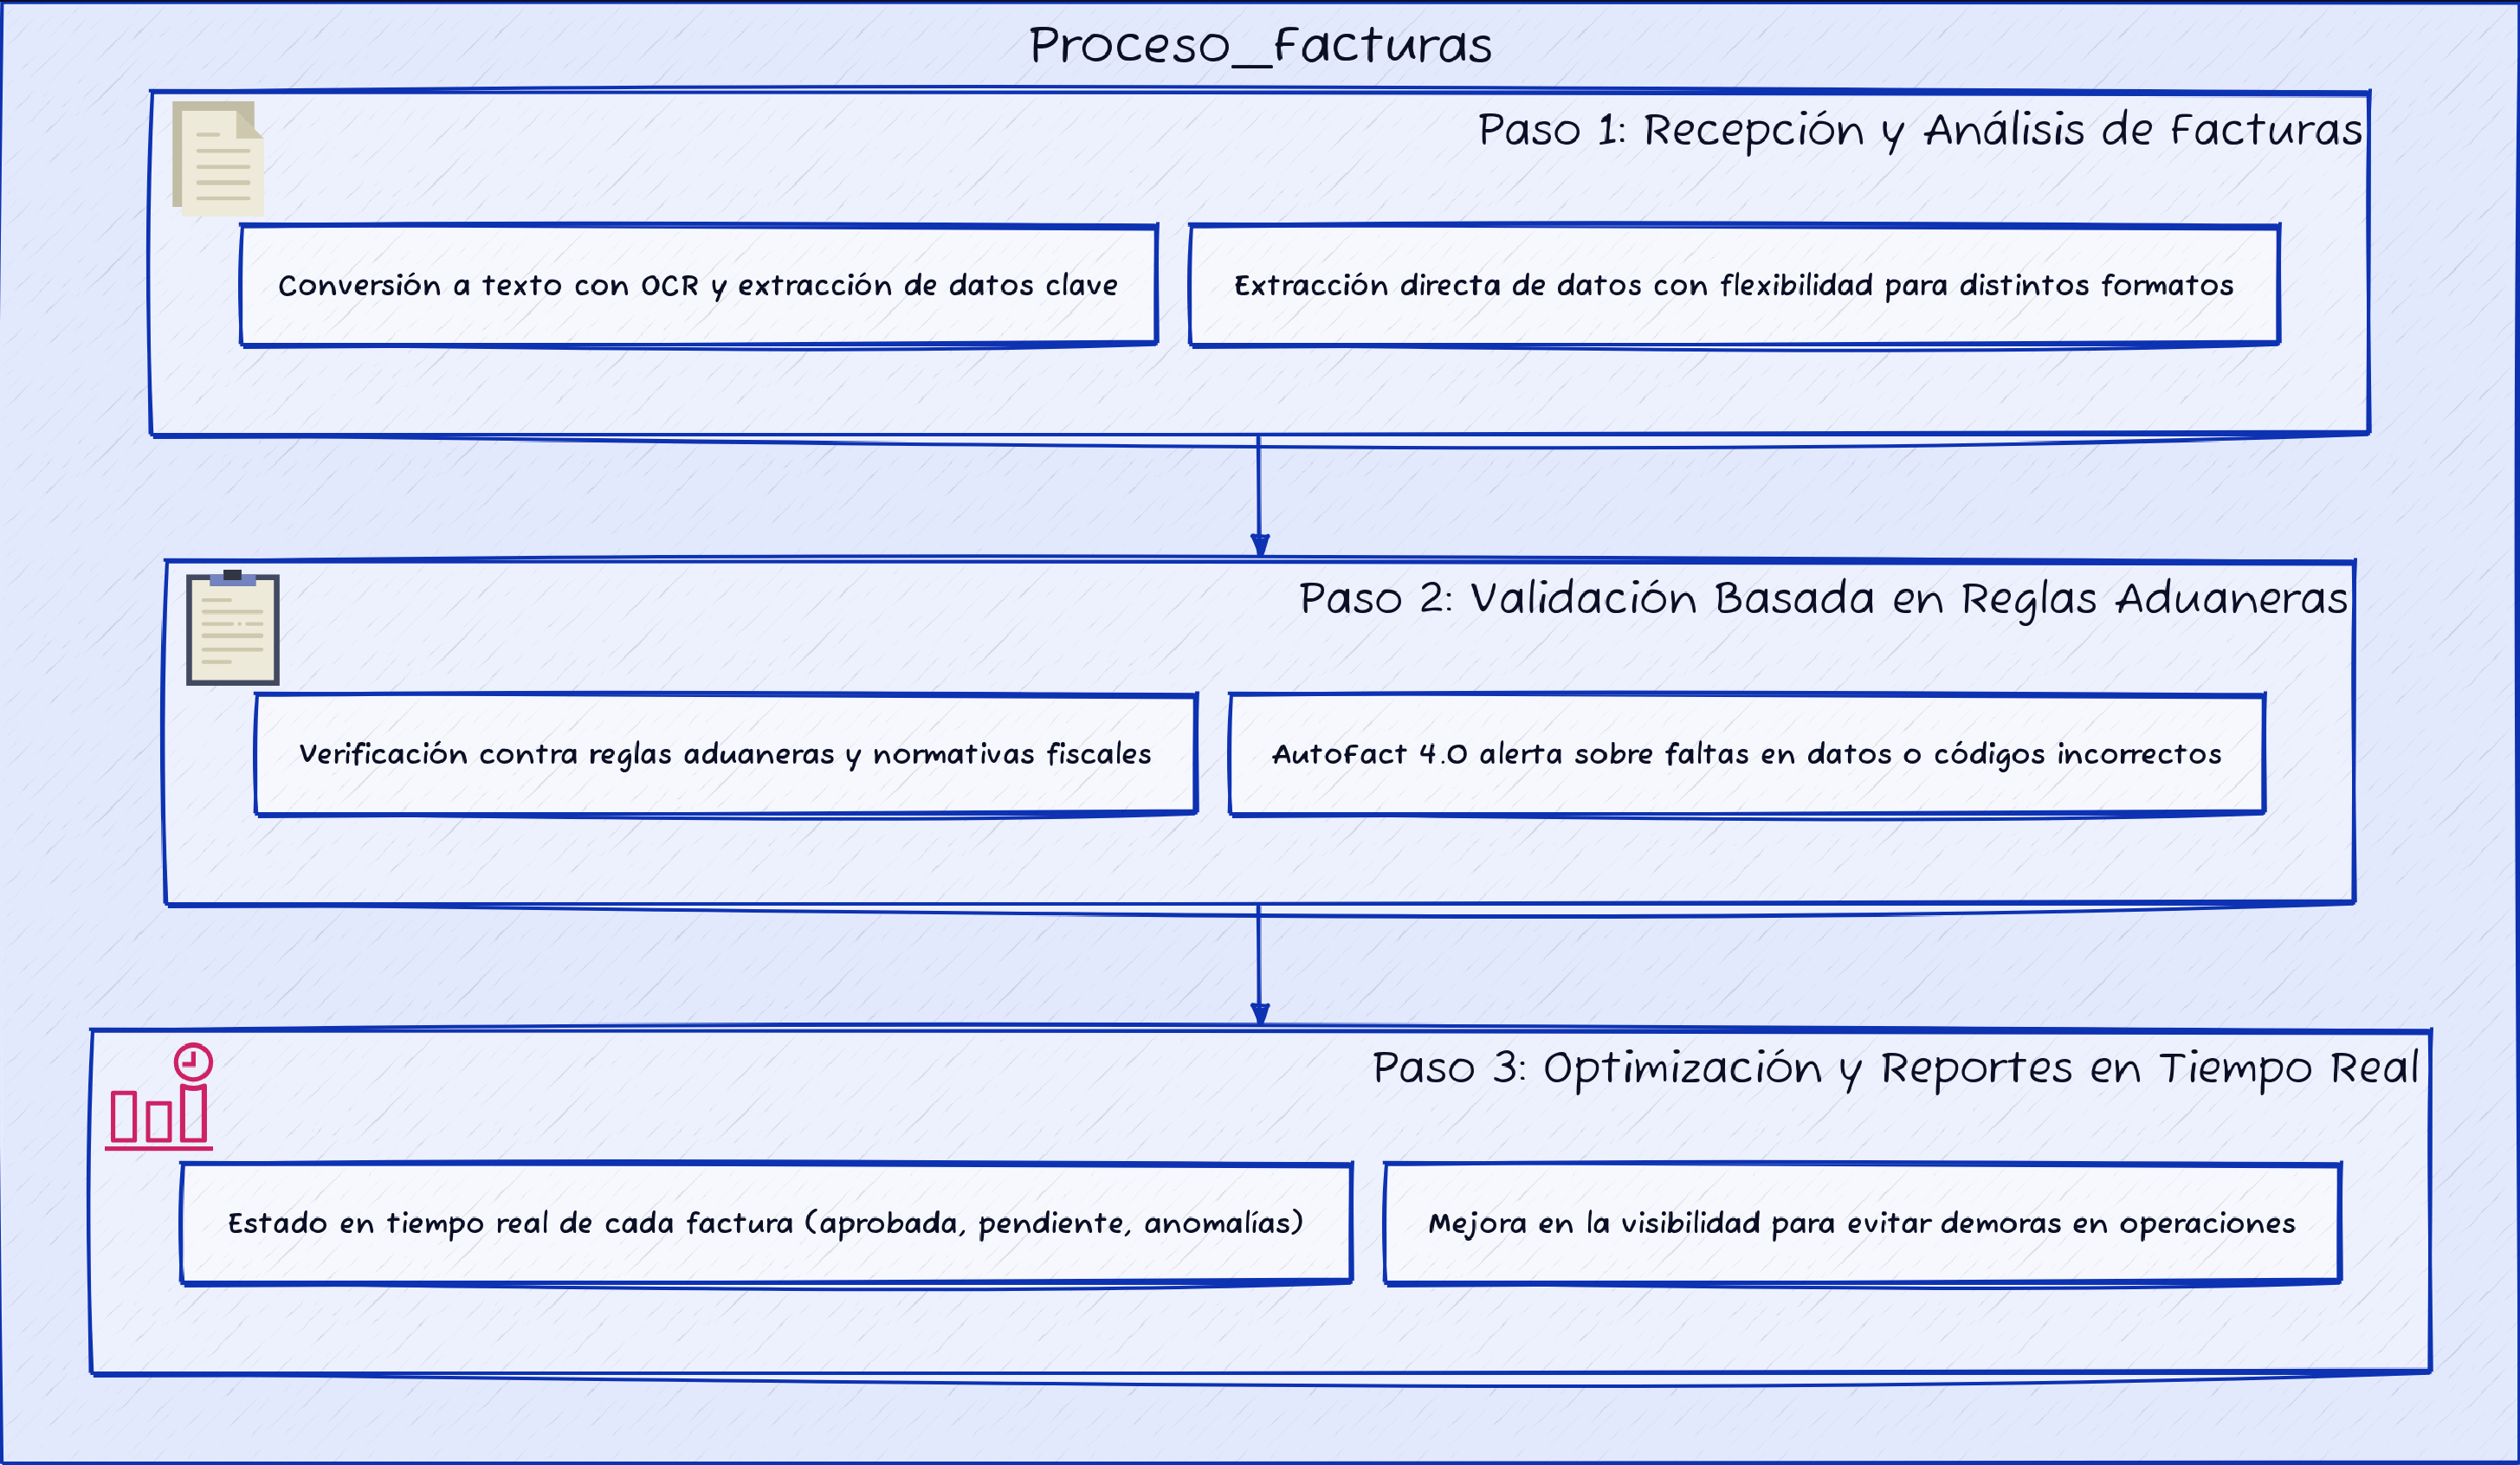
\includegraphics[width=1\textwidth,height=\textheight]{index_files/mediabag/diagram-5.pdf}

Ventajas de AutoFact 4.0

\textbf{1. Reducción de la Intervención Humana:} Con \textbf{AutoFact
4.0}, el número de capturistas se reduce drásticamente. De 100
capturistas a solo un equipo pequeño que supervise el sistema. Esto no
solo reduce costos laborales, sino que mejora la precisión y velocidad
del proceso.

\textbf{2. Integración con Normas Aduaneras:} Uno de los beneficios
clave de \textbf{AutoFact 4.0} es su capacidad para integrar reglas
aduaneras y normativas fiscales. Este sistema verifica automáticamente
que cada factura cumpla con las normativas vigentes, evitando errores
que podrían causar problemas legales o multas.

\textbf{3. Mayor Rapidez y Precisión:} Los modelos LLM permiten procesar
miles de facturas en minutos, con una precisión que reduce al mínimo los
errores humanos. La comunicación fluida entre \textbf{PDFs},
\textbf{XMLs} y los modelos permite optimizar el tiempo de respuesta.

\textbf{4. Escalabilidad:} A medida que la maquila crece,
\textbf{AutoFact 4.0} se adapta fácilmente a un mayor volumen de
facturas sin requerir una expansión significativa del equipo humano.

\subsubsection{Consideraciones
Técnicas}\label{consideraciones-tuxe9cnicas}

La implementación de \textbf{AutoFact 4.0} será un proyecto a largo
plazo debido a la complejidad de la \textbf{comunicación entre
diferentes formatos de facturas y los modelos LLM}. No es un simple
``plug and play''. El sistema deberá ser ajustado y optimizado para
funcionar sin problemas en todas las áreas de la maquila.

El proceso completo de implementación incluye:

\begin{enumerate}
\def\labelenumi{\arabic{enumi}.}
\tightlist
\item
  \textbf{Capacitación del equipo de TI} en el manejo de los modelos
  LLM.
\item
  \textbf{Ajuste de las reglas aduaneras} para cada caso particular de
  la maquiladora.
\item
  \textbf{Evaluaciones periódicas} para asegurar que el sistema esté
  funcionando de acuerdo con los parámetros establecidos.
\end{enumerate}

\subsubsection{Reflexión Final}\label{reflexiuxf3n-final-2}

\textbf{AutoFact 4.0} no solo agiliza el proceso de captura de facturas,
sino que representa un cambio en la forma en que las maquiladoras de
Juárez operan. Implementar un sistema de este tipo es un paso esencial
para mantenerse competitivos en un entorno cada vez más digitalizado y
globalizado. Con la capacidad de \textbf{procesar, validar y optimizar}
miles de facturas en cuestión de minutos, este modelo basado en
\textbf{LLM} es una herramienta poderosa para cualquier maquiladora que
busque reducir costos, mejorar la eficiencia y asegurar el cumplimiento
normativo.

\begin{longtable}[]{@{}
  >{\raggedright\arraybackslash}p{(\columnwidth - 4\tabcolsep) * \real{0.2300}}
  >{\raggedright\arraybackslash}p{(\columnwidth - 4\tabcolsep) * \real{0.1800}}
  >{\raggedright\arraybackslash}p{(\columnwidth - 4\tabcolsep) * \real{0.5900}}@{}}
\caption{Ranking de Adaptación a la IA para el Proyecto}\tabularnewline
\toprule\noalign{}
\begin{minipage}[b]{\linewidth}\raggedright
\textbf{Factor}
\end{minipage} & \begin{minipage}[b]{\linewidth}\raggedright
\textbf{Valor}
\end{minipage} & \begin{minipage}[b]{\linewidth}\raggedright
\textbf{Descripción}
\end{minipage} \\
\midrule\noalign{}
\endfirsthead
\toprule\noalign{}
\begin{minipage}[b]{\linewidth}\raggedright
\textbf{Factor}
\end{minipage} & \begin{minipage}[b]{\linewidth}\raggedright
\textbf{Valor}
\end{minipage} & \begin{minipage}[b]{\linewidth}\raggedright
\textbf{Descripción}
\end{minipage} \\
\midrule\noalign{}
\endhead
\bottomrule\noalign{}
\endlastfoot
\textbf{Complejidad Técnica} & Media (3) & Este proyecto requiere
conocimientos avanzados en programación, La integración de diferentes
formatos de archivos (PDF y XML) y la personalización de reglas
aduaneras lo hace un reto técnico considerable. Se necesitará un equipo
técnico especializado para su desarrollo e implementación. \\
\textbf{Tiempo de Implementación} & Largo (5) & Implementar
\textbf{AutoFact 4.0} tomará más de un año debido a la necesidad de
desarrollar la comunicación entre modelos LLM y los diferentes formatos
de facturas, pruebas exhaustivas, ajustes y capacitaciones. Además, será
necesario integrar el sistema con las plataformas actuales de la maquila
y ajustar las reglas de validación aduanera. \\
\textbf{Inversión Económica} & Alta (5) & Se requiere una inversión
considerable en tecnología (LLMs, servidores, software de OCR),
infraestructura y capacitación de personal. El costo inicial es alto,
pero se justifica por la reducción de costos operativos a largo plazo y
la mejora en la eficiencia y precisión de la captura de facturas. \\
\textbf{Capacitación y Adaptación del Personal} & Baja (1) & El personal
necesitará capacitación moderada en el uso de la nueva tecnología, sobre
todo en la supervisión y ajuste de las reglas aduaneras, así como en la
gestión del flujo de trabajo del sistema. No obstante, una parte
significativa del personal que antes realizaba tareas de captura manual
podría ser reasignada o necesitar nuevas habilidades. \\
\textbf{Impacto en la Cultura Organizacional} & Alto (5) & Este proyecto
tendrá un impacto profundo en la cultura organizacional, ya que
transformará completamente el proceso de captura de facturas, eliminando
tareas repetitivas y promoviendo una cultura más digital y automatizada.
Se requerirán ajustes en las políticas y procedimientos de la maquila
para alinearse con esta nueva forma de operar. \\
& & \\
\end{longtable}

\subsection{\texorpdfstring{Proyecto: \textbf{Generación Automática de
Bill of Materials (BOM)} para la
Maquiladora}{Proyecto: Generación Automática de Bill of Materials (BOM) para la Maquiladora}}\label{proyecto-generaciuxf3n-automuxe1tica-de-bill-of-materials-bom-para-la-maquiladora}

\subsubsection{Contexto en la
Maquiladora}\label{contexto-en-la-maquiladora}

La \textbf{Bill of Materials (BOM)} es el documento clave en cualquier
maquiladora, ya que detalla todos los materiales, piezas, subensambles y
procesos necesarios para fabricar un producto. En Ciudad Juárez, donde
la maquila es el motor económico, la precisión y velocidad en la
creación de la BOM son fundamentales para asegurar la continuidad en la
producción. Sin embargo, el proceso manual de generar una BOM puede ser
lento, costoso y propenso a errores. Las maquilas que dependen de
equipos de capturistas y especialistas en planeación pueden enfrentar
desafíos como errores humanos, falta de integración de datos entre
sistemas, y retrasos en la producción debido a la necesidad de revisar
manualmente diferentes documentos técnicos.

El proyecto de \textbf{Generación Automática de BOM} propone automatizar
este proceso utilizando \textbf{Modelos de Lenguaje Extensos (LLMs)} y
\textbf{procesamiento de lenguaje natural (NLP)} para analizar múltiples
formatos de documentos, como \textbf{imágenes CAD}, \textbf{archivos
PDF}, \textbf{XML}, y \textbf{Excel}, asegurando una extracción precisa
de los datos técnicos necesarios para crear la BOM. Esta automatización
reducirá significativamente el tiempo necesario para generar una BOM y
minimizará los errores humanos, aumentando la eficiencia y productividad
de la maquila.

\subsubsection{Objetivos del Proyecto}\label{objetivos-del-proyecto}

\begin{enumerate}
\def\labelenumi{\arabic{enumi}.}
\tightlist
\item
  \textbf{Automatizar la Generación de BOM:} Implementar un sistema de
  IA que procese automáticamente diferentes tipos de archivos para
  generar listas de materiales y componentes.
\item
  \textbf{Integración de Múltiples Formatos de Documentos:} Desarrollar
  la capacidad de analizar documentos en diversos formatos, como
  \textbf{CAD}, \textbf{PDF}, \textbf{XML}, y \textbf{Excel},
  garantizando la coherencia en la información extraída.
\item
  \textbf{Mejorar la Exactitud y Reducción de Errores:} Minimizar los
  errores humanos y asegurar la precisión en la generación de la BOM,
  eliminando discrepancias que podrían impactar la producción.
\item
  \textbf{Aceleración del Proceso de Producción:} Reducir el tiempo
  necesario para generar una BOM, optimizando el inicio de las
  actividades de compra y producción.
\end{enumerate}

\begin{longtable}[]{@{}
  >{\raggedright\arraybackslash}p{(\columnwidth - 4\tabcolsep) * \real{0.2300}}
  >{\raggedright\arraybackslash}p{(\columnwidth - 4\tabcolsep) * \real{0.1800}}
  >{\raggedright\arraybackslash}p{(\columnwidth - 4\tabcolsep) * \real{0.5900}}@{}}
\caption{Ranking de Adaptación a la IA para el Proyecto}\tabularnewline
\toprule\noalign{}
\begin{minipage}[b]{\linewidth}\raggedright
\textbf{Factor}
\end{minipage} & \begin{minipage}[b]{\linewidth}\raggedright
\textbf{Valor}
\end{minipage} & \begin{minipage}[b]{\linewidth}\raggedright
\textbf{Descripción}
\end{minipage} \\
\midrule\noalign{}
\endfirsthead
\toprule\noalign{}
\begin{minipage}[b]{\linewidth}\raggedright
\textbf{Factor}
\end{minipage} & \begin{minipage}[b]{\linewidth}\raggedright
\textbf{Valor}
\end{minipage} & \begin{minipage}[b]{\linewidth}\raggedright
\textbf{Descripción}
\end{minipage} \\
\midrule\noalign{}
\endhead
\bottomrule\noalign{}
\endlastfoot
\textbf{Complejidad Técnica} & Medio (3) & Se requiere el procesamiento
de múltiples formatos de archivos (CAD, PDF, XML, Excel, imágenes) y la
integración con plataformas ERP y sistemas CAD. Es un proyecto que
implica una alta demanda técnica. Pero la buena noticias si ya trabajas
con departo sera mucho mas rápido. agregar \\
\textbf{Tiempo de Implementación} & Media (2) & Se estima que el
proyecto podría tardar más de un 3 meses en completarse debido a la
complejidad de la integración de tecnologías y el desarrollo de un
protocolo de comunicación de IA adaptados a múltiples formatos de
archivos. \\
\textbf{Inversión Económica} & Media (3) & La inversión incluye costos
en infraestructura de TI, licencias de software especializado, y la
capacitación del personal en el uso de herramientas avanzadas de IA.
Además, se requiere de los modelos mas potentes de \textbf{OpenIA} y
\textbf{Google} grandes volúmenes de datos. \\
\textbf{Capacitación y Adaptación del Personal} & Medio (3) & El
personal técnico necesitará capacitación para comprender y gestionar el
sistema automatizado, pero el equipo de producción verá pocos cambios en
su flujo de trabajo, ya que la herramienta será amigable y accesible. \\
\textbf{Impacto en la Cultura Organizacional} & Medio (3) & La
automatización de la BOM afectará principalmente a los departamentos de
ingeniería y compras, pero se integrará en los procesos actuales sin
alterar drásticamente la estructura organizativa. \\
\end{longtable}

\subsubsection{Descripción del
Proyecto}\label{descripciuxf3n-del-proyecto}

La \textbf{Generación Automática de BOM} con IA utilizará \textbf{LLMs}
y \textbf{NLP} para interpretar diferentes formatos de documentos, como
\textbf{imágenes CAD}, \textbf{PDFs}, \textbf{XML}, y \textbf{hojas de
cálculo Excel}. El sistema extraerá la información necesaria para
construir una BOM precisa, como los materiales, componentes y
ensamblajes requeridos para la fabricación de un producto. Además, el
sistema permitirá la integración con sistemas ERP como \textbf{SAP},
facilitando la planificación de compras y el control de inventarios.

\subsubsection{Tipos de Formatos a
Procesar}\label{tipos-de-formatos-a-procesar}

\begin{enumerate}
\def\labelenumi{\arabic{enumi}.}
\item
  \textbf{Imágenes CAD:} Los diseños en \textbf{2D} y \textbf{3D} son
  fundamentales para la fabricación en la maquila. La IA será capaz de
  interpretar estos planos, identificando componentes y materiales
  directamente desde el diseño técnico.
\item
  \textbf{PDFs:} Documentos de especificaciones técnicas, manuales y
  planos en formato PDF contienen información crítica que la IA
  analizará para extraer detalles de materiales, tolerancias y procesos
  necesarios para la producción.
\item
  \textbf{XML:} Archivos XML, comúnmente utilizados en los procesos de
  facturación y en sistemas de gestión, serán interpretados para extraer
  datos sobre componentes y tiempos de entrega, conectando esta
  información con los sistemas ERP.
\item
  \textbf{Excel:} Muchas maquilas gestionan sus inventarios y listas de
  materiales en hojas de cálculo de Excel. La IA automatizará la
  interpretación de estos archivos, asegurando que los datos sean
  precisos y consistentes con la información técnica.
\item
  \textbf{Documentos Aduaneros:} Integrar el análisis de documentos
  aduaneros, como los reglamentos de exportación e importación, que
  afectan los componentes específicos que pueden utilizarse en la
  producción.
\end{enumerate}

\subsubsection{Proceso de
Implementación}\label{proceso-de-implementaciuxf3n}

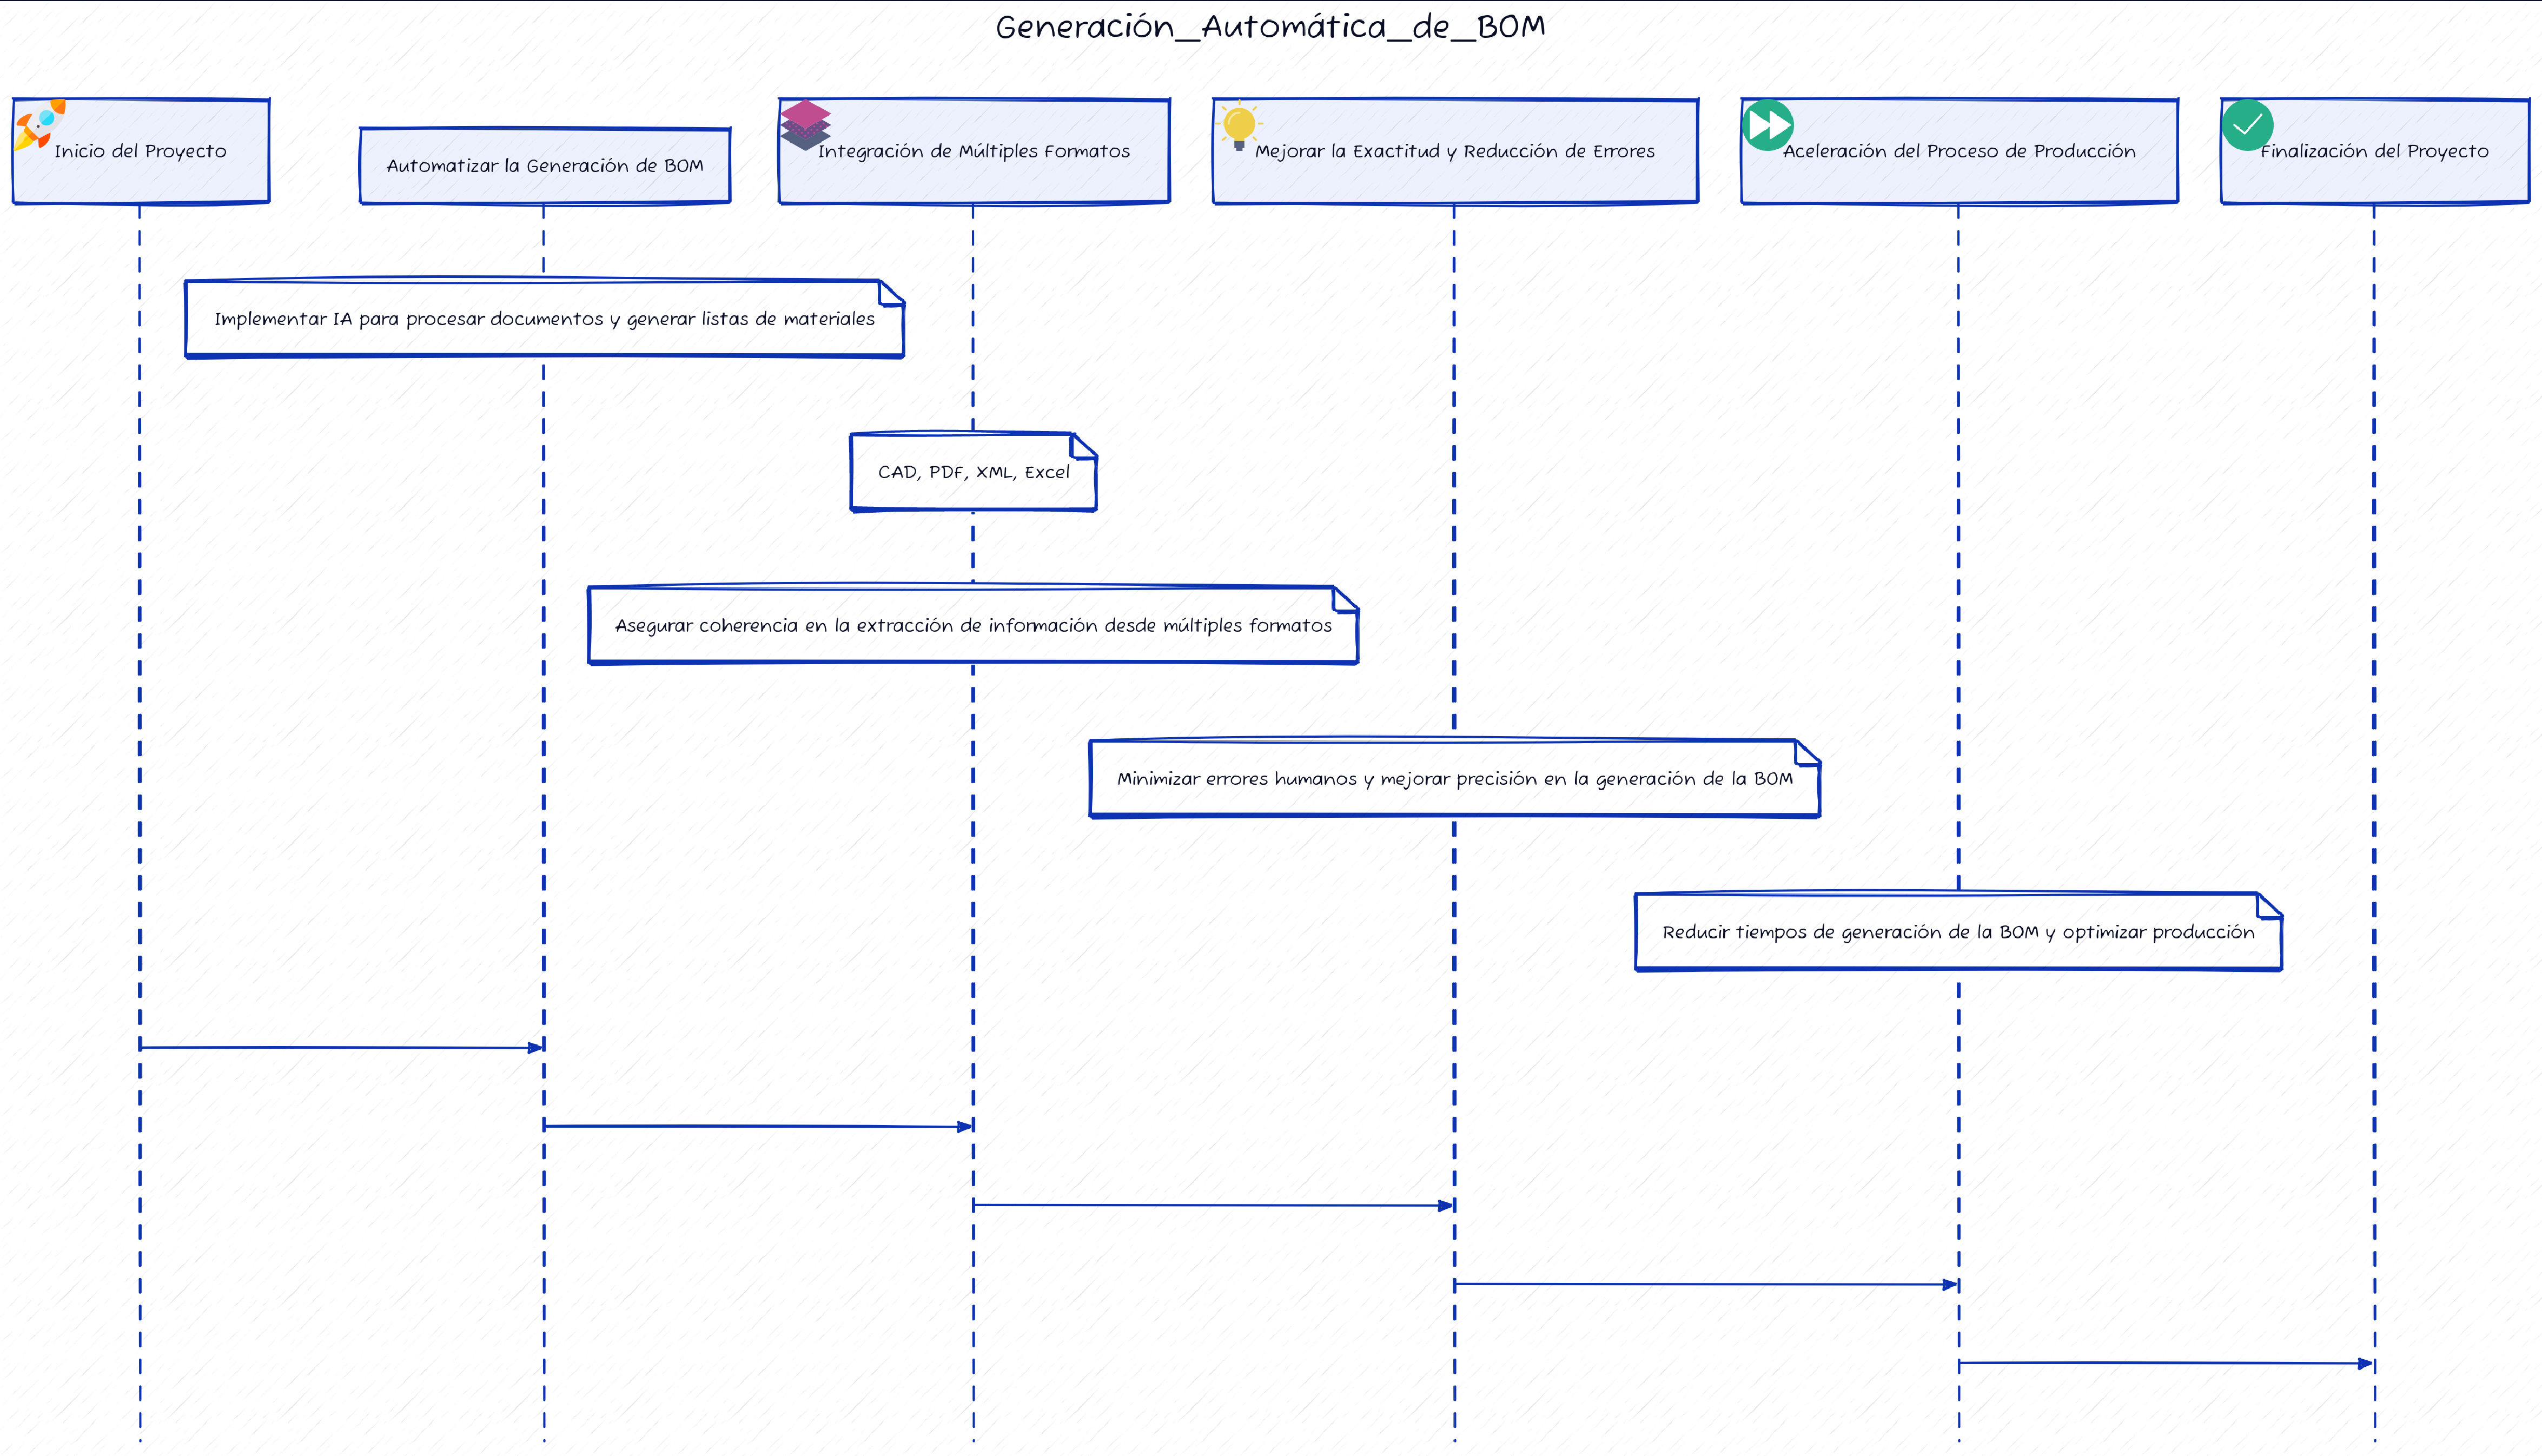
\includegraphics[width=1\textwidth,height=\textheight]{index_files/mediabag/diagram-6.pdf}

\begin{enumerate}
\def\labelenumi{\arabic{enumi}.}
\tightlist
\item
  \textbf{Recopilación de Documentos:} Los archivos CAD, PDFs, XML,
  Excel y otros documentos son cargados en el sistema para su
  procesamiento, Estos siguiendo con la lista de \textbf{BOM} de los
  análisis previos hechos a mano por los trabajores se recomienda uso
  minimo de 4 ejemplos por liena de producto.
\item
  \textbf{Análisis y Extracción de Datos:} El primer paso es la
  recepción de las fomratos. Estas llegan en diferentes formato Aquí
  entra en juego una etapa clave de la implementación: la capacidad del
  sistema para \textbf{comunicarse entre diferentes formatos y los
  LLM}.Toda esta comunicación sera usando \textbf{APIS} de estos
  modelos, Esto implica entrenar el modelo para que pueda interpretar
  estructuras variables de datos de los formatos.
\item
  \textbf{Generación de la BOM:} A partir de los datos extraídos, mas
  que nada los el modelos racionar por que los casos existosos fuero
  existoso y se genera automáticamente una BOM detallada que incluye
  todos los materiales y procesos necesarios para la fabricación del
  producto.
\item
  \textbf{Integración con ERP:} La BOM generada es enviada al sistema
  ERP (como \textbf{SAP}) para que el equipo de compras pueda proceder
  con la adquisición de los materiales.
\item
  \textbf{Actualización Continua:} A medida que se reciben nuevos
  diseños o se modifican las especificaciones, la BOM se actualiza
  automáticamente, manteniendo la coherencia en todas las fases del
  proceso.
\end{enumerate}

\subsubsection{Tecnologías Clave}\label{tecnologuxedas-clave}

\begin{itemize}
\tightlist
\item
  \textbf{LLMs (Large Language Models):} Modelos como \textbf{GPT-4} o
  \textbf{BERT} que interpretan texto y extraen información relevante de
  documentos en diferentes formatos.
\item
  \textbf{NLP (Natural Language Processing):} Procesamiento de lenguaje
  natural para interpretar las especificaciones técnicas de los
  documentos.
\item
  \textbf{Visión por Computadora:} La tecnología de visión por
  computadora permitirá analizar \textbf{imágenes CAD} y otros archivos
  gráficos, identificando componentes y ensamblajes automáticamente.
\item
  \textbf{Integración ERP y CAD:} Conectores para sistemas \textbf{ERP}
  y \textbf{CAD} (como \textbf{SAP} y \textbf{SolidWorks}) garantizarán
  que los datos fluyan sin problemas entre los sistemas de planificación
  y diseño.
\end{itemize}

\subsubsection{Desafíos y Soluciones}\label{desafuxedos-y-soluciones}

\begin{enumerate}
\def\labelenumi{\arabic{enumi}.}
\tightlist
\item
  \textbf{Desafío: Procesar múltiples formatos de archivo.}

  \begin{itemize}
  \tightlist
  \item
    \textbf{Solución:} Desarrollar un sistema recolección de archivos
    tanto textos como imágenes técnicas.
  \end{itemize}
\item
  \textbf{Desafío: Asegurar la precisión de la BOM generada.}

  \begin{itemize}
  \tightlist
  \item
    \textbf{Solución:} Implementar un proceso de revisión supervisada
    donde los ingenieros puedan validar los datos generados antes de
    enviarlos a producción.
  \end{itemize}
\item
  \textbf{Desafío: Integración con sistemas preexistentes (ERP y CAD).}

  \begin{itemize}
  \tightlist
  \item
    \textbf{Solución:} Desarrollar conectores específicos que permitan
    la interoperabilidad entre los sistemas ERP y CAD con el nuevo
    sistema de IA.
  \end{itemize}
\end{enumerate}

\subsubsection{Beneficios}\label{beneficios}

\begin{enumerate}
\def\labelenumi{\arabic{enumi}.}
\tightlist
\item
  \textbf{Reducción de Tiempos:} Al automatizar la creación de la BOM,
  se elimina la necesidad de que los capturistas analicen manualmente
  cada documento, acelerando el proceso de producción.
\item
  \textbf{Disminución de Errores:} La IA minimiza los errores humanos
  comunes en la creación de BOMs, como la omisión de componentes o
  materiales.
\item
  \textbf{Optimización de Recursos:} La integración directa con ERP
  asegura que los materiales se ordenen de manera oportuna y precisa,
  evitando retrasos en la producción.
\item
  \textbf{Escalabilidad:} El sistema es adaptable a cualquier volumen de
  producción y puede ajustarse rápidamente a nuevas líneas de productos
  o cambios en los procesos.
\end{enumerate}

\subsubsection{Conclusión}\label{conclusiuxf3n-2}

La implementación de un sistema de \textbf{Generación Automática de BOM}
utilizando IA representa un paso importante hacia la automatización y
eficiencia en la maquila. La capacidad de procesar múltiples formatos de
documentos, desde imágenes CAD hasta hojas de cálculo Excel, y generar
automáticamente listas de materiales precisas, asegura que las
maquiladoras puedan mantenerse competitivas en un mercado global que
demanda rapidez y precisión. Aunque la implementación es compleja y
requiere inversión, los beneficios a largo plazo, tanto en reducción de
costos como en mejora de eficiencia, son innegables.

\subsection{\texorpdfstring{Proyecto: \textbf{Creación de Interfaces de
Lenguaje Natural en la Pirámide de
Automatización}}{Proyecto: Creación de Interfaces de Lenguaje Natural en la Pirámide de Automatización}}\label{proyecto-creaciuxf3n-de-interfaces-de-lenguaje-natural-en-la-piruxe1mide-de-automatizaciuxf3n}

\textbf{Objetivo del Proyecto:}

El objetivo de este proyecto es revolucionar el manejo de los sistemas
de automatización industrial en la maquiladora mediante el uso de
\textbf{interfaces de lenguaje natural} (NLP por sus siglas en inglés),
eliminando la dependencia de expertos en SAP, SCADA Managers, o
ingenieros especializados en controladores. La idea es que cualquier
operador, gerente o supervisor pueda interactuar directamente con el
sistema a través de comandos sencillos y accesibles como: ``Quiero
producir lo mismo que ayer'' o ``Necesito hacer 100 piezas más'', sin
requerir un conocimiento técnico profundo.

Además, se integrarán funcionalidades para gestionar todos los niveles
de la \textbf{pirámide de automatización}, desde los
\textbf{controladores PLC y PID} hasta los sistemas de nivel superior
como \textbf{MES (Manufacturing Execution Systems)} y \textbf{SCADA}.
También se incluirán capacidades de monitoreo y mantenimiento predictivo
para identificar fallos en tiempo real y optimizar la operación en
planta.

\subsubsection{Introducción al
Problema}\label{introducciuxf3n-al-problema}

Actualmente, en muchas maquiladoras, las decisiones y ajustes de
producción requieren la intervención de varios expertos técnicos en
diferentes niveles de la pirámide de automatización. Esto genera cuellos
de botella y retrasa la producción, ya que muchas veces los operarios
deben esperar a que alguien especializado configure los sistemas o
interprete los datos de los controladores.

Con este proyecto, los trabajadores podrán interactuar directamente con
los sistemas de automatización mediante comandos simples y claros. No
hará falta un experto en SAP o SCADA para ajustar la producción o
interpretar datos de un PLC o controlador PID; todo será gestionado por
un modelo LLM (Large Language Model) que procesa el lenguaje natural y
ejecuta las órdenes o sugiere correcciones.

\subsubsection{Desglose de Niveles de la Pirámide de
Automatización}\label{desglose-de-niveles-de-la-piruxe1mide-de-automatizaciuxf3n}

\begin{enumerate}
\def\labelenumi{\arabic{enumi}.}
\item
  \textbf{Nivel de Campo (PLC y Controladores PID)}

  \begin{itemize}
  \item
    \textbf{Descripción:} En este nivel, los \textbf{PLC (Controladores
    Lógicos Programables)} y los \textbf{controladores PID} gestionan el
    control directo de máquinas y procesos. Estos dispositivos son
    fundamentales para asegurar que las operaciones se realicen
    correctamente, pero su monitoreo y ajuste suele requerir expertos en
    automatización industrial.
  \item
    \textbf{Monitoreo y Comandos:} Los usuarios podrán monitorear y
    gestionar los PLCs y PID a través de comandos de lenguaje natural
    como:

    \begin{itemize}
    \tightlist
    \item
      ``Quiero que la máquina mantenga la velocidad de producción de
      ayer.''
    \item
      ``Ajusta el controlador PID para reducir la variación en la
      temperatura del horno.''
    \item
      ``¿Está el PLC del equipo 2 funcionando correctamente?''
    \end{itemize}
  \item
    \textbf{Monitoreo de Fallos:} Los fallos en estos sistemas serán
    detectados automáticamente, y el sistema podrá responder con
    mensajes claros como: ``El PLC del equipo 3 ha fallado. Se
    recomienda revisión inmediata.''
  \item
    \textbf{Integración de APIs:} Las APIs conectarán directamente con
    los controladores para recibir información en tiempo real y permitir
    ajustes automáticos basados en las necesidades de producción.
  \end{itemize}
\item
  \textbf{Nivel de Supervisión (SCADA)}

  \begin{itemize}
  \item
    \textbf{Descripción:} El sistema \textbf{SCADA (Supervisory Control
    and Data Acquisition)} supervisa y controla procesos a nivel macro
    en la maquiladora. Actualmente, muchos supervisores necesitan
    conocimientos técnicos especializados para interactuar con estos
    sistemas.
  \item
    \textbf{Comandos de Lenguaje Natural:} Los operadores podrán
    interactuar directamente con SCADA mediante comandos simples,
    eliminando la necesidad de un especialista. Algunos ejemplos de
    comandos serían:

    \begin{itemize}
    \tightlist
    \item
      ``Quiero hacer 100 piezas más hoy.''
    \item
      ``Muestra el estado del sistema SCADA para la línea 4.''
    \item
      ``Ajusta la producción para alcanzar el objetivo de hoy.''
    \end{itemize}
  \item
    \textbf{Informes de Estado:} El sistema puede generar informes
    automáticos sobre el estado de la planta y sugiere ajustes si se
    detectan anomalías, por ejemplo: ``El nivel de producción está al
    80\%, se sugiere aumentar la velocidad de la línea 3.''
  \end{itemize}
\item
  \textbf{Nivel de Ejecución de la Producción (MES)}

  \begin{itemize}
  \item
    \textbf{Descripción:} El \textbf{MES (Manufacturing Execution
    System)} gestiona las operaciones de producción en tiempo real.
    Normalmente, su operación requiere personal capacitado para
    interactuar con la plataforma, analizar datos de producción y hacer
    ajustes basados en los resultados.
  \item
    \textbf{Comandos de Lenguaje Natural:} Con este proyecto, cualquier
    empleado podrá gestionar el MES de manera sencilla. Ejemplos de
    comandos:

    \begin{itemize}
    \tightlist
    \item
      ``Genera el reporte de scrap del turno matutino.''
    \item
      ``¿Cuántas piezas se produjeron ayer en la línea 2?''
    \item
      ``Optimiza el flujo de producción para evitar paros técnicos.''
    \end{itemize}
  \item
    \textbf{Integración de Datos:} Se integrarán los sistemas MES con el
    modelo LLM para proporcionar datos en tiempo real, sin necesidad de
    hojas de cálculo o sistemas externos complicados.
  \end{itemize}
\item
  \textbf{Nivel de Planificación (ERP)}

  \begin{itemize}
  \item
    \textbf{Descripción:} Los sistemas \textbf{ERP (Enterprise Resource
    Planning)} como SAP son los encargados de la planificación de
    recursos empresariales. Generalmente, interactuar con ellos requiere
    conocimientos avanzados y la intervención de expertos.
  \item
    \textbf{Comandos de Lenguaje Natural:} El sistema permitirá a los
    usuarios gestionar la planificación de recursos de manera sencilla,
    sin la necesidad de expertos en SAP. Ejemplos de comandos:

    \begin{itemize}
    \tightlist
    \item
      ``Planifica la producción de la próxima semana con base en la
      demanda actual.''
    \item
      ``Actualiza el inventario en el ERP con la producción de hoy.''
    \item
      ``Genera un reporte de las piezas producidas este mes.''
    \end{itemize}
  \item
    \textbf{Automatización de Flujos:} Este sistema permitirá
    automatizar la sincronización de datos entre el ERP y los niveles
    inferiores (MES, SCADA), facilitando la operación y planificación de
    manera más eficiente.
  \end{itemize}
\end{enumerate}

\subsubsection{Monitoreo y Reportes en Tiempo
Real}\label{monitoreo-y-reportes-en-tiempo-real}

El sistema también contará con la capacidad de monitorear el rendimiento
de los equipos en tiempo real y generar reportes automáticamente sobre
los problemas detectados. Por ejemplo, si un controlador PID o PLC
detecta una falla, el sistema alertará automáticamente y generará un
reporte en lenguaje natural. Estos reportes podrán incluir gráficos y
datos históricos para que los operadores puedan tomar decisiones
rápidamente.

Ejemplos de comandos para monitoreo y reportes: - ``Muestra el reporte
de scrap de la última semana.'' - ``¿Cuántas fallas ha tenido la línea
de producción en el mes?'' - ``Genera un informe de todas las órdenes
completadas en el turno nocturno.''

\subsubsection{Gestión de Scrap y
Reportes}\label{gestiuxf3n-de-scrap-y-reportes}

Otro aspecto clave será la capacidad del sistema para gestionar el scrap
y los reportes de producción. Normalmente, estos datos se registran
manualmente en hojas de cálculo o sistemas externos, lo que deja mucho
espacio para errores humanos. Con la integración de LLMs, cualquier
operador podrá registrar scrap o generar reportes de producción mediante
simples comandos de voz o texto.

Ejemplo de comando: - ``Registra 20 piezas como scrap en la línea 3.'' -
``Genera el reporte de eficiencia de producción del turno vespertino.''

\subsubsection{Detalle de los Módulos}\label{detalle-de-los-muxf3dulos}

\begin{enumerate}
\def\labelenumi{\arabic{enumi}.}
\tightlist
\item
  \textbf{Interfaz de Lenguaje Natural para PLC y PID}

  \begin{itemize}
  \tightlist
  \item
    Monitorea el estado de los controladores.
  \item
    Ajusta parámetros de manera automática con comandos simples.
  \item
    Reporta fallos y anomalías en tiempo real.
  \end{itemize}
\item
  \textbf{Interfaz para SCADA}

  \begin{itemize}
  \tightlist
  \item
    Genera reportes de estado y ajusta procesos.
  \item
    Controla el flujo de producción sin intervención de expertos.
  \item
    Optimiza operaciones a nivel de supervisión.
  \end{itemize}
\item
  \textbf{Interfaz para MES}

  \begin{itemize}
  \tightlist
  \item
    Facilita la gestión de la producción con comandos sencillos.
  \item
    Automatiza la generación de reportes y ajustes de líneas.
  \item
    Conecta con ERP para sincronización automática de datos.
  \end{itemize}
\item
  \textbf{Gestión de Scrap y Reportes}

  \begin{itemize}
  \tightlist
  \item
    Simplifica el registro y análisis de scrap.
  \item
    Genera reportes automáticos y gráficos visuales en tiempo real.
  \end{itemize}
\end{enumerate}

\subsubsection{Integración y
Flexibilidad}\label{integraciuxf3n-y-flexibilidad}

Todo este proyecto será soportado por un \textbf{dashboard interactivo},
donde se podrán visualizar los datos en tiempo real. La flexibilidad de
los LLMs permitirá que cualquier empleado --- desde el operador hasta el
gerente --- pueda gestionar procesos sin necesidad de intermediarios o
conocimientos técnicos avanzados. \textbf{No habrá más dependencia de
hojas de cálculo} ni expertos en SAP o SCADA. Toda la información fluirá
a través de un sistema centralizado y de fácil acceso.

\begin{longtable}[]{@{}
  >{\raggedright\arraybackslash}p{(\columnwidth - 4\tabcolsep) * \real{0.2300}}
  >{\raggedright\arraybackslash}p{(\columnwidth - 4\tabcolsep) * \real{0.1800}}
  >{\raggedright\arraybackslash}p{(\columnwidth - 4\tabcolsep) * \real{0.5900}}@{}}
\caption{Ranking de Adaptación a la IA para el Proyecto}\tabularnewline
\toprule\noalign{}
\begin{minipage}[b]{\linewidth}\raggedright
\textbf{Factor}
\end{minipage} & \begin{minipage}[b]{\linewidth}\raggedright
\textbf{Valor}
\end{minipage} & \begin{minipage}[b]{\linewidth}\raggedright
\textbf{Descripción}
\end{minipage} \\
\midrule\noalign{}
\endfirsthead
\toprule\noalign{}
\begin{minipage}[b]{\linewidth}\raggedright
\textbf{Factor}
\end{minipage} & \begin{minipage}[b]{\linewidth}\raggedright
\textbf{Valor}
\end{minipage} & \begin{minipage}[b]{\linewidth}\raggedright
\textbf{Descripción}
\end{minipage} \\
\midrule\noalign{}
\endhead
\bottomrule\noalign{}
\endlastfoot
\textbf{Complejidad Técnica} & Medio (3) & Aunque la integración de
varios sistemas es compleja, el uso de APIs y LLMs simplifica
enormemente la interacción para el usuario final. \\
\textbf{Tiempo de Implementación} & Medio (3) & Requiere un periodo de
implementación considerable, pero el resultado será una gestión
optimizada de la producción en meses. \\
\textbf{Inversión Económica} & Alta (4) & La inversión inicial es
significativa, especialmente en integración y capacitación, pero los
ahorros en tiempo y eficiencia lo compensan rápidamente. \\
\textbf{Capacitación y Adaptación del Personal} & Media (3) & La curva
de aprendizaje es baja gracias a las interfaces simples, pero se
necesitará algo de tiempo para que el personal se acostumbre a los
nuevos flujos de trabajo. \\
\textbf{Impacto en la Cultura Organizacional} & Alto (5) & Este proyecto
cambiará por completo la manera en que se gestiona \\
\end{longtable}

la producción en la maquila, con un impacto significativo en la
organización. Transformará la relación entre los operadores y los
sistemas de automatización. \textbar{}

Este proyecto no solo optimizará la gestión de la maquila, sino que
democratizará el acceso a la información y la toma de decisiones,
haciendo que cualquier trabajador pueda contribuir a la eficiencia de la
planta sin necesidad de expertos en SAP o SCADA. ¡La maquila del futuro
está más cerca de lo que pensamos!

\subsubsection{\texorpdfstring{\textbf{Advertencia Importante: Límites
de la
Implementación}}{Advertencia Importante: Límites de la Implementación}}\label{advertencia-importante-luxedmites-de-la-implementaciuxf3n}

Es esencial tener en cuenta que, aunque este proyecto va a transformar
la manera en que interactuamos con los sistemas de automatización en la
maquila, \textbf{no implicará que los sistemas se autoajusten
automáticamente sin supervisión humana}. Las \textbf{interfaces de
lenguaje natural (NLP)}, respaldadas por \textbf{modelos LLM},
facilitarán la comunicación entre el personal y los sistemas como los
\textbf{PLC}, \textbf{PID}, \textbf{SCADA}, \textbf{MES}, y
\textbf{ERP}, pero el control real de los procesos seguirá siendo
manejado por estos sistemas especializados. Esto es importante porque
\textbf{la lógica de control} de los procesos no será modificada por los
LLMs ni subida a la nube para realizar cambios automáticos.

La \textbf{inteligencia artificial no reemplazará el control directo de
la maquinaria} ni ajustará los parámetros críticos por su cuenta. En su
lugar, lo que haremos es \textbf{optimizar y simplificar la interacción}
con los sistemas ya existentes para que \textbf{cualquier usuario} pueda
manejar los procesos sin necesidad de depender de intermediarios
especializados como los \textbf{SAP Experts} o \textbf{SCADA Managers}.

\subsubsection{Detalles del Proyecto: Interfaz y
Limitaciones}\label{detalles-del-proyecto-interfaz-y-limitaciones}

\subsubsection{\texorpdfstring{1. \textbf{Interfaz para Controladores
PLC y
PID}}{1. Interfaz para Controladores PLC y PID}}\label{interfaz-para-controladores-plc-y-pid}

\begin{itemize}
\tightlist
\item
  \textbf{Función Principal:} Los operadores podrán ajustar los
  parámetros de los PLCs y PIDs mediante comandos sencillos como
  ``Ajusta la velocidad de la línea 2 para igualar la producción de
  ayer'' o ``¿Está funcionando correctamente el PLC de la línea 3?''.
\item
  \textbf{Límites:} Aunque el sistema podrá alertar sobre posibles
  fallos o parámetros fuera de rango, \textbf{no hará ajustes
  automáticos en la lógica de control} de los PLCs ni alterará los
  parámetros sin la autorización explícita del operador. Esto es crítico
  para asegurar que los cambios se realicen bajo la supervisión adecuada
  y que \textbf{no se comprometa la seguridad} de los procesos de
  manufactura.
\end{itemize}

\subsubsection{\texorpdfstring{2. \textbf{Interfaz
SCADA}}{2. Interfaz SCADA}}\label{interfaz-scada}

\begin{itemize}
\tightlist
\item
  \textbf{Función Principal:} La interfaz SCADA permitirá a los usuarios
  supervisar y controlar los procesos en la planta con comandos
  sencillos, como ``Genera un informe del estado de la línea de
  producción 4'' o ``Ajusta la producción para completar las metas del
  día''.
\item
  \textbf{Límites:} El SCADA seguirá gestionando el control en tiempo
  real y la adquisición de datos, pero \textbf{no se permitirá la
  modificación automática de las reglas de seguridad ni la creación de
  nuevas lógicas de control}. El modelo LLM únicamente servirá como
  puente para traducir las órdenes de los operadores en acciones,
  garantizando que se respeten los parámetros establecidos por los
  ingenieros de control.
\end{itemize}

\subsubsection{\texorpdfstring{3. \textbf{Interfaz MES para Producción y
Reportes}}{3. Interfaz MES para Producción y Reportes}}\label{interfaz-mes-para-producciuxf3n-y-reportes}

\begin{itemize}
\tightlist
\item
  \textbf{Función Principal:} El sistema permitirá la interacción con el
  \textbf{MES} de forma que cualquier empleado, sin ser experto en
  tecnología, pueda generar reportes o ajustar la programación de la
  producción. Comandos como ``Genera el reporte de scrap del turno
  vespertino'' o ``Aumenta la producción de la línea 1 para alcanzar el
  objetivo de la semana'' serán posibles.
\item
  \textbf{Límites:} La IA no modificará las reglas de negocio ni el
  flujo de trabajo por sí misma. La lógica del MES, como los tiempos de
  producción o los inventarios, \textbf{no será alterada sin
  intervención humana}. Los usuarios seguirán tomando las decisiones
  clave, y la IA solo actuará como un asistente que simplifica la
  interacción.
\end{itemize}

\subsubsection{\texorpdfstring{4. \textbf{Interfaz para ERP (SAP y
otros)}}{4. Interfaz para ERP (SAP y otros)}}\label{interfaz-para-erp-sap-y-otros}

\begin{itemize}
\tightlist
\item
  \textbf{Función Principal:} El ERP gestionará la planificación de
  recursos de la empresa y se integrará perfectamente con el MES y SCADA
  para garantizar que las órdenes de producción y los inventarios estén
  sincronizados. Comandos como ``Planifica la producción para el próximo
  mes en base a los niveles actuales de inventario'' o ``Actualiza los
  datos del ERP con las órdenes de hoy'' serán fácilmente ejecutables.
\item
  \textbf{Límites:} La planificación de recursos empresariales, como la
  asignación de inventarios o la generación de órdenes de compra,
  \textbf{no será modificada automáticamente por la IA}. El ERP
  continuará operando bajo las reglas definidas por los gerentes y
  especialistas, asegurando que no se introduzcan errores o decisiones
  inadecuadas.
\end{itemize}

\subsubsection{Gestión de Datos: Sin Subida a la
Nube}\label{gestiuxf3n-de-datos-sin-subida-a-la-nube}

Uno de los aspectos críticos de este proyecto es que \textbf{ningún dato
sensible o crítico de la producción será subido a la nube}. Todos los
procesos, desde el monitoreo de los PLCs hasta la generación de reportes
en el MES, se realizarán de forma local en la maquila. La razón detrás
de esta decisión es doble:

\begin{enumerate}
\def\labelenumi{\arabic{enumi}.}
\item
  \textbf{Seguridad y Cumplimiento Normativo:} La mayoría de las
  maquiladoras operan bajo estrictas regulaciones de seguridad y
  confidencialidad, y subir los datos de producción a la nube podría
  poner en riesgo la operación o incluso infringir normativas locales o
  internacionales.
\item
  \textbf{Control Total sobre los Procesos:} Al mantener la operación
  dentro de la planta, se garantiza que el control siempre permanezca en
  manos del equipo humano, evitando depender de conexiones externas o de
  infraestructuras en la nube que puedan ser vulnerables a fallos.
\end{enumerate}

\subsubsection{Módulos de Supervisión: Dashboard
Centralizado}\label{muxf3dulos-de-supervisiuxf3n-dashboard-centralizado}

El sistema incluirá un \textbf{dashboard interactivo centralizado} donde
los operadores, supervisores, y gerentes podrán monitorear en tiempo
real todos los sistemas (PLC, SCADA, MES, ERP) sin necesidad de hojas de
cálculo ni documentos externos. Este dashboard estará diseñado para ser
\textbf{intuitivo y accesible}, permitiendo que cualquier persona, sin
importar su nivel de experiencia, pueda visualizar datos críticos y
tomar decisiones informadas. Además:

\begin{itemize}
\tightlist
\item
  \textbf{Visualización en Tiempo Real:} El dashboard mostrará gráficos
  de tendencias de producción, rendimiento de máquinas, scrap y otros
  indicadores clave.
\item
  \textbf{Alertas Automatizadas:} Si ocurre un fallo en un PLC o un
  nivel de producción cae por debajo de lo esperado, el sistema emitirá
  alertas automáticas, notificando al personal adecuado para que tome
  acción.
\item
  \textbf{Generación de Reportes Personalizados:} Los usuarios podrán
  generar reportes con un solo clic o comando, permitiendo que incluso
  los operadores menos experimentados puedan realizar reportes
  detallados sin complicaciones.
\end{itemize}

\subsubsection{Niveles de Acceso: Diferenciación de
Roles}\label{niveles-de-acceso-diferenciaciuxf3n-de-roles}

El proyecto también contemplará un sistema de \textbf{niveles de acceso}
que diferenciará los roles de cada usuario en la maquila. Los operadores
podrán gestionar tareas operativas simples, mientras que los
supervisores y gerentes tendrán acceso a funciones más avanzadas. Esta
diferenciación garantiza que el control total de la producción esté en
manos de quienes tienen la autoridad y la experiencia necesaria para
tomar decisiones estratégicas.

Ejemplo de Comandos por Rol:

\begin{itemize}
\tightlist
\item
  \textbf{Operador:} ``Genera un reporte de scrap de hoy'' o ``Aumenta
  la velocidad de producción en la línea 2.''
\item
  \textbf{Supervisor:} ``Optimiza la producción para cumplir con la meta
  semanal'' o ``Ajusta el flujo de trabajo en base a los últimos
  reportes.''
\item
  \textbf{Gerente:} ``Planifica la producción para el próximo
  trimestre'' o ``Genera un análisis de desempeño de todas las líneas de
  producción este mes.''
\end{itemize}

\subsubsection{Conclusión y Beneficios Clave del
Proyecto}\label{conclusiuxf3n-y-beneficios-clave-del-proyecto}

Este proyecto representa un salto significativo en la forma en que las
maquiladoras gestionan sus procesos. Al integrar LLMs y
\textbf{interfaces de lenguaje natural} en todos los niveles de la
pirámide de automatización, se democratiza el acceso a la información y
se simplifica la operación, permitiendo que cualquier persona en la
organización pueda interactuar de manera eficiente con sistemas
complejos sin necesidad de expertos intermediarios.

\textbf{Beneficios Clave:} - \textbf{Facilidad de Uso:} No se requerirán
expertos en SAP, SCADA, o MES para gestionar la producción. Los comandos
simples en lenguaje natural harán que cualquier usuario pueda
interactuar con los sistemas de automatización. - \textbf{Reducción de
Errores:} Al eliminar la necesidad de hojas de cálculo y procesos
manuales, se minimizarán los errores humanos. - \textbf{Seguridad:}
Todos los datos se manejarán localmente, asegurando que no se suba
información crítica a la nube, lo que garantiza el cumplimiento
normativo y la protección de los datos de producción. - \textbf{Mayor
Eficiencia:} La rapidez en la toma de decisiones mejorará la eficiencia
operativa, ya que los sistemas responderán de manera inmediata a las
órdenes de los operadores. - \textbf{Flexibilidad:} El sistema permitirá
ajustes en tiempo real sin la necesidad de realizar cambios en la lógica
de control, manteniendo la seguridad y estabilidad de los procesos.

En resumen, esta es una solución integral que moderniza la operación de
las maquiladoras, haciéndolas más eficientes, accesibles y seguras, con
una mínima dependencia de expertos técnicos. ¡Todo el control estará en
manos de la maquila!

\subsection{\texorpdfstring{Proyecto Estrella: \textbf{LLMs en la
Gestión de la Cadena de Suministro con Dashboard
Interactivo}}{Proyecto Estrella: LLMs en la Gestión de la Cadena de Suministro con Dashboard Interactivo}}\label{proyecto-estrella-llms-en-la-gestiuxf3n-de-la-cadena-de-suministro-con-dashboard-interactivo}

\subsubsection{Ejemplo del Problema Actual en la
Maquiladora}\label{ejemplo-del-problema-actual-en-la-maquiladora}

Imagina que tienes una maquila que fabrica componentes electrónicos, con
un flujo constante de partes que llegan de diferentes proveedores
alrededor del mundo. Tienes a más de 100 capturistas revisando facturas,
órdenes de compra y registros de inventario a diario, pero la
información está dispersa en hojas de cálculo, PDFs y hasta imágenes
escaneadas. Esto genera errores, procesos lentos, y decisiones basadas
en suposiciones. El problema se agrava cuando la demanda cambia
repentinamente o los proveedores no cumplen con los tiempos de entrega,
afectando tu producción.

En este escenario, los Modelos de Lenguaje Extenso (LLMs) llegan para
resolver este caos. Con los módulos que describiremos a continuación, no
necesitarás ni siquiera usar una hoja de cálculo. Todo será gestionado y
optimizado automáticamente, permitiendo que cualquier persona --- desde
un gerente hasta un operador de línea --- pueda interactuar con los
sistemas a través de un \textbf{dashboard intuitivo}. Olvídate de
depender de expertos en SAP o intermediarios que complican los procesos.
Con LLMs, la gestión de la cadena de suministro será tan sencilla como
hacerle una pregunta a tu asistente virtual.

\subsubsection{Objetivos del Proyecto}\label{objetivos-del-proyecto-1}

\begin{enumerate}
\def\labelenumi{\arabic{enumi}.}
\tightlist
\item
  \textbf{Prever la demanda con precisión}: A través del análisis de
  datos históricos y tendencias de mercado, los LLMs pueden predecir de
  manera precisa la demanda, ajustando la producción e inventarios sin
  intervención manual.
\item
  \textbf{Automatizar la evaluación de proveedores}: El sistema
  analizará en tiempo real los datos de los proveedores y te dará una
  evaluación clara y objetiva sin necesidad de hojas de cálculo o
  análisis manual.
\item
  \textbf{Optimizar inventarios y costos}: El sistema ajustará los
  niveles de inventario de manera automática, asegurando que nunca
  falten ni sobren productos.
\item
  \textbf{Dashboard interactivo y de fácil uso}: Todo centralizado en un
  tablero interactivo donde podrás consultar toda la información sin
  necesidad de hojas de Excel, PDFs, o sistemas complejos.
\end{enumerate}

\subsubsection{Módulos del Proyecto con
Dashboard}\label{muxf3dulos-del-proyecto-con-dashboard}

\begin{enumerate}
\def\labelenumi{\arabic{enumi}.}
\tightlist
\item
  \textbf{Predicción de la Demanda con LLMs}
\end{enumerate}

\textbf{Descripción:} Utilizando LLMs, este módulo analiza grandes
volúmenes de datos históricos, tendencias de mercado y factores externos
(como clima o eventos globales) para predecir la demanda futura. Con
esta información, el sistema ajusta automáticamente las órdenes de
producción y los niveles de inventario, sin necesidad de que nadie toque
una hoja de cálculo.

\textbf{Ejemplo de Uso:} Supongamos que el mercado global está
fluctuando por cambios económicos. El gerente le pide al sistema que
proyecte las necesidades de producción para los próximos seis meses
basándose en ventas anteriores y las tendencias actuales del mercado. El
sistema no solo le proporciona un análisis detallado, sino que ajusta
automáticamente las órdenes de compra necesarias.

\textbf{Dashboard:} El tablero mostrará gráficos en tiempo real con las
proyecciones de demanda y los ajustes de inventario recomendados.
Además, enviará alertas automáticas si se detectan fluctuaciones que
puedan afectar la producción.

\textbf{Beneficios Clave:} - Reducción de sobre producción y escasez de
inventario. - Ajustes automáticos en la planificación de la producción.
- Decisiones rápidas y precisas, sin necesidad de hojas de cálculo.

\textbf{Posición Asignada:} \textbf{Especialista en Predicción de
Demanda con IA}

\begin{enumerate}
\def\labelenumi{\arabic{enumi}.}
\setcounter{enumi}{1}
\tightlist
\item
  \textbf{Evaluación Automática de Proveedores}
\end{enumerate}

\textbf{Descripción:} Este módulo utiliza LLMs para analizar datos de
rendimiento de proveedores (calidad, tiempos de entrega, costos) y
generar un ranking automático sin intervención manual. El sistema
compara en tiempo real a todos los proveedores y sugiere automáticamente
aquellos que cumplen con los mejores estándares, sin depender de largas
hojas de cálculo ni de personal especializado.

\textbf{Ejemplo de Uso:} Un operador ingresa una nueva orden de compra
para componentes clave. El sistema ya ha evaluado todos los proveedores
disponibles y sugiere el mejor en términos de costo y tiempo de entrega,
actualizando automáticamente el ranking de proveedores.

\textbf{Dashboard:} El tablero presentará una vista clara del
rendimiento de todos los proveedores en un gráfico comparativo. También
mostrará alertas si algún proveedor ha tenido problemas recientes de
calidad o tiempos de entrega.

\textbf{Beneficios Clave:} - Decisiones objetivas basadas en datos
duros. - Eliminación de errores humanos y sesgos en la evaluación de
proveedores. - Gestión automatizada sin necesidad de intermediarios o
análisis manual.

\textbf{Posición Asignada:} \textbf{Analista de Proveedores con IA}

\begin{enumerate}
\def\labelenumi{\arabic{enumi}.}
\setcounter{enumi}{2}
\tightlist
\item
  \textbf{Optimización de Inventarios con LLMs}
\end{enumerate}

\textbf{Descripción:} Los LLMs optimizan los niveles de inventario
analizando las tasas de rotación, los tiempos de entrega de los
proveedores y los patrones de consumo. El sistema ajusta automáticamente
las órdenes de compra y reduce los costos de almacenamiento, todo sin
necesidad de que nadie ingrese datos manualmente.

\textbf{Ejemplo de Uso:} El sistema detecta que el consumo de un
componente clave está aumentando y ajusta automáticamente el pedido para
evitar que te quedes sin stock. Todo esto sin una sola hoja de Excel
involucrada.

\textbf{Dashboard:} Podrás visualizar en tiempo real los niveles de
inventario y las proyecciones de consumo, con alertas automáticas para
optimizar los pedidos y evitar sobre costos o quiebres de stock.

\textbf{Beneficios Clave:} - Reducción de costos de almacenamiento. -
Evita quiebres de stock críticos. - Gestión automática sin hojas de
cálculo o sistemas externos complicados.

\textbf{Posición Asignada:} \textbf{Gerente de Inventario Inteligente}

\paragraph{\texorpdfstring{4. \textbf{Automatización del BOM (Bill of
Materials)}}{4. Automatización del BOM (Bill of Materials)}}\label{automatizaciuxf3n-del-bom-bill-of-materials}

\textbf{Descripción:} Genera automáticamente el \textbf{Bill of
Materials (BOM)} a partir de múltiples formatos como imágenes CAD, PDFs,
y hojas de cálculo. El sistema extrae toda la información necesaria y
crea un BOM completo sin necesidad de validaciones manuales o
intermediarios.

\textbf{Ejemplo de Uso:} El ingeniero sube un diseño en formato CAD, y
el sistema automáticamente genera la lista de materiales necesaria,
ajustando los pedidos y sugiriendo los mejores proveedores. No hace
falta ni abrir una hoja de Excel.

\textbf{Dashboard:} El dashboard mostrará una vista completa del BOM,
junto con las proyecciones de costos, tiempos de entrega y proveedores
sugeridos. Todo de manera visual y accesible desde cualquier
dispositivo.

\textbf{Beneficios Clave:} - Ahorro de tiempo en la creación del BOM. -
Eliminación de errores humanos en la recopilación de datos. -
Automatización total sin necesidad de hojas de cálculo ni validaciones
manuales.

\textbf{Posición Asignada:} \textbf{Ingeniero de Automatización del BOM}

\paragraph{\texorpdfstring{5. \textbf{Interacción con la Cadena de
Suministro a través de Lenguaje
Natural}}{5. Interacción con la Cadena de Suministro a través de Lenguaje Natural}}\label{interacciuxf3n-con-la-cadena-de-suministro-a-travuxe9s-de-lenguaje-natural}

\textbf{Descripción:} Este módulo permite que cualquier persona en la
maquila, desde operadores hasta gerentes, pueda interactuar con el
sistema usando lenguaje natural. Esto significa que puedes hacerle
preguntas directamente al sistema sin tener que saber nada de SAP, hojas
de cálculo, o programación avanzada.

\textbf{Ejemplo de Uso:} Un operador puede preguntarle al sistema:
``¿Cuánto inventario tenemos del componente X?'' y recibir
inmediatamente una respuesta acompañada de gráficos y recomendaciones
sin tener que abrir ni un solo archivo.

\textbf{Dashboard:} El tablero incluye una sección de \textbf{Input de
Lenguaje Natural} donde los usuarios pueden hacer preguntas o
solicitudes directamente al sistema y recibir respuestas claras en
tiempo real.

\textbf{Beneficios Clave:} - Cualquiera puede usarlo, desde gerentes
hasta operadores. - No se requieren conocimientos técnicos o de sistemas
complicados. - Acceso rápido y directo a información crítica.

\textbf{Posición Asignada:} \textbf{Desarrollador de Interacción con IA}

\subsubsection{Ventajas del Proyecto}\label{ventajas-del-proyecto}

\begin{enumerate}
\def\labelenumi{\arabic{enumi}.}
\item
  \textbf{Cero Uso de Hojas de Cálculo:} Todos los procesos se gestionan
  desde el dashboard interactivo y a través del procesamiento en
  lenguaje natural, eliminando la necesidad de hojas de cálculo o
  sistemas externos como SAP.
\item
  \textbf{Optimización de Decisiones:} Las decisiones clave se toman
  basadas en datos analizados automáticamente por LLMs, sin sesgos ni
  errores humanos, lo que mejora la eficiencia y la precisión.
\item
  \textbf{Facilidad de Uso para Todos:} Desde operadores hasta gerentes,
  todos pueden interactuar con el sistema sin necesidad de conocimientos
  técnicos, utilizando únicamente lenguaje natural.
\item
  \textbf{Reducción de Costos:} Al automatizar la optimización de
  inventarios, la predicción de la demanda y la evaluación de
  proveedores, se eliminan los costos innecesarios de almacenamiento,
  pedidos erróneos, y sobreproducción.
\item
  \textbf{Dashboard Centralizado y Visualización Clara:} El dashboard
  interactivo permite tener toda la información en tiempo real,
  accesible y visualizada de manera sencilla, facilitando la toma de
  decisiones.
\end{enumerate}

\begin{longtable}[]{@{}
  >{\raggedright\arraybackslash}p{(\columnwidth - 4\tabcolsep) * \real{0.2300}}
  >{\raggedright\arraybackslash}p{(\columnwidth - 4\tabcolsep) * \real{0.1800}}
  >{\raggedright\arraybackslash}p{(\columnwidth - 4\tabcolsep) * \real{0.5900}}@{}}
\caption{Ranking de Adaptación a la IA para el Proyecto}\tabularnewline
\toprule\noalign{}
\begin{minipage}[b]{\linewidth}\raggedright
Factor
\end{minipage} & \begin{minipage}[b]{\linewidth}\raggedright
Valor
\end{minipage} & \begin{minipage}[b]{\linewidth}\raggedright
Descripción
\end{minipage} \\
\midrule\noalign{}
\endfirsthead
\toprule\noalign{}
\begin{minipage}[b]{\linewidth}\raggedright
Factor
\end{minipage} & \begin{minipage}[b]{\linewidth}\raggedright
Valor
\end{minipage} & \begin{minipage}[b]{\linewidth}\raggedright
Descripción
\end{minipage} \\
\midrule\noalign{}
\endhead
\bottomrule\noalign{}
\endlastfoot
Complejidad Técnica & \textbf{Alto (5)} & Requiere una alta integración
de sistemas, pero su uso es fácil para cualquier persona. \\
Tiempo de Implementación & \textbf{Largo (5)} & El proyecto completo
puede llevar más de un año, pero las primeras fases ya muestran
resultados en menos de seis meses. \\
Inversión Económica & \textbf{Alta (5)} & Requiere inversión en
tecnología de IA, desarrollo de software y capacitación, pero el retorno
de inversión es rápido y claro. \\
Capacitación y Adaptación del Personal & \textbf{Media (3)} & Aunque el
sistema es muy intuitivo, necesitarás tiempo para que el personal se
adapte a las nuevas herramientas y funciones de interacción con IA. \\
Impacto en la Cultura Organizacional & \textbf{Alto (5)} & Implica un
cambio profundo en cómo se gestionan datos y decisiones, transformando
radicalmente la forma en que la maquila opera a nivel de gestión y
operatividad. Este proyecto no solo mejora la eficiencia operativa, sino
que también democratiza el uso de la IA, permitiendo que cualquier
empleado pueda acceder y gestionar la cadena de suministro de manera
eficiente. ¡Un paso enorme hacia el futuro de la maquila inteligente! \\
\end{longtable}

\bookmarksetup{startatroot}

\chapter{``Preparando el terreno: ¿Está tu empresa lista para la
IA?''}\label{preparando-el-terreno-estuxe1-tu-empresa-lista-para-la-ia}

\section{Evaluación de la Madurez Digital en la Maquiladora para la
Implementación de
IA}\label{evaluaciuxf3n-de-la-madurez-digital-en-la-maquiladora-para-la-implementaciuxf3n-de-ia}

Antes de lanzarse a la implementación de inteligencia artificial (IA) en
una maquila, es fundamental realizar una evaluación honesta y exhaustiva
del \textbf{nivel de madurez digital} de la empresa. Esto permite
identificar las áreas que están preparadas para adoptar tecnologías
avanzadas y aquellas que requieren más desarrollo, ya sea en
infraestructura, cultura organizacional, habilidades del personal o
disponibilidad de datos.

En este capítulo, presentamos una \textbf{serie de preguntas clave} que
las empresas maquiladoras pueden utilizar para \textbf{autoevaluarse} y
establecer su nivel de madurez digital. Además, proporcionamos una
descripción de los \textbf{diferentes niveles de madurez}, lo que
ayudará a las empresas a identificar en qué punto se encuentran y qué
pasos deben seguir para avanzar hacia la adopción de la IA de manera
efectiva.

\subsection{Sistema de Puntuación}\label{sistema-de-puntuaciuxf3n}

\begin{itemize}
\tightlist
\item
  \textbf{Rojo (1 punto) 🔴}: Indica que la empresa no está preparada en
  esa área y necesita una mejora significativa.
\item
  \textbf{Amarillo (3 puntos) 🟡}: Indica que la empresa está
  parcialmente preparada pero aún necesita optimizaciones.
\item
  \textbf{Verde (5 puntos) 🟢}: Indica que la empresa está bien
  preparada y lista para implementar IA en esa área.
\end{itemize}

\begin{center}\rule{0.5\linewidth}{0.5pt}\end{center}

\subsection{Evaluación con Puntuación por
Pregunta}\label{evaluaciuxf3n-con-puntuaciuxf3n-por-pregunta}

\subsubsection{\texorpdfstring{\textbf{1. Infraestructura
Tecnológica}}{1. Infraestructura Tecnológica}}\label{infraestructura-tecnoluxf3gica}

\begin{itemize}
\tightlist
\item
  ¿La empresa cuenta con una infraestructura tecnológica que soporte
  grandes volúmenes de datos?

  \begin{itemize}
  \tightlist
  \item
    \textbf{🔴}: No hay infraestructura adecuada.
  \item
    \textbf{🟡}: Existe alguna infraestructura, pero es limitada.
  \item
    \textbf{🟢}: La infraestructura es robusta y puede soportar grandes
    volúmenes de datos.
  \end{itemize}
\item
  ¿Tienen sistemas de almacenamiento en la nube o un servidor robusto?

  \begin{itemize}
  \tightlist
  \item
    \textbf{🔴}: No hay sistemas de almacenamiento adecuados.
  \item
    \textbf{🟡}: Tienen almacenamiento limitado o en transición.
  \item
    \textbf{🟢}: Utilizan almacenamiento en la nube o servidores
    robustos y seguros.
  \end{itemize}
\item
  ¿Existen sistemas de seguridad informática actualizados?

  \begin{itemize}
  \tightlist
  \item
    \textbf{🔴}: No hay medidas de seguridad o son obsoletas.
  \item
    \textbf{🟡}: Hay seguridad básica, pero necesita actualizarse.
  \item
    \textbf{🟢}: La seguridad está completamente actualizada y cumple
    con estándares actuales.
  \end{itemize}
\end{itemize}

\begin{center}\rule{0.5\linewidth}{0.5pt}\end{center}

\subsubsection{\texorpdfstring{\textbf{2. Cultura
Organizacional}}{2. Cultura Organizacional}}\label{cultura-organizacional}

\begin{itemize}
\tightlist
\item
  ¿La alta dirección está comprometida con la digitalización y la IA?

  \begin{itemize}
  \tightlist
  \item
    \textbf{🔴}: No hay compromiso de la dirección.
  \item
    \textbf{🟡}: Hay algún interés, pero no se traduce en acciones.
  \item
    \textbf{🟢}: La alta dirección apoya firmemente la digitalización.
  \end{itemize}
\item
  ¿Existe una cultura de innovación en la empresa?

  \begin{itemize}
  \tightlist
  \item
    \textbf{🔴}: No se fomenta la innovación.
  \item
    \textbf{🟡}: La innovación es apoyada, pero de manera limitada.
  \item
    \textbf{🟢}: La innovación es parte central de la cultura
    empresarial.
  \end{itemize}
\item
  ¿El personal entiende la importancia de los datos para la toma de
  decisiones?

  \begin{itemize}
  \tightlist
  \item
    \textbf{🔴}: El personal no está informado ni capacitado en la
    gestión de datos.
  \item
    \textbf{🟡}: El personal tiene alguna conciencia, pero falta
    capacitación.
  \item
    \textbf{🟢}: El personal está completamente capacitado y entiende el
    valor de los datos.
  \end{itemize}
\end{itemize}

\begin{center}\rule{0.5\linewidth}{0.5pt}\end{center}

\subsubsection{\texorpdfstring{\textbf{3. Habilidades del
Personal}}{3. Habilidades del Personal}}\label{habilidades-del-personal}

\begin{itemize}
\tightlist
\item
  ¿El personal técnico tiene habilidades en programación y análisis de
  datos?

  \begin{itemize}
  \tightlist
  \item
    \textbf{🔴}: No hay personal capacitado en estas áreas.
  \item
    \textbf{🟡}: Hay personal capacitado, pero con habilidades
    limitadas.
  \item
    \textbf{🟢}: Hay personal altamente capacitado en programación y
    análisis de datos.
  \end{itemize}
\item
  ¿Existen equipos multidisciplinarios que trabajen en proyectos de IA?

  \begin{itemize}
  \tightlist
  \item
    \textbf{🔴}: No hay equipos multidisciplinarios.
  \item
    \textbf{🟡}: Existen algunos equipos, pero necesitan más
    integración.
  \item
    \textbf{🟢}: Los equipos multidisciplinarios están consolidados y
    funcionan bien.
  \end{itemize}
\item
  ¿Se da capacitación continua en tecnologías emergentes?

  \begin{itemize}
  \tightlist
  \item
    \textbf{🔴}: No hay programas de capacitación.
  \item
    \textbf{🟡}: Existen programas de capacitación limitados.
  \item
    \textbf{🟢}: La capacitación es continua y abarca las últimas
    tecnologías.
  \end{itemize}
\end{itemize}

\begin{center}\rule{0.5\linewidth}{0.5pt}\end{center}

\subsubsection{\texorpdfstring{\textbf{4. Disponibilidad de
Datos}}{4. Disponibilidad de Datos}}\label{disponibilidad-de-datos}

\begin{itemize}
\tightlist
\item
  ¿La empresa tiene un banco de datos centralizado?

  \begin{itemize}
  \tightlist
  \item
    \textbf{🔴}: Los datos están dispersos y desorganizados.
  \item
    \textbf{🟡}: Hay un banco de datos, pero está en desarrollo.
  \item
    \textbf{🟢}: Los datos están centralizados y bien organizados.
  \end{itemize}
\item
  ¿Tienen acceso a datos históricos para entrenar modelos de IA?

  \begin{itemize}
  \tightlist
  \item
    \textbf{🔴}: No hay datos históricos accesibles.
  \item
    \textbf{🟡}: Existen datos históricos, pero son limitados.
  \item
    \textbf{🟢}: Los datos históricos están disponibles y listos para
    ser utilizados.
  \end{itemize}
\item
  ¿Monitorean en tiempo real las operaciones clave?

  \begin{itemize}
  \tightlist
  \item
    \textbf{🔴}: No hay monitoreo en tiempo real.
  \item
    \textbf{🟡}: Hay monitoreo en algunas áreas, pero no en todas.
  \item
    \textbf{🟢}: Se monitorean todas las operaciones clave en tiempo
    real.
  \end{itemize}
\end{itemize}

\begin{center}\rule{0.5\linewidth}{0.5pt}\end{center}

\subsection{Resultado Final: Nivel de Madurez
Digital}\label{resultado-final-nivel-de-madurez-digital}

Al sumar las puntuaciones, obtendrás el nivel de madurez digital de tu
maquila:

\begin{itemize}
\item
  \textbf{Rojo (1-20 puntos) 🔴}: \textbf{Bajo Nivel de Madurez}\\
  La empresa necesita una mejora significativa en varias áreas antes de
  considerar la implementación de IA. La prioridad debe ser mejorar la
  infraestructura tecnológica y capacitar al personal.
\item
  \textbf{Amarillo (21-40 puntos) 🟡}: \textbf{Nivel Intermedio de
  Madurez}\\
  La empresa está en el camino correcto, pero aún necesita optimizar
  algunos procesos antes de implementar IA a gran escala. Es crucial
  mejorar la integración de datos y la cultura de innovación.
\item
  \textbf{Verde (41-60 puntos) 🟢}: \textbf{Alto Nivel de Madurez}\\
  La empresa está bien posicionada para adoptar IA. Puede avanzar
  rápidamente hacia la digitalización completa y aprovechar las
  oportunidades de innovación tecnológica.
\end{itemize}

\subsection{Visualización del Ranking de Madurez Digital con
Emojis}\label{visualizaciuxf3n-del-ranking-de-madurez-digital-con-emojis}

\begin{longtable}[]{@{}
  >{\raggedright\arraybackslash}p{(\columnwidth - 6\tabcolsep) * \real{0.2014}}
  >{\raggedright\arraybackslash}p{(\columnwidth - 6\tabcolsep) * \real{0.2708}}
  >{\raggedright\arraybackslash}p{(\columnwidth - 6\tabcolsep) * \real{0.2569}}
  >{\raggedright\arraybackslash}p{(\columnwidth - 6\tabcolsep) * \real{0.2708}}@{}}
\toprule\noalign{}
\begin{minipage}[b]{\linewidth}\raggedright
Categoría
\end{minipage} & \begin{minipage}[b]{\linewidth}\raggedright
🔴 (1 punto)
\end{minipage} & \begin{minipage}[b]{\linewidth}\raggedright
🟡 (3 puntos)
\end{minipage} & \begin{minipage}[b]{\linewidth}\raggedright
🟢 (5 puntos)
\end{minipage} \\
\midrule\noalign{}
\endhead
\bottomrule\noalign{}
\endlastfoot
Infraestructura Tecnológica & No hay infraestructura adecuada &
Infraestructura básica, pero limitada & Infraestructura robusta y
moderna \\
Cultura Organizacional & No se fomenta la innovación & Innovación
limitada & Innovación central en la cultura \\
Habilidades del Personal & No hay personal capacitado & Personal
capacitado de manera limitada & Personal altamente capacitado \\
Disponibilidad de Datos & Datos dispersos y desorganizados & Banco de
datos en desarrollo & Datos centralizados y accesibles \\
\end{longtable}

\subsection{Conclusión}\label{conclusiuxf3n-3}

La evaluación de la madurez digital es el primer paso crítico para
cualquier maquila que desee implementar IA de manera exitosa. No todas
las empresas están en el mismo nivel, pero con un enfoque claro y una
evaluación honesta, cualquier maquila puede avanzar hacia la
digitalización completa y el uso estratégico de la IA. Este capítulo ha
proporcionado las herramientas necesarias para realizar esa evaluación y
trazado los pasos a seguir para cada nivel de madurez. ¡Es hora de
ponerse a trabajar y aprovechar el potencial transformador de la
inteligencia artificial en la maquiladora!

\section{\texorpdfstring{\textbf{Estructuración de un Proyecto de
Inteligencia Artificial en la Maquiladora } Machine
learning}{Estructuración de un Proyecto de Inteligencia Artificial en la Maquiladora  Machine learning}}\label{estructuraciuxf3n-de-un-proyecto-de-inteligencia-artificial-en-la-maquiladora-machine-learning}

Implementar un proyecto de Inteligencia Artificial en la maquiladora
requiere no solo la planificación técnica y la selección de tecnologías,
sino también la creación de un equipo especializado que pueda llevar a
cabo el desarrollo e implementación de las soluciones. En esta primera
parte del capítulo, vamos a desglosar los perfiles necesarios para
formar un equipo de desarrollo sólido, los rangos salariales esperados y
los costos asociados a un proyecto de IA tanto para Machine Learning
tradicional como para el desarrollo de modelos más avanzados como los
Large Language Models (LLMs).

\subsection{\texorpdfstring{\textbf{Estructura del Equipo de Desarrollo
de
IA}}{Estructura del Equipo de Desarrollo de IA}}\label{estructura-del-equipo-de-desarrollo-de-ia}

\subsubsection{\texorpdfstring{\textbf{Equipo Básico para un Proyecto de
IA en la
Maquiladora}}{Equipo Básico para un Proyecto de IA en la Maquiladora}}\label{equipo-buxe1sico-para-un-proyecto-de-ia-en-la-maquiladora}

Este equipo inicial estará enfocado en los proyectos que ya hemos
descrito, como la \textbf{automatización de procesos},
\textbf{mantenimiento predictivo}, \textbf{generación de informes
mediante IA}, y el \textbf{control de inventarios y producción} mediante
modelos de \textbf{LLMs}.

Verás, hay un mundo de diferencia entre correr una \textbf{prueba de
concepto} y llegar a correr tu propio modelo \textbf{LLM} con
información privada y auto-hosteado. Primero vamos a cubrir la necesidad
de un proyecto basado en \textbf{LLMs}, porque hoy en día, es una de las
maneras más accesibles y prácticas de implementar \textbf{Inteligencia
Artificial} en una organización. Solo necesitas el \textbf{conocimiento
técnico} básico, que puede adquirirse a través de un curso o una
capacitación sencilla. Y, la verdad, con un poco de empeño y lo que ya
hemos aprendido en este libro, todos esos pseudo-expertos en IA te la
harán de emoción, ¡pero tú estarás un paso adelante!

Para arrancar, los equipos que vas a formar dependerán de si estás
corriendo solo una \textbf{prueba de concepto} o si ya estás list@ para
desplegar tu \textbf{modelo LLM} con toda la infraestructura de datos
privados. Si estás en la fase inicial, lo único que necesitas es un
equipo de \textbf{uno a dos desarrolladores} de nivel intermedio. Gente
que ya sepa manejar lenguajes de programación y que tenga habilidad para
consumir \textbf{APIs}, ya sean \textbf{REST} o \textbf{gRPC}. Si
escuchaste bien, \textbf{solo necesitas eso}. Si tienes a alguien en tu
maquila que esté familiarizado con construir páginas web o extraer
información de archivos \textbf{PDF} o \textbf{Excel} y luego mostrarla,
será mucho más fácil implementar la IA.

Ahora, hablemos del perfil de desarrollador que \textbf{realmente
necesitas}. No se trata de alguien que solo trabaje por dinero, sino de
alguien con hambre, con ganas de aprender y de enfrentar nuevos retos.
Personalmente, como autor, algo que he aprendido es que \textbf{el tipo
de preguntas} que hace un desarrollador a alguien con más experiencia es
lo que lo define. Si en una semana estamos hablando de \textbf{machine
learning} o de \textbf{regresión}, lo mínimo que espero es que busquen
información adicional, aunque sea en un \textbf{TikTok}. ¡Esos son los
perfiles que rifan! Gente apasionada, curiosa, que va más allá de lo
básico.

En cuanto al \textbf{project manager}, este perfil es clave. Esta
persona debe entender la lógica de negocio de los procesos que queremos
optimizar. Y aquí me voy a hacer un poco de autopromoción: con este
libro, ya tienes todo lo necesario para ser un \textbf{PM} exitoso. ¿Por
qué? Porque la verdadera clave no es el software, ni la tecnología, sino
entender a fondo los procesos y la gente. Un \textbf{PM} que no entiende
los procesos de su maquila está condenado a fracasar. Y, la verdad, no
quiero generalizar, pero la mayoría de los cargos administrativos creen
que tienen clara la lógica de negocio cuando, en realidad, quienes
realmente la conocen son los \textbf{operadores}, los \textbf{jefes de
línea} o los \textbf{supervisores} que lidian con los problemas todos
los días.

Este punto es crucial: \textbf{el conocimiento del proceso} es lo que
hará o romperá tu proyecto de IA. Y este conocimiento está en la gente
de a pie, no en las oficinas administrativas. Es en esos procesos donde
deberías enfocar tu IA, porque ahí está el verdadero potencial de
optimización. Todo depende de cómo estructures tu proyecto, el alcance
que le des y las ideas que estés dispuesto a implementar.

Recuerda, este viaje no es solo acerca de tecnología, sino de cómo la
tecnología puede servir mejor a las personas que realmente mantienen en
marcha la maquila. \textbf{Este libro} te guiará en ese camino, y no
solo te ayudará a entender los aspectos técnicos, sino a inspirarte a
liderar equipos con visión y propósito. Así que si estás pensando en
implementar \textbf{IA}, empieza por escuchar a quienes mejor conocen tu
proceso y rodéate de gente apasionada. \textbf{El éxito no se trata de
tener al programador más caro o al ingeniero con más títulos}, se trata
de encontrar a personas que estén dispuestas a aprender, a adaptarse y a
transformar la maquila junto contigo. ¡A darle con todo!.

\subsubsection{\texorpdfstring{\textbf{Perfiles Clave y Roles del
Equipo}}{Perfiles Clave y Roles del Equipo}}\label{perfiles-clave-y-roles-del-equipo}

\begin{enumerate}
\def\labelenumi{\arabic{enumi}.}
\tightlist
\item
  \textbf{Proyect Manager de IA}

  \begin{itemize}
  \tightlist
  \item
    \textbf{Función Principal:} Coordinar y supervisar todo el proyecto.
    Es el enlace entre los equipos técnicos y la alta dirección de la
    maquila. Se asegura de que el proyecto se mantenga dentro del
    presupuesto y que se cumplan los plazos.
  \item
    \textbf{Salario Promedio:} \$18,000 MXN A \$24,000 MXN.
  \item
    \textbf{Responsabilidades:}

    \begin{itemize}
    \tightlist
    \item
      Definir los objetivos del proyecto.
    \item
      Asignar tareas a los equipos de desarrollo.
    \item
      Asegurarse de que se sigan las normativas de seguridad y que se
      cumplan los requisitos del cliente.
    \end{itemize}
  \item
    \textbf{Habilidades:} Experiencia en gestión de proyectos,
    conocimientos básicos de IA y Machine Learning, fuerte capacidad
    organizativa y de liderazgo.
  \end{itemize}
\item
  \textbf{Desarrollador de APIs y Consumo de Datos}

  \begin{itemize}
  \tightlist
  \item
    \textbf{Función Principal:} Encargado de desarrollar y gestionar la
    infraestructura de APIs que permiten la interacción entre los
    sistemas existentes y las nuevas soluciones de IA. Además, es
    responsable de integrar datos de diversas fuentes para alimentar los
    modelos de IA.
  \item
    \textbf{Salario Promedio:} \$25,000 MXN a \$40,000 MXN mensuales.
  \item
    \textbf{Responsabilidades:}

    \begin{itemize}
    \tightlist
    \item
      Desarrollar e integrar APIs para la comunicación entre los modelos
      de IA y los sistemas actuales de la maquila (ERP, SCADA, MES,
      etc.).
    \item
      Asegurarse de que los modelos de IA puedan acceder a datos en
      tiempo real desde diversas fuentes como sensores, bases de datos y
      archivos (PDF, Excel, CAD).
    \item
      Optimizar la seguridad y escalabilidad de las APIs para manejar
      grandes volúmenes de datos.
    \end{itemize}
  \item
    \textbf{Habilidades:} Experiencia en RESTful APIs, gRPC, manejo de
    bases de datos SQL/NoSQL, y habilidades intermedias en lenguajes
    como Python, Java o Node.js. Experiencia con sistemas como Docker o
    Kubernetes para despliegue de servicios.
  \end{itemize}
\item
  \textbf{Especialista en Datos y Analítica (Data Scientist)} OPCIONAL

  \begin{itemize}
  \tightlist
  \item
    \textbf{Función Principal:} Analizar grandes volúmenes de datos y
    extraer información valiosa que pueda ser utilizada para optimizar
    procesos en la maquila. También es responsable de diseñar, entrenar
    y evaluar modelos de Machine Learning y de asegurarse de que los
    datos utilizados sean de alta calidad.
  \item
    \textbf{Salario Promedio:} \$30,000 MXN a \$50,000 MXN mensuales.
  \item
    \textbf{Responsabilidades:}

    \begin{itemize}
    \tightlist
    \item
      Limpiar, estructurar y preparar los datos para el entrenamiento de
      modelos de IA.
    \item
      Desarrollar y entrenar modelos de Machine Learning tradicionales y
      LLMs basados en los datos de la maquila.
    \item
      Evaluar la efectividad de los modelos mediante métricas de
      rendimiento y ajustarlos para mejorar la precisión y eficiencia.
    \end{itemize}
  \item
    \textbf{Habilidades:} Dominio en estadística, Python, R, bibliotecas
    de Machine Learning como TensorFlow y PyTorch, y experiencia en el
    manejo de Big Data. Conocimientos en visualización de datos con
    herramientas como Tableau o PowerBI son un plus.
  \end{itemize}
\item
  El Perfil Crítico: Las Personas del Proceso
\end{enumerate}

En los proyectos de IA, la clave no es solo contar con un equipo técnico
fuerte, sino también integrar en el equipo a aquellas personas que
conocen profundamente el proceso a optimizar. \textbf{Los operadores,
supervisores y jefes de línea} son quienes realmente tienen la ``lógica
de negocio'' en su cabeza y quienes podrán identificar problemas y
oportunidades que los desarrolladores podrían no ver de inmediato.

\subsubsection{\texorpdfstring{4. \textbf{Operador/Supervisor con
Experiencia en el
Proceso}}{4. Operador/Supervisor con Experiencia en el Proceso}}\label{operadorsupervisor-con-experiencia-en-el-proceso}

\begin{itemize}
\tightlist
\item
  \textbf{Función Principal:} Trabajar en conjunto con el equipo de IA
  para proporcionar información sobre el flujo diario de trabajo, las
  tareas críticas y las posibles áreas de mejora. Estos perfiles son
  cruciales para asegurarse de que las soluciones de IA se alineen con
  la realidad operativa.
\item
  \textbf{Salario Promedio:} De acuerdo con su función actual en la
  maquila.
\item
  \textbf{Responsabilidades:}

  \begin{itemize}
  \tightlist
  \item
    Proporcionar detalles sobre los procesos operativos que deben ser
    optimizados mediante IA.
  \item
    Trabajar junto con el equipo técnico para validar los resultados de
    las soluciones implementadas.
  \item
    Monitorear la implementación en el día a día para asegurar que se
    cumplan las expectativas de producción.
  \end{itemize}
\item
  \textbf{Habilidades:} Conocimiento profundo de los procesos
  productivos de la maquila, buena comunicación para trabajar con
  equipos técnicos y habilidades básicas en el uso de sistemas
  digitales.
\end{itemize}

\subsection{\texorpdfstring{\textbf{Conclusión: Formando el Equipo
Correcto}}{Conclusión: Formando el Equipo Correcto}}\label{conclusiuxf3n-formando-el-equipo-correcto}

Crear un equipo sólido para un proyecto de IA en la maquiladora no solo
se trata de contratar a los desarrolladores más talentosos. Es esencial
integrar a los operadores y supervisores que conocen a fondo los
procesos que la IA debe optimizar. Los perfiles especializados en IA,
desde ingenieros de machine learning hasta especialistas en LLMs, son
clave, pero su éxito dependerá de trabajar en conjunto con el personal
operativo y un liderazgo claro que entienda las necesidades del negocio.

\textbf{Un equipo bien estructurado es la clave para transformar una
maquiladora tradicional en una industria del futuro.}

\subsection{\texorpdfstring{Capítulo: \textbf{Formación de un Equipo de
Machine Learning Tradicional en la
Maquiladora}}{Capítulo: Formación de un Equipo de Machine Learning Tradicional en la Maquiladora}}\label{capuxedtulo-formaciuxf3n-de-un-equipo-de-machine-learning-tradicional-en-la-maquiladora}

En este capítulo, vamos a profundizar en la estructura necesaria para
formar un equipo especializado en \textbf{Machine Learning (ML)
tradicional} dentro de una maquiladora. A diferencia de los proyectos
que involucran \textbf{LLMs}, donde el enfoque está más en la
comprensión del lenguaje y la interacción avanzada con datos no
estructurados, los proyectos de ML tradicional se centran en optimizar
procesos con datos estructurados, predicciones basadas en estadísticas y
modelos predefinidos.

\subsubsection{\texorpdfstring{\textbf{Estructura del Equipo de
Desarrollo de Machine
Learning}}{Estructura del Equipo de Desarrollo de Machine Learning}}\label{estructura-del-equipo-de-desarrollo-de-machine-learning}

\paragraph{\texorpdfstring{\textbf{Equipo Clave para un Proyecto de
Machine Learning
Tradicional}}{Equipo Clave para un Proyecto de Machine Learning Tradicional}}\label{equipo-clave-para-un-proyecto-de-machine-learning-tradicional}

Este equipo estará enfocado en el desarrollo y mantenimiento de modelos
predictivos y de optimización que apoyen la operación diaria de la
maquila. Desde la \textbf{optimización de inventarios},
\textbf{mantenimiento predictivo}, hasta la \textbf{reducción de tiempos
de inactividad} y \textbf{control de calidad automatizado}, el equipo de
ML tradicional es clave para automatizar decisiones críticas basadas en
datos históricos.

\paragraph{\texorpdfstring{\textbf{Perfiles Clave y Roles del
Equipo}}{Perfiles Clave y Roles del Equipo}}\label{perfiles-clave-y-roles-del-equipo-1}

\begin{enumerate}
\def\labelenumi{\arabic{enumi}.}
\tightlist
\item
  \textbf{Gerente de Proyecto de ML}

  \begin{itemize}
  \tightlist
  \item
    \textbf{Función Principal:} Coordinar los esfuerzos del equipo
    técnico, definir las metas del proyecto y garantizar que las
    soluciones de ML se alineen con los objetivos de la maquiladora.
    Este perfil también debe ser capaz de identificar áreas en las que
    la implementación de ML podría aportar valor.
  \item
    \textbf{Salario Promedio:} \$40,000 - \$70,000 MXN
  \item
    \textbf{Responsabilidades:}

    \begin{itemize}
    \tightlist
    \item
      Identificar oportunidades de optimización con Machine Learning.
    \item
      Planificar el desarrollo y la implementación de modelos.
    \item
      Asegurarse de que los proyectos se completen dentro del
      presupuesto y plazo.
    \end{itemize}
  \item
    \textbf{Habilidades:} Experiencia en gestión de proyectos y análisis
    de datos. Conocimientos de modelos estadísticos y machine learning
    son deseables, pero no esenciales. Buena capacidad para comunicarse
    entre el equipo técnico y la alta dirección.
  \end{itemize}
\item
  \textbf{Ingeniero de Machine Learning}

  \begin{itemize}
  \tightlist
  \item
    \textbf{Función Principal:} Desarrollar, entrenar y optimizar los
    modelos de ML que se usarán en la maquila. El ingeniero de ML
    tradicional es el corazón técnico del proyecto, trabajando con datos
    estructurados para crear soluciones predictivas y optimizadoras.
  \item
    \textbf{Salario Promedio:} \$34,000 A 50,000 MXN
  \item
    \textbf{Responsabilidades:}

    \begin{itemize}
    \tightlist
    \item
      Desarrollar modelos de regresión, clasificación y clustering
      basados en datos históricos de la maquiladora.
    \item
      Implementar soluciones de mantenimiento predictivo para evitar
      fallos en maquinaria.
    \item
      Optimizar el rendimiento de los modelos mediante ajustes de
      hiperparámetros.
    \end{itemize}
  \item
    \textbf{Habilidades:} Fuerte conocimiento de Python, R, bibliotecas
    como Scikit-Learn y TensorFlow, experiencia con algoritmos de ML
    tradicionales como \textbf{árboles de decisión}, \textbf{random
    forests}, y \textbf{SVMs}.
  \end{itemize}
\item
  \textbf{Analista de Datos}

  \begin{itemize}
  \tightlist
  \item
    \textbf{Función Principal:} Es el encargado de procesar y analizar
    los datos de la maquila para detectar patrones que puedan ser
    utilizados para optimizar la producción. También ayuda a preparar
    los datos para ser consumidos por los modelos de ML.
  \item
    \textbf{Salario Promedio:} \$24,000 - \$35,000 MXN anuales.
  \item
    \textbf{Responsabilidades:}

    \begin{itemize}
    \tightlist
    \item
      Realizar análisis exploratorio de datos para detectar anomalías o
      tendencias.
    \item
      Preparar los datos (ETL) para ser utilizados en los modelos de ML.
    \item
      Colaborar con los ingenieros de ML para garantizar que los datos
      estén listos para el entrenamiento.
    \end{itemize}
  \item
    \textbf{Habilidades:} Experiencia en análisis de datos con
    herramientas como \textbf{SQL}, \textbf{pandas} y \textbf{Excel}.
    Conocimiento en estadísticas y visualización de datos (Tableau,
    Power BI).
  \end{itemize}
\item
  \textbf{Desarrollador de Software}

  \begin{itemize}
  \tightlist
  \item
    \textbf{Función Principal:} Encargado de implementar las soluciones
    de ML en los sistemas existentes de la maquila. El desarrollador
    integra los modelos en las operaciones diarias y asegura que estos
    se ejecuten de manera fluida dentro de la infraestructura
    tecnológica de la empresa.
  \item
    \textbf{Salario Promedio:} \$30,000 - \$42,000 MXNs.
  \item
    \textbf{Responsabilidades:}

    \begin{itemize}
    \tightlist
    \item
      Integrar los modelos de ML en los sistemas de control de la
      maquila (SCADA, MES, ERP).
    \item
      Crear aplicaciones o APIs que permitan a los operarios interactuar
      con los modelos de ML.
    \item
      Garantizar que los modelos estén accesibles en tiempo real para
      los supervisores y gerentes.
    \end{itemize}
  \item
    \textbf{Habilidades:} Conocimientos en desarrollo web, manejo de
    APIs, y lenguajes como \textbf{Python}, \textbf{C++} o
    \textbf{JavaScript}.
  \end{itemize}
\item
  \textbf{Ingeniero MLDevOps}

  \begin{itemize}
  \tightlist
  \item
    \textbf{Función Principal:} Se encarga de asegurar que los modelos
    de ML puedan desplegarse y mantenerse de manera eficiente. Es
    responsable de la infraestructura necesaria para ejecutar los
    modelos en producción, como servidores en la nube o locales.
  \item
    \textbf{Salario Promedio:} \$30,000 - \$35,000 MXN
  \item
    \textbf{Responsabilidades:}

    \begin{itemize}
    \tightlist
    \item
      Configurar entornos en la nube o servidores locales para ejecutar
      los modelos de ML.
    \item
      Automatizar flujos de trabajo de datos y modelos.
    \item
      Monitorizar el rendimiento de los modelos y ajustar recursos según
      sea necesario.
    \end{itemize}
  \item
    \textbf{Habilidades:} Experiencia en plataformas de nube como
    \textbf{AWS}, \textbf{Azure}, y \textbf{Google Cloud}, manejo de
    herramientas como \textbf{Kubernetes} y \textbf{Docker}.
  \end{itemize}
\end{enumerate}

\subsubsection{\texorpdfstring{\textbf{Costo de un Proyecto de Machine
Learning
Tradicional}}{Costo de un Proyecto de Machine Learning Tradicional}}\label{costo-de-un-proyecto-de-machine-learning-tradicional}

\subsubsection{\texorpdfstring{\textbf{Estimación de Costos: Proyecto
Mediano (6-12
meses)}}{Estimación de Costos: Proyecto Mediano (6-12 meses)}}\label{estimaciuxf3n-de-costos-proyecto-mediano-6-12-meses}

\begin{enumerate}
\def\labelenumi{\arabic{enumi}.}
\tightlist
\item
  \textbf{Costo del equipo:} \$500,000 MXN - \$1,000,000 MXN.

  \begin{itemize}
  \tightlist
  \item
    Esto cubre los salarios del equipo de desarrollo de ML durante 6-12
    meses.
  \end{itemize}
\item
  \textbf{Infraestructura y Herramientas:} \$50,000 - \$150,000 MXN.

  \begin{itemize}
  \tightlist
  \item
    Incluye servidores en la nube, licencias de software, y
    almacenamiento de datos.
  \end{itemize}
\item
  \textbf{Capacitación del Personal Interno:} \$30,000 MXN.

  \begin{itemize}
  \tightlist
  \item
    Entrenamiento para que el personal operativo pueda utilizar las
    nuevas herramientas de ML.
  \end{itemize}
\item
  \textbf{Total Aproximado:} \$580,000 - \$1,200,000 MXN.
\end{enumerate}

\subsubsection{\texorpdfstring{\textbf{Equipo de Soporte
Opcional}}{Equipo de Soporte Opcional}}\label{equipo-de-soporte-opcional}

En proyectos más complejos, también puedes incluir: - \textbf{Arquitecto
de Soluciones de Datos:} Para supervisar la arquitectura general del
proyecto. - \textbf{Especialista en Big Data:} Si el proyecto involucra
el procesamiento de grandes volúmenes de datos, necesitarás a alguien
especializado en plataformas como Hadoop o Spark.

\subsection{\texorpdfstring{\textbf{Ejemplo de Proyecto: Optimización de
Inventarios con Machine Learning
Tradicional}}{Ejemplo de Proyecto: Optimización de Inventarios con Machine Learning Tradicional}}\label{ejemplo-de-proyecto-optimizaciuxf3n-de-inventarios-con-machine-learning-tradicional}

Imaginemos que una maquila en Ciudad Juárez quiere implementar un
sistema de \textbf{optimización de inventarios} basado en
\textbf{Machine Learning}. El objetivo es predecir la demanda de
productos y ajustar los niveles de inventario para evitar sobrecarga o
escasez de stock.

\subsubsection{\texorpdfstring{\textbf{Descripción del
Proyecto:}}{Descripción del Proyecto:}}\label{descripciuxf3n-del-proyecto-1}

El sistema analizaría los datos históricos de ventas, pedidos y
producción para prever la demanda futura. Además, tomaría en cuenta
factores externos como temporadas de alta demanda y variaciones en los
tiempos de entrega de proveedores. El equipo encargado desarrollaría
modelos de \textbf{regresión lineal} y \textbf{árboles de decisión} para
generar estas predicciones.

\subsubsection{\texorpdfstring{\textbf{Equipo
Necesario:}}{Equipo Necesario:}}\label{equipo-necesario}

\begin{itemize}
\tightlist
\item
  \textbf{Gerente de Proyecto de ML}
\item
  \textbf{Ingeniero de Machine Learning}
\item
  \textbf{Analista de Datos}
\item
  \textbf{Desarrollador de Software}
\item
  \textbf{Ingeniero MLDevOps}
\end{itemize}

\subsubsection{\texorpdfstring{\textbf{Estimación de Costos del
Proyecto:}}{Estimación de Costos del Proyecto:}}\label{estimaciuxf3n-de-costos-del-proyecto}

\begin{itemize}
\tightlist
\item
  \textbf{Costo Total Aproximado:} \$600,000 MXN - \$1,200,000 MXN.
\item
  \textbf{Tiempo de Implementación:} 4-6 meses.
\end{itemize}

\subsection{\texorpdfstring{\textbf{El Valor del Machine Learning
Tradicional en la
Maquiladora}}{El Valor del Machine Learning Tradicional en la Maquiladora}}\label{el-valor-del-machine-learning-tradicional-en-la-maquiladora}

El Machine Learning tradicional puede transformar radicalmente la manera
en que operan las maquiladoras. Desde optimizar los inventarios hasta
prever el mantenimiento de maquinaria, los proyectos de ML brindan la
oportunidad de aumentar la eficiencia, reducir costos y mejorar la toma
de decisiones. Formar un equipo balanceado que cuente con ingenieros
especializados, analistas de datos y personal operativo es la clave para
asegurar el éxito de estas implementaciones.

La \textbf{IA} y el \textbf{Machine Learning} no solo son herramientas
futuristas; son la clave para mantenerse competitivos en el presente.
\textbf{Formar el equipo adecuado y estructurar un proyecto bien
planeado} es el primer paso para transformar cualquier maquila en un
líder de innovación industrial. Claro, aquí te detallo y desarrollo los
puntos que mencionaste, profundizando en los riesgos, recomendaciones y
enfoque paso a paso para implementar proyectos de \textbf{IA y Machine
Learning} en una maquiladora:

\subsection{\texorpdfstring{\textbf{La Implementación de Proyectos de
IA: Riesgos y
Recomendaciones}}{La Implementación de Proyectos de IA: Riesgos y Recomendaciones}}\label{la-implementaciuxf3n-de-proyectos-de-ia-riesgos-y-recomendaciones}

Es cierto que los proyectos de \textbf{IA y Machine Learning} no solo
representan una oportunidad enorme para optimizar procesos, sino también
un riesgo considerable si no se planean y ejecutan adecuadamente. La
realidad es que, aunque la tecnología está al alcance, su implementación
efectiva depende de varios factores clave como la disponibilidad de
datos, la infraestructura tecnológica, el capital para inversión y,
sobre todo, la claridad en los objetivos que se quieren alcanzar.

Vamos a desglosar más a fondo por qué estos proyectos pueden ser
\textbf{costosos y con alto riesgo} para una organización y cómo
mitigarlos con un enfoque prudente y bien estructurado.

\begin{enumerate}
\def\labelenumi{\arabic{enumi}.}
\tightlist
\item
  \textbf{Alta Inversión Inicial y Costo de Infraestructura} Uno de los
  primeros obstáculos que enfrentarás al implementar \textbf{IA} en una
  maquiladora es la \textbf{alta inversión inicial} en tecnología,
  recursos y capacitación del personal. A diferencia de sistemas más
  tradicionales, \textbf{la IA} no es una solución plug-and-play.
  Requiere infraestructura adicional, como servidores locales o en la
  nube, almacenamiento de datos masivo y herramientas especializadas que
  permitan manejar grandes volúmenes de datos y ejecutar modelos de
  aprendizaje automático en tiempo real.
\end{enumerate}

\begin{itemize}
\item
  \textbf{Riesgo:} Si la inversión es considerable y no se ven
  resultados a corto plazo, la organización puede perder confianza en el
  proyecto y considerar que fue un mal gasto.
\item
  \textbf{Recomendación:} Es preferible \textbf{subcontratar} o
  \textbf{realizar una prueba de concepto} (PoC) antes de comprometer
  una inversión grande. Esto te permite evaluar la viabilidad de la
  solución sin comprometer todo el capital desde el principio. En lugar
  de construir toda la infraestructura en casa, prueba un servicio
  externo para evaluar si la \textbf{IA} realmente aporta el valor
  esperado.
\end{itemize}

\begin{enumerate}
\def\labelenumi{\arabic{enumi}.}
\setcounter{enumi}{1}
\tightlist
\item
  \textbf{Disponibilidad y Calidad de los Datos} Para que un proyecto de
  \textbf{Machine Learning} o \textbf{IA} sea exitoso, \textbf{los datos
  son fundamentales}. Sin datos históricos de calidad, es casi imposible
  que los modelos aprendan y ofrezcan predicciones útiles. Además, no se
  trata solo de tener una gran cantidad de datos, sino de que estos sean
  consistentes, limpios y representativos del problema que estás
  tratando de resolver.
\end{enumerate}

\begin{itemize}
\item
  \textbf{Riesgo:} La falta de datos históricos suficientes, o datos mal
  estructurados, puede llevar a resultados poco confiables o
  irrelevantes. Los modelos de IA requieren grandes cantidades de datos
  para entrenarse y mejorar su precisión. Si no tienes, por ejemplo, un
  mínimo de \textbf{10,000 registros de datos} por cada variable
  relevante, es probable que los resultados del proyecto sean
  deficientes.
\item
  \textbf{Recomendación:} Antes de invertir en un proyecto grande,
  asegúrate de tener suficiente \textbf{historia de datos}. Si tus datos
  son insuficientes, concéntrate primero en mejorar la recolección y
  almacenamiento de datos. Muchas organizaciones optan por contratar
  \textbf{ingenieros de datos} para estructurar mejor su pipeline de
  datos y asegurar que todo esté bien organizado para proyectos futuros.
  \textbf{Empieza con un pequeño piloto} para evaluar si los datos que
  tienes actualmente son suficientes para lograr los resultados
  deseados.
\end{itemize}

\begin{enumerate}
\def\labelenumi{\arabic{enumi}.}
\setcounter{enumi}{2}
\tightlist
\item
  \textbf{Tiempo y Resultados No Inmediatos} Otro factor clave es que
  los proyectos de \textbf{IA} no generan resultados de inmediato. La
  implementación de un modelo, su entrenamiento y su ajuste pueden tomar
  meses o incluso años en algunos casos. Este es un aspecto que puede
  generar frustración en las empresas que esperan mejoras rápidas.
\end{enumerate}

\begin{itemize}
\item
  \textbf{Riesgo:} El retraso en los resultados puede llevar a la
  pérdida de interés o apoyo interno por parte de los equipos
  directivos. Si las expectativas no están alineadas, el proyecto puede
  cancelarse prematuramente antes de que se puedan ver los beneficios
  completos.
\item
  \textbf{Recomendación:} \textbf{Gestiona las expectativas} desde el
  principio. Informa a la alta dirección y a los stakeholders que los
  resultados no serán inmediatos y que se requiere tiempo para que la
  \textbf{IA} aprenda, ajuste y mejore los procesos. Para mitigar esto,
  establece hitos claros a corto plazo que permitan demostrar pequeños
  avances y mejoras tangibles mientras el proyecto avanza hacia su
  objetivo final.
\end{itemize}

\begin{enumerate}
\def\labelenumi{\arabic{enumi}.}
\setcounter{enumi}{3}
\tightlist
\item
  \textbf{Escalabilidad y Mantenimiento} La \textbf{IA} y el
  \textbf{Machine Learning} no son proyectos que se implementan una sola
  vez y se dejan en automático. Los modelos requieren monitoreo
  continuo, ajustes periódicos y retraining conforme los datos cambian
  con el tiempo (lo que se conoce como \textbf{data drift}). Además, a
  medida que tu maquiladora crece o cambia su enfoque de producción, es
  posible que los modelos necesiten ser escalados o adaptados a nuevas
  realidades.
\end{enumerate}

\begin{itemize}
\item
  \textbf{Riesgo:} Los modelos pueden volverse obsoletos rápidamente si
  no se monitorean y ajustan de manera constante. Además, la
  infraestructura puede no estar preparada para manejar un crecimiento
  en el volumen de datos, lo que limitaría la efectividad del proyecto.
\item
  \textbf{Recomendación:} \textbf{Incorpora escalabilidad} desde el
  principio en tu plan de proyecto. Asegúrate de que los sistemas y la
  infraestructura estén diseñados para crecer con la empresa. Esto
  incluye invertir en soluciones flexibles y escalables, como la nube, y
  asegurarte de que tu equipo de \textbf{Data Scientists} o
  \textbf{Ingenieros de ML} esté capacitado para hacer los ajustes
  necesarios conforme se presenten cambios.
\end{itemize}

\begin{enumerate}
\def\labelenumi{\arabic{enumi}.}
\setcounter{enumi}{4}
\tightlist
\item
  \textbf{Capacitación del Personal y Cambio Cultural} La introducción
  de \textbf{IA} en una maquiladora no solo impacta la tecnología, sino
  también la manera en que el personal trabaja. Si no se brinda
  suficiente capacitación o soporte, es probable que los empleados no
  adopten las nuevas tecnologías, o peor aún, que las usen de manera
  incorrecta.
\end{enumerate}

\begin{itemize}
\item
  \textbf{Riesgo:} La falta de adopción por parte del personal operativo
  o gerencial puede comprometer el éxito del proyecto, ya que si no
  entienden cómo usar las nuevas herramientas de IA, no se aprovechará
  todo su potencial.
\item
  \textbf{Recomendación:} Invierte en \textbf{capacitaciones
  exhaustivas} y desarrolla una estrategia de gestión del cambio desde
  el principio. La \textbf{IA} no solo optimiza procesos; también cambia
  la forma en que los empleados interactúan con la tecnología. Es
  fundamental que tanto el equipo operativo como la dirección estén
  alineados y comprometidos con la nueva visión de la empresa.
\end{itemize}

\subsubsection{\texorpdfstring{\textbf{Conclusión: La Clave Está en la
Estrategia
Gradual}}{Conclusión: La Clave Está en la Estrategia Gradual}}\label{conclusiuxf3n-la-clave-estuxe1-en-la-estrategia-gradual}

Si bien los proyectos de \textbf{IA y Machine Learning} pueden tener
riesgos debido a los altos costos, la necesidad de datos de calidad y el
tiempo necesario para ver resultados, el enfoque adecuado puede
minimizar esos riesgos y asegurar el éxito a largo plazo. Mi
\textbf{recomendación personal} es ir \textbf{paso a paso}, comenzando
con una \textbf{prueba de concepto} y asegurando que cada etapa del
proyecto esté bien estructurada antes de pasar a la siguiente.

La \textbf{IA} no es una solución mágica de corto plazo, pero con una
estrategia clara y la disposición para invertir en datos y en talento,
puede transformar radicalmente la maquiladora, llevándola a niveles de
eficiencia y competitividad sin precedentes.

::: \{.callout-tip\} \#\# Para ofrecer una visión realista de los
salarios y los perfiles requeridos en un proyecto de
\textbf{Inteligencia Artificial} en la maquiladora, tomé como referencia
promedios salariales de fuentes confiables como \textbf{LinkedIn},
\textbf{Indeed}, y otras plataformas de empleo especializadas. Estas
plataformas brindan información actualizada sobre los sueldos promedio
en áreas como \textbf{gestión de proyectos}, \textbf{desarrollo de
APIs}, \textbf{data science}, y \textbf{machine learning}, tanto en el
contexto de México como en otros países con industrias similares. Con
base en estos datos, he ajustado los rangos salariales que reflejan lo
que las empresas están pagando actualmente a perfiles técnicos y
gerencias especializados en IA, garantizando que el presupuesto estimado
sea acorde al mercado laboral real.Este análisis también incluye
variaciones según la ubicación geográfica, la experiencia de los
profesionales y el tamaño de la empresa, lo que permite ofrecer una
propuesta salarial ajustada a las necesidades y capacidades de la
maquila.

\section{Proyecto que todo organización debería de tomar en
cuenta}\label{proyecto-que-todo-organizaciuxf3n-deberuxeda-de-tomar-en-cuenta}

\subsection{\texorpdfstring{\textbf{RAG vs Fine Tuning: La Decisión
Estratégica para la Maquiladora
Moderna}}{RAG vs Fine Tuning: La Decisión Estratégica para la Maquiladora Moderna}}\label{rag-vs-fine-tuning-la-decisiuxf3n-estratuxe9gica-para-la-maquiladora-moderna}

La inteligencia artificial (IA) ha transformado radicalmente cómo las
empresas operan y toman decisiones. En la industria maquiladora, la
presión por optimizar la producción, gestionar la cadena de suministro y
mejorar la eficiencia es constante. Para mantenerse competitivos, las
maquilas necesitan aprovechar tecnologías avanzadas que no solo
automaticen tareas, sino que también faciliten la toma de decisiones
basada en datos. Aquí es donde entran dos enfoques clave de IA:
\textbf{Retrieval-Augmented Generation (RAG)} y \textbf{Fine Tuning}.

Este capítulo ofrece una explicación profunda sobre \textbf{RAG} y
\textbf{Fine Tuning}, las diferencias entre ambos, y cómo cada uno puede
implementarse de manera efectiva en una maquiladora. Además, veremos
ejemplos concretos de cómo estas tecnologías pueden integrarse en
procesos como la gestión de inventarios, la evaluación de proveedores y
la predicción de demanda. También discutiremos cómo formar un equipo
adecuado para implementar estas soluciones, los costos asociados y las
posibles barreras que enfrentarás.

\begin{figure}[H]

{\centering 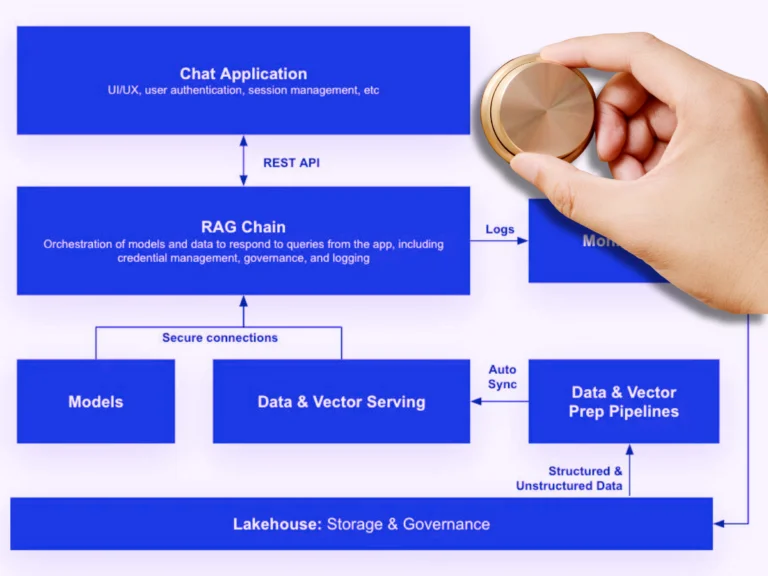
\includegraphics{Img/rag.jpg}

}

\caption{RAG vs Fine}

\end{figure}%

\subsubsection{\texorpdfstring{\textbf{¿Qué es RAG (Retrieval-Augmented
Generation)?}}{¿Qué es RAG (Retrieval-Augmented Generation)?}}\label{quuxe9-es-rag-retrieval-augmented-generation}

\textbf{Retrieval-Augmented Generation (RAG)} es una técnica avanzada de
IA que permite que un modelo de lenguaje grande (LLM) acceda a una base
de datos externa, actualizada y específica para responder preguntas en
tiempo real. En lugar de confiar únicamente en el conocimiento
preentrenado del modelo, RAG combina el poder de recuperación de datos
en tiempo real con las capacidades de un modelo de lenguaje, lo que
resulta en respuestas más precisas y contextualmente relevantes.

\textbf{Flujo de trabajo de RAG:} 1. \textbf{Procesamiento de la
consulta:} El usuario introduce una pregunta o solicitud en lenguaje
natural (por ejemplo, ``¿Cuál es el estado de mis envíos de proveedores
esta semana?''). 2. \textbf{Recuperación de datos:} El sistema busca en
bases de datos internas o externas los datos más relevantes para
responder la consulta. 3. \textbf{Integración con el LLM:} Los datos
recuperados se integran con la pregunta original y se introducen en el
modelo de lenguaje grande. 4. \textbf{Generación de la respuesta:} El
LLM procesa la información y genera una respuesta que combina el
contexto de la pregunta con los datos más recientes.

\textbf{Ventajas de RAG en la maquiladora:} - \textbf{Información en
tiempo real:} RAG permite que los directivos y gerentes tomen decisiones
basadas en los datos más actualizados, lo que es esencial en entornos de
producción rápida. - \textbf{Seguridad:} Los datos no se incorporan
directamente al modelo, sino que permanecen en la base de datos
controlada por la empresa, lo que mejora la seguridad y el control de
acceso. - \textbf{Costo eficiente:} Al evitar el reentrenamiento
completo de modelos grandes, RAG es más eficiente en costos a largo
plazo. - \textbf{Escalabilidad:} Se puede integrar fácilmente en
sistemas ya existentes, permitiendo su crecimiento sin complicaciones.

\textbf{Ejemplo en maquiladora:} Imagina que un supervisor de producción
quiere saber cuántas piezas de una componente crítica hay disponibles
para cumplir con una orden urgente. En lugar de buscar entre hojas de
cálculo o preguntar a varios departamentos, el supervisor solo necesita
hacer una consulta al sistema RAG: ``¿Cuántas piezas de X están
disponibles en inventario?''. El sistema buscará la respuesta en tiempo
real, accediendo a la base de datos interna, y proporcionará la
información exacta, mejorando así la eficiencia operativa.

\subsubsection{\texorpdfstring{\textbf{¿Qué es Fine
Tuning?}}{¿Qué es Fine Tuning?}}\label{quuxe9-es-fine-tuning}

\textbf{Fine Tuning} es el proceso de ajustar un modelo de IA ya
preentrenado para que sea óptimo en una tarea o dominio específico. Esto
se logra mediante el entrenamiento del modelo con un conjunto de datos
etiquetado y especializado que se ajusta a las necesidades particulares
de la maquila. Fine Tuning permite que un modelo generalista, como
GPT-4, se convierta en un experto en las particularidades del negocio.

\textbf{Proceso de Fine Tuning:} 1. \textbf{Entrenamiento en datos
especializados:} El modelo preentrenado recibe datos específicos de la
maquila, como patrones de producción, informes de calidad o reportes de
fallos de maquinaria. 2. \textbf{Ajuste de parámetros:} El modelo ajusta
sus parámetros internos para adaptarse mejor a los datos especializados.
3. \textbf{Optimización:} Después del ajuste, el modelo es capaz de
manejar tareas muy específicas de manera mucho más eficiente y precisa.
4. \textbf{Uso continuo:} El modelo entrenado puede ser mejorado
continuamente con nuevos datos, asegurando que se mantenga actualizado y
adaptado.

\textbf{Ventajas de Fine Tuning:} - \textbf{Especialización profunda:}
Fine Tuning permite que el modelo sea altamente especializado en las
operaciones de la maquila, lo que puede ser invaluable para tareas como
la predicción de fallos de maquinaria o la optimización de líneas de
producción. - \textbf{Adaptabilidad:} Es ideal para procesos que
requieren un conocimiento profundo y repetido de patrones históricos,
como la gestión de calidad o la evaluación de riesgos. - \textbf{Mejora
continua:} A medida que se recopilan más datos, el modelo puede seguir
ajustándose para mejorar su rendimiento.

\textbf{Ejemplo en maquiladora:} Un modelo de IA general puede predecir
cuándo fallará una máquina con base en datos generales de fallos. Sin
embargo, con Fine Tuning, el modelo puede ser ajustado para identificar
patrones específicos de fallos en las máquinas de la maquila, basándose
en datos históricos de esa misma planta. Esto permite predecir con mayor
precisión y prevenir paros inesperados en la producción.

\subsubsection{\texorpdfstring{\textbf{Comparación: RAG vs Fine
Tuning}}{Comparación: RAG vs Fine Tuning}}\label{comparaciuxf3n-rag-vs-fine-tuning}

\begin{longtable}[]{@{}
  >{\raggedright\arraybackslash}p{(\columnwidth - 4\tabcolsep) * \real{0.2519}}
  >{\raggedright\arraybackslash}p{(\columnwidth - 4\tabcolsep) * \real{0.3630}}
  >{\raggedright\arraybackslash}p{(\columnwidth - 4\tabcolsep) * \real{0.3852}}@{}}
\toprule\noalign{}
\begin{minipage}[b]{\linewidth}\raggedright
\textbf{Característica}
\end{minipage} & \begin{minipage}[b]{\linewidth}\raggedright
\textbf{RAG (Retrieval-Augmented Generation)}
\end{minipage} & \begin{minipage}[b]{\linewidth}\raggedright
\textbf{Fine Tuning}
\end{minipage} \\
\midrule\noalign{}
\endhead
\bottomrule\noalign{}
\endlastfoot
\textbf{Funcionalidad principal} & Recuperar datos en tiempo real y
combinarlos con la consulta del usuario. & Ajustar el modelo a tareas o
dominios muy específicos. \\
\textbf{Datos utilizados} & Base de datos externa, actualizada en tiempo
real. & Conjunto de datos especializado y etiquetado. \\
\textbf{Entrenamiento} & No requiere reentrenamiento. & Requiere
reentrenamiento especializado. \\
\textbf{Costo} & Menor costo, no requiere ajustes constantes del modelo.
& Costo más elevado por la necesidad de reentrenamiento. \\
\textbf{Escalabilidad} & Altamente escalable, fácil de integrar en
sistemas existentes. & Menos escalable, requiere actualizaciones
periódicas. \\
\textbf{Casos de uso} & Ideal para tareas en tiempo real como monitoreo
de inventarios, demanda y producción. & Excelente para tareas
especializadas como predicciones de mantenimiento o análisis de
calidad. \\
\end{longtable}

\subsubsection{\texorpdfstring{\textbf{Cuándo Usar RAG vs Cuándo Usar
Fine
Tuning}}{Cuándo Usar RAG vs Cuándo Usar Fine Tuning}}\label{cuuxe1ndo-usar-rag-vs-cuuxe1ndo-usar-fine-tuning}

\textbf{Usar RAG cuando:} - Necesitas acceso rápido a información
actualizada en tiempo real. - Tu negocio maneja grandes volúmenes de
datos dinámicos, como inventarios o transacciones diarias. - La
seguridad y privacidad de los datos son prioridades y prefieres mantener
los datos en una base externa.

\textbf{Usar Fine Tuning cuando:} - Tienes un problema específico que
requiere una solución altamente personalizada. - El modelo necesita
adaptarse a las particularidades de la maquila, como un proceso de
producción o análisis de datos de mantenimiento. - Los datos de tu
negocio son relativamente estables, y puedes justificar el costo de
entrenar el modelo.

\subsubsection{\texorpdfstring{\textbf{Ejemplo Completo: Optimización
del Mantenimiento Predictivo con Fine Tuning y
RAG}}{Ejemplo Completo: Optimización del Mantenimiento Predictivo con Fine Tuning y RAG}}\label{ejemplo-completo-optimizaciuxf3n-del-mantenimiento-predictivo-con-fine-tuning-y-rag}

Imagina que la maquiladora tiene un problema recurrente con una de sus
máquinas clave. Cada tres meses, la máquina se descompone, causando
retrasos y pérdidas. Quieres implementar una solución basada en IA para
predecir cuándo es probable que la máquina falle.

\textbf{Con Fine Tuning:} Primero, recopilas todos los datos históricos
sobre el uso de la máquina, el mantenimiento realizado y los momentos en
que ha fallado. Estos datos se utilizan para ajustar un modelo de IA
preentrenado, optimizándolo para detectar patrones específicos que
indican cuándo la máquina está en riesgo de fallar. El modelo se entrena
para predecir con precisión el momento en que será necesario el
mantenimiento preventivo.

\textbf{Con RAG:} Mientras tanto, implementas RAG para que el sistema
pueda acceder a datos en tiempo real sobre la máquina. El modelo RAG
puede responder a preguntas como ``¿Cuál es la condición actual de la
máquina X?'' o ``¿Cuándo se realizó el último mantenimiento?''. Con esta
información actualizada al instante, puedes tomar decisiones inmediatas
si algo parece estar fuera de lugar.

\subsection{}\label{section}

\textbf{Consideraciones Finales}

La implementación de RAG o Fine Tuning no es una elección de ``todo o
nada''. En muchas maquiladoras, la mejor opción es combinar ambos
enfoques para obtener lo mejor de los dos mundos. RAG permite que el
personal acceda a información crítica en tiempo real sin necesidad de
reentrenar modelos constantemente, mientras que Fine Tuning ofrece una
solución personalizada y altamente optimizada para tareas específicas.

Ambas tecnologías, cuando se utilizan de manera correcta, pueden
transformar radicalmente la maquiladora, automatizando tareas críticas,
mejorando la precisión en las decisiones y reduciendo los costos
operativos. La clave está en identificar qué procesos de tu maquiladora
se beneficiarán más de cada enfoque y planificar su implementación para
maximizar el retorno de la inversión.

Aquí te presento una tabla que compara los costos aproximados de
implementar un proyecto de IA utilizando \textbf{RAG
(Retrieval-Augmented Generation)} con una GPU \textbf{NVIDIA GeForce RTX
4090}, y \textbf{Fine Tuning}, basándonos en los costos de
entrenamiento, hardware y uso de token. He utilizado los datos
proporcionados de precios y escenarios comunes para ilustrar la
diferencia entre ambos enfoques:

\begin{longtable}[]{@{}
  >{\raggedright\arraybackslash}p{(\columnwidth - 4\tabcolsep) * \real{0.2147}}
  >{\raggedright\arraybackslash}p{(\columnwidth - 4\tabcolsep) * \real{0.3898}}
  >{\raggedright\arraybackslash}p{(\columnwidth - 4\tabcolsep) * \real{0.3955}}@{}}
\toprule\noalign{}
\begin{minipage}[b]{\linewidth}\raggedright
\textbf{Concepto}
\end{minipage} & \begin{minipage}[b]{\linewidth}\raggedright
\textbf{RAG (Retrieval-Augmented Generation)}
\end{minipage} & \begin{minipage}[b]{\linewidth}\raggedright
\textbf{Fine Tuning (Re-entrenamiento de IA)}
\end{minipage} \\
\midrule\noalign{}
\endhead
\bottomrule\noalign{}
\endlastfoot
\textbf{Costo de Hardware (NVIDIA RTX 4090)} & \$88,999 MXN (Tarjeta de
Video Gigabyte NVIDIA GeForce RTX 4090)
\href{https://www.cyberpuerta.mx/Computo-Hardware/Componentes/Tarjetas-de-Video/Tarjeta-de-Video-Gigabyte-NVIDIA-GeForce-RTX-4090-GAMING-OC-24GB-384-bit-GDDR6X-PCI-Express-4-0.html}{(link)}
& No se requiere GPU, solo servicio de reentrenamiento, dependiente de
nube. \\
\textbf{Costo de Infraestructura (Open Source)} & Uso de RAGFlow
open-source, costo 0 MXN en software, solo infraestructura (computo
local o nube). & Sin costo de hardware específico, depende de servicios
en la nube. \\
\textbf{Costo de Infraestructura (Privado)} & Licencias privadas de
software y servidores específicos para RAG pueden costar \$15,000 -
\$50,000 MXN según requerimientos de seguridad. & Costo variable, según
el uso en servicios como Google Cloud, AWS (Aproximadamente \$3,000 MXN
al mes). \\
\textbf{Costo de Entrenamiento (mensual)} & No es necesario
reentrenamiento, RAG utiliza bases de datos dinámicas. & \$3,000 MXN/mes
por reentrenamiento en un servicio de nube (dependiente del tamaño del
modelo y datos). \\
\textbf{Costo por Token (inferencia)} & No aplica para RAG. &
Aproximadamente \$0.001 USD por token (variará según el tamaño del
modelo). \\
\textbf{Escalabilidad} & Fácil de escalar mediante la integración de más
datos a la base de RAG. & Requiere ajustar continuamente el modelo con
nuevos datos para mejorar precisión. \\
\textbf{Seguridad y Privacidad} & Los datos permanecen en bases
controladas por la empresa. & Los datos entrenados podrían estar
expuestos al servicio de nube. \\
\textbf{Uso de Computo Local vs Nube} & Puede implementarse localmente
con hardware adecuado (GPU 4090). & Principalmente dependiente de la
nube para reentrenamiento y procesamiento. \\
\textbf{Tiempo de Implementación} & Rápida, ya que no requiere entrenar
modelos, solo ajustar la base de datos. & Toma más tiempo debido a la
necesidad de reentrenar el modelo regularmente. \\
\textbf{Costo Total Estimado Inicial (RAG)} & \textasciitilde{} \$48,999
MXN (tarjeta de video) + infraestructura en caso de ser privada. &
\textasciitilde{} \$3,000 MXN mensuales (sin hardware), pero con costos
crecientes por tokens y nube. \\
\end{longtable}

\subsection{Notas:}\label{notas}

\begin{itemize}
\tightlist
\item
  \textbf{RAG}: Utiliza hardware especializado como la \textbf{NVIDIA
  RTX 4090} para maximizar el procesamiento local si no se quiere
  depender de la nube. En sistemas abiertos (open-source), puede
  integrarse sin costo de licencias, pero con infraestructura privada
  puede aumentar los costos.
\item
  \textbf{Fine Tuning}: Se enfoca más en servicios en la nube con un
  costo mensual fijo por el reentrenamiento y un costo por token de uso
  dependiendo del servicio que se contrate.
\item
  **Perfil operacional depende, de la solución la Fine Tunning solo
  vasta con con desarrollador con conocimiento en el uso de Apis, pero
  en con la solución RAG se requiere un desarrollador MLDevOps mínimo
  por un par de meses.
\end{itemize}

\subsection{Capítulo: La Importancia de un Banco de Datos en la
Implementación de
IA}\label{capuxedtulo-la-importancia-de-un-banco-de-datos-en-la-implementaciuxf3n-de-ia}

En cualquier empresa que busque implementar inteligencia artificial (IA)
de manera seria y estratégica, uno de los aspectos más fundamentales es
la \textbf{gestión de datos}. Sin un \textbf{banco de datos sólido},
cualquier esfuerzo por adoptar la IA estará destinado al fracaso o, en
el mejor de los casos, a obtener resultados mediocres. La razón es
simple: la IA se alimenta de datos. Si no cuentas con datos limpios,
organizados y, sobre todo, relevantes, las predicciones y optimizaciones
que puedan hacer los modelos serán ineficaces y hasta peligrosas para la
toma de decisiones.

\subsubsection{El Papel Crucial del Banco de
Datos}\label{el-papel-crucial-del-banco-de-datos}

Cuando hablamos de IA, no estamos solo refiriéndonos a software
inteligente que toma decisiones en lugar de los humanos. Hablamos de
\textbf{análisis de patrones complejos}, \textbf{predicciones basadas en
datos históricos}, y \textbf{automatización de procesos}. Para que esto
ocurra, el sistema necesita algo muy importante: \textbf{datos de
calidad}. Y estos datos no son una simple recolección al azar de
información, sino una estructura organizada que te permita manejar de
forma efectiva el \textbf{historial de operaciones}, las
\textbf{variables críticas}, y los \textbf{documentos necesarios} para
que la IA aprenda, evolucione y, lo más importante, \textbf{genere valor
para la maquila}.

Sin un banco de datos bien estructurado, estarías improvisando cada vez
que el sistema necesita información para hacer predicciones o tomar
decisiones. Este banco no es solo un espacio donde se guarda
información, es un \textbf{repositorio estratégico} que, bien
gestionado, puede ser la clave del éxito de cualquier implementación de
IA. A continuación, desglosaremos cómo debería estructurarse este banco
de datos en dos grandes partes.

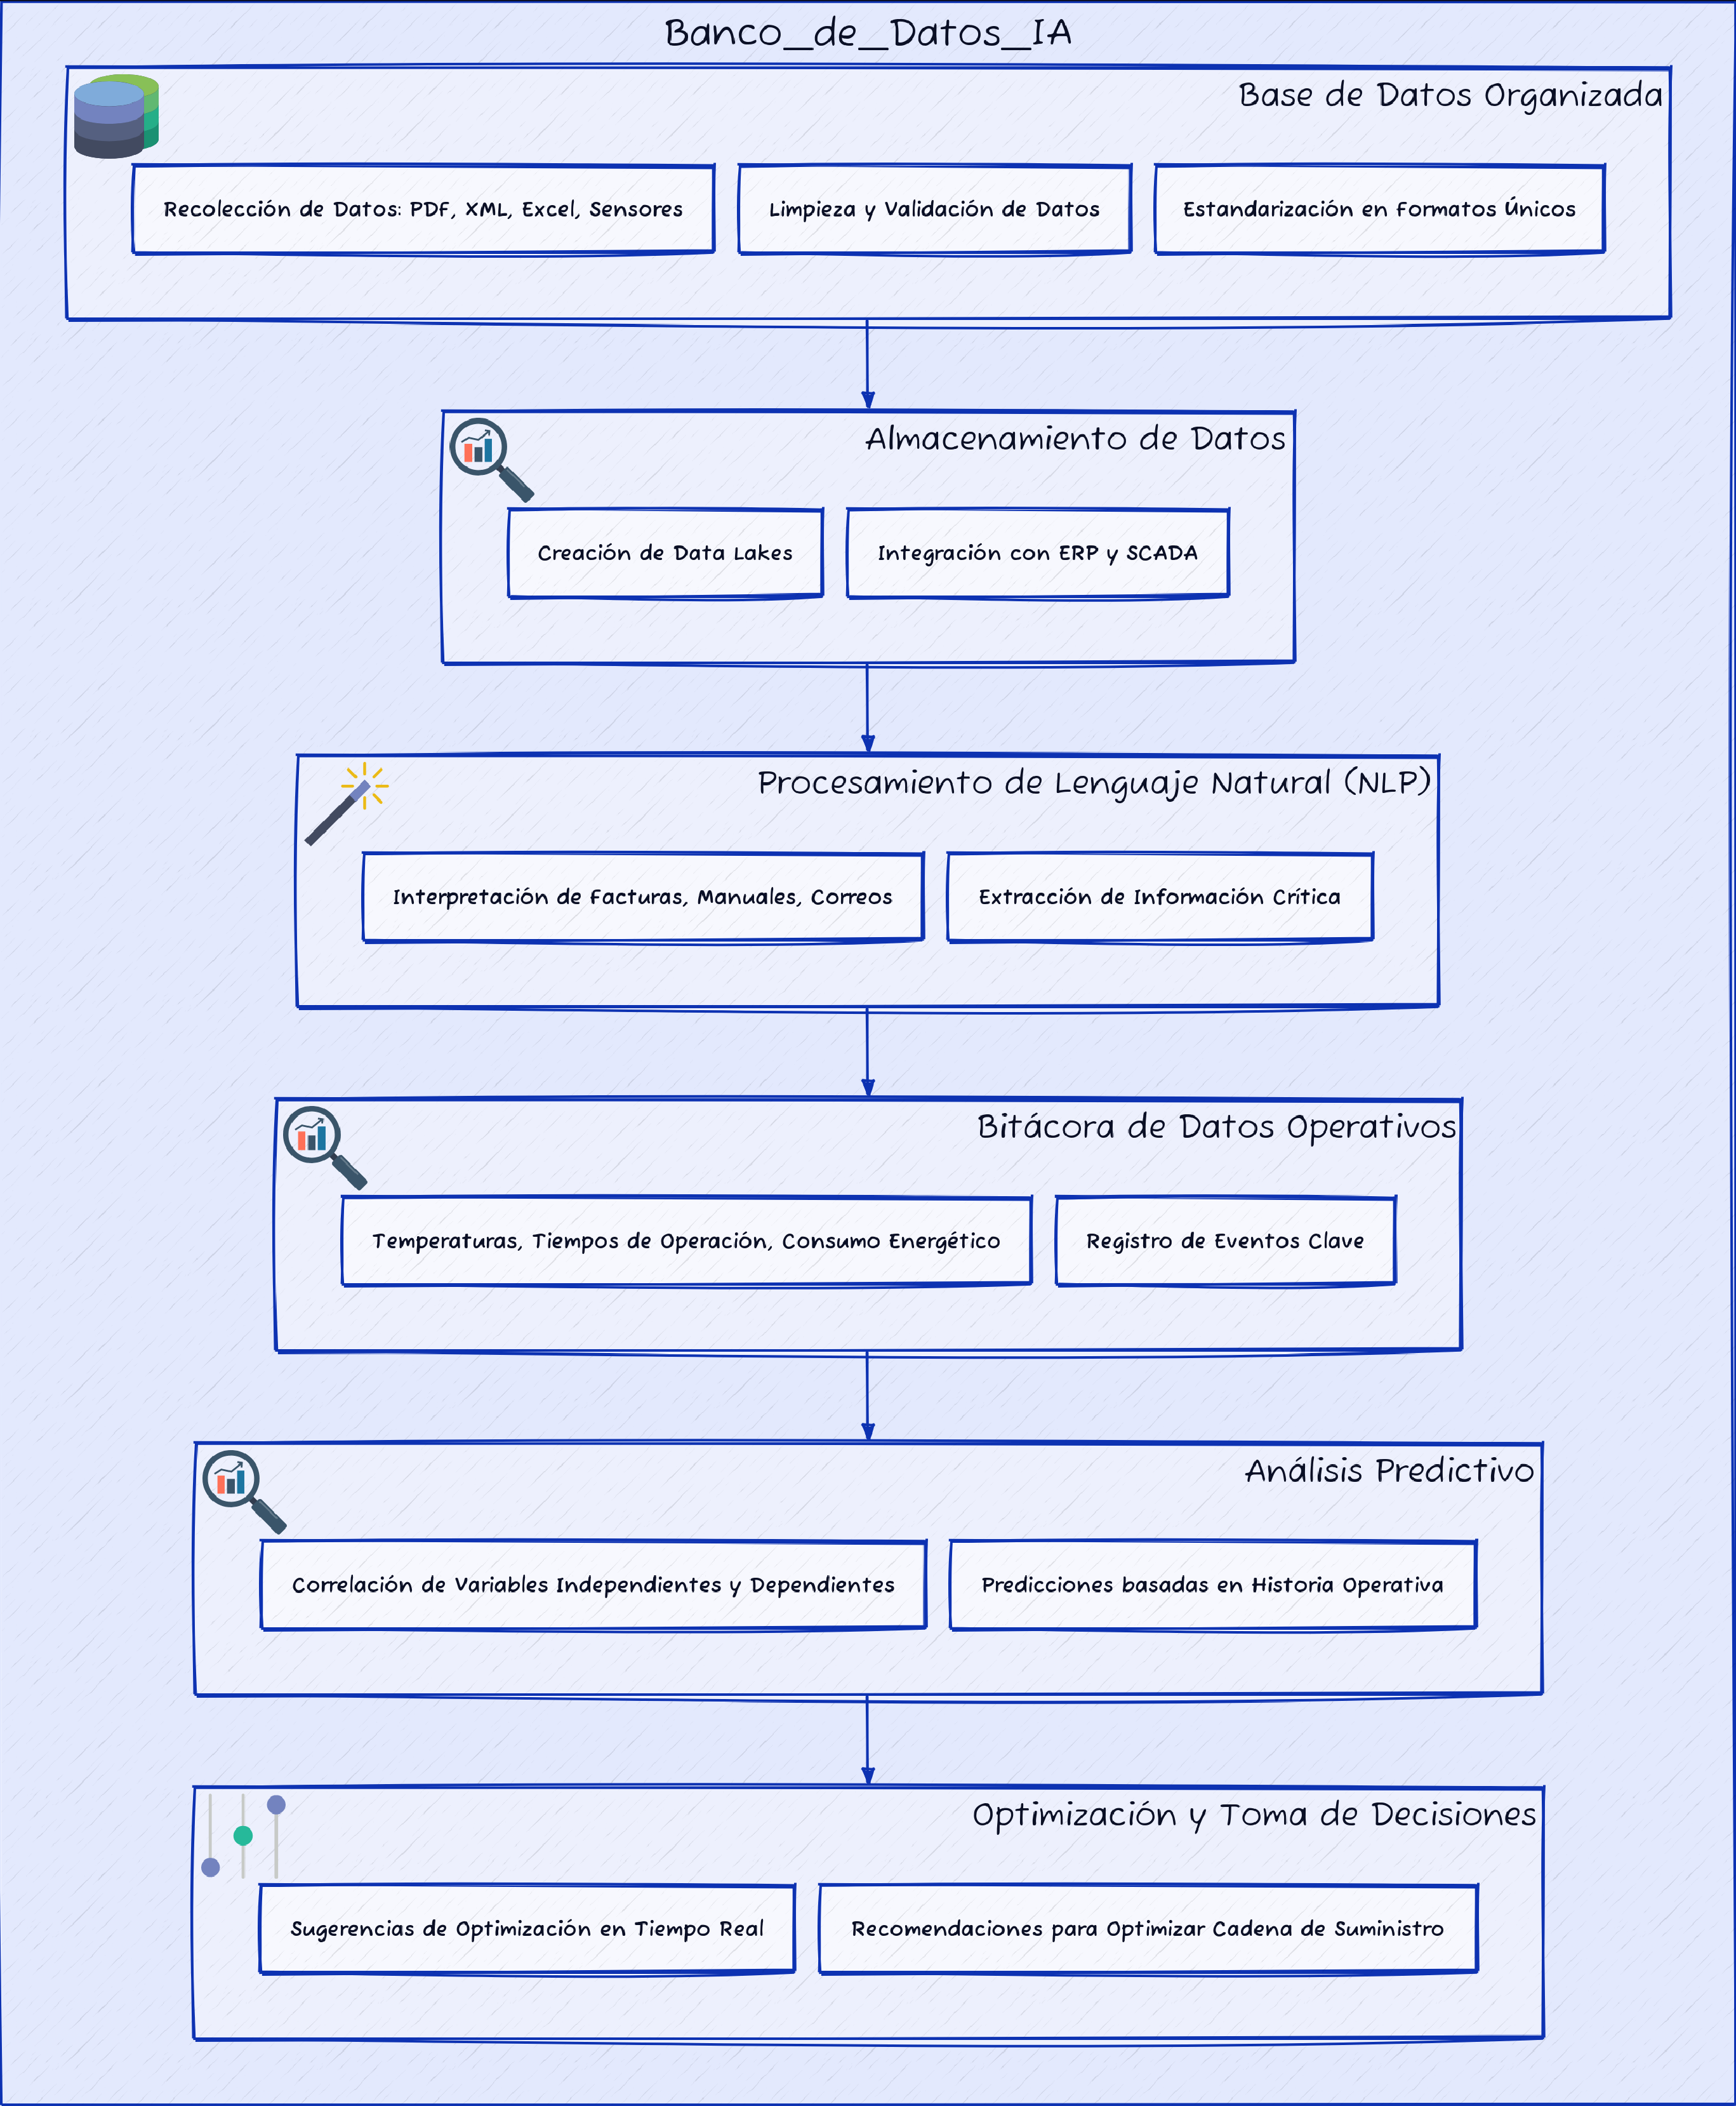
\includegraphics[width=1\textwidth,height=\textheight]{index_files/mediabag/diagram-7.pdf}

\begin{enumerate}
\def\labelenumi{\arabic{enumi}.}
\tightlist
\item
  \textbf{Lenguaje Natural y Lógica de Negocio}
\end{enumerate}

La primera parte del banco de datos que debes estructurar estará
enfocada en toda la información relacionada con \textbf{lenguaje
natural}. Aquí es donde embonamos y organizamos toda la \textbf{lógica
de negocio} de la maquila, desde documentos que guían la operación hasta
los intercambios diarios que ocurren entre los distintos departamentos y
actores involucrados.

Dentro de esta sección de lenguaje natural se incluyen varios tipos de
información:

\begin{itemize}
\item
  \textbf{Facturas Electrónicas y Documentación Comercial}: Desde
  \textbf{facturas en PDF, XML}, hasta formatos electrónicos más
  avanzados. Estos documentos no solo registran las transacciones
  económicas de la maquila, sino que también contienen datos clave sobre
  los productos, proveedores, tiempos de entrega, costos y más. Al tener
  estas facturas integradas en el banco de datos, la IA puede realizar
  análisis avanzados como predecir qué proveedores tienden a entregar
  tarde o cómo se puede optimizar la cadena de suministro en función de
  los costos históricos.
\item
  \textbf{Manuales y Guías Operativas}: Estos documentos son vitales
  para el funcionamiento de cualquier operación industrial. Imagina un
  manual de operación para maquinaria, o un procedimiento detallado
  sobre cómo manejar un sistema de control de calidad. La IA puede
  analizar esta información para recomendar cambios o generar
  procedimientos más eficientes basados en datos históricos de fallas o
  errores humanos.
\item
  \textbf{Correos Electrónicos y Comunicaciones Internas}: La
  comunicación interna es una mina de oro para la IA. Correos que
  confirman pedidos, comunicaciones entre los distintos departamentos y
  hasta las conversaciones sobre cambios en la planificación de la
  producción. Toda esta información puede ser procesada para crear
  patrones de comportamiento y hacer recomendaciones más precisas.
\item
  \textbf{Exámenes de Calidad y Auditorías}: Los reportes de calidad
  realizados por inspectores o auditores son una fuente clave de
  información. Al almacenar estos datos, puedes implementar IA para
  detectar patrones de defectos, correlacionar las fallas con cambios en
  el proceso de producción o predecir futuras no conformidades antes de
  que ocurran.
\end{itemize}

\subsubsection{¿Por qué el Lenguaje Natural es
Importante?}\label{por-quuxe9-el-lenguaje-natural-es-importante}

Toda esta información escrita o digitalizada es entendible para los
humanos, pero ¿cómo ayuda a la IA? Aquí es donde entra el
\textbf{Procesamiento de Lenguaje Natural (NLP)}. El NLP permite que la
IA entienda documentos escritos, correos, y cualquier tipo de lenguaje
humano, interpretando la lógica detrás de esos textos para hacer
sugerencias y tomar decisiones. Un banco de datos bien estructurado con
toda esta información en formato digital permite que la IA analice
toneladas de datos que de otra forma solo estarían accesibles a humanos,
y lo haga de manera rápida, precisa y a gran escala.

\begin{enumerate}
\def\labelenumi{\arabic{enumi}.}
\setcounter{enumi}{1}
\tightlist
\item
  \textbf{Bitácora de Datos Operativos y Variables}
\end{enumerate}

La segunda parte de este banco de datos está dedicada a la
\textbf{bitácora de datos operativos}, es decir, la información que
proviene directamente de las operaciones de la maquila. A diferencia del
lenguaje natural, aquí hablamos de \textbf{datos estructurados}, muchas
veces numéricos, que describen cómo funcionan las máquinas, cómo fluyen
los materiales y cómo se cumplen los ciclos de producción.

En esta bitácora se incluye información como:

\begin{itemize}
\item
  \textbf{Variables Operativas Críticas}: Estas pueden ser las
  temperaturas de las máquinas, los tiempos de operación, las
  velocidades de producción, las tasas de consumo de energía, o incluso
  el uso de recursos como el agua o el gas. Cada dato cuenta, porque
  cada uno puede afectar el resultado final de la producción. Una IA
  puede utilizar esta información para sugerir ajustes que optimicen la
  operación, reducir costos y prevenir fallos.
\item
  \textbf{Fechas y Tiempos de Operación}: Registrar cuándo suceden
  ciertos eventos es clave para entender el contexto en el que se
  producen los resultados. Ejemplo: si una máquina falla regularmente a
  ciertas horas del día, la IA puede detectar patrones y recomendar
  cambios en los turnos de operación o en los tiempos de mantenimiento.
\item
  \textbf{Métricas de Producción}: Desde el número de unidades
  producidas hasta el scrap generado, todas estas métricas proporcionan
  una \textbf{historia operacional} que es vital para cualquier análisis
  predictivo. La IA puede analizar estas métricas y determinar qué
  procesos son los más eficientes y cuáles necesitan mejoras.
\item
  \textbf{Variables Dependientes e Independientes}: Estas son las
  variables que están afectando el desempeño general de la maquila. Las
  \textbf{variables independientes} son aquellas que controlas
  directamente, como las horas de operación, la cantidad de material
  utilizado, o los parámetros de una máquina. Las \textbf{variables
  dependientes} son los resultados, como la cantidad de productos
  defectuosos o el tiempo de inactividad. La IA puede correlacionar
  ambos tipos de variables para sugerir mejoras en tiempo real.
\end{itemize}

\subsection{Importancia de la Historia Operativa y Predicciones de
IA}\label{importancia-de-la-historia-operativa-y-predicciones-de-ia}

Para tener un modelo de IA que realmente pueda hacer predicciones
precisas, es necesario contar con una \textbf{historia operativa} bien
documentada. Si quieres implementar un sistema de \textbf{mantenimiento
predictivo}, necesitas al menos \textbf{tres a cuatro meses} de datos de
operación para que la IA pueda aprender patrones y hacer predicciones.
Sin estos datos, cualquier predicción sería meramente especulativa.

Lo mismo aplica si quieres optimizar los niveles de inventario o la
planificación de producción. Sin la información de cuándo se hicieron
las entregas, cómo fluctuó la demanda o cómo variaron los tiempos de
ciclo de producción, el modelo de IA no puede hacer recomendaciones
confiables.

\subsection{Recomendaciones para Mantener un Banco de
Datos}\label{recomendaciones-para-mantener-un-banco-de-datos}

\begin{enumerate}
\def\labelenumi{\arabic{enumi}.}
\item
  \textbf{Calidad de los Datos}: La calidad es crítica. Si metes datos
  erróneos, obtendrás resultados erróneos. Asegúrate de que los datos
  ingresados estén bien validados y que no contengan errores
  significativos.
\item
  \textbf{Estandarización de Formatos}: Todos los datos deben estar en
  formatos estandarizados para evitar problemas de compatibilidad y
  facilitar el análisis. Ya sea que uses XML, JSON, o algún formato de
  base de datos, asegúrate de que todos los equipos trabajen con los
  mismos estándares.
\item
  \textbf{Frecuencia de Actualización}: Entre más reciente sea la
  información, más precisos serán los análisis. Debes diseñar procesos
  para que los datos sean actualizados de manera constante y automática.
  La automatización en este sentido es clave.
\item
  \textbf{Accesibilidad}: El banco de datos debe ser fácilmente
  accesible para todos los equipos relevantes, desde los gerentes hasta
  los operadores, para que puedan interactuar con la IA y sacar el
  máximo provecho de sus capacidades.
\end{enumerate}

\subsection{Un Proyecto de IA Sin un Banco de Datos es como una Fábrica
Sin
Electricidad}\label{un-proyecto-de-ia-sin-un-banco-de-datos-es-como-una-fuxe1brica-sin-electricidad}

En resumen, un banco de datos es la \textbf{columna vertebral} de
cualquier proyecto de IA exitoso. Sin datos, la IA no tiene de dónde
aprender, y sin aprendizaje, no puede optimizar procesos ni mejorar la
operación. La maquila que logre organizar sus datos de manera eficiente
y aprovechable tendrá una ventaja competitiva enorme, ya que podrá
implementar IA en todas sus áreas, desde producción hasta logística,
mejorando así la productividad, reduciendo costos y aumentando la
calidad de sus productos.

Este banco de datos no solo te permitirá manejar la operación actual,
sino que te preparará para los desafíos del futuro, donde la IA no será
una opción, sino una \textbf{necesidad} para competir en un mundo cada
vez más automatizado y centrado en los datos.

¡Es hora de empezar a construir ese banco de datos!

\bookmarksetup{startatroot}

\chapter{Futuro}\label{futuro}

\bookmarksetup{startatroot}

\chapter{Recomendaciones}\label{recomendaciones}

\bookmarksetup{startatroot}

\chapter{\texorpdfstring{\textbf{Glosario de Términos Técnicos y
Expresiones
Locales}}{Glosario de Términos Técnicos y Expresiones Locales}}\label{glosario-de-tuxe9rminos-tuxe9cnicos-y-expresiones-locales}

Este glosario está diseñado para ayudar a los lectores a comprender los
términos técnicos y las expresiones coloquiales utilizadas a lo largo
del libro. Incluye tanto conceptos fundamentales de la inteligencia
artificial como vocabulario local de Ciudad Juárez, con el objetivo de
hacer el contenido más accesible y comprensible para todos.

\begin{center}\rule{0.5\linewidth}{0.5pt}\end{center}

\section{\texorpdfstring{\textbf{Términos
Técnicos}}{Términos Técnicos}}\label{tuxe9rminos-tuxe9cnicos}

\begin{enumerate}
\def\labelenumi{\arabic{enumi}.}
\tightlist
\item
  \textbf{Inteligencia Artificial (IA)}:

  \begin{itemize}
  \tightlist
  \item
    \textbf{Definición}: Tecnología que permite a las máquinas realizar
    tareas que normalmente requieren inteligencia humana, como el
    reconocimiento de patrones, la toma de decisiones, el aprendizaje y
    la resolución de problemas.
  \item
    \textbf{Posible Confusión}: Algunos lectores pueden asociar la IA
    solo con robots o procesos futuristas. En este libro, IA se refiere
    a herramientas prácticas que ya se están utilizando en la industria
    maquiladora para optimizar la producción y mejorar la eficiencia.
  \item
    \textbf{Ejemplo}: ``La IA está transformando la forma en que las
    maquiladoras operan al automatizar procesos clave.''
  \end{itemize}
\item
  \textbf{IA Simbólica}:

  \begin{itemize}
  \tightlist
  \item
    \textbf{Definición}: Un enfoque de la inteligencia artificial que se
    basa en representar el conocimiento y tomar decisiones a través de
    reglas lógicas predefinidas (del tipo ``si-entonces'').
  \item
    \textbf{Posible Confusión}: A diferencia del ``Machine Learning'',
    la IA simbólica no aprende de los datos; sigue estrictamente las
    reglas que se le han programado.
  \item
    \textbf{Ejemplo}: ``En la maquila, la IA simbólica puede ser usada
    para controlar la temperatura de las máquinas siguiendo reglas
    claras.''
  \end{itemize}
\item
  \textbf{Machine Learning (Aprendizaje Automático)}:

  \begin{itemize}
  \tightlist
  \item
    \textbf{Definición}: Rama de la inteligencia artificial que permite
    a las máquinas aprender a partir de datos y mejorar su rendimiento
    sin ser programadas explícitamente para cada tarea.
  \item
    \textbf{Posible Confusión}: Los lectores podrían no distinguir
    claramente entre IA simbólica y Machine Learning. Es importante
    destacar que mientras la IA simbólica sigue reglas fijas, el Machine
    Learning ``aprende'' de los datos y ajusta sus comportamientos en
    consecuencia.
  \item
    \textbf{Ejemplo}: ``El Machine Learning se usa en la maquila para
    predecir cuándo una máquina va a fallar basándose en datos
    históricos.''
  \end{itemize}
\item
  \textbf{Razonamiento Automatizado}:

  \begin{itemize}
  \tightlist
  \item
    \textbf{Definición}: La capacidad de una IA para tomar decisiones o
    resolver problemas complejos siguiendo las reglas y el conocimiento
    almacenado en su base de datos.
  \item
    \textbf{Posible Confusión}: Algunos pueden pensar que la IA
    ``razona'' de manera humana. En realidad, su razonamiento es lógico
    y basado en datos, no emocional o intuitivo.
  \item
    \textbf{Ejemplo}: ``El razonamiento automatizado permite que la IA
    en la maquila determine cuándo una máquina necesita mantenimiento.''
  \end{itemize}
\item
  \textbf{Procesamiento del Lenguaje Natural (NLP)}:

  \begin{itemize}
  \tightlist
  \item
    \textbf{Definición}: Tecnología que permite a las máquinas
    comprender, interpretar y generar lenguaje humano, facilitando la
    interacción entre humanos y computadoras mediante el habla o el
    texto.
  \item
    \textbf{Posible Confusión}: Puede haber confusión sobre la capacidad
    de las máquinas para ``entender'' realmente el lenguaje humano. Es
    importante aclarar que las máquinas procesan patrones y palabras,
    pero no comprenden como un humano lo haría.
  \item
    \textbf{Ejemplo}: ``El procesamiento del lenguaje natural permite
    que una máquina interprete las órdenes de voz que le da un operador
    en la planta.''
  \end{itemize}
\item
  \textbf{Visión por Computadora}:

  \begin{itemize}
  \tightlist
  \item
    \textbf{Definición}: Tecnología que permite a las máquinas analizar
    y ``ver'' imágenes o videos, identificando patrones, objetos o
    personas.
  \item
    \textbf{Posible Confusión}: Algunos podrían confundir esta
    tecnología con simples cámaras de vigilancia. Sin embargo, la visión
    por computadora implica análisis avanzado de las imágenes para tomar
    decisiones.
  \item
    \textbf{Ejemplo}: ``La visión por computadora puede detectar
    defectos en productos ensamblados en la maquila en tiempo real.''
  \end{itemize}
\item
  \textbf{Sistemas Multiagente}:

  \begin{itemize}
  \tightlist
  \item
    \textbf{Definición}: Conjunto de inteligencias artificiales que
    trabajan en conjunto, colaborando o compitiendo entre sí para
    resolver problemas complejos.
  \item
    \textbf{Posible Confusión}: Puede resultar confuso si el lector no
    está familiarizado con el concepto de ``agentes''. Aquí se refiere a
    unidades individuales de IA que interactúan para completar tareas
    más grandes.
  \item
    \textbf{Ejemplo}: ``En una maquila, los sistemas multiagente pueden
    gestionar el flujo de trabajo entre robots y humanos para optimizar
    la producción.''
  \end{itemize}
\item
  \textbf{Automatización}:

  \begin{itemize}
  \tightlist
  \item
    \textbf{Definición}: Uso de tecnología, como la IA, para realizar
    tareas con poca o ninguna intervención humana.
  \item
    \textbf{Posible Confusión}: Algunas personas pueden asociar la
    automatización solo con la robótica física. Aquí también incluye
    procesos digitales y la toma de decisiones en la planta.
  \item
    \textbf{Ejemplo}: ``La automatización ha permitido que las líneas de
    producción en Juárez operen sin interrupciones.''
  \end{itemize}
\item
  \textbf{Optimización}:

  \begin{itemize}
  \tightlist
  \item
    \textbf{Definición}: Proceso en el que la IA busca la mejor solución
    entre un conjunto de opciones, ajustando variables para obtener el
    máximo rendimiento o eficiencia.
  \item
    \textbf{Posible Confusión}: Puede confundirse con simplemente
    ``mejorar''. Optimización implica encontrar la mejor solución
    posible dentro de un contexto específico.
  \item
    \textbf{Ejemplo}: ``La IA optimiza el uso de energía en la planta
    ajustando los tiempos de operación de las máquinas.''
  \end{itemize}
\item
  \textbf{Mantenimiento Predictivo}:

  \begin{itemize}
  \tightlist
  \item
    \textbf{Definición}: Uso de datos y tecnologías como el Machine
    Learning para predecir fallos en maquinaria o equipos antes de que
    ocurran.
  \item
    \textbf{Posible Confusión}: Puede confundirse con mantenimiento
    preventivo. La diferencia es que el mantenimiento predictivo se basa
    en datos y predicciones, no solo en un calendario fijo.
  \item
    \textbf{Ejemplo}: ``El mantenimiento predictivo evita que las
    máquinas se detengan inesperadamente, ahorrando tiempo y dinero.''
  \end{itemize}
\end{enumerate}

\begin{center}\rule{0.5\linewidth}{0.5pt}\end{center}

\subsection{\texorpdfstring{\textbf{Expresiones Locales y
Coloquiales}}{Expresiones Locales y Coloquiales}}\label{expresiones-locales-y-coloquiales}

\begin{enumerate}
\def\labelenumi{\arabic{enumi}.}
\tightlist
\item
  \textbf{Rifar}:

  \begin{itemize}
  \tightlist
  \item
    \textbf{Definición}: Esforzarse mucho o hacer las cosas bien. En el
    contexto de este libro, se refiere a trabajar duro en la
    maquiladora.
  \item
    \textbf{Posible Confusión}: Para lectores de fuera de México, esta
    expresión puede no tener un significado claro.
  \item
    \textbf{Ejemplo}: ``Los empleados de la maquila se rifan todos los
    días para cumplir con los objetivos de producción.''
  \end{itemize}
\item
  \textbf{Compa}:

  \begin{itemize}
  \tightlist
  \item
    \textbf{Definición}: Término coloquial para referirse a un amigo o
    compañero. Es común en Ciudad Juárez y otras partes de México.
  \item
    \textbf{Posible Confusión}: Algunos lectores podrían no estar
    familiarizados con el término y podrían malinterpretar su uso.
  \item
    \textbf{Ejemplo}: ``Este libro está escrito como si estuvieras
    platicando con un compa que sabe del tema.''
  \end{itemize}
\item
  \textbf{Chido}:

  \begin{itemize}
  \tightlist
  \item
    \textbf{Definición}: Expresión coloquial mexicana que significa
    ``bueno'' o ``genial''.
  \item
    \textbf{Posible Confusión}: Si el lector no es mexicano, puede no
    entender el significado de ``chido''.
  \item
    \textbf{Ejemplo}: ``La ubicación de Ciudad Juárez es chida para las
    empresas maquiladoras debido a su cercanía con Estados Unidos.''
  \end{itemize}
\item
  \textbf{Broncas}:

  \begin{itemize}
  \tightlist
  \item
    \textbf{Definición}: Problemas o dificultades.
  \item
    \textbf{Posible Confusión}: Algunos lectores podrían no estar
    familiarizados con esta expresión.
  \item
    \textbf{Ejemplo}: ``A pesar de las broncas con el crecimiento
    descontrolado, la maquila sigue siendo el motor económico de la
    ciudad.''
  \end{itemize}
\item
  \textbf{Jale}:

  \begin{itemize}
  \tightlist
  \item
    \textbf{Definición}: Término coloquial para referirse al trabajo o
    empleo.
  \item
    \textbf{Posible Confusión}: Lectores de fuera de México pueden no
    saber que significa ``Jale''.
  \item
    \textbf{Ejemplo}: ``La maquiladora sigue generando mucha Jale en la
    región, especialmente para las mujeres.''
  \end{itemize}
\item
  \textbf{Relajo}:

  \begin{itemize}
  \tightlist
  \item
    \textbf{Definición}: En este contexto, puede significar tanto
    diversión como caos o desorden.
  \item
    \textbf{Posible Confusión}: ``Relajo'' puede interpretarse como algo
    positivo (diversión) o negativo (caos), según el contexto.
  \item
    \textbf{Ejemplo}: ``Los soldados venían a Juárez a tirar relajo, lo
    que impulsó la economía local por un tiempo.''
  \end{itemize}
\item
  \textbf{Mancha de aceite}:

  \begin{itemize}
  \tightlist
  \item
    \textbf{Definición}: Expresión utilizada para describir un
    crecimiento desordenado y rápido, generalmente en el contexto
    urbano.
  \item
    \textbf{Posible Confusión}: Podría ser una metáfora difícil de
    entender para lectores internacionales.
  \item
    \textbf{Ejemplo}: ``La ciudad creció como mancha de aceite, con
    colonias surgiendo sin planificación adecuada.''
  \end{itemize}
\item
  \textbf{Sacar de onda}:

  \begin{itemize}
  \tightlist
  \item
    \textbf{Definición}: Expresión que significa ``confundir'' o
    ``desconcertar'' a alguien.
  \item
    \textbf{Posible Confusión}: Lectores de fuera de México podrían no
    entender esta expresión
  \end{itemize}
\end{enumerate}

. - \textbf{Ejemplo}: ``No te saques de onda si ves términos juarenses
en el libro, es parte de nuestra identidad.''

\begin{enumerate}
\def\labelenumi{\arabic{enumi}.}
\setcounter{enumi}{8}
\tightlist
\item
  \textbf{Andar al tiro}:

  \begin{itemize}
  \tightlist
  \item
    \textbf{Definición}: Estar atento o preparado.
  \item
    \textbf{Posible Confusión}: La expresión no es universalmente
    conocida, pero es común en México.
  \item
    \textbf{Ejemplo}: ``Es necesario andar al tiro porque las
    tecnologías de IA avanzan rápidamente.''
  \end{itemize}
\item
  \textbf{Morra(s)}:

  \begin{itemize}
  \tightlist
  \item
    \textbf{Definición}: Término coloquial para referirse a una mujer o
    mujeres jóvenes.
  \item
    \textbf{Posible Confusión}: Puede que no sea un término conocido por
    todos los lectores.
  \item
    \textbf{Ejemplo}: ``En los setentas, muchas morras encontraron
    trabajo en las maquilas de Juárez.''
  \end{itemize}
\end{enumerate}

\bookmarksetup{startatroot}

\chapter*{References}\label{references}
\addcontentsline{toc}{chapter}{References}

\markboth{References}{References}

\phantomsection\label{refs}
\begin{CSLReferences}{0}{1}
\subsection*{Referencias}\label{referencias-1}
\addcontentsline{toc}{subsection}{Referencias}

\begin{enumerate}
\def\labelenumi{\arabic{enumi}.}
\tightlist
\item
  Oscar Martínez, \emph{Ciudad Juárez: El auge de una ciudad fronteriza
  a partir de 1848}, FCE, México, 1982.
\item
  ``La Frontera norte, diagnóstico y perspectivas'', Dirección General
  de Estadística, S.I.C. s/f, mimeo.
\item
  Thomas Madison, \emph{Reseña anual de la industria maquiladora},
  SUGUMEX, México, 1990.
\item
  Bass Zavala, Sonia. ``El crecimiento urbano en Ciudad Juárez,
  1950-2000. Un acercamiento socio-histórico a la evolución desordenada
  de una ciudad de la frontera norte.'' \emph{Chihuahua Hoy} (2013):
  247-289.
\item
  ``La Frontera norte, diagnóstico y perspectivas'', Dirección General
  de Estadística, S.I.C. s/f, mimeo.
\item
  Diario de Juárez, 21 a 24 de agosto de 1981.
\item
  El Fronterizo, 25 de agosto de 1974.
\item
  Guadalupe Ramos, Norte, 9 de febrero de 1994, p.~4A.
\item
  Diario de Juárez, 22 de mayo de 1991.
\item
  Diario de Juárez, 7 de febrero de 1991.
\item
  Declaración de José Manuel Luna, promotor de AMACH, \emph{Novedades},
  20 de enero de 1985.
\item
  Vega, Luis. ``La transformación de la industria maquiladora en la era
  digital.'' \emph{El Financiero}, 2023.
\item
  Secretaría de Economía. ``Informe Anual sobre la Industria
  Maquiladora''. Gobierno de México, 2022.
\end{enumerate}

\end{CSLReferences}

\textbackslash end\{document\}


\backmatter

\backmatter
\printbibliography

\end{document}
